\documentclass[11pt]{article}
\usepackage[T1]{fontenc}
\usepackage{amsmath,amssymb,amsthm}
\usepackage[margin=1in]{geometry}
\usepackage[hidelinks]{hyperref}
\usepackage{tikz}
\usepackage[ruled,vlined,linesnumbered]{algorithm2e}
\DontPrintSemicolon
\SetAlFnt{\small}
\SetAlCapFnt{\small}
\SetKw{Continue}{continue}
\SetKw{Reject}{reject}
\AddToHook{env/algorithm/before}{\par\medskip}
\AddToHook{env/algorithm/after}{\par\medskip}
\DeclareRobustCommand{\HullData}{\textnormal{\textsc{HullData}}}
\DeclareRobustCommand{\EndpointCode}{\textnormal{\textsc{EndpointCode}}}
\DeclareRobustCommand{\IntervalCover}{\textnormal{\textsc{IntervalCover}}}
\DeclareRobustCommand{\BatchOrders}{\textnormal{\textsc{BatchOrders}}}
\DeclareRobustCommand{\ExpectedTree}{\textnormal{\textsc{ExpectedTree}}}
\DeclareRobustCommand{\PriorityTrial}{\textnormal{\textsc{PriorityTrial}}}
\DeclareRobustCommand{\GradeDP}{\textnormal{\textsc{GradeDP}}}
\DeclareRobustCommand{\SlotDP}{\textnormal{\textsc{SlotDP}}}
\DeclareRobustCommand{\HybridTree}{\textnormal{\textsc{HybridTree}}}
\DeclareRobustCommand{\ExactTree}{\textnormal{\textsc{ExactTree}}}
\DeclareRobustCommand{\Rollout}{\textnormal{\textsc{Rollout}}}

\newtheorem{theorem}{Theorem}[section]
\newtheorem{lemma}[theorem]{Lemma}
\newtheorem{proposition}[theorem]{Proposition}
\newtheorem{claim}{Claim}[section]
\newtheorem{corollary}[theorem]{Corollary}
\theoremstyle{definition}
\newtheorem{definition}[theorem]{Definition}
\theoremstyle{remark}
\newtheorem{remark}[theorem]{Remark}
\newcommand{\HH}{\mathcal H}
\newcommand{\LL}{\mathcal L}
\newcommand{\MSSC}{\operatorname{MSSC}}
\newcommand{\OPT}{\operatorname{OPT}}
% Compact source annotations for nontrivial steps in displayed calculations.
\newcommand{\byref}[3]{\overset{\text{\scriptsize #1~\ref{#2}}}{#3}}
\newsavebox{\proofstrategybox}
\newenvironment{proofstrategy}
 {\par\medskip\noindent\begin{lrbox}{\proofstrategybox}%
  \begin{minipage}{\dimexpr\linewidth-2\fboxsep-2\fboxrule\relax}%
  \small\textbf{Proof strategy.}\par\smallskip}
 {\end{minipage}\end{lrbox}%
  \fcolorbox{blue!35!black}{blue!3}{\usebox{\proofstrategybox}}\par\medskip}
\newsavebox{\parameterchoicebox}
\newenvironment{parameterchoice}
 {\par\medskip\noindent\begin{lrbox}{\parameterchoicebox}%
  \begin{minipage}{\dimexpr\linewidth-2\fboxsep-2\fboxrule\relax}%
  \small\textbf{Parameter calibration.}\par\smallskip}
 {\end{minipage}\end{lrbox}%
  \fcolorbox{gray!45}{gray!5}{\usebox{\parameterchoicebox}}\par\medskip}
\newenvironment{symboltable}
 {\begin{center}\small
  \begin{tabular}{@{}p{0.20\linewidth}p{0.72\linewidth}@{}}
  \textbf{Symbol}&\textbf{Meaning}\\\hline}
 {\end{tabular}\end{center}}

\title{Line-Query Decision Trees:\\
Approximation and Strong NP-Completeness}
\author{}
\date{October 14, 2026}
\hypersetup{
  pdftitle={Line-Query Decision Trees: Approximation and Strong NP-Completeness},
  pdfsubject={Supplied-query approximation algorithms, randomized mixing, and strong NP-completeness}
}

\begin{document}
\maketitle

\begin{abstract}
The Line-Query Decision Tree problem is to identify a hidden planar
point using only a supplied separating family of line queries. We give
deterministic polynomial approximation factors below $4.464966$ for
maximum depth and $5.182976$ for arbitrary-prior expected depth, along
with quasipolynomial
$(2+\varepsilon)$ approximations for both objectives. A shared
geometric structure underlies both algorithms: for flat states,
Helly's theorem gives a common majority witness, and
the convex hull turns each hypothesis's positive answers into a
circular interval. The algorithms first discover the interval pattern
containing the target, then decode its endpoints. Restricting an
optimal tree to a pattern class pays for discovery, while count or
entropy decreases pay for decoding. Exact scheduling and short
lookahead combine these two credits.

Both exact objectives are strongly NP-complete, including expected
depth under a uniform prior. Some restricted results assume a
distinguished hypothesis missed by every selected cap; its answers
form the all-negative route used by those algorithms. These instances
admit stronger restricted algorithms: exact maximum depth for fixed-size
caps, an EPTAS for weighted singleton/pair paths and cycles, and a PTAS
for uniform fixed-size convex-position caps without singleton tests.
Constant-factor inapproximability remains open. All constructed queries
are supplied lines; an on-line third answer admits a factor-two transfer.
For the distinct randomized objective $\max_h\mathbb E_T d_T(h)$,
an expected-depth oracle and a finite mixture LP give the same
polynomial and quasipolynomial factors. Each execution samples one
tree from a distribution supported on at most $n$ trees.
\end{abstract}

\setcounter{tocdepth}{2}
\begingroup
\small
\tableofcontents
\endgroup
\clearpage

\section{Introduction}

In the \emph{Line-Query Decision Tree} problem, an unknown point is
promised to belong to a finite set of planar hypotheses. A query asks
on which side of a specified line the point lies. The line family is
part of the input, so each next query must be one of those supplied
lines. Its choice may depend on all previous answers. Such a strategy
is a decision tree; each leaf names the hypothesis identified by the
answers on its path.
Every query has unit cost.

We study two objectives for these trees. The \emph{maximum depth} is
the largest number of queries used on any hypothesis. The
\emph{expected depth} is the average under a given prior. These
objectives value the same tree differently: maximum depth is governed
by its hardest branch, whereas expected depth can spend more queries
on low-probability hypotheses. The expected-depth algorithms accept
every strictly positive rational prior in the finite input model; no
lower bound on an individual hypothesis probability is assumed.

The supplied-query restriction is what makes the problem
interesting. If arbitrary lines were allowed, a projection in a
direction giving distinct projected coordinates would order the
points, and repeated median splits
would give height $\lceil\log_2 n\rceil$. A supplied family may
contain no balanced split. For example, if the only useful tests
isolate individual points, the worst-case strategy may have to test
them one at a time and use depth $n-1$. The information bound
$\log_2 n$ gives a target; the challenge is to find a good tree using
the separators that are actually available.

Figure~\ref{fig:problem-example} makes the input and output concrete.
The left panel has seven supplied lines with varied orientations and
twenty hypotheses placed in distinct cells of their arrangement.
The right panel is one legal decision tree for that instance:
successive line-side answers isolate a single hypothesis. Each internal
node uses a line drawn on the left, and its leaves identify the same
hypotheses marked by the numbered points.

\begin{figure}[tbp]
\centering
\begin{minipage}[t]{0.37\textwidth}
\vspace{0pt}
\centering
{\small\textbf{Hypotheses and supplied lines}\par}
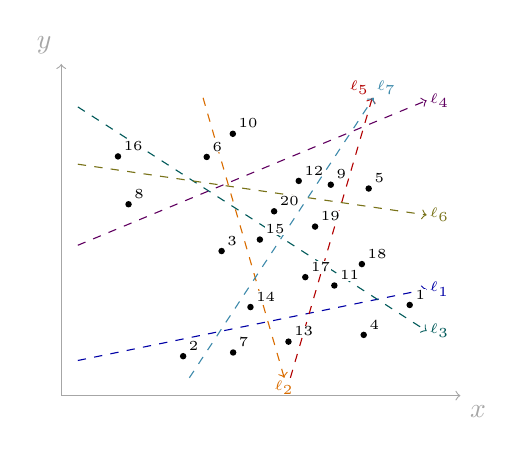
\begin{tikzpicture}[scale=0.78]
  \draw[->,gray!70] (0.45,0.45)--(6.95,0.45) node[below right] {$x$};
  \draw[->,gray!70] (0.45,0.45)--(0.45,5.85) node[above left] {$y$};
  \foreach \i/\linecolor/\xa/\ya/\xb/\yb/\labelanchor in {
    1/blue!65!black/0.72/1.022/6.4/2.182/west,
    2/orange!85!black/2.759/5.3/4.081/0.74/north,
    3/teal!70!black/0.72/5.151/6.4/1.502/west,
    4/violet!75!black/0.72/2.898/6.4/5.256/west,
    5/red!70!black/4.181/0.74/5.515/5.3/south east,
    6/olive!80!black/0.72/4.218/6.4/3.391/west,
    7/cyan!65!black/2.536/0.74/5.536/5.3/south west%
  } {
    \draw[->,color=\linecolor,dashed] (\xa,\ya)--(\xb,\yb);
    \node[anchor=\labelanchor,font=\tiny,text=\linecolor,inner sep=1pt]
      at (\xb,\yb) {$\ell_\i$};
  }
  \foreach \id/\x/\y in {
    1/6.124/1.926, 2/2.435/1.092, 3/3.061/2.804, 4/5.375/1.439,
    5/5.456/3.822, 6/2.819/4.336, 7/3.249/1.152, 8/1.546/3.566,
    9/4.839/3.884, 10/3.244/4.713, 11/4.897/2.243, 12/4.317/3.946,
    13/4.15/1.329, 14/3.531/1.892, 15/3.684/2.991, 16/1.374/4.345,
    17/4.424/2.379, 18/5.345/2.592, 19/4.583/3.202, 20/3.916/3.451
  } {
    \fill[black] (\x,\y) circle (1.5pt);
    \node[anchor=south west,font=\tiny,inner sep=0.4pt,fill=white,
          xshift=1.5pt,yshift=1.5pt] at (\x,\y) {\id};
  }
\end{tikzpicture}
\end{minipage}\hfill
\begin{minipage}[t]{0.60\textwidth}
\vspace{0pt}
\centering
{\small\textbf{One valid decision tree}\par}
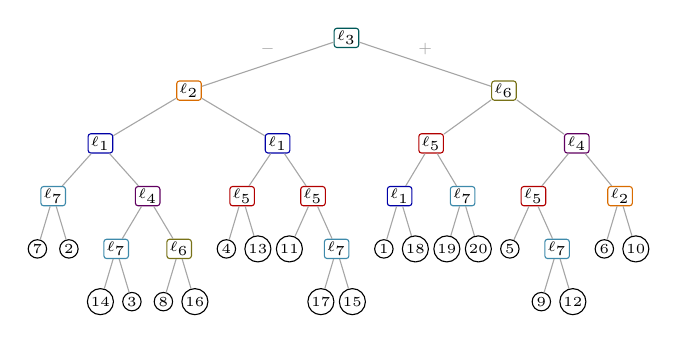
\begin{tikzpicture}[
  x=0.4cm,y=0.67cm,
  query/.style={rounded corners=1pt,fill=white,inner sep=1pt,font=\tiny},
  query1/.style={query,draw=blue!65!black},
  query2/.style={query,draw=orange!85!black},
  query3/.style={query,draw=teal!70!black},
  query4/.style={query,draw=violet!75!black},
  query5/.style={query,draw=red!70!black},
  query6/.style={query,draw=olive!80!black},
  query7/.style={query,draw=cyan!65!black},
  leaf/.style={draw,circle,fill=white,inner sep=0.7pt,font=\tiny},
  edge/.style={gray!70,thin}
]
  \node[query3] (n0) at (9.8125,0) {$\ell_3$};
  \node[query2] (n1) at (4.8125,-1) {$\ell_2$};
  \node[query1] (n2) at (2,-2) {$\ell_1$};
  \node[query7] (n3) at (0.5,-3) {$\ell_7$};
  \node[leaf] (n4) at (0,-4) {7};
  \node[leaf] (n5) at (1,-4) {2};
  \node[query4] (n6) at (3.5,-3) {$\ell_4$};
  \node[query7] (n7) at (2.5,-4) {$\ell_7$};
  \node[leaf] (n8) at (2,-5) {14};
  \node[leaf] (n9) at (3,-5) {3};
  \node[query6] (n10) at (4.5,-4) {$\ell_6$};
  \node[leaf] (n11) at (4,-5) {8};
  \node[leaf] (n12) at (5,-5) {16};
  \node[query1] (n13) at (7.625,-2) {$\ell_1$};
  \node[query5] (n14) at (6.5,-3) {$\ell_5$};
  \node[leaf] (n15) at (6,-4) {4};
  \node[leaf] (n16) at (7,-4) {13};
  \node[query5] (n17) at (8.75,-3) {$\ell_5$};
  \node[leaf] (n18) at (8,-4) {11};
  \node[query7] (n19) at (9.5,-4) {$\ell_7$};
  \node[leaf] (n20) at (9,-5) {17};
  \node[leaf] (n21) at (10,-5) {15};
  \node[query6] (n22) at (14.8125,-1) {$\ell_6$};
  \node[query5] (n23) at (12.5,-2) {$\ell_5$};
  \node[query1] (n24) at (11.5,-3) {$\ell_1$};
  \node[leaf] (n25) at (11,-4) {1};
  \node[leaf] (n26) at (12,-4) {18};
  \node[query7] (n27) at (13.5,-3) {$\ell_7$};
  \node[leaf] (n28) at (13,-4) {19};
  \node[leaf] (n29) at (14,-4) {20};
  \node[query4] (n30) at (17.125,-2) {$\ell_4$};
  \node[query5] (n31) at (15.75,-3) {$\ell_5$};
  \node[leaf] (n32) at (15,-4) {5};
  \node[query7] (n33) at (16.5,-4) {$\ell_7$};
  \node[leaf] (n34) at (16,-5) {9};
  \node[leaf] (n35) at (17,-5) {12};
  \node[query2] (n36) at (18.5,-3) {$\ell_2$};
  \node[leaf] (n37) at (18,-4) {6};
  \node[leaf] (n38) at (19,-4) {10};
  \foreach \parent/\child in {
    n3/n4, n3/n5, n7/n8, n7/n9, n10/n11, n10/n12,
    n6/n7, n6/n10, n2/n3, n2/n6, n14/n15, n14/n16,
    n19/n20, n19/n21, n17/n18, n17/n19, n13/n14, n13/n17,
    n1/n2, n1/n13, n24/n25, n24/n26, n27/n28, n27/n29,
    n23/n24, n23/n27, n33/n34, n33/n35, n31/n32, n31/n33,
    n36/n37, n36/n38, n30/n31, n30/n36, n22/n23, n22/n30%
  } {
    \draw[edge] (\parent)--(\child);
  }
  \draw[edge] (n0)--node[above,font=\tiny] {$-$} (n1);
  \draw[edge] (n0)--node[above,font=\tiny] {$+$} (n22);
\end{tikzpicture}
\end{minipage}
\caption{Seven randomly oriented supplied lines are drawn first, then
twenty hypotheses are placed in distinct cells of their arrangement.
The arrows orient the lines: the positive side is to the left of the
arrow. Each internal node queries the correspondingly colored line.
At every node the left branch is the negative answer and the right
branch is the positive answer. The leaf numbers match the point labels.
This valid tree has maximum depth five.}
\label{fig:problem-example}
\end{figure}

\subsection{Results and the main ideas}

In the restricted results, an all-miss instance has a distinguished
hypothesis that every selected cap misses; its answers form the
all-negative route.

\begin{center}
\small
\begin{tabular}{@{}p{0.45\linewidth}p{0.20\linewidth}p{0.26\linewidth}@{}}
\hline
Setup and objective & Guarantee & Running time\\ \hline
General maximum depth & $<4.464966$ & Polynomial\\
General arbitrary-prior expected depth & $<5.182976$ & Polynomial\\
Either general objective & $2+\varepsilon$ & Quasipolynomial\\
Randomized $\max_h\mathbb E_Td_T(h)$ & $<5.182976$ & Polynomial\\
Same randomized objective & $2+\varepsilon$ & Quasipolynomial\\
All-miss, fixed-size caps: maximum depth & Exact & Polynomial\\
All-miss, weighted singleton/pair paths and cycles: expected depth
 & $1+\varepsilon$ & EPTAS\\
All-miss, uniform fixed-size convex caps: expected depth
 & $1+\varepsilon$ & PTAS\\ \hline
\end{tabular}
\end{center}

Each row reports the strongest guarantee proved for that setup; the
following sections develop the scheduling and coding procedures it
uses.
The expected-depth guarantee permits every strictly positive rational
prior. For $0<\varepsilon\le1$, the general
quasipolynomial algorithms run in
$(mn)^{O(\varepsilon^{-1}\log n)}$ time.

Both exact objectives are strongly NP-complete, including expected
depth under a uniform prior. Constant-factor inapproximability remains
open.

The geometric structure behind the algorithms is easiest to see in a
state (the current set of hypotheses consistent with all answers so
far) where no line splits much of the remaining mass. Every test
then has a majority answer. The opposite, minority half-planes are
small, and Helly's theorem gives a point lying on all majority sides.
After translating this common witness to the origin, each query is
represented by a point in a normalized plane. The vertices of their
convex hull (the smallest convex set containing those points) suffice
to describe the relevant caps: each original cap is covered by at
most two adjacent vertex caps, and the vertex
answers of any one hypothesis form a \emph{circular interval}: a
consecutive block in the cyclic order in which the hull vertices
appear around the polygon, with wrap-around allowed. This turns the
geometric part of the problem into scheduling and searching over
circular intervals.

\paragraph{Maximum depth: schedule discovery against child heights.}
In a flat state, the algorithm first builds the recursive codes for
the hull-pattern classes. It must then discover which class contains
the target, so it schedules positive hull answers with deadlines set
by the child codes' actual heights. To analyze this discovery cost,
follow an optimal tree along the common witness path. If a class stays
on that path through a long prefix, restricting the tree to the class
removes those queries; the saved depth pays for the class's first
positive hull answer in our schedule.

Each original query cap is covered by at most two adjacent hull caps,
so the comparison ordering uses singleton and adjacent-pair blocks.
Enumerating its first adjacent pair fixes a cut and turns the remaining
circular demands into ordinary intervals. The priority scheduler then
preserves the comparison credit at every child-height deadline. When
the number of required discovery ranks is logarithmic, a subset dynamic
program on the spatial Cartesian tree solves the deadline problem in
polynomial time; the recursive bounds show that this logarithmic cap
suffices for the stronger general factor. We charge endpoint recovery
separately. If the witness path already supplies a negative neighboring
answer, the decoder can reuse it to fix one endpoint, leaving a smaller
height allowance for the child code.

\paragraph{Expected depth: pay once for learning a pattern.}
For expected depth, the algorithm again discovers the complete
hull-answer pattern before recursing. The analysis then separates the
cost of finding the pattern from the cost of identifying a hypothesis
inside it. Along an optimal witness path, a class's constant prefix
disappears when the tree is restricted to that class; those saved
queries pay for finding its first positive hull answer. After
discovery, the entropy of the pattern bounds the endpoint information
still unknown. To control discovery cost, we first find the largest
weighted coverage attainable at each integer budget. A finite search
over shifted geometric batches then selects a schedule with a strong
first-cover bound. The endpoint decoder may query one or both endpoints
of a positive block. If it asks both, the second answer provides
information that can shorten later decoding; the adaptive block modes
account for that gain while preserving the individual cap bounds used
in the schedule analysis. Since every adjacent support block has
bounded mass, some targets must wait for later blocks, where the
discrete first-cover estimate gives a sharper charge. The all-negative
route is charged by the waiting time to complete its schedule. Across
the recursive partition, the saved optimal-depth queries and entropy
decreases telescope, so each cost is charged only once.

\paragraph{Strong hardness: encode bin loads by matching choices.}
Both hardness reductions begin with strongly bounded 3-Partition: each
item of size $a_i$ must be assigned to one of $p$ bins, and the target
is load $B$ in every bin. We encode each item's choice by a matching on
its own odd path. The supplied singleton and adjacent-pair queries let
the distinguished hypothesis count first-hit groups along that path;
at the height threshold, the count can attain its lower bound only
when the matching is maximum. Lemma~\ref{lem:odd-path} then identifies
the one unmatched even-position cloud, whose location records the
item's choice. The path gadgets therefore turn a tree attaining the
threshold into a candidate assignment of all items.

We then calibrate the objective so that it tests this assignment.
For maximum depth, cloud sizes control the remaining heights of the
branches. The resulting tail histogram rules out internal unmatched
positions and requires each bin load to be at most $B$; since the loads
sum to $pB$, they must all equal $B$. For expected depth, the matching
cost formula separates a load-independent base cost from a quadratic
penalty in the deviations $L_b-B$, so the chosen threshold accepts
precisely the balanced assignments. These two calculations make the
combinatorial choice visible to the respective objectives. The
integer-parabola construction realizes each singleton, pair, and
private test by an explicit supplied line, completing the geometric
instance. Finally, to obtain the uniform-prior result, we replace a
weight $w$ by $w$ uniform hypotheses and give the new points private
singleton tests. The cost identity adds a common internal
identification term for every matching; because this term does not
depend on the bin choices, the expected-depth comparison and the
reduction are preserved.

\paragraph{Relation to earlier work.}
Karbasi and Zadimoghaddam's constrained binary identification problem
is a close information-theoretic precedent~\cite{karbasi2013}. They
relate unrestricted identification to source coding and study how
query constraints change the search strategy. In our setting, the
common-witness and convex-hull arguments turn the supplied planar
tests into circular-interval demands. Once the hull-answer pattern is
known, entropy measures the
endpoint information still needed to identify the hypothesis, while
coverage accounts for the cost of discovering that pattern. We state
and prove the entropy chain rule, log-sum, and prefix-code bounds used
in this accounting. Cover and Thomas~\cite{ct2006} give broader
background on these information-theoretic tools.

The coverage analysis draws on the first-cover viewpoint in min-sum
set cover. Feige, Lov\'asz, and Tetali charge each element by the rank
of its first covering set~\cite{flt2004}; this is the objective
formalized in Lemma~\ref{lem:mssc}. Gupta, Nagarajan, and Ravi use a
variant of min-sum set cover to approximate optimal expected-cost
decision trees, alongside their work on adaptive TSP~\cite{gupta2017}.
These works provide a
general first-cover accounting model. Our schedulers specialize that
model to weighted circular intervals and exact coverage budgets, then
combine the resulting discovery charge with a separate entropy bound
for endpoint decoding.

Dasgupta's analysis of greedy active learning provides a related
expected-cost comparison: it measures query progress by the probability
mass removed and compares that progress with the cost of an optimal
identification tree~\cite{dasgupta2004}. This mass-removal viewpoint
guides our comparison between pattern-discovery progress and optimal
expected cost. We implement that comparison with first-cover schedules
for circular intervals, then use entropy to account for endpoint
decoding. Adler and Heeringa make a related distinction in their
comparison of decision trees with min-sum set cover: covering the
competitors of an item still leaves the tree responsible for separating
the items it has covered~\cite{adlerheeringa2012}. This separation
supports our two-part accounting for finding a hull-answer class and
identifying its member. Cicalese, Laber, and Saettler study expected and
worst-case costs together for adaptive testing with general query
families~\cite{cicalese2017}; their joint perspective provides context
for the two objectives we analyze under a supplied planar line family.
For hardness context, Chakaravarthy et al. connect
entity-identification trees with min-sum set cover reductions
\cite{chakaravarthy2011}. Our reductions encode matching choices on
odd paths and realize the resulting tests by supplied lines on a
parabola.

There is also a geometric decision-tree precedent. Arkin et al. study
point probes for identifying polygonal models and use a common
intersection point to obtain shallow trees~\cite{arkin1998}. This
common-point method gives geometric context for our witness argument.
Here, Helly's theorem produces the witness after each query is oriented
by its majority side; the convex hull then yields the circular-interval
family used by our schedulers.

\begin{proofstrategy}
\textbf{Reading order.}
\begin{enumerate}
\item Sections~\ref{sec:preliminaries}--\ref{sec:geometry} explain the
      model, restriction credits, and the circular-interval geometry.
\item Sections~\ref{sec:worst}--\ref{sec:scheduling} build the
      deadline and weighted-coverage primitives.
\item Sections~\ref{sec:mass-improvement},
      \ref{sec:quasipolynomial}, and~\ref{sec:polynomial-slots}
      assemble the best general approximation algorithms.
\item Sections~\ref{sec:small-caps}--\ref{sec:uniform-cap-ptas}
      exploit bounded caps. The randomized mixture setup follows,
      in Section~\ref{sec:randomized-programming}, connecting
      expected-depth oracles to mathematical programming.
\item Sections~\ref{sec:boundaries}--\ref{sec:uniform-hardness}
      treat boundary answers and strong NP-completeness.
\end{enumerate}
Each long result first states its supporting propositions and gives
the overall proof. The next subsection proves those propositions.
Construction parameters are calibrated only after the structural argument.
\end{proofstrategy}

\section{Preliminaries and basic accounting}
\label{sec:preliminaries}

We collect the model, coding and information inequalities, and
geometric terminology used by the algorithms. Reduction-specific
graph and complexity definitions are given in
Section~\ref{sec:hardness}.
For a positive integer $r$, write $[r]=\{1,\ldots,r\}$.
The notation $|S|$ denotes set cardinality, while $|Q|$ denotes
the length of a word, vector, or sequence when $Q$ is such an object.
The indicator $\mathbf1[P]$ is one if statement $P$ holds and zero
otherwise. We also write $\mathbf1_A(x)=\mathbf1[x\in A]$ for
the indicator function of a set $A$.
The floor $\lfloor x\rfloor$ and ceiling $\lceil x\rceil$
are the greatest integer at most $x$ and the least integer at least
$x$, respectively. For planar vectors,
$x\cdot y=x_1y_1+x_2y_2$ is the dot product.

\subsection{Line-query model and objectives}

Let $\HH\subset\mathbb R^2$ be $n\ge2$ distinct points. A finite family
$\LL$ of $m$ supplied lines separates every pair of hypotheses,
meaning that every two distinct points receive different answers to
at least one line. Write a line as the zero set of an affine function
$f_\ell(x)=a_\ell\cdot x+b_\ell$, where
$a_\ell\in\mathbb R^2\setminus\{0\}$ and $b_\ell\in\mathbb R$.
Querying $\ell$ returns the sign of $f_\ell(h)$ for
the hidden point $h$. Every query contributes one to the depth.
Unless explicitly stated otherwise, no hypothesis lies on a supplied
line, so the answer is binary.
Section~\ref{sec:boundaries} treats a third, on-line outcome.

After any sequence of queries and answers, the current \emph{state}
is the set of hypotheses whose signs on all queried lines agree with
the answers received. For a state $S$ and a supplied line $\ell$,
write
\[
 S_\ell^-=\{h\in S:f_\ell(h)<0\},\qquad
 S_\ell^+=\{h\in S:f_\ell(h)>0\}.
\]
These are the two answer classes; the line \emph{splits} $S$ when
both classes are nonempty.

\begin{definition}[Line-query decision trees]\label{def:decision-tree}
A binary line-query decision tree is a finite rooted tree whose
internal nodes are labeled by supplied lines and whose two outgoing
edges are labeled by their negative and positive answers. A
hypothesis follows the edge matching its answer at each query.
An \emph{identifying} tree for $S$ has hypothesis labels at its leaves
and sends every $h\in S$ to a leaf labeled $h$. The root has depth
zero; a leaf's depth is the number of queries on its root-to-leaf path,
and the tree's \emph{height} is its largest leaf depth.

A \emph{partial decision tree}, or \emph{stage}, may instead stop at
leaves labeled by nonempty subsets of $S$. Each leaf is labeled by
the hypotheses compatible with its path, so these output
classes partition $S$. Attaching an identifying tree for each class
produces a complete identifying tree.
\end{definition}

We omit a query whenever its answer is already determined by the
current candidate set; in particular, a line is never queried twice
on one path. Thus every internal node of the resulting tree has two
nonempty children, and we call such a tree \emph{proper}. Every
identifying tree can be put in this form by deleting one-child queries
and reusing the already-known answers, so the convention preserves
the optimum. It also gives a useful size bound: if a proper binary tree
on $n$ hypotheses has $I$ internal nodes, edge counting yields
$2I=I+n-1$, hence $I=n-1$ and every path has at most $n-1$ queries.

A \emph{transcript} records the queries and answers observed along
a path. In a fixed binary tree the previous answers determine the
next query, so the transcript can also be represented by its answer
word, encoding negative as $0$ and positive as $1$.
A \emph{cached answer} is an answer already learned on that path;
reusing it or inferring a constant answer costs no additional query.
For nonempty $A\subseteq S$, the \emph{restriction} $T|_A$ is obtained
by deleting leaves outside $A$, deleting empty branches, and
contracting queries with only one surviving outcome. It is a valid
tree on $A$, and no surviving hypothesis's depth increases.

\begin{definition}[Membership answers and spines]\label{def:membership-spine}
A \emph{membership interpretation} designates one answer class $A$
of a supplied binary query. Its answer is a \emph{hit} when $h\in A$
and a \emph{miss} otherwise. A hit may be either affine sign;
interpreting the answer changes neither the supplied line nor its cost.

The \emph{spine} of a distinguished hypothesis is its root-to-leaf
path. Another hypothesis \emph{exits} that path at its first
different answer; the attached subtree is its local exit code.
If this occurs at query position $j$, a local depth $d$ contributes
total depth $j+d$.
If every designated membership set excludes the distinguished
hypothesis, its spine is an all-miss route and exits occur at first hits.
A point $p$ on no supplied line similarly determines a
\emph{witness path}, even when $p\notin\HH$.
\end{definition}

Let $d_T(h)$ be the number of queries on the path followed by $h$,
stopping at its output leaf; for an identifying tree that leaf names $h$.
For a tree $T$ identifying a candidate set $S\subseteq\HH$, define
\[
 c_{\mathrm W}(T)=\max_{h\in S}d_T(h).
\]
For expected depth, let $\pi_h>0$ with $\sum_h\pi_h=1$, write
$w(S)=\sum_{h\in S}\pi_h$, and define
\[
 c_{\mathrm E}(T)=\sum_{h\in S}\pi_h d_T(h).
\]
We retain the original probabilities in $c_{\mathrm E}(T)$ when a tree
identifies a restricted state. Consequently, $c_{\mathrm E}(T)$ is
that state's contribution to the root expectation, while
$c_{\mathrm E}(T)/w(S)$ is its conditional expected cost. At the
root, $w(\HH)=1$, so these quantities agree.
Define the corresponding optima by
\[
 \OPT_{\mathrm W}(S)=\min_{T\text{ identifying }S}c_{\mathrm W}(T),
 \qquad
 \OPT_{\mathrm E}(S)=\min_{T\text{ identifying }S}c_{\mathrm E}(T).
\]
We set both optima to zero on the empty set and on singletons.
Hypothesis weights used later in the hardness proof specify these
probabilities, while query depth still counts each test once. Keeping
weights unnormalized makes the expected costs of disjoint recursive
states add directly.

More explicitly, if positive raw weights $\omega_h$ are supplied,
put $\Omega=\sum_{h\in\HH}\omega_h$ and $\pi_h=\omega_h/\Omega$.
Then, also on a restricted state,
\[
 \sum_{h\in S}\omega_h d_T(h)=\Omega c_{\mathrm E}(T).
\]
Thus normalizing weights divides both a weighted cost and its
decision threshold by the same $\Omega$, leaving the optimal tree
unchanged. The weights determine hypothesis mass in the expected
objective; each query still costs one.

The two objectives now differ only in how they combine the child
states. If $S_\ell^-$ and $S_\ell^+$ are the answer classes in $S$,
their optimality recurrences on nonsingleton states are
\[
 \begin{split}
 \OPT_{\mathrm W}(S)&=1+\min_{\ell\text{ splitting }S}
                    \max\{\OPT_{\mathrm W}(S_\ell^-),
                         \OPT_{\mathrm W}(S_\ell^+)\},\\
 \OPT_{\mathrm E}(S)&=w(S)+\min_{\ell\text{ splitting }S}
                    \{\OPT_{\mathrm E}(S_\ell^-)
                      +\OPT_{\mathrm E}(S_\ell^+)\}.
 \end{split}
\]
Algorithm~\ref{alg:exact-tree} implements these recurrences on the
small local states used later, and the same values serve as benchmarks
for the approximation algorithms. Their different combinations follow
directly from the objectives: a query adds one to every path, so the
maximum-depth recurrence takes the harder child; in expected depth the
query contributes the state's mass $w(S)$, after which the contributions
of the two disjoint child sets add.

\begin{algorithm}[H]
\caption{Exact supplied-query Bellman recursion (small local states)}
\label{alg:exact-tree}
\KwIn{State $S$; objective $o\in\{\mathrm W,\mathrm E\}$; original weights $\pi_h$.}
\KwOut{An optimal supplied-query tree and its cost.}
\If{$|S|\le1$}{\KwRet the leaf of cost zero\;}
\If{the memoized value for $(S,o)$ exists}{\KwRet that value and tree\;}
\ForEach{supplied line $\ell$ splitting $S$}{
  $(T_-,v_-)\gets\ExactTree(S_\ell^-,o)$;
  $(T_+,v_+)\gets\ExactTree(S_\ell^+,o)$\;
  $v_\ell\gets1+\max\{v_-,v_+\}$ if $o=\mathrm W$,
  and $v_\ell\gets w(S)+v_-+v_+$ otherwise\;
}
Memoize the minimum $v_\ell$ and the tree joining its stored children\;
\KwRet the memoized cost and tree\;
\end{algorithm}

Algorithm~\ref{alg:exact-tree} takes $2^{O(|S|)}\operatorname{poly}(m,L)$
time with bit-mask states. Its exponential dependence stays within
bounded local sets, while the approximation algorithms handle larger
states.


All logarithms are natural unless a base is displayed, and
we use $0\ln0=0$, the continuous extension at zero.
Coordinates, line coefficients, and probabilities are rational
and explicitly given by binary-encoded numerators and denominators.
Polynomial time is measured in the total binary encoding length of
this input.
The \emph{decision version} of either objective asks, given an
instance and a threshold $K$, whether a legal identifying tree
has cost at most $K$. For maximum depth the threshold can be
an integer; for expected depth it is rational and the prior is
part of the input.
An \emph{$\alpha$-approximation} for a minimization objective returns
a feasible tree whose cost is at most $\alpha$ times the optimum
on every valid input. For a deterministic algorithm, this bound
applies to the particular tree it returns.
Whenever an algorithm permits several choices, fix a deterministic
tie-breaking rule, such as the input order.

\begin{symboltable}
$\HH,\LL;\ n,m$ & Hypothesis points, supplied lines, and their counts.\\
$S,\ S_\ell^-,S_\ell^+$ & Current state and its negative and positive answer classes for line $\ell$.\\
$d_T(h)$ & Number of queries on the path for hypothesis $h$ in tree $T$.\\
$c_{\mathrm W}(T),\ \OPT_{\mathrm W}(S)$ & Maximum path depth and its minimum over identifying trees for $S$.\\
$\pi_h,\ w(S)$ & Root prior probability of $h$ and the original probability mass of state $S$.\\
$c_{\mathrm E}(T),\ \OPT_{\mathrm E}(S)$ & Expected depth using the original probabilities and its minimum over identifying trees for $S$.\\
$\mathcal E(S)$ & State-mass-weighted entropy of the conditional distribution on $S$.\\
$\Pi,\ \Delta_{\mathrm E}(S,\Pi),\ I(S,\Pi)$ & A partition of $S$, the decrease in optimal expected depth, and the information gained from its class label.\\
$\omega_h,\ \Omega$ & Optional raw positive weights and their total; $\pi_h=\omega_h/\Omega$.\\
\end{symboltable}

\begin{definition}[Balanced and flat states]\label{def:balanced}
Fix $0<\delta<1/3$. A nonsingleton state $S$ is
\emph{count-balanced} if some supplied line has at least
$\delta|S|$ hypotheses on each side. Otherwise it is
\emph{count-flat}. In the flat case, every line has a unique
\emph{majority answer}, on the side containing more than half of $S$.
We call this its \emph{frozen answer} and write $C_\ell$ for the
open half-plane on the opposite side. Its induced answer class
$C_\ell\cap S$ is the \emph{minority cap}, of size less than
$\delta|S|$. We also use ``cap'' for the corresponding half-plane
when discussing its geometry.
\end{definition}

For expected depth, the same split-versus-flat distinction must track
probability mass, since a small number of hypotheses can carry most of
the prior. Accordingly, $S$ is \emph{mass-balanced} if some line has
$w(S_\ell^-),w(S_\ell^+)\ge\delta w(S)$, and \emph{mass-flat}
otherwise. In a mass-flat state, freezing the mass-majority answer
gives $w(C_\ell\cap S)<\delta w(S)$.

To turn each stored object into a legal supplied-query tree, the
procedures use the following conventions. Tables are indexed by
realized hypotheses or patterns, and ties follow input order. During
tree assembly, cached answers supply later virtual questions, the
origin marker records the cut position, and infeasible branches are
discarded. We then contract every query whose answer is constant on
the current state, leaving tests that distinguish hypotheses. The
analysis for each routine gives its parameter values and proves that
they meet the required bounds.



\begin{figure}[htbp]
\centering
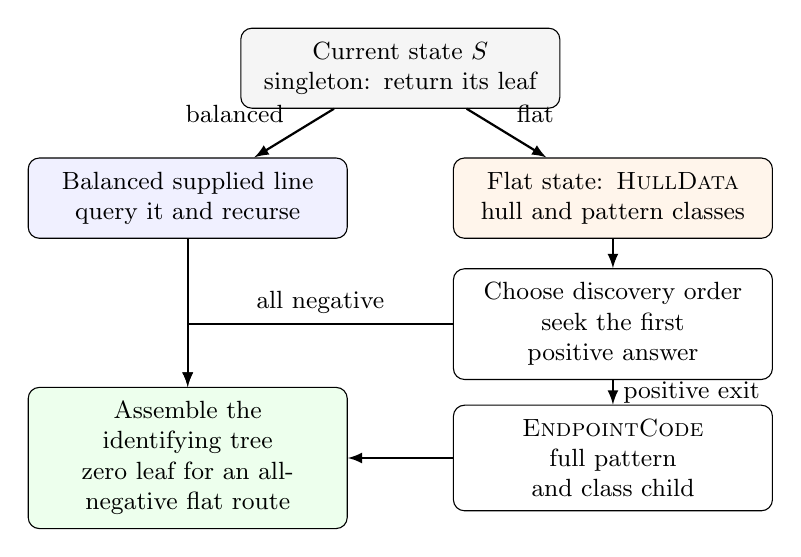
\begin{tikzpicture}[every node/.style={font=\small},
  box/.style={draw,rounded corners,align=center,inner sep=5pt,text width=3.7cm},
  arr/.style={-latex,thick}]
  \node[box,fill=gray!8] (state) at (0,0) {Current state $S$\\singleton: return its leaf};
  \node[box,fill=blue!6] (balanced) at (-2.7,-1.65)
    {Balanced supplied line\\query it and recurse};
  \node[box,fill=orange!8] (flat) at (2.7,-1.65)
    {Flat state: \HullData\\hull and pattern classes};
  \node[box] (discover) at (2.7,-3.25)
    {Choose discovery order\\seek the first positive answer};
  \node[box] (decode) at (2.7,-4.95)
    {\EndpointCode\\full pattern and class child};
  \node[box,fill=green!7] (output) at (-2.7,-4.95)
    {Assemble the identifying tree\\zero leaf for an all-negative flat route};
  \draw[arr] (state) -- node[above left]{balanced} (balanced);
  \draw[arr] (state) -- node[above right]{flat} (flat);
  \draw[arr] (flat) -- (discover);
  \draw[arr] (discover) -- node[right]{positive exit} (decode);
  \draw[arr] (discover.west) -- node[above]{all negative} (-2.7,-3.25)
    -- (output.north);
  \draw[arr] (decode) -- (output);
  \draw[arr] (balanced) -- (output);
\end{tikzpicture}
\caption{The common recursive structure. Arrows show how one stage
feeds the next. For maximum depth, the algorithm constructs class
children first and uses their heights as schedule deadlines. For
expected depth, original prior masses determine the schedule scores.
The flat stage has an all-negative leaf when the zero pattern is
present, and both scheduling and decoding use supplied hull lines.}
\label{fig:recursive-procedure-flow}
\end{figure}




\paragraph{State quantities and calibration choices.}
The state $S$, its mass $w(S)$, pattern classes, and optimal costs
record the instance and the algorithm's progress. Parameters such as
$\delta,\beta,\gamma$ control the constructions; each algorithm states
their admissible conditions before choosing values for its bound. A
coefficient such as $\Phi_\beta$ then records how that calibration and
the current state determine a particular charge.

\begin{proofstrategy}
The accounting facts below have three roles.
\begin{enumerate}
\item Prefix codes turn query transcripts into information lower bounds.
\item Restriction deletes queries that a known output class no longer needs.
\item Potential differences cancel across recursive states, so local
      charges are paid only once.
\end{enumerate}
The statements are collected first. Their proofs appear together in
the next technical subsection, before the geometric terminology.
\end{proofstrategy}

\subsection{Binary codes and ordered comparisons}


\begin{definition}[Binary codes and prefix codes]\label{def:binary-code}
A \emph{binary word} is a finite sequence of bits from $\{0,1\}$;
$\{0,1\}^*$ includes the empty word $\varepsilon$, of length zero.
A \emph{binary code} on a finite nonempty alphabet $\mathcal A$ is
an injective map $c:\mathcal A\to\{0,1\}^*$. The word $c(a)$ is
the \emph{codeword} for $a$, and $\ell_a=|c(a)|$ is its length.
A word $u$ is a \emph{prefix} of $v$ if $v$ starts with all the
bits of $u$. A code is \emph{prefix-free}, or a \emph{prefix code},
if no codeword is a prefix of another distinct codeword.
\end{definition}

For a distribution $(q_a)$ on the alphabet, the code's maximum
length is $\max_a\ell_a$ and its expected length is
$\sum_a q_a\ell_a$.
The prefix tree of a code has one node for each prefix of a
codeword, with the empty prefix at the root and edges appending
$0$ or $1$. For a prefix code its codewords are the leaves,
at depths $\ell_a$. Conversely, the root-to-leaf answer words of
any binary decision tree form a prefix code. Unary nodes, which
have only one child, can be contracted without increasing any depth.
The empty word is permissible only when the alphabet is a singleton.
For example, $c(a)=0$, $c(b)=10$, and $c(c)=11$ form a prefix code
with lengths $1,2,2$.

\begin{definition}[Alphabetic codes]\label{def:alphabetic-code}
For an ordered alphabet $y_1<\cdots<y_r$, a prefix code is
\emph{alphabetic} if its codewords occur in that same lexicographic
order, with $0<1$. An \emph{ordered threshold comparison} asks
whether the unknown outcome is at most $y_j$ for some $j$.
\end{definition}

In an alphabetic prefix tree, the outcomes below each node form
a consecutive range. After unary nodes are contracted, its two
children separate that range at one threshold. Thus an alphabetic
code can be implemented by ordered threshold comparisons whenever
those comparisons are available. The code bits label the two
ordered ranges; a line's raw sign answer is routed to the matching
range, even if its sign encoding uses the opposite bit. Relabeling
therefore only changes the names of the two outcomes. Kraft's
inequality applies to every prefix
code, while an executable decision-tree code must also use comparisons
available in the supplied line family. Section~\ref{sec:endpoint-geometry}
verifies that the endpoint-code comparisons meet this condition.

A word $b_1\cdots b_\ell$ specifies the half-open \emph{dyadic cell}
\[
 D(b_1\cdots b_\ell)=
 \left[\sum_{j=1}^{\ell}b_j2^{-j},
       \sum_{j=1}^{\ell}b_j2^{-j}+2^{-\ell}\right)
 \subseteq[0,1).
\]
The empty word specifies $[0,1)$. Such cells are nested or disjoint;
one word is a prefix of another if and only if its cell contains
the other's cell. Half-open endpoints avoid ambiguity at dyadic
rationals.

Query transcripts occupy disjoint leaves of a binary code. The next
inequality expresses their limited capacity; it will turn leaf depths
into lower bounds on both decision-tree objectives.

\begin{theorem}[Kraft's inequality for binary prefix codes]
\label{thm:kraft}
Every finite binary prefix code has lengths satisfying
\[
 \sum_{a\in\mathcal A}2^{-\ell_a}\le1.
\]
Conversely, nonnegative integer lengths $(\ell_a)_{a\in\mathcal A}$
are realizable by a binary prefix code if this inequality holds.
The converse specifies codeword lengths; alphabetic order and
implementation by a restricted query family require additional
structure.
\end{theorem}


The code $0,10,11$ has Kraft sum
$2^{-1}+2^{-2}+2^{-2}=1$. More generally, equality holds for a
proper binary tree because its two child cells partition each
internal node's cell. The coding facts here and the information
inequalities below are standard; see Cover and Thomas~\cite{ct2006}.

\subsection{Entropy and information inequalities}

\begin{definition}[Entropy and conditional entropy]\label{def:entropy}
A \emph{probability vector} $(q_i)$ has nonnegative entries summing
to one; its \emph{support} consists of the indices with $q_i>0$.
For a finite random variable $Y$ with probabilities
$q_y=\Pr[Y=y]$, its Shannon entropy in natural-log units is
\[
 H(Y)=-\sum_y q_y\ln q_y.
\]
We also write $H(q)$ for the entropy of a probability vector.
The joint entropy $H(Y,Z)$ is the entropy of the pair $(Y,Z)$.
For $Z$ with finite support, conditional entropy is
\[
 H(Y\mid Z)=
 \sum_{z:\Pr[Z=z]>0}\Pr[Z=z]\,H(Y\mid Z=z),
\]
where the inner entropy uses
$\Pr[Y=y\mid Z=z]=\Pr[Y=y,Z=z]/\Pr[Z=z]$.
Conditioning on several variables means
conditioning on their tuple. Entropy in bits is $H(Y)/\ln2$.
For a function $g$ of a finite random variable,
$\mathbb E[g(Y)]=\sum_y q_y g(y)$.
The \emph{binary entropy} is
$h(t)=-t\ln t-(1-t)\ln(1-t)$ for $0\le t\le1$.
We write $H_2(t)=h(t)/\ln2$ when binary entropy is measured in bits.
\end{definition}

For nonempty $S$, the conditional hypothesis probabilities are
$q_h=\pi_h/w(S)$. Define the \emph{weighted state entropy} by
\[
 \mathcal E(S)=w(S)H(q)
       =\sum_{h\in S}\pi_h\ln\frac{w(S)}{\pi_h},
 \qquad \mathcal E(\varnothing)=0.
\]
It is zero on singletons. Like $c_{\mathrm E}$, this quantity
retains the original state mass.

To lower-bound average depth, we compare hypothesis probabilities
with the capacities assigned to their codewords. Log-sum makes this
comparison without any assumption on the smallest probability.

\begin{lemma}[Log-sum inequality]\label{lem:log-sum}
For nonnegative $a_i$ and positive $b_i$, with
$A=\sum_i a_i>0$ and $B=\sum_i b_i$, one has
\[
 \sum_i a_i\ln\frac{a_i}{b_i}\ge A\ln\frac AB,
\]
with zero summands interpreted by continuity.
\end{lemma}


A stage first reveals a pattern and then identifies the hypothesis
within that pattern. Since the pattern is a function of the hypothesis,
the entropy chain rule separates the information spent on these two
tasks. This separation lets the later endpoint decoder pay only for
the information left after pattern discovery.

\begin{lemma}[Entropy chain rule]\label{lem:entropy-chain-rule}
For finite random variables,
\[
 H(Y,Z)=H(Z)+H(Y\mid Z),\qquad
 H(Y,Z\mid W)=H(Y\mid W)+H(Z\mid Y,W).
\]
If $Z$ is determined by $Y$, then
$H(Y)=H(Z)+H(Y\mid Z)$. Also,
$0\le H(Y)\le\ln|\operatorname{supp}(Y)|$ and
$H(Y\mid Z)\ge0$; in particular $0\le h(t)\le\ln2$.
\end{lemma}


An information-efficient code must also respect the queries we can
ask. For ordered endpoint outcomes, alphabetic codes keep each branch
consecutive and therefore make the coding bound executable by thresholds.

\begin{lemma}[Alphabetic threshold codes]\label{lem:alphabetic-endpoints}
Let $Y$ have finite ordered support, and let $H(Y)$ be its entropy
with natural logarithms. There is an explicit alphabetic threshold
code with depth on outcome $y$ at most
$\log_2(1/\Pr[Y=y])+2$.
In particular its expected depth is at most
\[
 \frac{H(Y)}{\ln2}+2.
\]
This is a dyadic prefix-code construction; see Cover and
Thomas~\cite{ct2006} for the general coding background. The short
proof here also verifies the extra alphabetic (order-preserving)
property needed for threshold queries.
An optimal expected-depth threshold tree can also be computed by
a polynomial interval dynamic program. The explicit code is used
when the pointwise depth bound is needed.
\end{lemma}
\begin{proof}[Proof of Lemma~\ref{lem:alphabetic-endpoints}]
Claims~\ref{clm:alphabetic-1} and~\ref{clm:alphabetic-2} construct
the stated executable code; averaging its pointwise bound proves
the expected-depth inequality. Claim~\ref{clm:alphabetic-3} gives
the optimal threshold-tree algorithm.
\end{proof}


\begin{algorithm}[H]
\caption{Alphabetic code on ordered outcomes}
\label{alg:alphabetic-code}
\KwIn{Ordered outcomes $y_1<\cdots<y_r$ of positive rational masses $a_i$;
mode \emph{pointwise} or \emph{expected}.}
\KwOut{A threshold-comparison tree.}
\If{$r=1$}{\KwRet its zero-depth leaf\;}
\eIf{mode is \emph{pointwise}}{
  Normalize $q_i=a_i/\sum_j a_j$ and put $F_i=\sum_{j<i}q_j$\;
  \ForEach{$i$}{
    Find $d_i=\lceil\log_2(1/q_i)\rceil+1$ by rational powers-of-two comparisons\;
    Take the depth-$d_i$ dyadic cell containing $F_i+q_i/2$ as codeword $i$\;
  }
  Build the alphabetic prefix tree and contract unary nodes\;
}{
  Set $D_{i,i}=0$\;
  \For{$h=2,\ldots,r$}{
    \ForEach{$[i,j]$ of length $h$}{
      $D_{i,j}\gets\sum_{a=i}^j a_a+min_{i\le t<j}(D_{i,t}+D_{t+1,j})$\;
      Store a minimizing split after $y_t$\;
    }
  }
  Reconstruct the stored interval splits\;
}
\KwRet the ordered tree, implementing each split by its available threshold\;
\end{algorithm}

The pointwise mode preserves the per-outcome bound; the expected mode
has $O(r^3)$ arithmetic complexity and avoids long expansions for small
priors. Their distinct roles are proved in
Lemma~\ref{lem:alphabetic-endpoints}.


\subsection{Restriction and recursive accounting}

The next accounting step separates two sources of progress. Once a
class is known, restriction contracts queries that no longer help
identify its members; meanwhile, the class label itself carries
information measured by entropy. These give complementary lower bounds
for the work performed by a stage.

\begin{definition}[Partitions and refinement]\label{def:partitions}
A \emph{partition} $\Pi$ of $S$ is a family of pairwise disjoint
nonempty subsets whose union is $S$. We say $\Pi$ \emph{refines}
$\mathcal R$, or $\mathcal R$ is \emph{coarser} than $\Pi$, if
every class of $\Pi$ is contained in a class of $\mathcal R$.
The output classes of a partial decision tree form a partition.
\end{definition}

Revealing an output class can only make identification easier: queries
whose answers are then known disappear. This observation compares
recursive optima, while the coding inequalities provide a lower bound
on how much work any identifying tree still requires.

\begin{lemma}\label{lem:restriction}
For pairwise disjoint subsets $S_1,\ldots,S_k$ of a state $S$,
\[
 \sum_i \OPT_{\mathrm E}(S_i)\le \OPT_{\mathrm E}(S),\qquad
 \OPT_{\mathrm W}(S_i)\le \OPT_{\mathrm W}(S).
\]
Moreover,
\[
 \OPT_{\mathrm E}(S)\ge\frac{\mathcal E(S)}{\ln2},
 \qquad
 \OPT_{\mathrm W}(S)\ge\frac{\ln|S|}{\ln2}
 \quad\text{for nonempty }S.
\]
\end{lemma}
\begin{proof}[Proof of Lemma~\ref{lem:restriction}]
Claim~\ref{clm:restriction-1} gives both restriction inequalities.
Claims~\ref{clm:restriction-2} and~\ref{clm:restriction-3} supply
the two information lower bounds.
\end{proof}


We use the word \emph{potential} for a state quantity that measures
remaining work. Here the relevant expected-depth potentials are
$\OPT_{\mathrm E}$ and $\mathcal E$. When a partition is revealed, its
decrement is the parent value minus the sum of the child values.
For a nonempty state $S$ and a partition $\Pi$ of it, write
\[
 \begin{split}
  \Delta_{\mathrm E}(S,\Pi)&=\OPT_{\mathrm E}(S)
                     -\sum_{A\in\Pi}\OPT_{\mathrm E}(A),\\
  I(S,\Pi)&=\mathcal E(S)-\sum_{A\in\Pi}\mathcal E(A)
           =\sum_{A\in\Pi}w(A)\ln\frac{w(S)}{w(A)}.
  \end{split}
 \]
  Let $X$ be a random hypothesis with
 $\Pr[X=h]=\pi_h/w(S)$, and let $P$ be its class label under $\Pi$.
 Then
 \[
  I(S,\Pi)=w(S)H(P),\qquad
  H(P)=-\sum_{A\in\Pi}\frac{w(A)}{w(S)}
                          \ln\frac{w(A)}{w(S)}.
 \]
Thus $I(S,\Pi)$ is the state mass times the Shannon entropy of the
class label, measured in natural-log units; this is the partition
form of the chain rule in Lemma~\ref{lem:entropy-chain-rule}.
Lemma~\ref{lem:restriction} shows that
$\Delta_{\mathrm E}(S,\Pi)\ge0$, since revealing the class cannot
increase the optimal expected cost. The entropy interpretation gives
$I(S,\Pi)\ge0$ as well. The two quantities therefore measure distinct
credits from the same stage: the decrease in optimal cost and the
information in its class label. The approximation proofs bound stage
costs by these credits, and the cancellation below shows that summing
them over the recursion charges each root-level potential only once.

\begin{proofstrategy}
Sum each potential decrement over the recursive partition tree; every
nonroot state then cancels once as a child against once as a parent.
Singleton leaves have zero potential, and the stage-cost bound can be
summed because each query's original-probability cost is assigned to
a unique stage.
\end{proofstrategy}

\begin{proposition}[Local charges add to a global bound]
\label{prop:potential-cancellation}
Suppose a recursive partition ends in singletons, and its stage at
state $S$ costs at most
$a\Delta_{\mathrm E}(S,\Pi_S)+cI(S,\Pi_S)$.
The complete tree then has expected cost at most
$a\OPT_{\mathrm E}(\HH)+c\mathcal E(\HH)$.
\end{proposition}
\begin{proof}
For either potential $P=\OPT_{\mathrm E}$ or $P=\mathcal E$, sum
over the internal state occurrences in the recursive partition tree.
Every nonroot internal state occurs once as a child and once as a
parent. Therefore
\[
\begin{aligned}
 \sum_{S\ {\rm internal}}
       \left(P(S)-\sum_{A\in\Pi_S}P(A)\right)
 &=P(\HH)-\sum_{A\ {\rm leaf}}P(A)\\
 &=P(\HH).
\end{aligned}
\]
The second equality uses the singleton leaves, where both potentials
are zero. Because state costs retain the original probabilities,
each query's weighted contribution belongs to a unique stage.
Writing $W(S)$ for that stage contribution gives
\[
\begin{aligned}
 c_{\mathrm E}(T)
 &=\sum_{S\ {\rm internal}}W(S)\\
 &\le a\sum_{S\ {\rm internal}}\Delta_{\mathrm E}(S,\Pi_S)
       +c\sum_{S\ {\rm internal}}I(S,\Pi_S)\\
 &=a\OPT_{\mathrm E}(\HH)+c\mathcal E(\HH),
\end{aligned}
\]
as required.
\end{proof}

\subsection{Proofs of the coding and accounting facts}

\begin{proof}[Proof of Theorem~\ref{thm:kraft}]
For necessity, prefix-free codewords specify disjoint dyadic cells
inside $[0,1)$, whose widths are $2^{-\ell_a}$. Summing their
widths therefore gives at most the width one of the containing
interval, which is the required inequality.

For sufficiency, reorder the lengths as
$\ell_1\le\cdots\le\ell_r$ and put
$s_i=\sum_{j<i}2^{-\ell_j}$. Each $s_i$ is an integer multiple
of $2^{-\ell_i}$ because every earlier length is at most $\ell_i$:
the ratio $2^{-\ell_j}/2^{-\ell_i}=2^{\ell_i-\ell_j}$ is an
integer. The intervals $[s_i,s_i+2^{-\ell_i})$ are dyadic cells
of the prescribed depths. They are disjoint and lie in $[0,1)$
by the assumed bound. Their binary descriptions give the required
prefix code; assign them back to the original symbols.
\end{proof}

\begin{proof}[Proof of Lemma~\ref{lem:log-sum}]
Put $q_i=a_i/A$ and $r_i=b_i/B$.
The inequality $-\ln x\ge1-x$ for $x>0$ follows because
$x-1-\ln x$ has its minimum zero at $x=1$. Hence
\[
 \sum_{i:q_i>0}q_i\ln\frac{q_i}{r_i}
 \ge\sum_{i:q_i>0}(q_i-r_i)
 =1-\sum_{i:q_i>0}r_i\ge0.
\]
Here the first step applies that scalar inequality to $x=r_i/q_i$
and multiplies by $q_i$; the equality uses $\sum_iq_i=1$,
and the final step uses $\sum_ir_i=1$ and $r_i\ge0$.
Since $a_i/b_i=(A/B)(q_i/r_i)$ on the positive support,
multiplying by $A$ and adding $A\ln(A/B)$ proves the assertion.
\end{proof}

\begin{proof}[Proof of Lemma~\ref{lem:entropy-chain-rule}]
Write $p_z=\Pr[Z=z]$ and $q_{y\mid z}=\Pr[Y=y\mid Z=z]$ for
$p_z>0$. Zero-probability events contribute zero. Expanding
the logarithm in the joint entropy gives
\[
\begin{aligned}
 H(Y,Z)
 &=-\sum_{z:p_z>0}\sum_y p_zq_{y\mid z}
                           (\ln p_z+\ln q_{y\mid z})\\
 &=-\sum_z p_z\ln p_z\sum_yq_{y\mid z}
       +\sum_zp_z\left(-\sum_yq_{y\mid z}\ln q_{y\mid z}\right)\\
 &=H(Z)+H(Y\mid Z),
\end{aligned}
\]
because each conditional distribution sums to one.
Under $W=w$, apply the same identity with $Y$ first:
$H(Y,Z\mid W=w)=H(Y\mid W=w)+H(Z\mid Y,W=w)$.
Multiplying by $\Pr[W=w]$ and summing gives the conditional form.
If $Z$ is determined
by $Y$, the pair $(Y,Z)$ has the same entropy as $Y$.
Entropy and conditional entropy are nonnegative because their
summands are $-q\ln q\ge0$ for $q\in[0,1]$.
If $r=|\operatorname{supp}(Y)|$, apply Lemma~\ref{lem:log-sum}
with $a_y=q_y$
and $b_y=1/r$ on that support. Since both sums equal one,
\[
 0\byref{Lem.}{lem:log-sum}{\le}\sum_yq_y\ln(rq_y)=\ln r-H(Y),
\]
where the equality separates $\ln(rq_y)=\ln r+\ln q_y$
and uses $\sum_yq_y=1$. This proves the upper bound; applying
it to a binary variable also gives $h(t)\le\ln2$.
\end{proof}

\begin{proofstrategy}
For Lemma~\ref{lem:alphabetic-endpoints}, place a small dyadic cell
inside each probability interval. Disjoint cells preserve outcome
order; their depths give the coding bound. A separate interval
recurrence optimizes the executable threshold tree.
\end{proofstrategy}

\begin{claim}[Ordered disjoint cells give an alphabetic code]
\label{clm:alphabetic-1}
Each outcome's cumulative-probability interval contains a dyadic
cell. These cells are disjoint, occur in outcome order, and form
an alphabetic prefix code.
\end{claim}
\begin{proof}
For an ordered outcome $y$ of probability $a$, let
$F_y=\sum_{y'<y}\Pr[Y=y']$. Its \emph{cumulative-probability
interval} is $[F_y,F_y+a)$, with midpoint $m_y=F_y+a/2$.
The \emph{midpoint-dyadic code} chooses the dyadic cell containing
$m_y$ at depth $\ell_y=\lceil\log_2(2/a)\rceil$, in the sense
of the cells defined before Theorem~\ref{thm:kraft}.
If $s_y$ is the cell's left endpoint and $w_y=2^{-\ell_y}$ its
width, then $s_y\le m_y<s_y+w_y$ and $w_y\le a/2$. Therefore
\[
 s_y>m_y-w_y\ge F_y,\qquad
 s_y+w_y\le m_y+w_y\le F_y+a.
\]
The strict first inequality follows from $m_y<s_y+w_y$;
both outer interval bounds then use $w_y\le a/2$ and
$m_y=F_y+a/2$. Consequently no cell reaches outside its own
probability interval, even when a midpoint is dyadic.
Thus the entire half-open cell lies in $[F_y,F_y+a)$.
These cells are disjoint and appear in
outcome order. Their binary descriptions form a prefix-free
alphabetic code. 
\end{proof}

The cells have given an abstract ordered code. We now check that its
branches are legal threshold comparisons and that converting the code
to a tree preserves the promised depth.

\begin{claim}[Threshold implementation preserves the depth bound]
\label{clm:alphabetic-2}
Ordered threshold queries implement the code with depth at most $\log_2(1/\Pr[Y=y])+2$ on outcome $y$.
\end{claim}
\begin{proof}
By Claim~\ref{clm:alphabetic-1}, outcome $y$ has a codeword of
length $\lceil\log_2(2/a)\rceil$, where $a=\Pr[Y=y]$.
Since $\lceil x\rceil\le x+1$, these lengths
satisfy
\[
 \left\lceil\log_2\frac2a\right\rceil
 \le\log_2\frac1a+2.
\]
After unary nodes are contracted, each internal node separates
two consecutive outcome ranges and is a threshold comparison,
as explained after Definition~\ref{def:alphabetic-code}.
Contraction only decreases depth. Thus taking expectation of the
pointwise bound gives an expected depth at most
\[
 \sum_y\Pr[Y=y]\left(\log_2\frac1{\Pr[Y=y]}+2\right)
 =\frac{H(Y)}{\ln2}+2.
\]
The equality uses the definition of entropy and the fact that the
outcome probabilities sum to one.
\end{proof}

The explicit code supplies a bound for each outcome. When only average
depth matters, the consecutive ranges also admit an exact optimization
that avoids constructing long codewords for very small probabilities.

\begin{claim}[An interval recurrence minimizes expected depth]
\label{clm:alphabetic-3}
Optimal expected-depth threshold comparison uses a polynomial interval dynamic program.
\end{claim}
\begin{proof}
To minimize expected depth, let $D_{i,j}$ be the minimum weighted
depth contributed by outcomes $y_i,\ldots,y_j$, using their original
probabilities $p_a=\Pr[Y=y_a]$. Set $D_{i,i}=0$. For $i<j$, a root
threshold after $y_t$ contributes $\sum_{a=i}^j p_a$, so
\[
 D_{i,j}=\sum_{a=i}^j p_a+
       \min_{i\le t<j}\{D_{i,t}+D_{t+1,j}\}.
\]
Indeed, every outcome in the interval pays for the root query;
the two disjoint child intervals then contribute their optimal
weighted costs. Conversely, every legal threshold root has one of
these split positions, so minimizing over $t$ is exact.
This interval dynamic program uses $O(r^3)$ arithmetic operations.
The resulting optimal alphabetic tree satisfies the
expected-depth bound of Claim~\ref{clm:alphabetic-2}, since that
claim supplies a feasible comparison tree. Thus the interval program
optimizes average depth, while the explicit midpoint-dyadic
construction supplies the pointwise depth bound.
\end{proof}



\begin{proofstrategy}
For Lemma~\ref{lem:restriction}, contract known-answer queries to
obtain feasible subproblem trees. Then use the prefix transcripts in
two ways: Kraft and log-sum bound average depth; the number of binary
leaves bounds maximum depth.
\end{proofstrategy}

\begin{claim}[Restriction cannot increase depth]
\label{clm:restriction-1}
Restriction to pairwise disjoint sets cannot increase their total expected optimum or any maximum-depth optimum.
\end{claim}
\begin{proof}
Restrict an optimal tree on $S$ to each $S_i$ and contract its constant
queries. No hypothesis's depth increases. For an expected-depth
optimal tree $T$, feasibility of each restriction, disjointness,
and nonnegative weights give, in order,
\[
\begin{aligned}
 \sum_i\OPT_{\mathrm E}(S_i)
 &\le\sum_i\sum_{h\in S_i}\pi_hd_{T|_{S_i}}(h)\\
 &\le\sum_i\sum_{h\in S_i}\pi_hd_T(h)
   =\sum_{h\in\bigcup_iS_i}\pi_hd_T(h)\\
 &\le\sum_{h\in S}\pi_hd_T(h)=\OPT_{\mathrm E}(S).
\end{aligned}
\]
For a maximum-depth-optimal tree $T_W$ and nonempty $S_i$,
\[
 \OPT_{\mathrm W}(S_i)
 \le\max_{h\in S_i}d_{T_W|_{S_i}}(h)
 \le\max_{h\in S_i}d_{T_W}(h)
 \le\max_{h\in S}d_{T_W}(h)=\OPT_{\mathrm W}(S).
\]
Here feasibility bounds the optimum by the restricted height,
contraction bounds that height by the original depths on $S_i$,
and inclusion $S_i\subseteq S$ bounds those depths by the full
height. Thus the same restriction operation proves both objectives'
monotonicity.
Empty subsets have optimum zero by convention.


\end{proof}

Restriction preserves a feasible tree on each subproblem. To quantify
the cost of those trees, the next claim turns their transcripts into a
lower bound that depends on the prior.

\begin{claim}[Entropy lower-bounds expected cost]
\label{clm:restriction-2}
Every identifying tree has expected cost at least $\mathcal E(S)/\ln2$.
\end{claim}
\begin{proof}
For entropy, assume $S\ne\varnothing$; the empty-state case is
immediate. Let $q_h=\pi_h/w(S)$. The leaf transcripts are a binary
prefix code as in Definition~\ref{def:binary-code}: a transcript
cannot continue beyond a leaf. Theorem~\ref{thm:kraft} therefore
gives $\sum_h2^{-\ell_h}\le1$ for their lengths.
Apply Lemma~\ref{lem:log-sum}, dividing by $\ln2$ to use base two, with
$\ell_h=d_T(h)$ and $q_h=\pi_h/w(S)$:
\[
 \begin{aligned}
 \sum_h q_h\ell_h-\sum_hq_h\log_2\frac1{q_h}
 &=\sum_hq_h\log_2\frac{q_h}{2^{-\ell_h}}\\
 &\byref{Lem.}{lem:log-sum}{\ge}\log_2\frac{\sum_hq_h}{\sum_h2^{-\ell_h}}
 \byref{Thm.}{thm:kraft}{\ge}0.
 \end{aligned}
\]
The first inequality is the log-sum inequality, and the second uses
$\sum_hq_h=1$ and Kraft's bound. Hence every tree identifying $S$
satisfies
\[
 c_{\mathrm E}(T)=w(S)\sum_hq_hd_T(h)
 \ge w(S)\sum_hq_h\log_2\frac1{q_h}
 =\frac{w(S)}{\ln2}\sum_hq_h\ln\frac1{q_h}
 =\frac{\mathcal E(S)}{\ln2}.
\]
The inequality is the preceding code-length bound multiplied by
$w(S)$; the last equality is the definition of weighted state
entropy. Minimizing over identifying trees therefore gives the
expected-depth lower bound.

\end{proof}

For maximum depth, probabilities are irrelevant. Counting the leaves
that fit within a given height gives the corresponding lower bound.

\begin{claim}[Binary capacity lower-bounds height]
\label{clm:restriction-3}
A binary tree of height $d$ has at most $2^d$ leaves, so identifying $S$ requires height at least $\log_2|S|$.
\end{claim}
\begin{proof}
For the maximum-depth bound, prove by induction on $d$ that a binary
tree of height $d$ has at most $2^d$ leaves. The claim is immediate
for $d=0$; for $d>0$, the root has at most two child subtrees, each
of height at most $d-1$, so together they have at most
$2\cdot2^{d-1}=2^d$ leaves. Thus $|S|\le2^d$, or
$d\ge\log_2|S|=\ln|S|/\ln2$.
\end{proof}



\subsection{Convex geometry and finite set systems}

\begin{definition}[Planar convexity]\label{def:convex-geometry}
A set is \emph{convex} if it contains the segment joining any two
of its points. A \emph{convex combination} is a sum
$\sum_j\lambda_j u_j$ with $\lambda_j\ge0$ and
$\sum_j\lambda_j=1$. The \emph{convex hull}
$\operatorname{conv}(U)$ of a finite nonempty point set $U$ is the set of
its convex combinations. A \emph{vertex}, or extreme point, cannot
be expressed as a convex combination of other points of the hull.
The hull is the convex hull of its vertices; set
$\operatorname{conv}(\varnothing)=\varnothing$ by convention.

A nonempty planar hull has affine dimension zero, one, or two according
as it is a point, a nontrivial segment, or has nonempty planar
interior. In dimension two it is a convex polygon, whose vertices
have a cyclic boundary order; its \emph{edges} join consecutive
vertices. A \emph{supporting line} meets a convex set and leaves
it entirely on one closed side. It \emph{exposes} a point if that
point is its unique intersection with the set. A finite point
set is in \emph{strictly convex position} if every point is a
vertex of its hull.
\end{definition}

An open half-plane has the form $\{x:a\cdot x>b\}$ for $a\ne0$;
replacing $>$ by $\ge$ gives its closed counterpart. A point is
\emph{strictly} on a chosen side when it lies in that side's open
half-plane. A common strict \emph{witness} for several chosen sides
lies in all their open half-planes and may be any point in the plane.

The geometry will produce witnesses for every three majority sides.
The planar Helly theorem is the step that turns this local consistency
into a single witness for all supplied lines.

\begin{theorem}[Planar Helly theorem]\label{thm:helly}
If every subfamily of at most three
sets in a finite family of planar convex sets has nonempty
intersection, then the whole family has nonempty intersection.
The sets may be open.
\end{theorem}
This is the standard planar form; see Matou\v{s}ek~\cite{matousek2002}.

\begin{definition}[Covers and hitting sets]\label{def:covers-and-hitting}
A finite \emph{set system} consists of a universe $U$, a candidate
set $V$, and supplied subsets $F_v\subseteq U$ indexed by $v\in V$.
A \emph{cover} of $U$ is a choice of these sets whose union contains
every element of $U$.
In the equivalent demand formulation, there is a candidate set $V$
and a subset $D_h\subseteq V$ for each demand $h$. A \emph{hitting
set} is a subset $P\subseteq V$ with $P\cap D_h\ne\varnothing$
for every demand. Choosing $v$ covers the set
$F_v=\{h:v\in D_h\}$. Thus covering demands by candidates and
hitting their subsets are the same incidence problem.
A demand with $D_h=\varnothing$ is uncoverable.
\end{definition}

With positive demand weights, a choice covers the sum of the weights
of the demands it hits, counting each demand once. An
\emph{incidence table} records the bits
$\mathbf1[h\in F_v]$, equivalently $\mathbf1[v\in D_h]$.
A cardinality budget is a nonnegative integer $k$ permitting at
most $k$ selected candidates. We may cap it at $|V|$, since there
are no more distinct candidates to choose.

\begin{definition}[Ordered and circular intervals]\label{def:ordered-intervals}
On a finite linear order $v_1,\ldots,v_M$, an \emph{ordinary
interval} is a consecutive subset $\{v_i,\ldots,v_j\}$; we also
allow the empty interval. Its nonempty intervals have first and
last elements, called their endpoints.
On a cyclic order, a \emph{circular interval} is a consecutive
block with wrap-around allowed, also permitting the empty and
whole-cycle sets. Two vertices are \emph{adjacent} when consecutive
in this order, including $v_M,v_1$ on a cycle. An \emph{oriented
adjacent pair} specifies which of those two vertices is first.
A \emph{run} of $P$ in a linear candidate order is a maximal
nonempty consecutive block contained in $P$; $c(P)$ counts such
runs, with $c(\varnothing)=0$.
\end{definition}

Cutting a cyclic order at a removed vertex turns any circular
interval avoiding that vertex into an ordinary interval.
When interval demands occur below, candidates are the ordered
vertices, and selecting any vertex in a demand's interval hits it.

\subsection{Query orderings and first-cover costs}

Let a universe $U$ have positive element weights $\pi_h$ and supplied
sets $F_v$ covering $U$. We allow these weights to be unnormalized.
A \emph{cover ordering}
$Q=(F_{v_1},\ldots,F_{v_\ell})$ is a sequence of distinct supplied
sets whose union covers $U$, and $|Q|=\ell$ is its length.
The \emph{first-cover time}, or \emph{latency}, of $h$ is
$t_Q(h)=\min\{j:h\in F_{v_j}\}$.
The \emph{weighted min-sum set cover} objective is
\[
 \MSSC(Q)=\sum_{h\in U}\pi_h t_Q(h).
\]
Equivalently, $\MSSC(Q)$ is the sum of the uncovered mass before
each step: a demand first covered at position $t_Q(h)$ contributes
its weight to the residuals at positions
$0,\ldots,t_Q(h)-1$. Interchanging these finite sums gives
\[
 \MSSC(Q)=
 \sum_{j=0}^{|Q|-1}
 w\left(U\setminus\bigcup_{r=1}^{j}F_{v_r}\right),
 \qquad w(E)=\sum_{h\in E}\pi_h.
\]
The union for $j=0$ is empty. \emph{Maximum-remaining-weight greedy}
repeatedly chooses the supplied set containing the largest total
weight of elements not yet covered, counting each element only once.

\subsection{Normalized queries and hull patterns}

\begin{definition}[Witness-relative query notation]\label{def:normalized-queries}
Enumerate the supplied lines as $\ell_1,\ldots,\ell_m$.
For a state $S$ and a point $p$ on no supplied line, put
\[
 x_h=h-p,\qquad
 u_i=-\frac{a_{\ell_i}}{f_{\ell_i}(p)},\qquad
 C_i=\{y:u_i\cdot(y-p)>1\}.
\]
Thus $x_h$ is a translated hypothesis vector, $u_i$ a normalized
query vector, and $C_i$ the cap opposite $p$ in the original plane.
The corresponding dual demand is
\[
 R_h=\{u:u\cdot x_h>1\}.
\]
Write $K=\operatorname{conv}(\{0\}\cup\{u_i:i\in[m]\})$ and let
$V$ be its nonzero vertices, in cyclic hull order.
Every $v\in V$ equals a supplied query vector; choose one
representative line if several coincide, and put
$C_v=\{y:v\cdot(y-p)>1\}$.
A \emph{support block} $J_i\subseteq V$ represents $u_i$ as
$u_i=\sum_{v\in J_i}\alpha_{iv}v$, with positive coefficients
and $\sum_v\alpha_{iv}\le1$. We choose blocks of at most two
vertices, adjacent when there are two; their existence is proved
in Lemma~\ref{lem:hull-structure}.
\end{definition}

The origin's hull bit is always negative because $0\cdot x_h=0$;
we use it as a free marker that opens the cyclic order. If it lies on
the hull boundary, it can be inserted
at its boundary position as a free cut marker. The hull $K$, its
vertices, and their cyclic order can be computed in polynomial time
by standard planar convex-hull algorithms~\cite{deberg2008}.

Indeed, substituting the definitions of $u_i$ and $x_h$, and using
$f_{\ell_i}(h)=f_{\ell_i}(p)+a_{\ell_i}\cdot(h-p)$, gives
\[
 u_i\cdot x_h-1=-\frac{f_{\ell_i}(h)}{f_{\ell_i}(p)}.
\]
Consequently, $h\in C_i$ if and only if $u_i\in R_h$, and equality
$u_i\cdot x_h=1$ means $h$ lies on $\ell_i$.
We encode the cap-side answer as $1$ and the witness-side answer
as $0$. A \emph{positive hull answer} is this cap-side bit,
regardless of the original affine sign; the relabeling routes the
answer of the same supplied query. If $x_h=0$, the demand $R_h$ is empty.
We write $C_i\cap S$ for the original-plane hypotheses in the cap,
while $x_h$ denotes their translated vectors.

\begin{definition}[Hull patterns and pattern classes]\label{def:hull-pattern}
The \emph{hull pattern} of $h\in S$ is the bit vector
\[
 \sigma(h)=\bigl(\mathbf1[v\cdot x_h>1]\bigr)_{v\in V}.
\]
A \emph{pattern class} consists of all hypotheses with the same
vector, and $\Pi$ is the partition into these classes.
The \emph{positive vertices} are the coordinates whose bits are one.
Write $A_0$ for the class with every bit zero, taking
$A_0=\varnothing$ when no hypothesis has that pattern.
When a prior is specified, the nonzero-pattern mass is
$b(S)=w(S)-w(A_0)$, the mass on which a positive hull answer is possible.
\end{definition}

A \emph{discovery schedule} lists individual hull tests in their
query order along the all-negative route. Its \emph{first-hit time}
$g_A$ for a nonzero pattern class is the index of the first listed
vertex positive on that class.

\section{Common-witness geometry and interval tools}
\label{sec:geometry}

Using the notation of Definition~\ref{def:normalized-queries},
we prove the structural facts shared by both algorithms.
Algorithm~\ref{alg:hull-data} records their common preprocessing.
For a flat state, Helly's theorem gives a common majority witness.
Relative to this witness, each query cap is covered by at most two
adjacent hull caps, so every hypothesis's positive hull answers form
one circular interval. The interval tools below use this structure to
discover patterns and decode their endpoints.

\begin{proofstrategy}
\begin{enumerate}
\item Flatness makes every three majority half-planes intersect;
Helly's theorem gives a common strict witness.
\item Radial projection onto the normalized query hull supplies
adjacent supports; a half-plane reads one circular positive interval.
\item Interval covers discover a positive vertex, after which a
query-free cut turns supplied hull tests into endpoint comparisons.
\end{enumerate}
\end{proofstrategy}

\begin{symboltable}
$p,\ x_h,\ u_i$ & Strict common witness, translated hypothesis vector $h-p$, and normalized vector for supplied line $\ell_i$.\\
$C_i,\ R_h$ & Original-plane cap opposite $p$ for query $i$, and the dual set of normalized queries positive on $h$.\\
$K,\ V$ & Convex hull of the normalized query vectors together with $0$, and its nonzero vertices in cyclic order.\\
$J_i,\ \alpha_{iv}$ & At most two adjacent support vertices for $u_i$ and their nonnegative coefficients, whose sum is at most one.\\
$\sigma(h),\ \Pi$ & Hull-test bit pattern of $h$ and the partition into equal-pattern classes.\\
$A_0,\ b(S)$ & All-zero pattern class (empty if absent) and, with priors, the mass outside that class.\\
$g_A$ & First positive test position for a nonzero pattern class $A$ in a discovery schedule.\\
\end{symboltable}

\subsection{A common majority witness}

The majority answers must describe one coherent route before we can
compare our discovery schedule with an optimal tree. A common witness
provides that route even when no hypothesis has all majority answers.

\begin{lemma}[Common witness]\label{lem:helly}
In either kind of flat state, a point $p$ strictly inside every
majority half-plane can be computed in polynomial time.
\end{lemma}
\begin{proof}
Flatness forces every three majority sides to intersect.
Claim~\ref{clm:majority-triples} and Theorem~\ref{thm:helly}
therefore give a common strict point. Claim~\ref{clm:rational-witness}
then finds a rational one by a positive-margin linear program.
\end{proof}

\subsection{Adjacent supports and circular patterns}

The witness lets us express every query relative to the same origin.
The next lemma identifies the two properties that make this useful:
each original cap is covered by adjacent hull caps, and each target
sees those hull tests as one interval.

\begin{lemma}[Hull support and pattern structure]\label{lem:hull-structure}
The support blocks of Definition~\ref{def:normalized-queries} can
be chosen with at most two real hull vertices, adjacent when there
are two. For every query,
\begin{equation}\label{eq:hull-cap-cover}
 C_i\cap S\ \subseteq\ \bigcup_{v\in J_i}(C_v\cap S).
\end{equation}
Negative support bits force the query's witness-side answer.
The positive vertices of every hypothesis form a circular interval,
$|A_0|\le1$, and every nonzero pattern class lies in a positive hull cap.
\end{lemma}
\begin{proof}
Claim~\ref{clm:radial-supports} projects each query vector radially
to a hull edge, and Claim~\ref{clm:negative-supports} shows that
its adjacent endpoints cover that query's cap.
Claim~\ref{clm:circular-patterns} then proves the interval structure
and uses separability to bound the all-zero class.
\end{proof}

The routine first finds a point that satisfies every oriented majority
inequality, then uses that common witness to normalize the supplied
query normals into a planar hull. The supports $J_i$ retain the
queries represented by each hull direction; grouping hypotheses by
their resulting bit vectors gives the full-pattern classes needed by
the recursive algorithms. Lemmas~\ref{lem:helly} and
\ref{lem:hull-structure} justify the witness and support invariant.

\begin{algorithm}[H]
\caption{\HullData: a flat state's witness, supports, and patterns}
\label{alg:hull-data}
\KwIn{Flat state $S$ and its count or mass measure; supplied lines.}
\KwOut{Strict witness $p$, full hull $K$, real vertices $V$, supports $J_i$, partition $\Pi$.}
Orient every majority inequality as $a_i\cdot p-b_i>0$\;
Maximize $t$ subject to $a_i\cdot p-b_i\ge t$ and $0\le t\le1$;
retain a solution with $t>0$\;
Compute $u_i=-a_{\ell_i}/f_{\ell_i}(p)$ and
$K=\operatorname{conv}(\{0\}\cup\{u_i\})$\;
Keep one supplied representative of each real hull vertex in cyclic order\;
\ForEach{$u_i$}{
Extend its ray from $0$ to the last point $y$ in $K$\;
Express $y$ on its boundary edge and scale the coefficients by
$\|u_i\|/\|y\|$; omit the origin and zero coefficients to form $J_i$\;
}
Compute all bits $\mathbf1[v\cdot(h-p)>1]$ and group equal rows into $\Pi$\;
\KwRet $(p,K,V,(J_i),\Pi)$, retaining the origin's boundary position\;
\end{algorithm}

When the normalized hull has dimension at most one, its segment
endpoints provide the supports directly.


Figure~\ref{fig:support-and-interval} separates the two geometric
roles: panel (a) shows how adjacent hull vertices support an original
query vector, while panel (b) records only the cyclic order of the
hull tests seen positively by one hypothesis.

\begin{figure}[tbp]
\centering
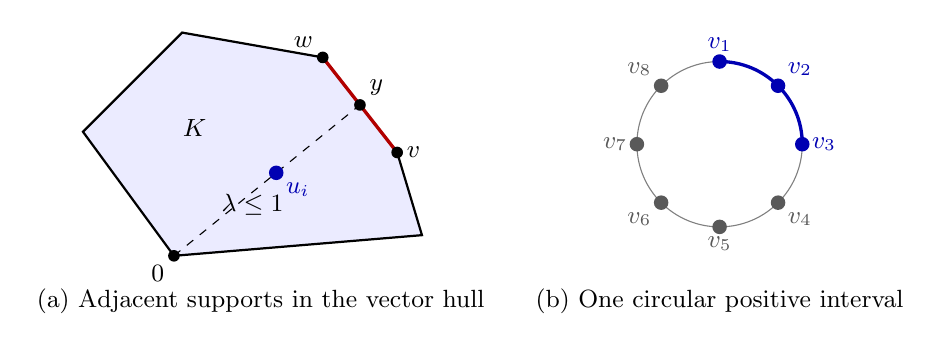
\begin{tikzpicture}[scale=1.05,every node/.style={font=\small}]
  % Query vectors and their adjacent hull supports.
  \fill[blue!8]
    (0,0)--(3,0.25)--(2.7,1.25)--(1.8,2.4)--(0.1,2.7)
    --(-1.1,1.5)--cycle;
  \draw[thick]
    (0,0)--(3,0.25)--(2.7,1.25)--(1.8,2.4)--(0.1,2.7)
    --(-1.1,1.5)--cycle;
  \draw[very thick,red!70!black] (2.7,1.25)--(1.8,2.4);
  \draw[dashed] (0,0)--(2.25,1.825);
  \fill (0,0) circle (2pt) node[below left] {$0$};
  \fill (2.7,1.25) circle (2pt) node[right] {$v$};
  \fill (1.8,2.4) circle (2pt) node[above left] {$w$};
  \fill (2.25,1.825) circle (2pt) node[above right] {$y$};
  \fill[blue!70!black] (1.2375,1.00375) circle (2.5pt)
    node[below right] {$u_i$};
  \node at (0.25,1.55) {$K$};
  \node at (0.95,0.62) {$\lambda\le1$};
  \node[align=center] at (1.05,-0.55)
    {(a) Adjacent supports in the vector hull};

  % A schematic cyclic order; blue vertices form one interval.
  \draw[gray] (6.6,1.35) circle (1);
  \draw[very thick,blue!70!black]
    (6.6,2.35) arc[start angle=90,end angle=0,radius=1];
  \fill[blue!70!black] (6.6,2.35) circle (2.5pt)
    node[above] {$v_1$};
  \fill[blue!70!black] (7.307,2.057) circle (2.5pt)
    node[above right] {$v_2$};
  \fill[blue!70!black] (7.6,1.35) circle (2.5pt)
    node[right] {$v_3$};
  \fill[gray!70!black] (7.307,0.643) circle (2.5pt)
    node[below right] {$v_4$};
  \fill[gray!70!black] (6.6,0.35) circle (2.5pt)
    node[below] {$v_5$};
  \fill[gray!70!black] (5.893,0.643) circle (2.5pt)
    node[below left] {$v_6$};
  \fill[gray!70!black] (5.6,1.35) circle (2.5pt)
    node[left] {$v_7$};
  \fill[gray!70!black] (5.893,2.057) circle (2.5pt)
    node[above left] {$v_8$};
  \node[align=center] at (6.6,-0.55)
    {(b) One circular positive interval};
\end{tikzpicture}
\caption{The first panel depicts normalized query vectors: $y$ lies
on the edge $vw$ and $u_i=\lambda y$ for
$0<\lambda\le1$. Writing $y=\theta v+(1-\theta)w$ gives
$u_i=\alpha v+\beta w$ with $\alpha+\beta=\lambda\le1$.
Consequently, if both support values on a hypothesis are at most
one, then $u_i\cdot x_h\le1$; equivalently,
$C_i\subseteq C_v\cup C_w$. The second panel shows the cyclic order
only; the positive hull tests of a fixed hypothesis form one
interval in that order.}
\label{fig:support-and-interval}
\end{figure}

\subsection{Interval hitting and discovery length}

A complete discovery route must hit every nonzero pattern. Once these
patterns are intervals, we can compute its smallest possible test set;
this will also provide the final budget in the batch construction.

\begin{lemma}[Minimum interval cover]\label{lem:minimum-interval-cover}
A minimum-cardinality hitting set for ordinary or circular intervals
on a finite candidate order is computable in polynomial time.
An empty demand is infeasible; an empty family needs no candidates.
\end{lemma}
\begin{proof}
On a line, an exchange argument permits choosing the right endpoint
of the earliest-ending demand. On a circle, enumerate one forced
hit and cut there; the remaining problem is linear. The detailed
exchange argument is given below.
\end{proof}

Priority and weight considerations can change the order in which tests
are chosen. We therefore also need a length bound for greedy discovery,
including the extra saving when the comparison cover has adjacent runs.
Here a demand is a nonempty interval of candidate positions, each demand
$I$ has a fixed weight $w(I)>0$, and a candidate's remaining weight is
the sum of $w(I)$ over currently unhit demands containing it. At each
step greedy chooses a candidate of maximum remaining weight; ties may
be resolved arbitrarily. The comparison cover $P$ is any finite set of
positions hitting every initial demand, $k=|P|$, and $c(P)$ counts its
maximal consecutive blocks in the full candidate order. After a greedy
choice, demands hit by that choice are deleted. The claimed bound holds
for every such cover $P$; taking a minimum cover gives the stated
special case.

\begin{lemma}[Greedy cover length with adjacent-run credit]
\label{lem:greedy-cover-length}
Let a nonempty family of positively weighted interval demands
be covered by a candidate set $P$ of size $k$. Let $c(P)$ be the
number of runs of consecutive candidates in $P$, measured in the
entire candidate order. Maximum-remaining-weight greedy finishes
within $k+c(P)-1$ choices, for every tie rule.
In particular, a minimum cover of size $k$ gives the usual bound
$2k-1$. For circular intervals the corresponding bound is $2k$.
\end{lemma}
\noindent
The extra term is the number of runs beyond the first. A scattered
cover may force greedy to spend choices repairing several gaps,
whereas a cover arranged in a few contiguous blocks has fewer such
gaps to repair.
\begin{proofstrategy}
Use the potential $|P|+c(P)$ for the still-active comparison cover.
An extreme choice can replace an extreme point of $P$ without changing
which positive-weight demands it hits. An interior choice partitions
the unhit demands into left and right interval families. The cover
parts on those sides have combined size plus run count at most the
previous potential. Induction pays for the first choice and then for
each nonempty side.
\end{proofstrategy}
\begin{proof}
Induct on the comparison cover size, separating extreme choices from
interior ones. Suppose first that the greedy choice $v$ lies left
of $P$, and let $u=\min P$. Every active interval containing $v$ also
contains $u$: it is covered by some $p\in P$, and the endpoint
inequalities give $v<u\le p$ inside that interval. Thus the hit-demand
set of $v$ is contained in the hit-demand set of $u$. Maximum remaining
weight gives $W(u)\le W(v)$, while containment and nonnegative weights
give $W(v)\le W(u)$. Since each weight is positive, the sets are equal,
so the two hit sets coincide. After querying $v$, every remaining
demand therefore avoids $u$ and is covered by some point of
$P'=P\setminus\{u\}$. The right extreme is symmetric. Since $u$ is an
extreme point, deleting it cannot split a run, so
$|P'|=k-1$ and $c(P')\le c(P)$. If demands remain, induction bounds
their greedy completion by
\[
 |P'|+c(P')-1\le k+c(P)-2.
\]
Including the current query gives at most $k+c(P)-1$ choices. If no
demand remains, the single current query already meets that bound.

Now suppose the greedy choice $v$ is interior. Every unhit interval lies wholly to one
side of $v$. Let $P_-$ and $P_+$ be the comparison points strictly to
its left and right. They cover the corresponding families. If $v\notin
P$, cutting the original order in its gap preserves the total number
of runs, so $c(P_-)+c(P_+)\le c(P)$ and their sizes sum to $k$.
If $v\in P$, the side sizes sum to $k-1$, and deleting $v$ can split
at most one run into two, so $c(P_-)+c(P_+)\le c(P)+1$. In either
case,
\[
 |P_-|+c(P_-)+|P_+|+c(P_+)\le k+c(P).
\]
The induction hypotheses bound the two side schedules by their
respective potentials minus one. Adding the current choice gives at
most $k+c(P)-1$. When only one side remains active, the unused side
has at least one comparison point and hence potential at least two;
this pays for the absent induction term. When neither side remains,
one choice is within the bound because $k\ge2$ in the interior case.
Finally $c(P)\le k$, since each run contains a distinct point of $P$;
therefore $k+c(P)-1\le2k-1$. For circular demands, the first greedy
choice cuts the circle and leaves ordinary intervals; the original
$k$ points still cover those intervals, giving at most $2k-1$ further
choices and the bound $2k$.
\end{proof}

\subsection{Recovering the interval endpoints}
\label{sec:endpoint-geometry}

A positive vertex locates a small cap. We recover the full pattern by
opening the circular order at a safe cut and comparing the interval's
endpoints against the supplied queries.

\begin{lemma}[Query-free endpoint representation]
\label{lem:legal-endpoint-queries}
After one positive hull vertex $v$ is known, a cut computable without
queries represents every compatible positive pattern as an ordinary
interval containing $v$. Supplied hull tests compare its endpoint
coordinates. A cached negative neighbor fixes one endpoint; two
negative neighbors fix the entire pattern.
\end{lemma}
\begin{proofstrategy}
Use a cached negative neighbor as the cut when available. Otherwise
the origin and an opposite hull edge give a cut that no compatible
positive interval can cross. All later comparisons are actual hull
tests, so no new line or anchor query is introduced.
\end{proofstrategy}
\begin{proof}
A cached negative neighbor supplies a cut and pins one endpoint.
Otherwise an opposite hull edge gives a cut without asking a query.
In the resulting linear order, supplied hull tests are endpoint
comparisons. Claims~\ref{clm:cached-endpoint},
\ref{clm:opposite-edge-cut}, and~\ref{clm:supplied-endpoint-comparisons}
establish these steps, including degenerate hulls.
\end{proof}

A positive discovery exit is \emph{pinned} if a neighbor of its
discovered vertex has a cached negative answer. It is
\emph{singly pinned} when exactly one neighbor is known negative,
and \emph{doubly pinned} when both are. Pinning fixes one or both
endpoints, as in Lemma~\ref{lem:legal-endpoint-queries}; it introduces no additional query.

\begin{algorithm}[H]
\caption{\EndpointCode: legal full-pattern recovery}
\label{alg:endpoint-code}
\KwIn{A positive hull vertex $v$, compatible patterns, cached answers;
code mode; optionally fixed continuation heights $h_A$.}
\KwOut{A supplied-query decoder whose leaves are full pattern classes.}
\If{the hull has dimension at most one}{\KwRet the already determined nonzero pattern\;}
\eIf{$v$ has a cached negative neighbor}{
  Cut at that neighbor and orient so $v$ is the first positive vertex\;
}{
  Cut at a boundary origin, or at the opposite edge met by the ray $v0$\;
}
List the realized left and right endpoint pairs in the cut order\;
\eIf{no continuation heights are supplied}{
  Search each unfixed endpoint using Algorithm~\ref{alg:alphabetic-code};
  condition the second search on the first answer\;
}{
  \ForEach{nonempty realized endpoint rectangle $U$, in increasing size}{
    \eIf{$U$ has a single realized class $A$}{$E(U)\gets h_A$\;}{
      $E(U)\gets\min_\ell(1+\max\{E(U\cap\ell^-),E(U\cap\ell^+)\})$,
      over proper supplied endpoint thresholds\;
    }
  }
  Reconstruct the minimizing rectangle splits, retaining full-pattern
  leaves and their recorded continuation heights\;
}
\KwRet the decoder; skip fixed endpoints and cached thresholds\;
\end{algorithm}

The cut turns the cyclic endpoint problem into a linear one, and
Lemma~\ref{lem:legal-endpoint-queries} shows that its thresholds are
supplied queries, so no extra anchor query is needed. If child heights
are provided, the rectangle recurrence compares each legal split by
the height of its endpoint subproblems together with the continuation
at the resulting pattern leaf. This is the complete-exit optimization
of Section~\ref{sec:polynomial-slots}. Its $O(M^4)$ rectangles and
$O(M)$ thresholds give polynomial running time. The routine returns
pattern leaves, after which the recursive algorithm attaches each
stored child once. The values $E(U)$ include the continuation heights
when comparing splits, while each child's query cost is accounted for
inside its attached recursive tree.



\subsection{Proofs of the geometric and interval facts}

The key step is to convert planar caps into executable endpoint
comparisons. Radial projection gives the one-way cover implication
needed by the analysis: every positive original cap is covered by its
support caps. The endpoint cut then follows from the geometry or from
cached answers, so it requires no additional query.

\begin{proof}[Proof of Lemma~\ref{lem:helly}]
There are two distinct tasks: obtain a common strict point from
flatness, then find such a point with controlled rational encoding.
The following claims separate the geometric existence argument from
its algorithmic realization.

\begin{claim}[Three majority half-planes have a common strict point]
\label{clm:majority-triples}
Every subfamily of at most three majority half-planes intersects.
\end{claim}
\begin{proof}
Use the measure defining flatness, either cardinality or probability.
By Definition~\ref{def:balanced}, each minority cap has measure
less than $\delta$ times the measure of $S$. The union bound
therefore makes the union of any three such caps have measure
less than $3\delta$ times that of $S$. Since $3\delta<1$,
that union omits a hypothesis.
That hypothesis belongs strictly to all three majority half-planes,
because no hypothesis lies on a query line. The same argument covers
subfamilies of fewer than three lines. Thus every subfamily of at
most three majority half-planes has nonempty intersection.
Theorem~\ref{thm:helly} implies
that the whole family has nonempty intersection.
\end{proof}

We now turn this strict intersection into the preprocessing algorithm's
witness. A positive-margin linear program finds a rational point with
polynomial encoding length, so the algorithm can compute and store it.

\begin{claim}[A positive margin gives a rational strict witness]
\label{clm:rational-witness}
The common point can be found with polynomial encoding length.
\end{claim}
\begin{proof}
To obtain a strict rational witness, orient each majority inequality
as $a_i\cdot p-b_i>0$ and maximize $t$ subject to
$a_i\cdot p-b_i\ge t$ for every $i$ and $0\le t\le1$.
The strict point obtained from Claim~\ref{clm:majority-triples}
and Theorem~\ref{thm:helly} has a positive value in each of the
finitely many inequalities. Their minimum, capped at one, supplies
a feasible positive $t$.
This is a \emph{linear program}: its objective and constraints
are linear in the unknown coordinates of $p$ and the margin $t$.
Rational linear programming therefore returns a strict witness
with polynomial encoding length~\cite{khachiyan1979}.
\end{proof}
\end{proof}

\begin{proof}[Proof of Lemma~\ref{lem:hull-structure}]
We establish the structure in three steps. First represent each query
by neighboring hull vertices; next prove the cap-cover implication;
finally identify the interval patterns and the unique possible
all-zero target. Each step is used by a different part of the algorithms.

\begin{claim}[Radial boundary projection needs only adjacent supports]
\label{clm:radial-supports}
Each normalized vector has a nonnegative support expression whose
coefficients sum to at most one.
\end{claim}
\begin{proof}
Extend the ray from $0$ through $u_i$ to its last point $y$ in $K$.
Such a point exists because the finite hull is compact and contains
$u_i\ne0$. Write $y=t u_i$ with $t\ge1$, so
$u_i=\lambda y$ for $\lambda=1/t\in(0,1]$.
If $y$ lies on an edge with endpoints $v,w$, write
$y=\theta v+(1-\theta)w$, with $0\le\theta\le1$. Then
\[
 u_i=(\lambda\theta)v+\lambda(1-\theta)w,\qquad
 \lambda\theta+\lambda(1-\theta)=\lambda\le1.
\]
The coefficients are nonnegative. Delete origin endpoints and zero coefficients
to obtain $J_i$. A boundary vertex needs only itself.
In dimension at most one, the last ray point is a segment endpoint,
so the same conclusion holds directly.
\end{proof}

The support expression is useful because it transfers a negative
answer from the hull tests back to the original query. Only this
one-way implication is needed to cover an optimal witness route.

\begin{claim}[Negative support answers force the original answer]
\label{clm:negative-supports}
The hull-cap inclusion \eqref{eq:hull-cap-cover} holds.
\end{claim}
\begin{proof}
If every support has $v\cdot x_h\le1$, the expression from
Claim~\ref{clm:radial-supports} gives
\[
 \begin{aligned}
 u_i\cdot x_h
 &=\sum_{v\in J_i}\alpha_{iv}(v\cdot x_h)\\
 &\le\sum_{v\in J_i}\alpha_{iv}\le1.
 \end{aligned}
\]
The first inequality uses the nonnegative support coefficients;
the second uses their sum bound. Thus a positive original query
must have a positive support, proving
\eqref{eq:hull-cap-cover}. Equality cannot occur at a hypothesis
because it would put it on the original supplied line.
The origin has dot product zero, so its bit is always negative
and it is never queried.
\end{proof}

Having justified cap coverage, we now describe the states produced
by hull tests. Their interval structure enables the scheduling tools;
the uniqueness of the zero pattern makes the final negative route valid.

\begin{claim}[The hull patterns are intervals with at most one zero point]
\label{clm:circular-patterns}
Every nonzero class belongs to a supplied positive hull cap.
\end{claim}
\begin{proof}
The positive vertices are $V\cap R_h$.
Here is why they are consecutive. Intersect the boundary line
$u\cdot x_h=1$ with the convex polygon $K$. Its intersection with
$K$ is empty or a segment; in a genuine crossing its two endpoints
cut the polygon boundary into two arcs, one on each side of the line.
The positive vertices lie on the positive arc. A tangency leaves
all vertices on one side and also gives an empty or consecutive block.
No hull query vertex lies on the boundary line, since that would
place $h$ on its supplied query. Removing the known-negative origin, if it is a vertex,
leaves a circular interval on $V$. Degenerate hulls have at most
two real vertices and satisfy the same assertion.
By Claim~\ref{clm:negative-supports}, an all-zero pattern forces
every original query to have the witness's answer. Two such
hypotheses would therefore have identical answers on all supplied
lines, contradicting separability.
Finally, a nonzero class has some positive vertex $v$, and all
its hypotheses belong to $C_v\cap S$.
\end{proof}
\end{proof}

\begin{proof}[Proof of Lemma~\ref{lem:minimum-interval-cover}]
For ordinary intervals, choose the right endpoint $q$ of an
earliest-ending interval $I$. Any cover has a point $u\in I$.
Replacing $u$ by $q$ loses no demand containing $u$: its right
endpoint is at least $q$, by the earliest-ending choice of $I$,
and its left endpoint is at most $u\le q$. Hence it also contains
$q$.
Thus an optimal cover can choose $q$. Delete the intervals hit
there and repeat, proving the endpoint greedy rule is exact.

For circular intervals, choose a nonempty demand and enumerate
a forced candidate $v$ in it. Delete demands hit by $v$ and cut
the cycle there. All remaining demands are ordinary intervals,
so use the preceding rule and add $v$. Some forced choice belongs
to an optimal circular cover; take the smallest resulting solution.
\end{proof}

\begin{proof}[Proof of Lemma~\ref{lem:greedy-cover-length}]
Induct on $k$. When $k=1$, its sole candidate hits every demand,
and any greedy maximum does so as well.
Let $v$ be the first greedy choice.

At an extreme, greedy removes the same demands as one comparison-cover
point. We can therefore delete that point from the comparison cover,
which gives the induction step that reduces the cover size.

\begin{claim}[An extreme greedy choice removes an extreme cover point]
\label{clm:greedy-extreme}
The remaining demands admit the cover $P\setminus\{u\}$ with no
increase in run count.
\end{claim}
\begin{proof}
If $v$ lies at or outside an
extreme of $P$, let $u$ be the nearest extreme cover point.
For example, if $v<\min P=u$, every demand containing $v$ must also
meet $P$, and hence must contain $u$: if $p\in P$ is a point of that
demand, then $v<u\le p$ and the demand is an interval. Thus the demands
hit by $v$ are a subset of those hit by $u$, which gives
$W(v)\le W(u)$ by summing nonnegative weights. Greedy maximality gives
$W(u)\le W(v)$, so the scores are equal. Because every weight is
strictly positive, a proper containment would make the second score
strictly larger; hence the candidates hit the same demands.
Thus $P\setminus\{u\}$ covers the remainder, and removing an
extreme leaves its run count unchanged or smaller. Induction plus the first
query gives at most $k+c(P)-1$ choices.
\end{proof}

For an interior choice, the comparison cover may retain all its points.
The unhit demands then split into independent left and right
subproblems, whose combined size-plus-run charge supplies the required
progress.

\begin{claim}[An interior choice creates independent left and right problems]
\label{clm:greedy-interior}
The sum of their size-plus-run charges is at most $k+c(P)$.
\end{claim}
\begin{proof}
Otherwise $v$ lies strictly between the extremes of $P$.
The unhit intervals lie entirely on one side of $v$.
The parts $P_-,P_+$ strictly to its left and right cover these
two families, and
\[
 |P_-|+c(P_-)+|P_+|+c(P_+)\le k+c(P).
\]
If $v\notin P$, cutting in its gap leaves the total run count
unchanged. If $v\in P$, removing it reduces size by one and can
increase total run count by at most one, which proves the displayed
inequality in either case. Runs are measured against the full candidate
order, so truncating to the two sides creates no new gap boundary except
at the removed $v$. Greedy may interleave the two sides, but
a choice on one side covers no interval on the other; hence the
choices restricted to either side are still a greedy sequence for
that side. If both families are nonempty, each side has a smaller
comparison cover than $P$. Applying the induction hypothesis to
both sides and paying for the first query gives
\[
 1+\bigl(|P_-|+c(P_-)-1\bigr)
   +\bigl(|P_+|+c(P_+)-1\bigr)\le k+c(P)-1.
\]
The last inequality substitutes the preceding bound on their
combined size-plus-run charge.
If only one is nonempty, the other cover part still has size plus
run count at least two. If $P_{\rm live}$ covers the nonempty side,
the total is at most
\[
 1+\bigl(|P_{\rm live}|+c(P_{\rm live})-1\bigr)
 \le k+c(P)-2\le k+c(P)-1.
\]
Here induction bounds the live side, while the unused side's
charge of at least two bounds its complement in $k+c(P)$: at least one
point remains on that side since $v$ lies strictly between the extremes,
and one nonempty run contributes one to each term.
If neither remains, one query suffices, and $k\ge2$ in this interior
case ensures $1\le k+c(P)-1$.
\end{proof}
Claims~\ref{clm:greedy-extreme} and~\ref{clm:greedy-interior}
complete the induction. Finally $c(P)\le k$, because each run
contains a distinct cover point, giving $2k-1$ without adjacency
information.

For circular intervals, make the first greedy choice and cut the
cycle there. Every unhit interval becomes an ordinary interval.
The original $k$ cover candidates still cover these demands,
so at most $2k-1$ further choices are needed.
\end{proof}

\begin{proof}[Proof of Lemma~\ref{lem:legal-endpoint-queries}]
First exploit a cached negative answer if one exists. Otherwise find a
safe cut geometrically. After either construction, verify that the
resulting endpoint searches ask only supplied hull queries.

\begin{claim}[A cached negative neighbor pins an endpoint]
\label{clm:cached-endpoint}
Only the opposite endpoint remains to be learned.
\end{claim}
\begin{proof}
After discovery, one positive hull vertex $v$ is known.
First inspect its cached neighbor answers. If a neighbor is known
to be negative, cut at that vertex and orient the order so that
$v$ is first. The positive interval starts at $v$, so only its
other endpoint needs a search. If both neighbors are negative,
the pattern consists of $v$ alone and no endpoint query is needed.
\end{proof}

When the discovery path has no cached negative neighbor, the geometry
supplies the cut. The origin's known-negative position ensures that a
compatible positive interval cannot cross the opposite edge.

\begin{claim}[The opposite-edge cut costs no query]
\label{clm:opposite-edge-cut}
Without a cached cut, the normalized hull supplies a cut that no
compatible positive interval can wrap around.
\end{claim}
\begin{proof}
Otherwise use a geometric cut. If the origin lies on the hull
boundary, cut at its free negative
marker. If it is interior, the ray from $v$ through $0$ meets
an opposite hull edge with consecutive endpoints $a,b$.
The origin is a convex combination of $v,a,b$, with positive
coefficient on $v$. Explicitly, the intersection point is
$y=-tv$ for some $t>0$ and $y=\theta a+(1-\theta)b$, so
\[
 0=\frac{t}{1+t}v+\frac{\theta}{1+t}a
                       +\frac{1-\theta}{1+t}b.
\]
The coefficients are nonnegative and sum to one. If $a,b$ were
both positive, then $v\cdot x_h,a\cdot x_h,b\cdot x_h>1$, giving
\[
 \begin{aligned}
 0=0\cdot x_h
 &=\frac{t}{1+t}(v\cdot x_h)
   +\frac{\theta}{1+t}(a\cdot x_h)
   +\frac{1-\theta}{1+t}(b\cdot x_h)\\
 &>\frac{t+\theta+(1-\theta)}{1+t}=1,
 \end{aligned}
\]
a contradiction. The strict step multiplies the positive test
values by nonnegative coefficients; the coefficient of $v$ is
strictly positive, so the sum is strictly greater than one even
if an opposite-edge coefficient vanishes.
Cut the cyclic order between $a$ and $b$. A circular positive
interval could wrap around this cut only if both endpoints
were positive, which was just excluded. If the ray meets a
vertex $y$, then $y\cdot x_h=-t(v\cdot x_h)<0<1$ for every
compatible hypothesis, so it is a free negative cut point.
\end{proof}

The cut has removed wrap-around. We can now verify that learning the
two endpoints amounts to asking existing hull tests, which is essential
for keeping the construction within the supplied-query model.

\begin{claim}[Endpoint comparisons are supplied hull queries]
\label{clm:supplied-endpoint-comparisons}
Both endpoint searches, including their degenerate cases, are legal.
\end{claim}
\begin{proof}
By Claims~\ref{clm:cached-endpoint} and~\ref{clm:opposite-edge-cut},
the positive vertices now form an ordinary interval containing
$v$, obtained without an anchor query. To its left, querying a vertex asks whether
the left endpoint is at or before that vertex. To its right,
querying a vertex asks whether the right endpoint is at or after it.
Thus supplied hull queries give the ordered comparisons needed to
locate the two endpoints.



When neither endpoint is already fixed, learn the left endpoint,
then the right endpoint conditioned on
the left endpoint and the earlier transcript. For consecutive
possible left endpoints, querying the earlier endpoint separates
them; for consecutive possible right endpoints, querying the later
endpoint separates them. These are real hull vertices, so all
comparisons used by the alphabetic codes of
Lemma~\ref{lem:alphabetic-endpoints} are supplied queries.
The conditional endpoint distributions come from the hypothesis table.

If $K$ has dimension at most one, it has at most two real vertices.
With two real endpoints, one positive endpoint forces the other
negative because $0$ lies between them. With one real vertex,
its positive bit is the complete nonzero pattern.
Thus no further query is needed in either degenerate case.
\end{proof}
\end{proof}

\section{Maximum-depth scheduling ingredients}
\label{sec:worst}

The maximum-depth algorithm of Section~\ref{sec:polynomial-slots}
constructs its pattern children first and then schedules their discovery.
This section isolates its local tools. The priority scheduler extends
the construction beyond the exact scheduler's logarithmic rank cap by
supplying a passing height trial. All branch decisions use hypothesis
counts and supplied-line geometry.

Let $\delta\in(0,1/3)$ be the count-balance threshold and let $\gamma>2$
be the coefficient of the count potential
$\Phi(s)=\lfloor\gamma\log_2s\rfloor$. Assume
\begin{equation}\label{eq:worst-parameter-conditions}
 \gamma\log_2\frac1{1-\delta}\ge1,\qquad
 \gamma\log_2\frac1\delta\ge5.
\end{equation}
The first inequality pays for a balanced query; the second pays for
endpoint recovery at a flat state. Section~\ref{sec:worst-calibration}
chooses the constants at the point where these two credits balance.

For a state $S$, write $C_W(S)$ for the height of the tree returned
by the hybrid recursive algorithm. When a proof refers to a stored
child code, its height is the actual height of that code.

\subsection{Local credits and the priority fallback}

\begin{proofstrategy}
\begin{enumerate}
\item Restrict an optimal tree to a pattern class: its common witness
prefix disappears and gives that class a discovery deadline.
\item Recover the pattern with supplied endpoint comparisons; the
count-potential drop pays for this decoder.
\item Use priorities to meet all deadline prefixes in one ordering.
Every accepted ordering is checked against actual stored child heights.
\end{enumerate}
\end{proofstrategy}

In a count-flat state $S$ of size $s$, use the common witness and hull
patterns of Lemmas~\ref{lem:helly} and~\ref{lem:hull-structure}.
Every nonzero class $A$ has $a=|A|<\delta s$; the zero class $A_0$
is empty or a singleton. Write
\[
 z_A=\lfloor\log_2(\delta s/a)\rfloor.
\]
All child heights below come from already constructed codes; the
optimal tree appears only in the comparison argument.

The recursion needs integer query allowances, while its potential uses
logarithms. The following credit converts size reduction into a whole
query at a balanced split and enough whole queries for a flat decoder.

\begin{proposition}[Integer count credit]\label{lem:worst-floor-credit}
A balanced child of size $a\le(1-\delta)s$ satisfies
$\Phi(s)-\Phi(a)\ge1$. A nonzero flat-state class satisfies
\begin{equation}\label{eq:worst-floor-credit}
 \Phi(s)-\Phi(a)\ge\lfloor\gamma\log_2(s/a)\rfloor\ge z_A+5.
\end{equation}
\end{proposition}

For a flat state, the optimal tree supplies an analytical comparison
schedule. Its initial witness answers are constant on a class until
that class meets a support; restriction turns this delay into saved
height inside the class.

\begin{proposition}[Supporting-prefix credit]\label{lem:height-prefix}
Follow a common witness in a proper optimal tree of height
$D=\OPT_W(S)$ along a path of length $r$. Let $t_A$ be the first
path query whose real hull supports meet the positive pattern of $A$;
put $t_A=r+1$ if none does. Then
\[
 \OPT_W(A)\le D-(t_A-1).
\]
The supporting singleton or adjacent-pair blocks cover every nonzero
class by its index $t_A$, after appending one positive support for an
uncovered terminal nonzero singleton when necessary.
\end{proposition}

A first positive answer locates one vertex of the pattern. The endpoint
decoder then recovers the full interval, with a pointwise cost bound so
maximum depth controls each class separately.

\begin{proposition}[Legal endpoint allowances]\label{lem:endpoint-height}
After a first positive hull answer, the pointwise alphabetic endpoint
codes recover class $A$ with at most
\[
 e_A^{(4)}=z_A+4
\]
additional supplied queries. If a neighboring hull vertex is already
known negative, one endpoint is fixed and the allowance is
$e_A^{(2)}=z_A+2$. A hull of dimension at most one needs no further
query after discovery.
\end{proposition}

Scheduling can now use the codes already built for the children.
Adding their actual heights to discovery and endpoint recovery gives
a directly checkable route certificate, including the all-negative route.

\begin{proposition}[Local route-height certificate]\label{lem:worst-local-height}
Let $h_A$ be a stored class code's actual height. Discover a positive
vertex in a fixed ordering truncated when all nonzero patterns are
covered. If its first positive position for $A$ is $g_A$, the whole
route through $A$ has height at most $g_A+h_A+e_A^{(4)}$, or
$g_A+h_A+e_A^{(2)}$ on a pinned exit. If every such bound is at most
$H$, the whole tree has height at most $H$, including its zero route
when that class exists.
\end{proposition}

The classes have different deadlines, yet the algorithm must choose
one query order. Integer priorities make later deadlines unable to
interfere with greedy progress on any earlier deadline prefix.

\begin{proposition}[One ordering for all block deadlines]
\label{lem:deadline-cover}
Force an oriented adjacent real pair $(v,w)$ first. Consider only
classes negative on both, with integer block deadlines $d_A\ge2$.
Suppose a comparison sequence begins with $\{v,w\}$ and hits $A$
within $d_A$ singleton or adjacent-pair blocks. Sort the distinct
budgets as $d^{(1)}<\cdots<d^{(r)}$, give a deadline-$d^{(j)}$ class
weight $(s+1)^{r-j}$, and complete by maximum-remaining-weight greedy.
This polynomial-time ordering satisfies $g_A\le3d_A-2$
for every surviving class simultaneously.
\end{proposition}

The endpoint and prefix credits turn the optimal witness path into
deadlines, and the priority ordering meets those deadlines. It therefore
provides a passing trial even when the capped exact scheduler cannot
certify the stronger bound.

\begin{proposition}[Priority fallback height]
\label{thm:worst}
Suppose stored pattern children satisfy the fallback bound
\[
h_A\le3\OPT_W(A)+\Phi(|A|).
\]
At a flat state,
Algorithm~\ref{alg:priority-trial} has a passing trial at
\[
 H^*=3\OPT_W(S)+\Phi(s).
\]
A balanced query also fits this height if its two stored children
obey the same bound. Consequently the hybrid recursion can always
retain $C_W(S)\le3\OPT_W(S)+\Phi(s)$ as its fallback invariant.
\end{proposition}

For a trial $H$ and a forced pair, first-positive exits must pass
$1+h_A+e_A^{(4)}\le H$, and second-query exits must pass
$2+h_A+e_A^{(2)}\le H$. Classes negative on both receive
\[
 u_A=h_A+e_A^{(4)},\qquad B_A=H-u_A,\qquad
 d_A=\lfloor(B_A+2)/3\rfloor.
\]
Reject any $B_A<4$ and accept only after checking the resulting
actual first-hit positions against $g_A+u_A\le H$.
These tests describe an executable height certificate; the optimal
comparison blocks are used only to prove that some trial passes.

For a fixed target height $H$, each oriented adjacent pair determines
which patterns are hit at its first endpoint, second endpoint, or
neither. The first two groups have immediate local height tests, so a
pair that already exceeds $H$ can be discarded. For patterns left on
the miss route, the remaining height becomes a deadline; the priority
weights make the greedy order favor the tightest deadlines. The final
check uses the actual hit ranks and child allowances, and accepts the
order only when every miss-route pattern fits.

\begin{algorithm}[H]
\caption{\PriorityTrial: internal fallback for one height trial}
\label{alg:priority-trial}
\KwIn{Flat state's hull and classes; child heights $h_A$; allowances $e_A^{(4)},e_A^{(2)}$; target $H$.}
\KwOut{A passing discovery order, or infeasible.}
\ForEach{oriented adjacent real pair $(v,w)$}{
  Form $\mathcal F,\mathcal S,\mathcal N$ by their first hit on $(v,w)$\;
  \If{some $A\in\mathcal F$ has $1+h_A+e_A^{(4)}>H$, or
  some $A\in\mathcal S$ has $2+h_A+e_A^{(2)}>H$}{\Continue\;}
  \ForEach{$A\in\mathcal N$}{
    $u_A\gets h_A+e_A^{(4)}$;
    $B_A\gets H-u_A$;
    $d_A\gets\lfloor(B_A+2)/3\rfloor$\;
  }
  \If{some $B_A<4$}{\Continue\;}
  Sort distinct budgets as $d^{(1)}<\cdots<d^{(r)}$\;
  Give each deadline-$d^{(j)}$ class weight $(|S|+1)^{r-j}$\;
  Force $v,w$ and complete by maximum-remaining-weight greedy;
  truncate when all nonzero classes are hit\;
  \If{every $A\in\mathcal N$ has actual $g_A+u_A\le H$}{\KwRet this order\;}
}
\KwRet infeasible\;
\end{algorithm}


\subsection{Technical proofs of the local ingredients}

\begin{proof}[Proof of Proposition~\ref{lem:worst-floor-credit}]
For real $x,y$, write $x-y=k+\theta$ with integer
$k=\lfloor x-y\rfloor$ and $0\le\theta<1$. Then
$\lfloor x\rfloor=\lfloor y+k+\theta\rfloor
\ge\lfloor y\rfloor+k$, proving the floor-difference inequality.
Apply it to the two count potentials:
\[
 \Phi(s)-\Phi(a)
 \ge\left\lfloor\gamma\log_2(s/a)\right\rfloor.
\]
Indeed, the difference of the unfloored logarithms is
$\gamma\log_2s-\gamma\log_2a=\gamma\log_2(s/a)$, which is the
argument to the floor-difference inequality. For a balanced child,
$a\le(1-\delta)s$, hence $s/a\ge1/(1-\delta)$. The first
condition in \eqref{eq:worst-parameter-conditions} therefore gives
\[
 \gamma\log_2(s/a)
 \ge\gamma\log_2\frac1{1-\delta}\ge1.
\]
Since every real number at least one has floor at least one, the
balanced-child claim follows, including the equality case.
For a flat class put $x=\log_2(s/a)$ and
 $\ell=\log_2(1/\delta)$. Since $a<\delta s$, we have $x>\ell$.
The calibration gives $\gamma\ell=5$, so, using $\gamma>1$,
\[
 \gamma x=\gamma\ell+\gamma(x-\ell)
          =5+\gamma(x-\ell)>5+(x-\ell).
\]
Monotonicity of the floor therefore gives
\[
 \left\lfloor\gamma x\right\rfloor
 \ge\lfloor5+x-\ell\rfloor
 =5+\lfloor\log_2(\delta s/a)\rfloor=5+z_A,
\]
which proves the flat credit including its integer rounding.
\end{proof}

\begin{proof}[Proof of Proposition~\ref{lem:height-prefix}]
There are two distinct steps. Common answers give a restriction credit;
supporting blocks then cover the positive classes with deadlines measured
from the same witness path. The terminal leaf needs separate attention
because the witness may end at a real hypothesis with a nonzero pattern.
Claims~\ref{clm:height-prefix-constant} and
\ref{clm:height-comparison-cover} establish these two steps, respectively.

\begin{claim}[The common prefix disappears under restriction]
\label{clm:height-prefix-constant}
Every member of $A$ follows the witness's first $t_A-1$ answers.
\end{claim}
\begin{proof}
For every index $i<t_A$, no support of the $i$th query meets the positive
pattern of $A$. Lemma~\ref{lem:hull-structure} then makes its answer
constant on $A$, with the same value as on the witness. This includes a
query whose support uses the free origin marker. Thus every member of $A$
traverses the same first $t_A-1$ nodes of the optimal tree.

Restrict that tree to $A$. Since $A$ is nonempty and each of those answers
is constant, each corresponding node contracts to its witness-side child.
The remaining tree identifies $A$ and has height at most
$D-(t_A-1)$: each original path had length at most $D$, and the shared
prefix has been removed from every such path. Minimizing over identifying
trees on $A$ proves the inequality.

\end{proof}
The restriction credit must come with a cover that can be compared
against a scheduler. Queries along the path cover every class except,
possibly, the hypothesis at its terminal leaf.

\begin{claim}[The supporting blocks form a comparison cover]
\label{clm:height-comparison-cover}
Only an uncovered terminal nonzero singleton needs an appended block.
\end{claim}
\begin{proof}
Each class with $t_A\le r$ is hit by that path query's supports.
By Claim~\ref{clm:height-prefix-constant}, an unhit class follows
the entire original path and is therefore the
single leaf hypothesis reached by the witness. If its pattern is
nonzero, append a positive hull vertex at index $r+1$; if it is zero,
the witness leaf already completes the cover. Retaining the first
occurrence of a repeated support preserves every first-hit deadline.
\end{proof}
\end{proof}

\begin{proof}[Proof of Proposition~\ref{lem:endpoint-height}]
The query-free cut of Lemma~\ref{lem:legal-endpoint-queries} makes the
positive pattern an ordinary interval. Let $R$ be the hypotheses
compatible with the first positive transcript, so $|R|<\delta s$.
Use uniform counts, conditioned on that transcript, as code-design
probabilities, while the algorithm itself follows the deterministic
construction.
The two conditional endpoint probabilities multiply to the probability
of the full class. Their logarithmic query bounds therefore telescope
to one bound depending on the class size.
Claims~\ref{clm:height-two-endpoints} and~\ref{clm:height-pinned-endpoint}
establish the two allowances, according to whether discovery has
already fixed a boundary.

\begin{claim}[Two endpoint searches telescope their probabilities]
\label{clm:height-two-endpoints}
If $a_L$ compatible hypotheses have the target's left endpoint, its
full pattern is learned in fewer than $\log_2(\delta s/a)+4$ queries.
\end{claim}
\begin{proof}
Lemma~\ref{lem:legal-endpoint-queries} makes both searches legal.
Applying the pointwise bound of Lemma~\ref{lem:alphabetic-endpoints}
to the first endpoint and then to the conditional second endpoint gives
\[
 \log_2\frac{|R|}{a_L}+2+
 \log_2\frac{a_L}{a}+2
 =\log_2\frac{|R|}{a}+4<\log_2\frac{\delta s}{a}+4.
\]
The logarithms add because
$(|R|/a_L)(a_L/a)=|R|/a$: the second distribution is conditioned
on the learned first endpoint. The endpoint pair uniquely specifies
the pattern, while the strict inequality uses $|R|<\delta s$:
the first positive transcript confines $R$ to one minority cap.
If $q_A$ is the integer number of endpoint queries,
the displayed strict bound gives
$q_A<\log_2(\delta s/a)+4<z_A+5$. Thus
$q_A\le z_A+4$, including when the logarithm itself is an integer.
\end{proof}
A negative neighbor supplies more information than ordinary discovery:
it fixes an endpoint. This removes an entire endpoint search and gives
the extra saving needed on the second exit of the initial pair.

\begin{claim}[A cached negative neighbor removes one search]
\label{clm:height-pinned-endpoint}
A pinned positive vertex fixes one interval endpoint.
\end{claim}
\begin{proof}
Cut at the negative neighbor and orient the order to place the
positive vertex first. Lemma~\ref{lem:legal-endpoint-queries}
fixes that boundary; hence Lemma~\ref{lem:alphabetic-endpoints}
requires only one search to learn the other endpoint
in fewer than $\log_2(\delta s/a)+2$ queries. Writing its integer
query count as $q_A$, we have
$q_A<\log_2(\delta s/a)+2<z_A+3$, hence $q_A\le z_A+2$.
The negative neighbor is a real cached answer, so no anchor
query is added. In dimension at most one the positive pattern is
already determined; inference and cached answers can only lower cost.
\end{proof}
\end{proof}

\begin{proof}[Proof of Proposition~\ref{lem:worst-local-height}]
A route through $A$ makes at most $g_A$ discovery queries,
then uses the endpoint allowance of Proposition~\ref{lem:endpoint-height},
and finally follows a stored
code of height $h_A$. Its height is their sum, bounded by $H$ by
hypothesis. The ordering is truncated as soon as all nonzero classes
are covered, namely after at most $\max_{A\ne A_0}g_A$ queries.
Since $h_A$ and both endpoint allowances are nonnegative, the route
tests imply $g_A\le H$ for each nonzero class. Thus the all-negative
route also has length at most $H$ and ends at the zero singleton. If that class is absent its leaf is
omitted. A nonsingleton state has a nonzero pattern because
Lemma~\ref{lem:hull-structure} gives $|A_0|\le1$.
\end{proof}

\begin{proof}[Proof of Proposition~\ref{lem:deadline-cover}]
The proof separates priorities from geometry. First, the priorities
make the global order greedy for every nested deadline prefix. Then
an interval-cover bound limits the number of queries for each prefix.

\begin{claim}[Later deadlines cannot change a prefix greedy choice]
\label{clm:deadline-priority-prefix}
The global ordering is weighted greedy for every surviving deadline
prefix until that prefix is covered.
\end{claim}
\begin{proof}
Put $U=(s+1)^{r-j}$. A class of earlier or equal deadline has
weight $U(s+1)^{j-i}$ for some $i\le j$, so every candidate's
prefix score is an integer multiple of $U$. For $j<r$, all later
classes together have weight at most
\[
 s(s+1)^{r-j-1}=\frac{s}{s+1}U<U;
\]
for $j=r$ their total is zero. Deleting already hit classes can only
lower these totals. If one candidate's prefix score exceeds another's,
it exceeds it by at least $U$; no difference in their later-class
scores can reverse that comparison. Therefore a global score maximizer
also maximizes the prefix score. A nonzero prefix score is at least
$U$ and beats every zero prefix score while demands remain. Global
tie-breaking chooses among legitimate prefix greedy ties.
This applies to every deadline prefix at every step of the same order.
\end{proof}
The prefix argument determines which demands each greedy choice serves.
To bound the number of choices, use the forced adjacent pair to cut the
line of blocks and remove its first block; the remaining cover's size
and runs then pay for every later greedy choice.

\begin{claim}[The first pair leaves at most $3d-4$ later greedy choices]
\label{clm:deadline-prefix-length}
A nonempty deadline-$d$ prefix finishes by actual position $3d-2$.
\end{claim}
\begin{proof}
Cut at $v$ and delete its adjacent vertex $w$. Surviving demands are
ordinary intervals. Remove these two vertices from the union $P$
of the first $d$ comparison blocks. Each of the other $d-1$ blocks
contributes at most three to $|P|+c(P)$, where $c(P)$ counts runs:
a pair contributes at most two vertices and one run, and a singleton
at most one vertex and one run. Deleting the two adjacent cut vertices
cannot split any surviving adjacent-pair block. For finite sets
$U,V$ on a line, $|U\cup V|\le|U|+|V|$ and
$c(U\cup V)\le c(U)+c(V)$: joining runs cannot create a new run.
Applying these inequalities to the remaining $d-1$ blocks gives
$|P|+c(P)\le3(d-1)$. Every prefix demand misses the forced pair
and was hit by one of these remaining blocks, so $P$ still covers it.
By Claim~\ref{clm:deadline-priority-prefix}, the actual later
choices form a greedy sequence for this prefix. Consequently
Lemma~\ref{lem:greedy-cover-length} bounds their number by
\[
 |P|+c(P)-1\le3(d-1)-1=3d-4.
\]
The inequality uses the size-plus-run bound just established;
the equality simplifies the resulting integer allowance.
Adding the two forced queries gives position at most $3d-2$. An empty prefix needs no further choice.
\end{proof}
The auxiliary weights have $O(s\log s)$ bits, and their incidence
scores are computed from the explicit class-to-vertex table. Thus the
ordering and actual first-hit times have polynomial bit complexity.
\end{proof}

\begin{proof}[Proof of Proposition~\ref{thm:worst}]
Put $D=\OPT_W(S)$. For a balanced child $A$, restriction and
count credit, specifically Lemma~\ref{lem:restriction} and
Proposition~\ref{lem:worst-floor-credit}, give
\[
 \OPT_W(A)\le D,\qquad \Phi(|A|)\le\Phi(s)-1.
\]
Thus its complete route satisfies
\[
 1+h_A\le1+3\OPT_W(A)+\Phi(|A|)
          \le3D+\Phi(s)=H^*.
\]
The first inequality is the stored-child invariant. The second
substitutes the two preceding bounds, so the potential drop pays
for the new root query.
At a flat state,
enumerate an initial pair containing the first optimal-witness query's
supports; pad a singleton support by an adjacent real neighbor.
The first two exits must be checked directly: the deadline scheduler
handles only classes that miss both initial queries. The cached
negative answer makes the second positive exit cheaper to decode.

\begin{claim}[Both initial positive exits fit $H^*$]
\label{clm:fallback-initial-exits}
The first-query exit has at least one query of discovery credit;
the pinned second-query exit has at least three.
\end{claim}
\begin{proof}
For either class, Lemma~\ref{lem:restriction} gives
$\OPT_W(A)\le D$. Using the stored-child invariant and then
Proposition~\ref{lem:worst-floor-credit},
\[
 H^*-h_A\ge3D+\Phi(s)
                -3\OPT_W(A)-\Phi(|A|)
             \ge\Phi(s)-\Phi(|A|)
             \byref{Prop.}{lem:worst-floor-credit}{\ge}z_A+5.
\]
The middle inequality drops the nonnegative difference
$3(D-\OPT_W(A))$. Thus the first positive exit satisfies
$1+h_A+(z_A+4)\le H^*$. By Proposition~\ref{lem:endpoint-height},
the second positive exit has a cached negative neighbor and only
the smaller allowance, so
$2+h_A+(z_A+2)\le H^*-1\le H^*$.
Neither calculation assumes that the class meets the original support;
restriction and flat count credit also cover classes hit only by
the padding vertex.
\end{proof}
For the remaining classes, the supporting-prefix credit becomes an
integer block deadline. The floor below preserves that credit exactly,
so the comparison schedule meets the deadlines computed from actual
child heights.

\begin{claim}[Every later class meets its computed deadline]
\label{clm:fallback-later-deadline}
For a class negative on the initial pair, $d_A\ge t_A$.
\end{claim}
\begin{proof}
Here $t_A\ge2$, because this class misses the first query's
supports. Proposition~\ref{lem:height-prefix} and the actual
child invariant give
$h_A\le3[D-(t_A-1)]+\Phi(|A|)$. Substituting this into the
budget and then using count credit yields
\begin{align*}
 B_A&=3D+\Phi(s)-h_A-(z_A+4)\\
    &\ge3(t_A-1)+\Phi(s)-\Phi(|A|)-(z_A+4)\\
    &\byref{Prop.}{lem:worst-floor-credit}{\ge}3(t_A-1)+(z_A+5)-(z_A+4)
      =3t_A-2\ge4.
\end{align*}
Hence $(B_A+2)/3\ge t_A$; since $t_A$ is an integer,
$d_A=\lfloor(B_A+2)/3\rfloor\ge t_A$.
The padded first block and the remaining comparison blocks, including
the terminal singleton block if needed, satisfy
Proposition~\ref{lem:deadline-cover}. Its ordering has
\[
 g_A\le3d_A-2=3\lfloor(B_A+2)/3\rfloor-2\le B_A.
\]
The first inequality is Proposition~\ref{lem:deadline-cover};
the equality substitutes the computed deadline.
To justify the last inequality, write $B_A+2=3d_A+r_A$ with
$r_A\in\{0,1,2\}$. Then $3d_A-2=B_A-r_A\le B_A$,
so adding $u_A=h_A+e_A^{(4)}$ gives $g_A+u_A\le H^*$.
\end{proof}
The deadline argument bounds every route that uses block scheduling,
including the truncated zero route, by
Proposition~\ref{lem:worst-local-height} and
Claims~\ref{clm:fallback-initial-exits}--\ref{clm:fallback-later-deadline}.
When the hull has dimension at most one, the scheduler is unnecessary:
Lemma~\ref{lem:legal-endpoint-queries} shows that two extreme tests
determine the pattern and leave no endpoints to decode. A nonzero class
then costs at most $2+h_A$. The stored-child, restriction, and
count-credit calculation from Claim~\ref{clm:fallback-initial-exits}
gives
\[
 2+h_A\le3D+\Phi(s)-z_A-3\le H^*.
\]
The second inequality uses $z_A\ge0$ and the definition of $H^*$.
The zero route also ends after at most the two extreme tests. Thus the
local fallback bound holds in every dimension, and induction gives the
stated invariant for the hybrid tree.
\end{proof}

\section{Scheduling the first positive answer}
\label{sec:scheduling}

The maximum-depth algorithm must coordinate discovery with the heights
of its child codes. Expected depth poses a different scheduling need:
caps containing likely targets should be tested early, which leads to
weighted min-sum set cover (MSSC). We use the supplied caps as the
covering sets, with a singleton cap included whenever a supplied test
realizes it.

In the decision-tree application, a positive hull answer exits the
all-negative route and reveals that the target lies in a small cap.
The all-zero pattern follows that route through every test; once the
schedule has covered every positive pattern, the all-zero class is the
remaining outcome. An earlier singleton inference shortens its route.
Its expected-cost contribution is therefore bounded by its weight
times the schedule length. Accordingly, our ordering bound tracks both
the sum of positive-pattern first-cover times and the length paid on
the all-negative route.

\begin{symboltable}
$U,\ \pi_h,\ p_0$ & Coverable positive-pattern demands, their positive weights, and the weight of a target found only after the schedule finishes.\\
$t_Q(h),\ \MSSC(Q)$ & First-cover position of demand $h$ in ordering $Q$ and the sum $\sum_h\pi_h t_Q(h)$.\\
$k_0$ & Minimum number of candidate tests needed to cover all demands in $U$.\\
$\beta,\ \Phi_\beta,\ Z_\beta$ & Geometric budget factor and the first-cover and total-length accounting functions.\\
$r_Q(x),\ G_u$ & Comparison-order mass with first-cover time greater than $x$, and the constructed schedule for shift $u$.\\
\end{symboltable}

Weighted MSSC has a classical greedy four-approximation~\cite{flt2004}.
For circular intervals, we obtain a stronger guarantee by first solving
the maximum-coverage problem exactly for each cardinality budget.
Ordering these budget-optimal sets in geometric batches then controls
both first-cover cost and total length.

This batch method extends minimum cover by optimizing covered weight
at every integer budget. The interval structure makes each optimization
tractable: once the previous selected position is known, the next
position determines the newly covered demands.

\begin{lemma}[Exact budgeted interval coverage]\label{lem:budget-coverage}
For positively weighted interval or circular-interval demands on
a finite candidate set, a set of at most $k$ candidates hitting
maximum demand weight is computable in polynomial time.
\end{lemma}
\begin{proof}
Algorithm~\ref{alg:interval-cover} gives both interval oracles.
For ordinary intervals, number the candidates $1,\ldots,M$.
If the previous selected candidate is $p$ and the next is $q>p$,
the newly hit demands are the intervals containing $q$ whose left
endpoint is greater than $p$. An interval containing
$q$ and an earlier selected point must also contain $p$.
Conversely, any interval containing $q$ with left endpoint greater
than $p$ contains no earlier selected candidate. Thus the added
weight $g(p,q)$ is determined by the two positions $p$ and $q$.

To maximize covered weight among selections of $t$ candidates ending
at $q$, use the recurrence
\[
 D(t,q)=\max_{p<q}\{D(t-1,p)+g(p,q)\},
 \qquad D(0,0)=0.
\]
Here $D(t-1,p)$ records the largest weight covered by a selection
of $t-1$ candidates whose last position is $p$. The preceding
characterization shows that appending $q$ adds $g(p,q)$, so the recurrence
considers every possible penultimate position and loses no feasible
selection. Taking the maximum over final positions and all $t\le k$
therefore gives the best cover using at most $k$ candidates.
We reserve position $0$ as a \emph{sentinel}, an artificial initial
marker before every interval and outside the selectable candidates.
It supplies the empty selection as the base case; other nonexistent
states have value $-\infty$, so they cannot enter a maximizing
transition. Since there are $O(kM)$ states and each maximization
checks at most $M$ predecessors, this is a polynomial dynamic program.

For circular intervals and $k\ge1$, enumerate a selected candidate
$v$. Credit the demands it hits and delete them. Cutting at $v$
turns the remaining demands into ordinary intervals, on which
the dynamic program selects at most $k-1$ more candidates.
One enumeration contains a candidate of an optimal nonempty
selection, so taking the best is exact. The $k=0$ case is empty.
\end{proof}

\begin{algorithm}[H]
\caption{\IntervalCover: exact minimum cover or budgeted coverage}
\label{alg:interval-cover}
\KwIn{Ordered interval demands with weights; either \emph{minimum} or budget $k$;
ordinary or circular order.}
\KwOut{A minimum hitting set, or a maximum-weight set of size at most $k$.}
\If{the demand family is empty}{\KwRet $\varnothing$\;}
\If{mode is \emph{minimum} and an empty demand exists}{\KwRet infeasible\;}
\If{mode is budget coverage and $k=0$}{\KwRet $\varnothing$\;}
\If{order is circular}{
  Enumerate a forced selected candidate $v$; delete its hit demands and cut there\;
  Solve each residual ordinary instance, with budget $k-1$ in budget mode\;
  \KwRet the best residual solution plus $v$, also considering the empty budget solution\;
}
\eIf{mode is \emph{minimum}}{
  $P\gets\varnothing$\;
  \While{a demand remains}{
    Choose the right endpoint $q$ of an earliest-ending remaining demand\;
    $P\gets P\cup\{q\}$; delete all demands containing $q$\;
  }
  \KwRet $P$\;
}{
  Set $D(0,0)=0$ and all other unreachable states to $-\infty$\;
  Precompute $g(p,q)$: weight of intervals containing $q$ with left endpoint $>p$\;
  \For{$t=1,\ldots,\min\{k,M\}$}{
    \For{$q=1,\ldots,M$}{
      $D(t,q)\gets\max_{p<q}(D(t-1,p)+g(p,q))$; store a maximizing $p$\;
    }
  }
  \KwRet the reconstruction of the best state with $t\le k$, including $(0,0)$\;
}
\end{algorithm}

For minimum circular cover the forced candidate need only range over
one nonempty demand. For budget coverage, empty demands contribute
zero covered weight. The empty family returns the empty set in both
modes. Lemmas~\ref{lem:minimum-interval-cover} and
\ref{lem:budget-coverage} establish exactness.


We now turn these exact budgeted covers into an ordering. Geometrically
increasing budgets let small batches find likely targets early, while
the minimum cover at the final budget ensures that every positive
pattern is eventually found. A shift changes when the sequence crosses
integer budgets; averaging over shifts bounds both positive first-cover
times and the wait on the all-negative route. Since only finitely many
distinct schedules arise, we can then select one deterministically.


\subsection{The batch-ordering guarantee}

Fix a nonempty demand family $U$, its minimum cover size $k_0$, and
the waiting weight $p_0$. The only independent scheduling parameter
is the growth factor $\beta>1$. The functions below express the
shift-averaged bounds on first-cover cost and schedule length. Once
$\beta$ and the current state are fixed, both are determined.

Put
\[
 r_\beta=\lfloor\beta\rfloor,\qquad
 \lambda_\beta=\frac{\beta+1}{2\ln\beta},\qquad
 \nu_\beta=1+\frac1{\ln\beta}.
\]
For integer $t,k\ge1$, define the accounting functions
\[
 \begin{aligned}
 \Phi_\beta(1)&=\frac{r_\beta+1}{2}
                 -\frac{\ln(r_\beta!)}{2\ln\beta},\\
 \Phi_\beta(t)
 &=\Phi_\beta(1)
    +\frac1{2\ln\beta}\int_1^t
       \frac{\lfloor x\rfloor+\lfloor\beta x\rfloor}{x}\,dx,\\
 Z_\beta(k)
 &=k+\frac{k\ln k-\ln(k!)}{\ln\beta}.
 \end{aligned}
\]

We first derive a bound for each shifted schedule. Keeping the integer
budgets in this calculation preserves the savings gained by rounding
down in the early phases, which improves the final approximation factor.

\begin{proposition}[A shifted schedule has a discrete cost bound]
\label{prop:batch-invoice}
For a comparison ordering $Q$, put
$r_Q(x)=\sum_{h:t_Q(h)>x}\pi_h$. The shifted construction $G_u$
using budgets $k^{(j)}=\lfloor\beta^ju\rfloor$ satisfies
\[
\MSSC(G_u)\le\frac{\lfloor u\rfloor+1}{2}w(U)
 +\frac12\sum_{j\ge0}(k^{(j)}+k^{(j+1)})r_Q(\beta^ju).
\]
Each such schedule has length at most
$(1+\beta/(\beta-1))k_0$.
\end{proposition}

A shift that finds likely positive targets early can still leave a long
all-negative route. We therefore average the first-cover cost and the
schedule length under one distribution, so a single shift can balance
both contributions.

\begin{proposition}[One shift distribution bounds both costs]
\label{prop:batch-average}
For the log-uniform shift on $[1,\beta)$,
\[
\mathbb E[\MSSC(G_u)]\le\sum_h\pi_h\Phi_\beta(t_Q(h)),
\qquad \mathbb E[|G_u|]\le Z_\beta(k_0).
\]
They also satisfy $\Phi_\beta(t)\le\lambda_\beta(t-1)+\Phi_\beta(1)$
and $Z_\beta(k)\le\nu_\beta k-1/\ln\beta$.
\end{proposition}

The average guarantees a schedule with a suitably small joint cost.
Because integer budgets change only at explicit breakpoints, a finite
search over the resulting schedules can find one no more costly than
the average.

\begin{proposition}[A finite shift search suffices]
\label{prop:batch-derandomization}
For fixed $\beta$, polynomially many shifts represent every distinct
$G_u$. Minimizing the joint cost
$\MSSC(G_u)+p_0|G_u|$ over these representatives attains at most
its log-uniform average.
\end{proposition}

\begin{proofstrategy}
\begin{enumerate}
\item Exact budget coverage bounds the mass left after each phase.
\item Greedy order within a phase gives a half-batch saving in first-cover cost.
\item Average over the same shift for discovery and waiting, then
      choose the best of finitely many distinct schedules.
\end{enumerate}
The shift averaging establishes the bound; the finite search returns a
deterministic schedule.
\end{proofstrategy}

\begin{lemma}[Geometric-batch ordering]\label{lem:mssc}
For every fixed $\beta>1$, the following guarantee holds.
Let $U$ be a nonempty family of coverable weighted circular intervals.
Let $k_0$ be its minimum cover size and let $p_0\ge0$ be the weight
of a target covered only when the entire schedule finishes.
A deterministic polynomial-time ordering $G$ satisfies, for every
comparison cover ordering $Q$,
\[
 \MSSC(G)+p_0|G|
 \le\sum_{h\in U}\pi_h\Phi_\beta(t_Q(h))+p_0 Z_\beta(k_0).
\]
The simpler bounds
$\Phi_\beta(t)\le\lambda_\beta(t-1)+\Phi_\beta(1)$ and
$Z_\beta(k)\le\nu_\beta k-1/\ln\beta$ also hold.
Every candidate schedule considered by the construction also has
length at most $\bigl(1+\beta/(\beta-1)\bigr)k_0$.
\end{lemma}
\begin{proof}
Proposition~\ref{prop:batch-invoice} bounds each shifted schedule.
Proposition~\ref{prop:batch-average} then bounds their joint average,
and Proposition~\ref{prop:batch-derandomization} selects a schedule
whose joint cost is no larger. Every candidate also satisfies the
length bound, so the selected schedule inherits it.
\end{proof}

\begin{algorithm}[H]
\caption{\BatchOrders: deterministic family of geometric-batch schedules}
\label{alg:batch-orders}
\KwIn{Weighted circular demands and fixed $\beta>1$.}
\KwOut{All schedules needed for deterministic shift minimization.}
Compute a minimum cover $Q_*$ of size $k_0$ using $\IntervalCover$\;
\For{$k=1,\ldots,k_0-1$}{Compute a maximum-weight budget-$k$ set $Q_k$\;}
Find the first $J$ with $\beta^J\ge k_0$\;
Form the breakpoints $1,\beta$ and $k/\beta^j\in[1,\beta)$,
$0\le j\le J$, $1\le k\le k_0$\;
\ForEach{breakpoint below $\beta$ and each midpoint of consecutive breakpoints}{
  $u\gets$ that representative; $Q\gets$ empty order\;
  \For{$j=0,1,\ldots$}{
    $k\gets\lfloor\beta^ju\rfloor$;
    $P\gets Q_k$ if $k<k_0$, and $P\gets Q_*$ otherwise\;
    Greedily order $P$ by newly covered weight, append its productive unused candidates to $Q$\;
    \If{$k\ge k_0$}{stop this shift's phases\;}
  }
  Retain $Q$\;
}
\KwRet the retained family, removing duplicate schedules\;
\end{algorithm}

An empty demand family needs no schedule. Lemma~\ref{lem:mssc}
bounds the family's minimum joint first-cover and waiting cost.
The number of representatives is $O(k_0\log k_0)$ for fixed $\beta$.


\subsection{Proofs of the batch-ordering propositions}

\begin{proofstrategy}
\begin{enumerate}
\item Compare each budgeted batch with the first equally sized prefix
      of an arbitrary cover ordering, and bound the total number of
      scheduled tests by the geometric budget sum.
\item Use greedy order within each batch to bound its first-cover
      contribution using the half-batch saving.
\item Sum these batch costs, then replace batch residuals by the comparison
      ordering's residual mass to obtain the discrete bound.
\end{enumerate}
\end{proofstrategy}

\begin{proof}[Proof of Proposition~\ref{prop:batch-invoice}]

First use Lemma~\ref{lem:minimum-interval-cover} to compute a minimum
cover $Q_*$, and write $k_0=|Q_*|$. For each integer budget $k<k_0$,
Lemma~\ref{lem:budget-coverage} supplies a maximum-weight set
$Q_k$ of at most $k$ candidates. Fixing these sets deterministically
lets each phase use its best coverage set for that budget; the final
phase uses $Q_*$ and therefore covers every demand.

Fix a comparison cover ordering $Q$, and write
\[
 r_Q(x)=\sum_{h:t_Q(h)>x}\pi_h
\]
for the weight whose first-cover index in $Q$ exceeds $x$.
For a shift $u\in[1,\beta)$, use budgets
$k^{(j)}=\lfloor\beta^ju\rfloor$, $j=0,1,\ldots$.
In each phase, process $Q_{k^{(j)}}$ when $k^{(j)}<k_0$ and $Q_*$
otherwise. Order that set greedily by the weight it covers among
the demands still unhit by earlier queries. Omit repeated queries
and those hitting no remaining demand. Stop after the first phase
whose budget reaches $k_0$.
Two global safeguards come first: each phase covers at least as much
weight as a comparison prefix with the same budget, and geometric
growth bounds the total number of tests.

\begin{claim}[Phase coverage and schedule length]
\label{clm:batch-phase-cover}
After a phase with budget $k<k_0$, the weight still unhit is at
most $r_Q(k)$. The complete shifted schedule has length at most
$\bigl(1+\beta/(\beta-1)\bigr)k_0$.
\end{claim}
\begin{proof}
The union of all queries processed through this phase covers every
demand covered by $Q_k$: a query omitted for hitting no remaining
demand has its covered demands already hit by an earlier phase.
By Lemma~\ref{lem:budget-coverage}, the set $Q_k$ covers at least
as much total weight as the first
$k$ queries of $Q$, since those queries are one feasible
at-most-$k$ candidate set. Hence the schedule has hit at least the
weight hit by that comparison prefix, leaving at most $r_Q(k)$.
The final $Q_*$ phase covers all demands.

Let $J$ be the first phase whose budget reaches $k_0$.
If $J=0$, there are no pre-final queries and the full length is at
most $k_0$. Otherwise the pre-final phases use at most
\[
 \sum_{j<J}\lfloor\beta^ju\rfloor
 \le\sum_{j<J}\beta^ju
 <\frac{\beta}{\beta-1}k_0
\]
queries. The first inequality uses $\lfloor x\rfloor\le x$.
For the strict step, $\lfloor\beta^{J-1}u\rfloor<k_0$ and
integrality of $k_0$ imply $\beta^{J-1}u<k_0$. Reversing the
finite geometric sum and bounding it by the infinite sum gives
\[
 \sum_{j<J}\beta^ju
 =\beta^{J-1}u\sum_{r=0}^{J-1}\beta^{-r}
 <k_0\sum_{r\ge0}\beta^{-r}
 =\frac{\beta}{\beta-1}k_0.
\]
The final minimum cover uses $k_0$ queries, proving the length
bound.
\end{proof}

Phase-end coverage alone would charge every new hit at the end of its
batch. Greedy places the largest new gains first, giving the half-batch
saving captured by the next claim.

\begin{claim}[First-cover cost within one batch]
\label{clm:batch-first-cover}
Suppose a phase processes $m$ queries, newly hitting weights
$g_1,\ldots,g_m$ in order, and starts and ends with unhit weights
$r$ and $r'$. Its contribution to the first-cover sum is at most
\[
 mr'+\sum_{i=1}^m i g_i
 \le mr'+\frac{m+1}{2}(r-r')
 =\frac{m+1}{2}r+\frac{m-1}{2}r'.
\]
\end{claim}
\begin{proof}
After each greedy choice, the remaining coverage of every unused
candidate can only decrease. Therefore the newly hit weights are
nonincreasing: $g_1\ge\cdots\ge g_m$. Pairing ranks $i$ and
$m+1-i$ shows
\[
 \sum_{i=1}^m i g_i\le\frac{m+1}{2}\sum_{i=1}^m g_i.
\]
Indeed, in each pair the earlier rank has at least as much weight
as the later one, so replacing both ranks by their mean cannot
decrease the weighted sum. Explicitly, with $a=(m+1)/2$ and $i<a$,
\[
 (i-a)g_i+(m+1-i-a)g_{m+1-i}
 =(i-a)(g_i-g_{m+1-i})\le0.
\]
The middle term, when $m$ is odd, already has rank $a$.
Summing these pair inequalities proves the displayed bound.
A demand first hit at rank $i$ remains
unhit for $i$ queries in this batch, while each demand
still unhit at the end remains unhit for all $m$ queries. Since
$\sum_i g_i=r-r'$, their combined contribution gives the claim.
\end{proof}

Now let $r_j$ be the unhit weight after phase $j$, and put
$r_{-1}=w(U)$. If phase $j$ processes $m_j$ queries, the preceding
claim bounds its first-cover contribution by
\[
 \frac{m_j+1}{2}r_{j-1}+\frac{m_j-1}{2}r_j.
\]
Let $J$ be the final phase. Since $r_J=0$, adding the batch costs
of Claim~\ref{clm:batch-first-cover} and collecting the two
appearances of each intermediate residual gives
\[
\begin{aligned}
 \MSSC(G_u)
 &\byref{Claim}{clm:batch-first-cover}{\le}\sum_{j=0}^{J}
       \left(\frac{m_j+1}{2}r_{j-1}+\frac{m_j-1}{2}r_j\right)\\
 &=\frac{m_0+1}{2}w(U)
     +\frac12\sum_{j=0}^{J-1}(m_j+m_{j+1})r_j.
\end{aligned}
\]
Here the coefficient of $r_j$ is
$(m_j-1)/2+(m_{j+1}+1)/2=(m_j+m_{j+1})/2$.
All residuals are nonnegative, so $m_j\le k^{(j)}$ permits replacing
each batch length by its budget. Claim~\ref{clm:batch-phase-cover} then bounds
$r_j\le r_Q(k^{(j)})$, giving
\[
 \MSSC(G_u)\le
 \frac{\lfloor u\rfloor+1}{2}w(U)
 +\frac12\sum_{j\ge0}
       \bigl(k^{(j)}+k^{(j+1)}\bigr)r_Q(\beta^ju).
\]
For every pre-final phase, Claim~\ref{clm:batch-phase-cover} gives
$r_j\le r_Q(k^{(j)})=r_Q(\beta^ju)$; the equality uses the
integer-valued comparison first-cover indices. The final phase
has residual zero. The displayed infinite sum only adds
nonnegative upper bounds for the final and later phases.

\end{proof}

\begin{proofstrategy}
\begin{enumerate}
\item Average the discrete cost bound under the log-uniform shift; compute
      its initial floor term and combine the scale intervals into one
      integral, which yields $\Phi_\beta$.
\item Apply $\lfloor x\rfloor\le x$ for the simpler linear bound.
\item Average the same shift's earlier batch lengths, evaluate the
      floor integral by a factorial sum, and use the integral lower bound
      on $\ln(k!)$ to obtain the stated bound on $Z_\beta$.
\end{enumerate}
\end{proofstrategy}

\begin{proof}[Proof of Proposition~\ref{prop:batch-average}]
A logarithmic shift moves the phase boundaries across every scale
with the same density. After substitution, their averaging intervals
tile $[1,\infty)$; this yields one integral for discovery and another
for waiting. Keeping floors in both integrals preserves the discrete savings.

\begin{claim}[Shift averaging yields the discrete first-cover function]
\label{clm:batch-average-first-cover}
The same log-uniform shift satisfies
$\mathbb E[\MSSC(G_u)]\le\sum_h\pi_h\Phi_\beta(t_Q(h))$.
\end{claim}
\begin{proof}

Average the cost bound of Proposition~\ref{prop:batch-invoice} over
a \emph{log-uniform shift}, with
probability density $1/(u\ln\beta)$ on $[1,\beta)$. This density
integrates to one because $\int_1^\beta du/u=\ln\beta$.
Splitting the first term's integral at its integers
gives
\[
 \begin{aligned}
 \mathbb E[\lfloor u\rfloor]
 &=\frac{\displaystyle
     \sum_{k=1}^{r_\beta-1}k\ln\frac{k+1}{k}
        +r_\beta\ln\frac{\beta}{r_\beta}}{\ln\beta}\\
 &=r_\beta-\frac{\ln(r_\beta!)}{\ln\beta}.
 \end{aligned}
\]
For the last equality, expand the finite sum:
\[
 \sum_{k=1}^{r_\beta-1}k(\ln(k+1)-\ln k)
 =(r_\beta-1)\ln r_\beta-\ln((r_\beta-1)!).
\]
Adding $r_\beta(\ln\beta-\ln r_\beta)$ leaves
$r_\beta\ln\beta-\ln(r_\beta!)$. This also holds for $r_\beta=1$,
when the sum is empty. Hence the initial term averages to
$\tfrac12(\mathbb E[\lfloor u\rfloor]+1)w(U)=\Phi_\beta(1)w(U)$.
The intervals $[\beta^j,\beta^{j+1})$ partition $[1,\infty)$,
and substituting $x=\beta^ju$ in each phase gives
\[
\begin{aligned}
 &\sum_{j\ge0}\int_1^\beta
 \frac{\lfloor\beta^ju\rfloor+\lfloor\beta^{j+1}u\rfloor}{u}
 r_Q(\beta^ju)\,du\\
 &\qquad=\sum_{j\ge0}\int_{\beta^j}^{\beta^{j+1}}
 \frac{\lfloor x\rfloor+\lfloor\beta x\rfloor}{x}r_Q(x)\,dx\\
 &\qquad=\int_1^\infty
 \frac{\lfloor x\rfloor+\lfloor\beta x\rfloor}{x}r_Q(x)\,dx.
\end{aligned}
\]
Only finitely many terms have positive residual, since
$r_Q(x)=0$ for $x\ge |Q|$. Dividing by the shift density's
normalizing factor $2\ln\beta$ now yields
\[
 \begin{aligned}
 \mathbb E[\MSSC(G_u)]
 &\le(\Phi_\beta(1))w(U)\\
 &\quad+\frac1{2\ln\beta}\int_1^\infty
      \frac{\lfloor x\rfloor+\lfloor\beta x\rfloor}{x}
      r_Q(x)\,dx\\
 &=\sum_{h\in U}\pi_h\Phi_\beta(t_Q(h)).
 \end{aligned}
\]
For each real $x$, write
$r_Q(x)=\sum_{h:t_Q(h)>x}\pi_h$. Interchanging this finite sum
with the integral makes each hypothesis contribute the integral
from $1$ to its integer first-cover time. Adding the initial
$(\Phi_\beta(1))w(U)$ term therefore gives
$\sum_{h\in U}\pi_h\Phi_\beta(t_Q(h))$.
Finally $\lfloor x\rfloor+\lfloor\beta x\rfloor\le(1+\beta)x$,
so the definition of $\Phi_\beta$ gives
\[
 \Phi_\beta(t)-\Phi_\beta(1)
 \le\frac1{2\ln\beta}\int_1^t(1+\beta)\,dx
 =\lambda_\beta(t-1).
\]
The inequality replaces each floor by its argument, and the
equality uses $\lambda_\beta=(1+\beta)/(2\ln\beta)$.
Using this simpler bound discards the savings from later integer budgets.

\end{proof}

The first-cover sum measures the cost for targets that receive a
positive answer. To include the all-negative route as well, we average
the schedule length under the same shift; the two bounds can then be
combined.

\begin{claim}[Shift-averaged schedule length]
\label{clm:batch-average-length}
Under the same shift distribution,
\[
 \mathbb E[|G_u|]\le Z_\beta(k_0)
 \le\nu_\beta k_0-\frac1{\ln\beta}.
\]
\end{claim}
\begin{proof}
The final cover contributes $k_0$ queries. The earlier phases
contribute at most
$\sum_{j:\,\beta^ju<k_0}\lfloor\beta^ju\rfloor$.
Under the density $1/(u\ln\beta)$, their expected length is
\[
\begin{aligned}
 &\frac1{\ln\beta}\sum_{j\ge0}\int_1^\beta
       \mathbf1[\beta^ju<k_0]\frac{\lfloor\beta^ju\rfloor}{u}\,du\\
 &\qquad=\frac1{\ln\beta}\sum_{j\ge0}
       \int_{\beta^j}^{\beta^{j+1}}
       \mathbf1[x<k_0]\frac{\lfloor x\rfloor}{x}\,dx\\
 &\qquad=\frac1{\ln\beta}\int_1^{k_0}\frac{\lfloor x\rfloor}{x}\,dx.
\end{aligned}
\]
As in Claim~\ref{clm:batch-average-first-cover}, the first
equality uses $x=\beta^ju$, so $du/u=dx/x$; the second joins
the disjoint scale intervals and removes the part where the
indicator is zero.
On each interval $[j,j+1)$, $\lfloor x\rfloor=j$, so summing the
integrals gives
\[
\begin{aligned}
 \int_1^{k_0}\frac{\lfloor x\rfloor}{x}\,dx
 &=\sum_{j=1}^{k_0-1}j(\ln(j+1)-\ln j)\\
 &=(k_0-1)\ln k_0-\ln((k_0-1)!)\\
 &=k_0\ln k_0-\ln(k_0!).
\end{aligned}
\]
The middle equality cancels consecutive logarithmic terms;
the last uses $\ln(k_0!)=\ln k_0+\ln((k_0-1)!)$.
Consequently $\mathbb E[|G_u|]\le Z_\beta(k_0)$. Since $\ln x$
is increasing,
\[
 \ln(k_0!)=\sum_{j=2}^{k_0}\ln j
 \ge\int_1^{k_0}\ln x\,dx
 =k_0\ln k_0-k_0+1.
\]
Indeed, on $[j-1,j]$ the increasing function $\ln x$ is at
most $\ln j$, so summing those integral comparisons gives
the inequality. Evaluating the antiderivative $x\ln x-x$
gives the equality.
Consequently
\[
 Z_\beta(k_0)
 \le k_0+\frac{k_0-1}{\ln\beta}
 =\nu_\beta k_0-\frac1{\ln\beta}.
\]
The formula also gives
$Z_\beta(1)=1$.
\end{proof}

Claims~\ref{clm:batch-average-first-cover}
and~\ref{clm:batch-average-length} hold under the same shift
distribution. Therefore linearity of expectation and $p_0\ge0$ give
\[
 \mathbb E[\MSSC(G_u)+p_0|G_u|]
 \le\sum_{h\in U}\pi_h\Phi_\beta(t_Q(h))
      +p_0Z_\beta(k_0).
\]

\end{proof}

\begin{proof}[Proof of Proposition~\ref{prop:batch-derandomization}]
No random shift is used by the algorithm. Let $J$ be the first
integer with $\beta^J\ge k_0$. All budget changes occur at the
breakpoints $u=k/\beta^j$ for
$0\le j\le J$, $1\le k\le k_0$, inside $[1,\beta)$.
Enumerate these breakpoints and one interior point from each
consecutive cell, construct the resulting orderings, and
take the one minimizing the rational quantity
$\MSSC(G_u)+p_0|G_u|$. There are
$O(k_0)$ distinct intervals: for a fixed integer $k$, a breakpoint
$k/\beta^j$ belongs to $[1,\beta)$ exactly when
$\beta^j\le k<\beta^{j+1}$. These half-open ranges partition
$[1,\infty)$, so at most one exponent qualifies for each $k$.
Adding the boundary shifts and one midpoint per gap still leaves
$O(k_0)$ representatives.
Also $J=O_\beta(1+\log k_0)$. Every constructed ordering
uses distinct candidates and hence has length at most $|V|$.
Evaluate the joint score $\MSSC(G_u)+p_0|G_u|$ for each representative
and return the schedule with minimum score. The breakpoint and midpoint
construction leaves only $O(k_0)$ schedules to compare.
The budgets, selected sets, and their greedy internal orders are
constant on each interval because their only dependence on $u$
is through the integer budgets, with fixed tie-breaking thereafter.
Hence the finite family represents every schedule occurring in
the average of Proposition~\ref{prop:batch-average}: within each cell,
the budget vector, selected sets, and deterministic orders agree with
the representative's. Thus every schedule in the average has one of
the listed joint scores, and the minimum listed score is at most their
weighted average. The waiting-time weight $p_0$ is used
only to choose the schedule; all queries remain supplied candidates.
\end{proof}


\section{A polynomial approximation for expected depth}
\label{sec:mass-improvement}

We give one algorithm for arbitrary positive rational priors. The
prior is fixed throughout the construction: a query's expected cost
is the mass of hypotheses that reach it. At a state admitting a
balanced supplied line, the algorithm queries that line. At a flat
state, it tests hull blocks until a positive answer is found or a
full negative cover identifies the zero-pattern singleton. After a
positive answer it learns the complete hull pattern and recurses
within that pattern class. Its polynomial-time factor is below
$5.182976$.

Two costs need to be controlled at a flat state: finding a positive
block and recovering the rest of its pattern. The useful comparison
is an entire pattern stage. Queries that become constant after the
pattern class is known provide credit for discovery. Information
already learned during discovery reduces the entropy still needed
for endpoint recovery. Charging the stage to these two decreases
lets us sum the bound over the recursive tree. The geometric and
interval-coverage primitives were proved in
Sections~\ref{sec:geometry} and~\ref{sec:scheduling}.

\subsection{The algorithm and its supporting propositions}

Use fixed calibration parameters $\beta,\delta,p_*$, whose values are
deferred to Section~\ref{sec:two-phase}. Here
$3<\beta<4$, $0<\delta<1/3$, and $0<p_*<1/2$.
A line is mass-balanced if each side has mass at least $\delta w(S)$.
Otherwise the common-witness construction supplies the normalized hull.
Keep its full cyclic order, including the constant-negative origin
marker when it is a hull vertex. Candidate blocks are its edges: each
block uses only its one or two real supplied endpoint tests.

Write $\Pi$ for the full-pattern partition and $A_0$ for its
all-negative class, which is empty or a singleton. Throughout this
section the prior weights retain their original normalization:
\[
 w=w(S),\qquad p_0=w(A_0),\qquad b=w-p_0,\qquad
 I=I(S,\Pi),\qquad \Delta=\Delta_{\mathrm E}(S,\Pi).
\]
The quantity $I$ is the information needed to learn the pattern;
$\Delta$ is the optimal cost made unnecessary after its class is known.
These are comparison quantities used in the analysis; the algorithm
chooses its schedule from observable pattern masses and coverage scores.

\paragraph{Choose the coverage schedule.}
Small budgets locate common positive patterns quickly; larger
budgets eventually cover every positive pattern. Exact budgeted
coverage chooses the blocks, while greedy ordering places their
largest new masses first. We vary the first two budgets because
these early decisions have the greatest effect on expected cost.
Compute a maximum-weight block cover $Q_k$ for each budget
$k<k_{\min}$ and a minimum full cover $Q_*$ of size $k_{\min}$.
To justify these DPs, Lemma~\ref{lem:hull-structure} gives each
positive pattern one circular vertex interval. The hull edges
incident to that interval form one circular interval in the edge
order, so Lemmas~\ref{lem:minimum-interval-cover}
and~\ref{lem:budget-coverage} apply to the block demands.
For a geometric shift $u$, set
$k_j=\lfloor\beta^ju\rfloor$. Try the following initial
budget sequences, followed by the common geometric tail:
\[
 \begin{array}{ll}
 q,r,k_2,k_3,\ldots,
 &1\le q\le6,\quad r\in\{k_1-1,k_1,k_1+1\},\quad q<r<k_2,\\
 q,k_2,k_3,\ldots,&1\le q\le6.
 \end{array}
\]
At each budget $k<k_{\min}$, greedily append productive unused
blocks of $Q_k$, ordering them by newly covered weight. At the first
budget reaching $k_{\min}$, use $Q_*$ and finish. There are at most
twenty-four variants per shift.

Refine the usual geometric shift partition by the constant set
\begin{equation}\label{eq:initial-shift-refinement}
 \frac{k}{\beta},\ \frac{k}{\beta^2}\in[1,\beta),
 \qquad 1\le k\le\lceil\beta^3\rceil.
\end{equation}
Represent each open cell by any point in it, and also include each
left breakpoint. Thus initial budgets remain represented even when
$k_{\min}$ truncates the ordinary geometric partition. In particular,
$r=k_1-1$ can first complete the cover at $k_1=k_{\min}+1$.

\paragraph{Choose the two-endpoint mode.}
Finding a positive block leaves a choice: stop at its first positive
endpoint, or ask the other endpoint as well. The extra answer can
save later decoding cost, so comparing only the number of discovery
queries would miss its benefit. The following score includes both
the immediate query saving and a guaranteed information credit.
On an all-negative schedule prefix, let $x\le y$ be the newly hit
masses exclusive to the two endpoints of the next block, and let
$z$ be their shared mass. Put $h_*=1-2p_*$ and define the rational
entropy credit and saving
\begin{equation}\label{eq:rational-block-saving}
 \begin{aligned}
 E_*(a,z)&=\min\{(h_*/p_*)a,\ h_*(a+z),\ (h_*/p_*)z\},\\
 D(x,y,z)&=\max\{y,\ x+y-z+E_*(y,z)\}.
 \end{aligned}
\end{equation}
The first choice stops at the first positive answer, asking the
smaller exclusive mass first. The second choice asks both endpoints,
asking the larger exclusive mass first. The latter order gives at
least as much credited information because each of the three affine
terms defining $E_*(a,z)$ is nondecreasing in $a$, and so is their
pointwise minimum. Choose the endpoint with the larger saving.
The exact binary-entropy bound behind $E_*$ is checked
only in the final calibration.

For a candidate schedule $G$, let $k_A$ be its first block hitting
positive class $A$, and set
\begin{equation}\label{eq:adaptive-shift-objective}
 F_*(G)=2\sum_{A\ne A_0}w(A)k_A+2p_0|G|
             -\sum_{\text{blocks}}D.
\end{equation}
This one score prices positive discovery, the entire zero-pattern
waiting route, and the mode savings. Choose its minimum. At each
positive exit, build the legal expected-cost endpoint decoder and
attach the recursive tree for its full pattern class.

\begin{algorithm}[H]
\caption{Rational choice between stopping and querying both endpoints}
\label{alg:block-mode}
\KwIn{New exclusive masses $x,y$, shared mass $z$;
calibrated $p_*$ and $h_*=1-2p_*$.}
\KwOut{Stored endpoint order, mode, and rational saving $D$.}
Label the endpoints so $x\le y$\;
$E\gets\min\{(h_*/p_*)y,\ h_*(y+z),\ (h_*/p_*)z\}$\;
\eIf{$y\ge x+y-z+E$}{
 Record stop mode with the $x$ endpoint first; $D\gets y$\;
}{
 Record query-both mode with the $y$ endpoint first;
 $D\gets x+y-z+E$\;
}
\KwRet the recorded order, mode, and $D$\;
\end{algorithm}

These new masses are computed on the all-negative prefix before the
block. In the stored discovery stage, stop mode ends at the first
positive answer; query-both mode learns both bits before endpoint
recovery. Their union and first-cover rank are the same.


\begin{algorithm}[H]
\caption{\ExpectedTree: the polynomial expected-depth algorithm}
\label{alg:expected-tree}
\KwIn{State $S$, original positive rational priors;
calibrated $\beta,\delta,p_*$.}
\KwOut{A supplied-query identification tree.}
\If{$|S|\le1$}{\KwRet its leaf\;}
\If{a mass-balanced supplied line $\ell$ exists}{
 \KwRet $\ell$ with children $\ExpectedTree(S_\ell^-)$
 and $\ExpectedTree(S_\ell^+)$\;
}
Compute $\HullData(S)$, its pattern classes, and zero weight $p_0=w(A_0)$\;
\eIf{there are at most two real extreme hull tests}{
 Build their direct full-pattern stage\;
}{
 Use edges of the full hull as blocks, retaining its free origin marker\;
 Select the schedule and stored modes by Algorithm~\ref{alg:two-phase-family}\;
 Build discovery along its all-negative prefix, with those modes on each first hit\;
 At each positive exit build expected $\EndpointCode$ to recover the full pattern\;
}
Attach $\ExpectedTree(A)$ to each nonzero pattern class $A$\;
Use a zero-query leaf for the zero singleton; omit it when absent\;
\KwRet the tree after contracting constant and cached questions\;
\end{algorithm}

The cases in the algorithm have a direct purpose: singleton states
already identify their hypothesis, balanced lines split immediately,
and flat states use the hull schedule to discover a full pattern before
recursing within its class. Each recursive call reuses the fixed
calibration and full supplied-query family. Since the incidence table
and prior weights are known, schedule scores, endpoint modes, and child
codes can all be determined before the hidden hypothesis is queried;
the routine therefore returns a concrete tree for it to follow.


\begin{algorithm}[H]
\caption{Two-budget schedule selection for \ExpectedTree}
\label{alg:two-phase-family}
\KwIn{Positive-pattern block demands, original weights, zero weight $p_0$;
calibrated $\beta,p_*$.}
\KwOut{A schedule and stored modes minimizing the rational score $F_*$.}
Compute $Q_*$ of size $k_{\min}$ and every $Q_k$ for $k<k_{\min}$\;
Refine the geometric shift cells by \eqref{eq:initial-shift-refinement}\;
\ForEach{breakpoint or one interior representative $u\in[1,\beta)$}{
 $k_1\gets\lfloor\beta u\rfloor$; $k_2\gets\lfloor\beta^2u\rfloor$\;
 \For{$q=1,\ldots,6$}{
  $\mathcal V\gets\{(q,0)\}\cup
   \{(q,r):r\in\{k_1-1,k_1,k_1+1\},\ q<r<k_2\}$\;
  \ForEach{$(q,r)\in\mathcal V$}{
   $G\gets$ empty order\;
   Process $q$, then $r$ if $r>0$, then $k_2,k_3,\ldots$\;
   At each budget $k$, greedily append productive unused blocks
   from $Q_k$ if $k<k_{\min}$, and from $Q_*$ otherwise\;
   Stop these phases at the first budget reaching $k_{\min}$\;
   Compute the new masses and stored mode of each block by
   Algorithm~\ref{alg:block-mode}\;
   Retain $(G,\text{modes})$ with its rational score $F_*(G)$\;
  }
 }
}
\KwRet a retained pair of minimum score\;
\end{algorithm}

\begin{figure}[htbp]
\centering
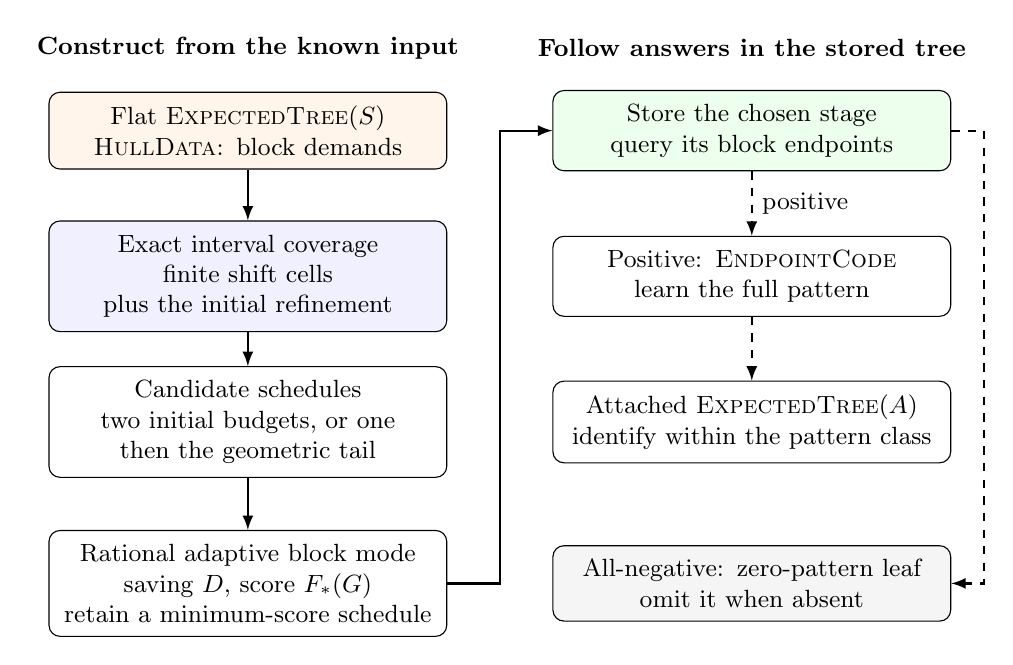
\begin{tikzpicture}[every node/.style={font=\small},
  box/.style={draw,rounded corners,align=center,inner sep=5pt,text width=4.7cm},
  arr/.style={-latex,thick},exec/.style={-latex,thick,dashed}]
  \node[font=\small\bfseries] at (-3.2,1.05) {Construct from the known input};
  \node[font=\small\bfseries] at (3.2,1.05) {Follow answers in the stored tree};
  \node[box,fill=orange!8] (hull) at (-3.2,0)
    {Flat \ExpectedTree$(S)$\\\HullData: block demands};
  \node[box,fill=blue!6] (covers) at (-3.2,-1.85)
    {Exact interval coverage\\finite shift cells\\plus the initial refinement};
  \node[box] (variants) at (-3.2,-3.7)
    {Candidate schedules\\two initial budgets, or one\\then the geometric tail};
  \node[box] (score) at (-3.2,-5.75)
    {Rational adaptive block mode\\saving $D$, score $F_*(G)$\\retain a minimum-score schedule};
  \node[box,fill=green!7] (stored) at (3.2,0)
    {Store the chosen stage\\query its block endpoints};
  \node[box] (positive) at (3.2,-1.85)
    {Positive: \EndpointCode\\learn the full pattern};
  \node[box] (child) at (3.2,-3.7)
    {Attached \ExpectedTree$(A)$\\identify within the pattern class};
  \node[box,fill=gray!8] (zero) at (3.2,-5.75)
    {All-negative: zero-pattern leaf\\omit it when absent};
  \draw[arr] (hull) -- (covers);
  \draw[arr] (covers) -- (variants);
  \draw[arr] (variants) -- (score);
  \draw[arr] (score.east) -- (0,-5.75) -- (0,0) -- (stored.west);
  \draw[exec] (stored) -- node[right]{positive} (positive);
  \draw[exec] (positive) -- (child);
  \draw[exec] (stored.east) -- (6.15,0) -- (6.15,-5.75)
    -- (zero.east);
\end{tikzpicture}
\caption{The polynomial expected-depth algorithm first computes hull
patterns and their block demands, then uses interval coverage to build
candidate schedules and selects one by its rational score. Solid arrows
show this construction-time data flow, using the supplied incidence
table and prior. The chosen stage is then stored as a query tree: dashed
arrows trace the unknown hypothesis through discovery, endpoint
decoding, and its already constructed recursive child. The adaptive
mode decides whether discovery stops at the first positive endpoint or
queries both endpoints. The algorithm makes this schedule choice
deterministically; the certificate's mixture is used to prove its cost
bound.}
\label{fig:expected-procedure-flow}
\end{figure}



The analysis follows the same separation between discovery and
pattern recovery. First we extract a benchmark from an optimal
tree. Then we bound the cost of a stage with a given schedule,
compare the chosen schedule with that benchmark, and sum stage
bounds over the recursion. The next four propositions state these
steps; their proofs follow the theorem.
Recall the binary entropy $h$ from Definition~\ref{def:entropy}, and define
\[
 \sigma(\delta)=-k_\delta\delta\ln\delta-r_\delta\ln r_\delta,
 \quad k_\delta=\lfloor1/\delta\rfloor,\quad
 r_\delta=1-k_\delta\delta,
\]
with $0\ln0=0$. The latter is the minimum entropy of a fully capped
mass distribution, including its possible remainder.

For analysis, follow the common witness through an optimal tree. Each
pattern stays on that path until a supporting hull test hits it; once
the pattern is known, its earlier queries can be omitted. The first
proposition quantifies this restriction credit and translates the
witness path into adjacent hull blocks for comparison with our schedule.
\begin{proposition}[Witness-path restriction credit]
\label{lem:support-prefix}
Follow the common witness through an optimal tree, along a path of
length $\ell$. For each pattern class $A$, let $t_A$ be the first
path query whose hull supports meet its positive pattern; put
$t_A=\ell+1$ if none do. Then
\begin{equation}\label{eq:support-prefix-credit}
 \Delta\ge\sum_{A\ne A_0}w(A)(t_A-1)+p_0\ell.
\end{equation}
The corresponding positive witness masses
$m_t=\sum_{A\ne A_0:t_A=t}w(A)$ sum to $b$ and satisfy
$m_t\le2\delta w$. An edge comparison ordering hits every positive
class by rank $t_A$. If $A_0$ exists, it covers all positive classes
with at most $\ell$ blocks, so $k_{\min}\le\ell$.
\end{proposition}

Next we price an actual stage. The rational score accounts for
discovery and endpoint-mode savings, while the information term
accounts for the remaining decoding. We deliberately retain only
a coarsened transcript: every positive cell then lies inside one
small cap, which gives a uniform entropy lower bound.

Write $W_{\rm pat}(S)$ for the original-prior expected number of
queries used by this stage to discover the full pattern and decode its
endpoints. It excludes the recursive child trees and includes the
all-negative route when the zero-pattern class is present.

\begin{proposition}[Pattern-stage cost and discovery information]
\label{prop:expected-stage}
For every candidate schedule and its selected modes, the full-pattern
stage uses only supplied queries and satisfies
\begin{equation}\label{eq:adaptive-stage}
 W_{\rm pat}(S)\le F_*(G)+3b+\frac{I-J_*}{\ln2},
 \qquad 0\le J_*\le I,
\end{equation}
where $J_*$ is the information of a coarsened discovery transcript.
Every positive coarsened exit is contained in one hull cap, and hence
\begin{equation}\label{eq:coarse-discovery-cap}
 J_*\ge b\sigma(\delta).
\end{equation}
The zero transcript is the zero-pattern singleton when it exists.
\end{proposition}

Exact coverage connects the optimal witness ranks to the actual
schedule. Proposition~\ref{prop:batch-average} bounds the average joint
score of shifted schedules, and Proposition~\ref{prop:batch-derandomization}
shows that the finite search returns one whose score is no larger than
that average. The next proposition converts this schedule comparison
into a local stage bound; its coefficient $B$ is calibrated after the
proof.
\begin{proposition}[Polynomial schedule and the local bound]
\label{prop:expected-schedule}
With the final calibration, the two-budget schedule algorithm is
polynomial in the input and rational bit length. At every flat state,
including a degenerate hull, its full-pattern stage satisfies
\begin{equation}\label{eq:two-phase-local}
 W_{\rm pat}(S)\le A\Delta+B b+\frac{I-J_*}{\ln2},
 \qquad A=\frac{\beta+1}{\ln\beta},
\end{equation}
where $B$ is the positive-mass coefficient certified in
Section~\ref{sec:two-phase}.
\end{proposition}

The local bound still contains positive mass and residual
information. The capped-transcript entropy absorbs the mass term,
leaving a charge to restriction and information decreases alone.
Those decreases telescope over the recursive pattern classes.
\begin{proposition}[Stage-to-tree conversion]\label{lem:stage-conversion}
Suppose flat stages satisfy
$W\le A\Delta+Bb+(I-J)/\ln2$ and $0\le J\le I$,
$J\ge b\sigma(\delta)$, with nonnegative $A,B$.
A recursion using those stages and mass-balanced queries has
\[
 c_{\mathrm E}(T(S))\le A\OPT_{\mathrm E}(S)+c\mathcal E(S),
 \qquad c=\max\{1/h(\delta),B/\sigma(\delta)\}.
\]
Consequently its ratio is at most $A+c\ln2$.
\end{proposition}

\begin{proofstrategy}
\textbf{Expected-depth proof roadmap.}
\begin{enumerate}
\item Replace an optimal witness query by its adjacent hull supports.
      Restriction pays for the resulting first-hit ranks.
\item Choose whether the first positive block stops early or learns
      both endpoint bits. Its recorded information reduces the
      endpoint-decoding cost.
\item Exact coverage transfers witness prefix mass to actual batches.
      A fixed certificate pays for changed initial ranks and for
      the complete zero waiting route.
\item Bound every stage by its restriction and entropy decreases,
      then telescope. Numerical tuning is deferred until after these proofs.
\end{enumerate}
\end{proofstrategy}

These propositions reduce the overall guarantee to a local schedule
bound and a final choice of constants. The theorem's proof only
combines those ingredients; the geometric, information, and
schedule arguments are established separately below.
\begin{theorem}[Polynomial expected-depth approximation]
\label{thm:two-phase-expected}
For a separating supplied family of binary unit-cost planar line
queries and arbitrary strictly positive rational priors,
\ExpectedTree\ runs in deterministic polynomial time and returns
\[
 c_{\mathrm E}(T(S))\le A\OPT_{\mathrm E}(S)+c\mathcal E(S),
 \qquad \boxed{A+c\ln2<5.182976.}
\]
Here $c=\max\{1/h(\delta),B/\sigma(\delta)\}$.
Its running-time exponent is independent of the smallest prior.
\end{theorem}
\begin{proof}
Proposition~\ref{prop:expected-schedule} gives the local stage bound;
Proposition~\ref{prop:expected-stage} gives its discovery-information
lower bound. Proposition~\ref{lem:stage-conversion} sums them over the
recursion. The calibration in Section~\ref{sec:two-phase} gives the
stated factor. Each nonsingleton stage partitions its state into
proper disjoint classes, so the polynomial stage constructions form
at most $n-1$ recursive stages.
\end{proof}

\subsection{Proofs of the supporting propositions}

\paragraph{Proof of Proposition~\ref{lem:support-prefix}.}
We first show why an unhit pattern shares the witness's optimal
prefix. This yields restriction credit directly. We then enlarge
each query's supports to an adjacent hull block, obtaining the
coverage benchmark needed by the actual scheduling algorithm.

\begin{claim}[An unhit support forces an optimal-prefix query to be constant]
\label{clm:expected-prefix-constant}
Before the first supporting hit $t_A$, every member of $A$ follows
the common witness through its first $t_A-1$ queries.
\end{claim}
\begin{proof}
All supporting hull bits of each earlier query are negative on $A$.
The cap-cover implication of Lemma~\ref{lem:hull-structure}
therefore forces that supplied query
to have the witness's answer throughout $A$. Induct along the path.
Restricting the optimal tree to $A$ contracts these constant queries,
saving at least $w(A)(t_A-1)$. To see the weighted comparison
explicitly, let $T^\circ$ be the optimal tree and let
$\pi_h$ be the original weight of hypothesis $h$. For every positive
class $A$,
\[
 \begin{aligned}
 \OPT_{\mathrm E}(A)
 &\le c_{\mathrm E}(T^\circ|_A)
   =\sum_{h\in A}\pi_h d_{T^\circ|_A}(h)\\
 &\le\sum_{h\in A}\pi_h d_{T^\circ}(h)
         -w(A)(t_A-1).
 \end{aligned}
\]
The first inequality uses feasibility of the restricted tree.
The second uses the removal of at least $t_A-1$ common queries
from every surviving path; summing their original weights gives
the credit $w(A)(t_A-1)$.
A class unhit on the entire path reaches its leaf $z$, so it is
$\{z\}$. When $A_0$ exists, this is exactly $A_0$ and its credit is
$p_0\ell$; its restricted tree has cost zero. Summing the displayed
inequality over all positive classes and including this singleton
gives
\[
 \begin{aligned}
 \sum_{A\in\Pi}\OPT_{\mathrm E}(A)
 &\le\sum_{h\in S}\pi_h d_{T^\circ}(h)
       -\sum_{A\ne A_0}w(A)(t_A-1)-p_0\ell\\
 &=\OPT_{\mathrm E}(S)
       -\sum_{A\ne A_0}w(A)(t_A-1)-p_0\ell.
 \end{aligned}
\]
The classes partition $S$, so their original depth contributions
sum to the full tree's contribution; its optimality then gives
the final equality.
Subtracting the left side from $\OPT_{\mathrm E}(S)$ proves
\eqref{eq:support-prefix-credit}. When $A_0$ is empty, its term is
zero and the same sum applies. In particular,
$\sum_{A\ne A_0}w(A)(t_A-1)=\sum_t m_t(t-1)$.
\end{proof}

The prefix credit comes from supplied queries on an optimal-tree path.
Replace each query by a full-hull edge containing its supports. This
enlargement preserves or improves its first-hit rank, so the prefix
gives a feasible comparison schedule on adjacent hull blocks.
\begin{claim}[Adjacent comparison blocks cover witness prefixes]
\label{clm:expected-comparison-blocks}
Replace each witness query by a full-hull edge containing its one or
two real supports. A singleton support may use either incident edge.
This comparison hits every class by its index $t_A$.
\end{claim}
\begin{proof}
By Lemma~\ref{lem:hull-structure}, the one or two real supports
fit in one hull edge. Enlarging the support set to that edge
cannot delay a hit. Removing
repeated or unproductive edges improves ranks further. If the terminal
singleton has a nonzero pattern and remains unhit, append an edge
incident to one of its positive vertices; its rank is at most
$\ell+1=t_A$. If $A_0$ exists, all positive classes were already hit
within the $\ell$ witness blocks, by
Claim~\ref{clm:expected-prefix-constant}. Each ordinary first-hit mass lies
in the union of the supports of that path query. Writing these caps
as $C_v,C_{v'}$, and allowing one to be absent,
\[
 m_t\le w((C_v\cup C_{v'})\cap S)
       \le w(C_v\cap S)+w(C_{v'}\cap S)\le2\delta w.
\]
The first inequality puts each rank-$t$ class in at least one
support cap. The second is the union bound, and the last uses
mass-flatness, since both hull vertices are supplied tests.
An appended terminal singleton lies in one such cap, so its mass is
at most $\delta w$. The classes partition $S\setminus A_0$, hence
$\sum_t m_t=b$. If $A_0$ exists, every positive class leaves its
optimal path before the zero leaf; the at-most-$\ell$ comparison
blocks therefore give a full cover and $k_{\min}\le\ell$.
This proves all remaining statements of the proposition. The algorithm
constructs its own order; we use the witness order only to compare costs.
\end{proof}

\paragraph{Proof of Proposition~\ref{prop:expected-stage}.}
There are three parts to the stage accounting. Count the physical
queries in each endpoint mode, credit the additional information
without counting it twice, and lower-bound the information retained
in capped discovery exits. Throughout, first-hit ranks refer to the
actual candidate schedule.

\begin{claim}[Two endpoint modes have explicit physical costs]
\label{clm:expected-mode-costs}
A positive class first hit by block $k$ has nonentropy allowance
$2k+3$. Stop mode saves $y$ weighted queries; query-both mode saves
$x+y-z$ before accounting for its additional information.
\end{claim}
\begin{proof}
At most $2(k-1)$ tests precede the hitting block. In stop mode the
first-positive route uses one discovery query and the two legal
endpoint codes of Lemmas~\ref{lem:legal-endpoint-queries}
and~\ref{lem:alphabetic-endpoints},
with overhead four. The second-positive route uses two discovery
queries, but its adjacent negative answer pins one boundary, leaving
only overhead two. Relative to $2k+3$, exactly the second endpoint's
exclusive mass $y$ saves one query. In query-both mode each exclusive
route uses two discovery queries and one endpoint code, for allowance
$2k+2$; the shared route uses two queries and two codes, for allowance
$2k+4$. Their weighted saving is $x+y-z$. A free origin endpoint or a
cached answer can only lower these costs. Finish the recorded mode
before singleton inference in the analysis, then contract constant
questions in the constructed tree.
Here are the allowances before the conditional entropy term is
added; each endpoint code contributes overhead at most two:
\[
 \begin{array}{c|c|c|c}
  \text{mode and exit}&\text{discovery}&
       \text{codes}&\text{allowance}\\\hline
  \text{stop: first positive}&1&2&2(k-1)+1+4=2k+3\\
  \text{stop: second positive}&2&1&2(k-1)+2+2=2k+2\\
  \text{both: exclusive}&2&1&2(k-1)+2+2=2k+2\\
  \text{both: shared}&2&2&2(k-1)+2+4=2k+4
 \end{array}
\]
For $m=x+y+z$, the stop allowance is consequently
\[
 (x+z)(2k+3)+y(2k+2)=(2k+3)m-y,
\]
whereas the query-both allowance is
\[
 (x+y)(2k+2)+z(2k+4)
       =(2k+3)m-(x+y-z).
\]
The zero route uses at most two tests per block, contributing
$2p_0|G|$. Summing the common positive allowance gives
$\sum_{A\ne A_0}w(A)(2k_A+3)=2\sum_{A\ne A_0}w(A)k_A+3b$.
\end{proof}

The second endpoint can reduce the information the decoder must
learn, so the stage measure accounts for both query count and
information. Temporarily forgetting that answer creates a coarsened
transcript whose entropy loss measures the benefit exactly and whose
positive cells remain inside individual caps.
\begin{claim}[Coarsening accounts for the additional information once]
\label{clm:expected-coarsening}
In a query-both block, forget the second answer on routes whose first
answer was positive. The resulting positive events lie in individual
caps, and the forgotten information pays for $E_*(a,z)$, where $a$
is the first endpoint's exclusive mass.
\end{claim}
\begin{proofstrategy}
\begin{enumerate}
\item Compute the entropy loss from merging the two events and use the
      calibrated entropy tent to lower-bound it by $E_*(a,z)$.
\item Express endpoint-code entropy as the information left after
      discovery, then compare the actual and coarsened transcripts.
\item Combine that information difference with the physical mode
      savings, so each block's saving is charged once in
      \eqref{eq:adaptive-stage}.
\end{enumerate}
\end{proofstrategy}
\begin{proof}
The coarsening merges masses $a,z$ inside the first endpoint's cap;
the other exclusive event lies in the second endpoint's cap.
Using the same total state mass $w$ before and after the merge,
the weighted information loss is
\[
 \begin{aligned}
 \mathcal L(a,z)
 &=-a\ln(a/w)-z\ln(z/w)+(a+z)\ln((a+z)/w)\\
 &=a\ln\frac{a+z}{a}+z\ln\frac{a+z}{z}
   =(a+z)h\!\left(\frac a{a+z}\right).
 \end{aligned}
\]
The first equality cancels the common normalization terms
in $\ln w$. For the second, substitute the two conditional
probabilities $a/(a+z)$ and $z/(a+z)$ into binary entropy.
Terms of zero mass have value zero, and $\mathcal L(0,0)=0$.
To justify the entropy tent, first take $0\le v\le p_*$. Concavity
between $0$ and $p_*$ gives
$H_2(v)\ge(v/p_*)H_2(p_*)\ge(h_*/p_*)v$.
On $[p_*,1-p_*]$, concavity between the two equal endpoint
entropies gives $H_2(v)\ge H_2(p_*)\ge h_*$.
On $[1-p_*,1]$, symmetry gives
$H_2(v)\ge(h_*/p_*)(1-v)$. These three inequalities prove
\[
 H_2(v)\ge\min\{(h_*/p_*)v,\ h_*,\ (h_*/p_*)(1-v)\},
\]
provided the calibration satisfies $H_2(p_*)\ge h_*$.
For $v=a/(a+z)$, multiplying by $a+z$ therefore gives
\[
 \frac{\mathcal L(a,z)}{\ln2}
 =(a+z)H_2\!\left(\frac a{a+z}\right)
 \ge\min\{(h_*/p_*)a,h_*(a+z),(h_*/p_*)z\}
 =E_*(a,z).
\]

Let $\mathcal D_{\rm act}$ be the actual discovery partition and
$J_{\rm act}$ its weighted information. On an exit $B$, learn the
left endpoint $U$ and then the right endpoint $V$ conditioned on
$U$ and $B$. The endpoint pair and the full pattern determine
each other. Thus Lemma~\ref{lem:entropy-chain-rule} makes the
entropy part of the expected code lengths supplied by
Lemma~\ref{lem:alphabetic-endpoints} equal to
\[
 \frac{w(B)}{\ln2}\bigl[H(U\mid B)+H(V\mid U,B)\bigr]
 =\frac{w(B)}{\ln2}H(\Pi\mid B).
\]
A pinned endpoint is constant and has entropy zero; its code and
overhead are omitted. Summing over exits, including the zero exit
whose pattern is already known, Lemma~\ref{lem:entropy-chain-rule} gives
\[
 \sum_{B\in\mathcal D_{\rm act}}w(B)H(\Pi\mid B)
 =wH(\Pi)-wH(\mathcal D_{\rm act})=I-J_{\rm act}.
\]
Here the conditional entropies use the normalized weights within
each exit, while the prefactors preserve the original weights.
The discovery label is determined by the full pattern, so its
entropy is exactly the information already removed from the
remaining pattern entropy. The final equality uses the definitions
of $I$ and $J_{\rm act}$.

Let $\mathcal Q$ be the blocks using query-both mode, with physical
weighted savings $P_g=x_g+y_g-z_g$; for stop blocks put $P_g=y_g$.
Claim~\ref{clm:expected-mode-costs} and this conditional-entropy sum give
\[
 W_{\rm pat}(S)\le
 2\sum_{A\ne A_0}w(A)k_A+2p_0|G|+3b
 -\sum_gP_g+\frac{I-J_{\rm act}}{\ln2}.
\]
Write $\mathcal D_*$ for the resulting coarsened partition.
The merged exits are disjoint across blocks, so
$J_{\rm act}-J_*=\sum_{g\in\mathcal Q}\mathcal L(a_g,z_g)$.
Indeed, each merge changes only its two positive exit cells,
so the separate entropy losses add. Substituting this identity gives
\[
 \begin{aligned}
 -\sum_gP_g+\frac{I-J_{\rm act}}{\ln2}
 &=\frac{I-J_*}{\ln2}
   -\sum_{g\notin\mathcal Q}y_g\\
 &\quad-\sum_{g\in\mathcal Q}
       \left(x_g+y_g-z_g+\frac{\mathcal L(a_g,z_g)}{\ln2}\right)\\
 &\le\frac{I-J_*}{\ln2}-\sum_gD(x_g,y_g,z_g).
 \end{aligned}
\]
The last inequality uses the chosen mode and
$\mathcal L(a_g,z_g)/\ln2\ge E_*(a_g,z_g)$, with $a_g=y_g$.
Thus the lost information is subtracted exactly once. Because
each of the three linear forms in
$E_*(a,z)$ is nondecreasing in $a$, asking the larger exclusive mass
first maximizes this credit. In stop mode, ask the smaller exclusive
mass first. The displayed cost inequality is now precisely
\eqref{eq:adaptive-stage}, after inserting the definition of $F_*(G)$.
\end{proof}

We now need a lower bound on the retained discovery information
that works even when the zero-pattern singleton has large mass.
All positive exits are capped; the zero exit is the sole
unrestricted one. Concentrating the capped masses as much as
possible identifies the least informative such transcript.
\begin{claim}[Capped discovery exits have entropy proportional to positive mass]
\label{lem:capped-discovery-entropy}
A probability vector with one unrestricted entry $p_0$ and all
remaining entries at most $\delta$ has entropy at least
$(1-p_0)\sigma(\delta)$.
\end{claim}
\begin{proofstrategy}
\begin{enumerate}
\item Use entropy-decreasing mass transfers to reduce a minimizer to
      entries packed at the cap, with at most one remainder.
\item On each interval with a fixed number of capped entries, show the
      packed entropy minus $b\sigma(\delta)$ is concave.
\item Check the interval endpoints using the packed-mass ratios; the
      chord bound then gives the claim throughout each interval.
\end{enumerate}
\end{proofstrategy}
\begin{proof}
Put $f(a)=-a\ln a$ with $f(0)=0$, and let $b=1-p_0$.
Moving mass from a smaller capped entry to a larger one cannot
increase entropy: if $a\ge c>0$ and
$0\le\epsilon\le\min\{\delta-a,c\}$, then
\[
 \frac{d}{d\epsilon}
 \bigl[f(a+\epsilon)+f(c-\epsilon)\bigr]
 =\ln\frac{c-\epsilon}{a+\epsilon}\le0.
\]
Transfer until one entry is zero or the other reaches its cap.
Repeating leaves at most one positive entry below $\delta$, giving
the minimum
shape: $j=\lfloor b/\delta\rfloor$ entries of mass $\delta$ and
one possible remainder. Its total entropy is
\[
 T(b)=f(1-b)+j f(\delta)+f(b-j\delta).
\]
On each interval with fixed $j$, the only varying terms are
$f(1-b)+f(b-j\delta)$, and
\[
 T''(b)=-\frac1{1-b}-\frac1{b-j\delta}<0
\]
in its interior. Thus $T(b)-b\sigma(\delta)$ is concave there.
It suffices to check $T(b)\ge b\sigma(\delta)$ at those
multiples and at $0,1$. At $b=j\delta>0$,
\[
 T(b)/b=L+g(1-b),\quad L=\ln(1/\delta),\quad
 g(a)=\frac{-a\ln a}{1-a}.
\]
Differentiating the quotient gives
\[
 g'(a)=\frac{(-\ln a-1)(1-a)-a\ln a}{(1-a)^2}
      =\frac{-\ln a-1+a}{(1-a)^2}\ge0,
\]
where $\ln a\le a-1$ proves the sign. These ratios decrease
as $b$ increases. If the final remainder $r_\delta=1-\lfloor1/\delta\rfloor\delta$
is zero, the last ratio is $L=\sigma(\delta)$. Otherwise its
excess over $T(1)=\sigma(\delta)$ is, writing $r=r_\delta$,
\[
 \begin{aligned}
 \left[L+\frac{f(r)}{1-r}\right]
     -\bigl[(1-r)L+f(r)\bigr]
 &=rL+\frac{r f(r)}{1-r}\ge0.
 \end{aligned}
\]
The last sign uses $r,L,f(r)\ge0$ and $r<1$. Consequently
every multiple has nonnegative excess, while
$T(0)=0$ and $T(1)=\sigma(\delta)$. A concave function lies above
the chord between its endpoints, so the required inequality holds
on every intervening interval. Also
$\sigma(\delta)=\ln(1/\delta)+r_\delta\ln(\delta/r_\delta)
\ge\ln(1/\delta)$,
because $0<r_\delta<\delta$ when the remainder is positive;
the second term is zero at $r_\delta=0$.
\end{proof}
By Claim~\ref{clm:expected-coarsening}, every nonzero coarsened
discovery cell lies in a cap of mass below
$\delta w$. Its normalized zero mass is $p_0/w$, so the claim gives
\[
 J_*=wH(\mathcal D_*)\byref{Claim}{lem:capped-discovery-entropy}{\ge}
      w\left(1-\frac{p_0}{w}\right)\sigma(\delta)
      =b\sigma(\delta).
\]
This is \eqref{eq:coarse-discovery-cap}. The transcript is a function
of the full pattern, so Lemma~\ref{lem:entropy-chain-rule} gives
$I=J_*+wH(\Pi\mid\mathcal D_*)\ge J_*$; entropy nonnegativity
also gives $J_*\ge0$. Endpoint recovery identifies
the complete pattern, while a negative full cover identifies $A_0$.
This finishes Proposition~\ref{prop:expected-stage}.

\paragraph{Proof of Proposition~\ref{prop:expected-schedule}.}
The next claims separate actual coverage and mode savings from their
optimal-witness comparison. Actual first-hit ranks price the constructed
schedule; witness ranks provide restriction credit. Exact coverage is
the connection between them.

The exact mode saving depends on how a block's mass is split between
its endpoints. For a batch comparison we need bounds depending only
on its total newly hit mass and the cap size. Two affine minorants
of the saving provide that simpler form.
\begin{claim}[Block mode savings have two affine lower bounds]
\label{lem:affine-block-credit}
For newly hit mass $m=x+y+z$, with endpoint caps bounded by
$\delta w$, the selected saving satisfies
\[
 D\ge0,\qquad D\ge m-\delta w,\qquad
 D\ge c_*m-d_*\delta w,
 \quad c_*=\frac{2-p_*}{1-p_*},\quad d_*=\frac2{1-p_*}.
\]
\end{claim}
\begin{proof}
Stop mode gives $D\ge y\ge0$ and $m-y=x+z\le\delta w$.
These are the first two bounds, by the definition
\eqref{eq:rational-block-saving} and the first endpoint's cap bound.
For the last inequality normalize $\delta w=1$; the saving is
homogeneous because every term in $E_*$ and $D$ is linear before
taking minima or maxima. It is immediate
if $m\le1$, because $c_*m-d_*\le c_*-d_*=-p_*/(1-p_*)<0$.
The two cap bounds imply $m+z=(x+z)+(y+z)\le2$, so no mass
$m>2$ is feasible. For $1\le m\le2$, substitute $z=m-x-y$.
The cap inequalities and
the chosen endpoint order become
\[
 x\ge m-1,\qquad y\ge m-1,\qquad x\le y,\qquad x+y\le m.
\]
Specifically, $y+z\le1$ gives $x\ge m-1$, $x+z\le1$
gives $y\ge m-1$, and $z\ge0$ gives $x+y\le m$.
Thus the feasible $(x,y)$ triangle has
vertices $(m-1,m-1)$, $(m-1,1)$, and $(m/2,m/2)$.
The concave expression $x+y-z+E_*(x,z)$ is a lower bound on the
selected query-both saving, since $E_*(y,z)\ge E_*(x,z)$.
Concavity follows because, after substituting $z$, it is a linear
term plus the minimum of three affine functions. The selected
saving $D$ dominates it by \eqref{eq:rational-block-saving}.
At the two vertices with $z=0$ it equals $m$; at the other it is
\[
 f(m)=3m-4+\min\{(h_*/p_*)(m-1),\ h_*,\ (h_*/p_*)(2-m)\}.
\]
For $m\le1+p_*$, $c_*m-d_*\le m-1$, already covered by stop mode.
Indeed,
\[
 c_*m-d_*-(m-1)=\frac{m-1-p_*}{1-p_*}\le0.
\]
On $[1+p_*,2]$, the minimum of the three affine terms makes $f$
concave. Since $h_*=1-2p_*$ and $p_*<1/2$,
\[
 \begin{aligned}
 f(1+p_*)&=-1+3p_*+
   \min\{h_*,h_*,h_*(1-p_*)/p_*\}=p_*,\\
 f(2)&=2+\min\{h_*/p_*,h_*,0\}=2.
 \end{aligned}
\]
The chord between these endpoints is
\[
 p_*+\frac{2-p_*}{1-p_*}(m-1-p_*)
 =\frac{(2-p_*)m-2}{1-p_*}=c_*m-d_*.
\]
At the other two triangle vertices the value $m$ also dominates
this chord, because
$m-(c_*m-d_*)=(2-m)/(1-p_*)\ge0$.
For fixed $m$, every feasible point is a convex combination of
the triangle vertices. Concavity therefore bounds its query-both
saving below by the same chord. Restoring the scale $\delta w$
multiplies both $m$ and the saving by that scale, proving the last
affine bound.
\end{proof}

The witness's first $q$ blocks cover a known amount of comparison
mass. Exact budgeted coverage must cover at least that amount,
although it may choose entirely different blocks. Summing either
affine minorant over the chosen batch therefore transfers witness
prefix mass into an actual mode-saving guarantee.
\begin{claim}[Exact first-batch coverage transfers witness prefix mass]
\label{clm:expected-first-batch-credit}
Let $M_q=\sum_{t\le q}m_t$. A first budget-$q$ batch gives total
schedule savings at least each of
\[
 \mathsf A_q=M_q-\delta wq,\qquad
 \mathsf C_q=c_*M_q-d_*\delta wq,\qquad 0.
\]
\end{claim}
\begin{proof}
By Claim~\ref{clm:expected-comparison-blocks}, the witness comparison
covers $M_q$ using at most $q$ blocks. Thus
Lemma~\ref{lem:budget-coverage} selects a set covering mass at least
$M_q$. Let its productive blocks have newly hit masses
$\widehat m_1,\ldots,\widehat m_h$, where $h\le q$ and
$\sum_i\widehat m_i\ge M_q$. The two sums are explicitly
\[
 \begin{aligned}
 \sum_{i=1}^hD_i
 &\byref{Claim}{lem:affine-block-credit}{\ge}\sum_{i=1}^h(\widehat m_i-\delta w)
   =\sum_i\widehat m_i-h\delta w
   \ge M_q-q\delta w,\\
 \sum_{i=1}^hD_i
 &\byref{Claim}{lem:affine-block-credit}{\ge}\sum_{i=1}^h(c_*\widehat m_i-d_*\delta w)
   =c_*\sum_i\widehat m_i-d_*h\delta w
   \ge c_*M_q-d_*q\delta w.
 \end{aligned}
\]
Here $c_*,d_*>0$, so replacing the covered mass by its lower bound
and the number of blocks by its upper bound has the stated signs.
All subsequent mode savings are nonnegative by
Claim~\ref{lem:affine-block-credit}, so both batch bounds also
bound the complete schedule's saving.
If $q\ge k_{\min}$, the minimum cover hits all positive
mass with at most $q$ blocks, so $\sum_i\widehat m_i=b\ge M_q$
and the same calculation holds. If coefficients
$\theta_A,\theta_C,\theta_0\ge0$ sum to one, then
$\theta_A\mathsf A_q+\theta_C\mathsf C_q+\theta_0\cdot0$
is also at most the one total saving, because each of its three
terms is a lower bound on that same saving.
\end{proof}

Changing the first budgets can help early hits and hurt later ones.
It can also change how long the zero hypothesis waits before a
full cover finishes. We keep both changes with their signs; this
prevents an improvement for common positive patterns from hiding
an increased cost on the all-negative route.
\begin{claim}[Changing the initial budgets has signed first-hit and zero-route costs]
\label{clm:expected-initial-budget-correction}
Relative to the geometric sequence $k_0,k_1,k_2,\ldots$, the exact
doubled first-hit improvement is
\begin{equation}\label{eq:two-phase-correction}
 \begin{aligned}
 d_{q,r}(u,t)={}&k_0-q+(k_0+k_1)\mathbf1_{\{t>k_0\}}
                    +(k_1+k_2)\mathbf1_{\{t>k_1\}}\\
 &-(q+r)\mathbf1_{\{t>q\}}-(r+k_2)\mathbf1_{\{t>r\}},\quad r>0,\\
 d_{q,0}(u,t)={}&k_0-q+(k_0+k_1)\mathbf1_{\{t>k_0\}}
                    +(k_1+k_2)\mathbf1_{\{t>k_1\}}\\
 &-(q+k_2)\mathbf1_{\{t>q\}}.
 \end{aligned}
\end{equation}
The full all-negative length invoice changes by
\begin{equation}\label{eq:two-phase-zero-correction}
 z_{q,r}(u,k)=q\mathbf1_{\{q<k\}}+r\mathbf1_{\{r<k\}}
             -k_0\mathbf1_{\{k_0<k\}}-k_1\mathbf1_{\{k_1<k\}},
 \qquad k=k_{\min}.
\end{equation}
\end{claim}
\begin{proof}
The within-batch bound of Claim~\ref{clm:batch-first-cover},
together with phase coverage from Claim~\ref{clm:batch-phase-cover}, bounds
first-hit cost for any increasing budgets $a_0,a_1,\ldots$ by
\[
 \frac{a_0+1}{2}
 +\frac12\sum_{j\ge0}(a_j+a_{j+1})\mathbf1_{\{t>a_j\}}.
\]
Write $\mathcal B_{\rm old}(u,t)$ and
$\mathcal B_{q,r}(u,t)$ for these invoices. If
$\mathcal T(u,t)=\sum_{j\ge2}(k_j+k_{j+1})\mathbf1_{\{t>k_j\}}$,
their doubled values are
\[
 \begin{aligned}
 2\mathcal B_{\rm old}
 &=k_0+1+(k_0+k_1)\mathbf1_{\{t>k_0\}}
       +(k_1+k_2)\mathbf1_{\{t>k_1\}}+\mathcal T,\\
 2\mathcal B_{q,r}
 &=q+1+(q+r)\mathbf1_{\{t>q\}}
       +(r+k_2)\mathbf1_{\{t>r\}}+\mathcal T\quad(r>0),\\
 2\mathcal B_{q,0}
 &=q+1+(q+k_2)\mathbf1_{\{t>q\}}+\mathcal T.
 \end{aligned}
\]
Subtracting cancels the common $1$ and $\mathcal T$, giving
$2(\mathcal B_{\rm old}-\mathcal B_{q,r})=d_{q,r}(u,t)$.
Every coefficient in $\mathcal B_{q,r}$ is nonnegative. Hence
this invoice is nondecreasing in $t$, and comparison edges that
hit earlier than $t_A$, as allowed by
Claim~\ref{clm:expected-comparison-blocks}, only improve the bound.
Early completion removes nonnegative continuation terms. For the
negative route and $k=k_{\min}$, the full budget invoices are
\[
 \begin{aligned}
 \mathcal L_{\rm old}(u,k)
 &=k+k_0\mathbf1_{\{k_0<k\}}+k_1\mathbf1_{\{k_1<k\}}
        +\sum_{j\ge2}k_j\mathbf1_{\{k_j<k\}},\\
 \mathcal L_{q,r}(u,k)
 &=k+q\mathbf1_{\{q<k\}}+r\mathbf1_{\{r<k\}}
        +\sum_{j\ge2}k_j\mathbf1_{\{k_j<k\}}.
 \end{aligned}
\]
The final minimum cover contributes the same $k$; a budget below
$k$ contributes at most its full size. Subtracting now cancels both
the final cover and the common tail, so
$\mathcal L_{q,r}-\mathcal L_{\rm old}=z_{q,r}(u,k)$.
The $r$ term is zero for $r=0$. If an initial budget already reaches
$k$, all later budgets are larger and their indicators vanish,
so this formula also includes early minimum-cover completion.
Neither change is assumed nonnegative.
\end{proof}

After averaging schedules, each witness rank will have a credit
coefficient. Most coefficients meet a common threshold, and the
cap bound limits the mass at any exceptional rank. The next
calculation combines these facts without assuming that all mass
is positive: its final term explicitly retains the zero prior.
\begin{claim}[One capped-mass calculation includes the zero prior]
\label{lem:capped-rank-credit}
Suppose $\sum_t m_t=b$, $m_t\le2\delta w$, and coefficients $a_t$
are at least $\tau$ except on a finite set $E$. Define
\[
 \chi=\tau-2\delta\sum_{t\in E}(\tau-a_t)_+-\delta\mu.
\]
If $\chi+\zeta\ge\tau$, then
\begin{equation}\label{eq:capped-rank-conversion}
 \sum_t m_t a_t-\delta w\mu+\zeta p_0\ge\chi b.
\end{equation}
\end{claim}
\begin{proof}
Only coefficients below $\tau$ need their individual mass caps.
Let $\varepsilon_t=(\tau-a_t)_+$ for $t\in E$, and put it equal
to zero elsewhere. Then $a_t\ge\tau-\varepsilon_t$, so
\[
 \begin{aligned}
 \sum_t m_ta_t
 &\ge\tau\sum_t m_t-\sum_{t\in E}m_t\varepsilon_t\\
 &\ge\tau b-2\delta w\sum_{t\in E}\varepsilon_t.
 \end{aligned}
\]
Subtract $\delta w\mu$ and add $\zeta p_0$. By the definition
of $\chi$, $2\delta\sum_{t\in E}\varepsilon_t+\delta\mu
=\tau-\chi$, so the result is at least
\[
 \tau b-(\tau-\chi)w+\zeta p_0
 =\chi b+p_0(\chi+\zeta-\tau)\ge\chi b.
\]
The equality uses $w=b+p_0$; the final sign uses
$p_0\ge0$ and $\chi+\zeta\ge\tau$.
This argument permits arbitrary zero-pattern mass and uses no
identification of witness ranks with actual discovery ranks.
\end{proof}

\paragraph{Assembling the local bound.}
We now combine three credits against the discovery score: the
geometric schedule's discount relative to its linear restriction
bound, the signed benefit of changing its initial budgets, and
the first batch's endpoint-mode saving. The certificate records
only their coefficients; it is not used to choose a schedule at
runtime. We describe this combination symbolically here and
defer every numerical check to Section~\ref{sec:two-phase}.

Retain $\Phi_\beta,Z_\beta,\lambda_\beta,\nu_\beta$ from the
geometric-batch lemma. Define the nondecreasing discrete discount
\[
 e_\beta(t)=2[\lambda_\beta(t-1)+\Phi_\beta(1)-\Phi_\beta(t)]
 =\frac1{\ln\beta}\int_1^t
   \left[\beta+1-\frac{\lfloor x\rfloor+\lfloor\beta x\rfloor}{x}\right]dx.
\]
The integral identity follows from the definition of $\Phi_\beta$
and $2\lambda_\beta=(\beta+1)/\ln\beta$. Its integrand is
nonnegative because each floor is at most its argument, so
$e_\beta$ is nondecreasing. Proposition~\ref{lem:support-prefix}
provides the comparison ranks. Log-uniform averaging of the old
first-hit bound gives $\Phi_\beta(t)$ by
Proposition~\ref{prop:batch-average};
Claim~\ref{clm:expected-initial-budget-correction} subtracts
$d_{q,r}(u,t)/2$ from that invoice. The same claim makes the
zero length bound at most
$Z_\beta(k_{\min})+\mathbb E[z_{q,r}(u,k_{\min})]$.

The first credit is $e_\beta(t)$ above. The other two credits
depend on the selected initial budgets and minorant, so average
them using the fixed distribution in
Section~\ref{sec:two-phase-certificate}. This distribution
compares only valid two-budget variants and first-batch minorants.
Its coefficient definition is
\begin{equation}\label{eq:two-phase-coefficients}
 a_t=e_\beta(t)+\mathbb E[d_{q,r}(u,t)+s\mathbf1_{\{t\le q\}}],
 \qquad \mu=\mathbb E[\rho],
\end{equation}
where the selected minorant is $sM_q-\rho\delta w$.
Claim~\ref{clm:expected-first-batch-credit} bounds the saving of
each selected schedule by its selected minorant. Consequently
\[
 \begin{aligned}
 &\sum_t m_t e_\beta(t)+
 \mathbb E\left[\sum_t m_t d_{q,r}(u,t)+
                  \sum_{\text{blocks of }G}D\right]\\
 &\quad\ge\sum_t m_t e_\beta(t)+
   \mathbb E\left[\sum_t m_t d_{q,r}(u,t)
                 +s\sum_{t\le q}m_t-\rho\delta w\right]\\
 &\quad=\sum_t m_t\left[e_\beta(t)
       +\mathbb E\bigl(d_{q,r}(u,t)+s\mathbf1_{\{t\le q\}}\bigr)\right]
           -\delta w\mathbb E[\rho]\\
 &\quad=\sum_t m_ta_t-\delta w\mu.
 \end{aligned}
\]
The first inequality substitutes that minorant. The next equality
uses $M_q=\sum_t m_t\mathbf1_{\{t\le q\}}$ and moves the fixed
witness masses through expectation; the last uses
\eqref{eq:two-phase-coefficients}. The witness masses $m_t$ are
fixed independently of the shift. Thus the schedule's saving is
credited once before taking expectations.
It remains to check that this combined credit is sufficient at
every rank and that the zero waiting route has not become longer
on average. The final calibration proves three conditions: all $a_t$
except $a_1$ exceed $\tau$ while $a_1<\tau$; every mean zero-length change is
nonpositive; and $\chi+2/\ln\beta\ge\tau$, where
\begin{equation}\label{eq:two-phase-chi-B}
 \chi=\tau-2\delta(\tau-a_1)-\delta\mu,\qquad
 B=3+2\Phi_\beta(1)-\chi.
\end{equation}
It also gives $\lambda_\beta\ge\nu_\beta$.
To make the score comparison explicit, write
$S(G)=\sum_{\text{blocks of }G}D$ and
$D_0(k)=\mathbb E[z_{q,r}(u,k)]$. The modified first-hit and length
invoices give
\[
 \begin{aligned}
 \mathbb E\left[\sum_{A\ne A_0}w(A)k_A\right]
 &\le\sum_t m_t\Phi_\beta(t)
          -\frac12\mathbb E\left[\sum_t m_t d_{q,r}(u,t)\right],\\
 \mathbb E[|G|]&\le Z_\beta(k_{\min})+D_0(k_{\min}).
 \end{aligned}
\]
The marginal shift law is log-uniform, so averaging the old invoice
gives $\Phi_\beta$ and $Z_\beta$ even though the conditional choice
of initial budgets depends on the shift. Insert these inequalities
in $F_*(G)$, use $D_0(k_{\min})\le0$ and $p_0\ge0$, and expand
$2\Phi_\beta(t)=2\lambda_\beta(t-1)+2\Phi_\beta(1)-e_\beta(t)$:
\[
 \begin{aligned}
 \mathbb E[F_*(G)]
 &\le2\sum_t m_t\Phi_\beta(t)+2p_0Z_\beta(k_{\min})
       -\mathbb E\left[\sum_t m_t d_{q,r}(u,t)+S(G)\right]\\
 &=2\lambda_\beta\sum_t m_t(t-1)+2\Phi_\beta(1)b
       +2p_0Z_\beta(k_{\min})\\
 &\qquad-\sum_t m_t e_\beta(t)
       -\mathbb E\left[\sum_t m_t d_{q,r}(u,t)+S(G)\right]\\
 &\byref{Eq.}{eq:two-phase-coefficients}{\le}2\lambda_\beta\sum_t m_t(t-1)+2\Phi_\beta(1)b
       +2p_0Z_\beta(k_{\min})-\sum_t m_ta_t+\delta w\mu.
 \end{aligned}
\]
If $p_0>0$, Proposition~\ref{lem:support-prefix} gives
$k_{\min}\le\ell$.
Since $\nu_\beta\le\lambda_\beta$,
\[
 2p_0Z_\beta(k_{\min})
 \byref{Prop.}{prop:batch-average}{\le}2p_0\left(\nu_\beta k_{\min}-\frac1{\ln\beta}\right)
 \le2\lambda_\beta p_0\ell-\frac{2p_0}{\ln\beta}.
\]
The second inequality uses $k_{\min}\le\ell$,
$\nu_\beta\le\lambda_\beta$, and the nonnegative factors
$p_0,\nu_\beta,\lambda_\beta$.
When $p_0=0$ these terms vanish, so no relation between
$k_{\min}$ and $\ell$ is needed. Finally,
\[
 2\lambda_\beta\left[\sum_t m_t(t-1)+p_0\ell\right]
 \byref{Prop.}{lem:support-prefix}{\le}2\lambda_\beta\Delta=A\Delta.
\]
Substitution gives
\[
 \mathbb E[F_*(G)]\le A\Delta+2\Phi_\beta(1)b
       -\sum_t m_t a_t+\delta w\mu-\frac{2p_0}{\ln\beta}.
\]
The zero credit is retained in the last term of this inequality.
The capped-mass claim with $E=\{1\}$ and $\zeta=2/\ln\beta$
gives
\[
 \sum_t m_ta_t-\delta w\mu+\frac{2p_0}{\ln\beta}\byref{Claim}{lem:capped-rank-credit}{\ge}\chi b,
 \qquad
 \mathbb E[F_*(G)]\le A\Delta+(2\Phi_\beta(1)-\chi)b.
\]
For the selected schedule $\widehat G$, minimality gives
$F_*(\widehat G)\le\mathbb E[F_*(G)]$.
The expectation averages scores of valid candidates, so their
minimum is no greater than that average.
Applying the pattern-stage proposition to its own transcript,
\[
 \begin{aligned}
 W_{\rm pat}(S)
 &\byref{Prop.}{prop:expected-stage}{\le}F_*(\widehat G)+3b+\frac{I-J_*}{\ln2}\\
 &\le A\Delta+
       \underbrace{(3+2\Phi_\beta(1)-\chi)}_{B}b
       +\frac{I-J_*}{\ln2},
 \end{aligned}
\]
which proves \eqref{eq:two-phase-local}.

Finally, the averaging argument must describe schedules the
algorithm actually tries. Shift cells give a finite family of
representatives, including when a small initial budget completes
the cover early. Hulls with too few tests for the block argument
are handled directly and satisfy the same local bound.
\begin{claim}[Degenerate hulls and finite shift enumeration preserve the bound]
\label{clm:expected-finite-enumeration}
The direct stage and the finite shift family are polynomial,
including all terminal cases.
\end{claim}
\begin{proof}
With at most two real extreme hull tests, query them directly to
learn the full pattern, at cost at most $2w$. In a nonsingleton state
with $p_0>0$, the witness path has $\ell\ge1$, so
Proposition~\ref{lem:support-prefix} gives $\Delta\ge p_0$;
otherwise $b=w$. The calibrated $A,B>2$ imply
\[
 2w=2b+2p_0\le Bb+Ap_0\le Bb+A\Delta,
\]
where $\Delta\ge0=p_0$ if the zero class is absent. Here $J_*=I$,
so the residual-information term is zero.

For a nondegenerate hull, all coverage calls are polynomial interval
DPs by Lemmas~\ref{lem:minimum-interval-cover}
and~\ref{lem:budget-coverage}. Proposition~\ref{prop:batch-derandomization}
gives polynomially many geometric shift cells;
\eqref{eq:initial-shift-refinement} adds only a constant number.
More explicitly, for any fixed $\beta>1$, there are
$O(\log k_{\min})$ geometric scales, and for each integer $k$ at most
one exponent places $k/\beta^j$ in $[1,\beta)$. The initial
refinement adds at most $2\lceil\beta^3\rceil$ breakpoints, a
constant for fixed $\beta$. The algorithm enumerates each breakpoint
and one interior representative per cell; all such representatives
give the same integer budgets within the cell.
Within a refined cell every executed budget, candidate order, mode,
and score is fixed. Thus every schedule in the proof average has an
actual enumerated representative. There are at most twenty-four
variants per cell. Prior weights enter only sums and comparisons: for
rational input priors, a sum of at most $n$ input values has
a denominator dividing the product of their denominators and
therefore has polynomial encoding length. The fixed rational
coefficients in $E_*$, $D$, and $F_*$ preserve that bound.
No logarithm or proof distribution is computed.
Empty positive demands occur only at a terminal singleton. Early
inferences, cached questions, free origin markers, and empty branches
can only reduce the constructed cost.
\end{proof}
This completes Proposition~\ref{prop:expected-schedule}.

\paragraph{Proof of Proposition~\ref{lem:stage-conversion}.}
We use one charge for both kinds of recursive step. A balanced
query already earns enough information to pay for itself. A flat
stage earns restriction credit as well, and its capped discovery
information absorbs the positive-mass term. Once both steps have
this form, summing over the recursion requires no further
geometric or scheduling argument.

\begin{claim}[Each stage is paid for by two potential decreases]
\label{clm:stage-paid}
Every balanced query or flat stage costs at most $A\Delta+cI$.
\end{claim}
\begin{proof}
A balanced query has information at least $w(S)h(\delta)$,
because its normalized side mass lies in $[\delta,1-\delta]$ and
the concave, symmetric binary entropy is minimized there at an
endpoint. Thus
\[
 W=w(S)\overset{I\ge w(S)h(\delta)}{\le}\frac{I}{h(\delta)}
 \le cI\byref{Lem.}{lem:restriction}{\le} A\Delta+cI;
\]
the final step uses $A\ge0$ and the nonnegative restriction credit.
Also Lemma~\ref{lem:entropy-chain-rule} gives $h(\delta)\le\ln2$,
so $c\ge1/h(\delta)\ge1/\ln2$.
For a flat stage, $J\ge b\sigma(\delta)$ and
$c\ge B/\sigma(\delta)$ give $Bb\le cJ$. Since $I-J\ge0$,
\[
 \begin{aligned}
 W&\overset{\text{assumed flat-stage bound}}{\le} A\Delta+Bb+\frac{I-J}{\ln2}\\
  &\le A\Delta+cJ+c(I-J)=A\Delta+cI.
 \end{aligned}
\]
The second inequality substitutes $Bb\le cJ$ and
$1/\ln2\le c$; the latter can multiply $I-J$ without changing
the inequality because $I-J\ge0$. The last equality then
recombines the information already learned and the information
still needed. Thus the argument uses only this proposition's
assumptions, and applies to any stages satisfying them.
\end{proof}

Each stage partitions its current state into the classes on which
the recursion continues. Thus the two local credits are decreases
of the same potentials before and after that partition. Summing
them cancels all internal-state terms and leaves only the root's
optimal expected cost and entropy.
\begin{claim}[Restriction and information telescope over pattern classes]
\label{clm:stage-telescoping}
The sum of stage costs is at most
$A\OPT_{\mathrm E}(S)+c\mathcal E(S)$.
\end{claim}
\begin{proof}
By their definitions,
\[
 \Delta=\OPT_{\mathrm E}(S)-\sum_{A\in\Pi}\OPT_{\mathrm E}(A),
 \qquad I=\mathcal E(S)-\sum_{A\in\Pi}\mathcal E(A).
\]
Let $\mathcal V$ be the nonsingleton recursive states and
$\mathcal L$ their singleton leaves. As in
Proposition~\ref{prop:potential-cancellation}, every nonroot state occurs
once as a child, so the internal terms cancel exactly:
\[
 \begin{aligned}
 \sum_{V\in\mathcal V}\Delta(V)
 &=\sum_{V\in\mathcal V}\OPT_{\mathrm E}(V)
   -\sum_{V\in\mathcal V}\sum_{A\in\Pi_V}\OPT_{\mathrm E}(A)\\
 &=\OPT_{\mathrm E}(S)-\sum_{A\in\mathcal L}\OPT_{\mathrm E}(A),\\
 \sum_{V\in\mathcal V}I(V)
 &=\mathcal E(S)-\sum_{A\in\mathcal L}\mathcal E(A).
 \end{aligned}
\]
Both leaf sums vanish. Each query belongs to one stage, with its
original reach mass, so summing the previous claim gives
\[
 c_{\mathrm E}(T(S))\le\sum_{V\in\mathcal V}W(V)
 \byref{Claim}{clm:stage-paid}{\le} A\OPT_{\mathrm E}(S)+c\mathcal E(S).
\]
Finally Lemma~\ref{lem:restriction}, proved by
Claim~\ref{clm:restriction-2}, gives the binary-tree entropy lower bound
$\mathcal E(S)\le\ln2\,\OPT_{\mathrm E}(S)$; substituting it yields
\[
 c_{\mathrm E}(T(S))
 \byref{Claim}{clm:restriction-2}{\le}(A+c\ln2)\OPT_{\mathrm E}(S).
\]
This completes the proposition and its multiplicative guarantee.
\end{proof}

\subsection{Calibration of the expected-depth bound}
\label{sec:two-phase}

The preceding proof separates the algorithm from its numerical tuning.
The calibration has two tasks: make every symbolic credit valid,
then show that the resulting restriction and entropy coefficients
give the announced approximation factor. The checks below follow
that order.
The calibration uses three fixed values:
\begin{equation}\label{eq:two-phase-parameters}
 \beta=\frac{3512863}{10^6},\qquad
 \delta=\frac{393931}{2500000},\qquad
 p_*=\frac{21317}{125000}.
\end{equation}
All other coefficients are derived from these and from the fixed
comparison distribution in Section~\ref{sec:two-phase-certificate}.
That distribution is used to prove the score bound; the algorithm
minimizes its rational score over the entire candidate family.

Each parameter has a separate role: the growth rate sets the batch
budgets, the balance threshold bounds flat-state cap masses, and the
tent parameter determines the rational credit for asking both
endpoints. The remaining numbers describe their proof analysis.

\paragraph{What must be checked.}
Claim~\ref{lem:affine-block-credit} requires the entropy tent
$H_2(p_*)\ge1-2p_*$. The geometric comparison in
Proposition~\ref{prop:expected-schedule} also requires
$\lambda_\beta\ge\nu_\beta$. The fixed distribution must then pass
three certificate checks. First, every rank coefficient except one
must stay above the target threshold. Next, the mean waiting length of
the zero route must remain within its comparison bound. Finally, the
retained credit must cover the zero-route term. Set
$\tau=2190079/10^6$. The exact coefficient construction
\eqref{eq:two-phase-coefficients} gives
\[
 1.276476788627<a_1<1.276476788629<\tau,
 \qquad \min_{2\le t\le14}a_t>2.1900797>\tau.
\]
All first-batch cutoffs are at most six, $k_0\le3$, $k_1\le12$,
and $r\le13$. Thus the signed corrections are constant for $t\ge14$;
$a_t=e_\beta(t)+\kappa$ on that entire tail. Its monotonicity reduces
all later coefficients to the single $a_{14}$ check.
Indeed, when $t\ge14$ all signed-correction indicators equal one
and all first-batch credit indicators equal zero, so
\[
 d_{q,r}(u,t)=2(k_0+k_1-q-r),\qquad
 \kappa=2\mathbb E[k_0+k_1-q-r].
\]
Since $\lfloor x\rfloor\le x$ and
$\lfloor\beta x\rfloor\le\beta x$, the integrand defining
$e_\beta$ is nonnegative. Thus
$a_t-a_{14}=e_\beta(t)-e_\beta(14)\ge0$ for every $t\ge14$:
\eqref{eq:two-phase-coefficients} cancels the common tail correction
$\kappa$, and the integral over $[14,t]$ has nonnegative integrand.

The all-negative route adds a separate waiting cost. We check its
entire length because its mass can be arbitrarily large.
Likewise, writing $D_0(k)=\mathbb E[z_{q,r}(u,k)]$,
\[
 D_0(1)=0,\qquad \max_{2\le k\le14}D_0(k)<-0.06992,
 \qquad D_0(k)=D_0(14)\quad(k\ge14).
\]
By the zero-route correction \eqref{eq:two-phase-zero-correction},
these comparisons prove the required mean waiting inequality for every possible
minimum-cover size, including small ones.
For $k=1$, every indicator in $z_{q,r}(u,k)$ vanishes. For $k\ge14$,
all indicators for nonzero budgets equal one, and consequently
\[
 D_0(k)=\mathbb E[q+r-k_0-k_1]=-\kappa/2=D_0(14).
\]
The capped-rank calculation now bounds the loss at the exceptional
first rank. Its net credit must still cover the zero-prior term;
Claim~\ref{lem:capped-rank-credit} makes this the condition
$\chi+2/\ln\beta\ge\tau$; the direct treatment of degenerate hulls also needs both local
coefficients to exceed two.
The derived coefficients satisfy $A,B>2$ and
\[
 \chi>1.199202587061,\qquad
 B<4.374727111314,\qquad \chi+2/\ln\beta>\tau.
\]
Here $3+2\Phi_\beta(1)=7-\ln6/\ln\beta$. The strict inequality
$\beta-1>2\ln\beta$ gives $\lambda_\beta>\nu_\beta$.
More explicitly, $\lfloor\beta\rfloor=3$ gives
$\Phi_\beta(1)=2-\ln6/(2\ln\beta)$, while
\[
 \lambda_\beta-\nu_\beta
 =\frac{\beta-1-2\ln\beta}{2\ln\beta}>0.
\]

\paragraph{How the checks are certified.}
All finite checks reduce to rational coefficients and logarithms.
We enclose the logarithms from above and below, then evaluate the
coefficient formulas with outward bounds. The rank and waiting-length
tail arguments above complete the checks beyond the finite range.
For rational $x\ge1$, write $z=(x-1)/(x+1)$ and
$L_N(x)=2\sum_{j=0}^{N-1}z^{2j+1}/(2j+1)$.
The positive logarithm series has the rational enclosure
\begin{equation}\label{eq:rational-log-bounds}
 L_N(x)\le\ln x\le L_N(x)+
 \frac{2z^{2N+1}}{(2N+1)(1-z^2)}.
\end{equation}
To derive the enclosure, write $x=(1+z)/(1-z)$. Integrating the
geometric series for $1/(1-t^2)$ on $[0,z]$ gives
\[
 \ln x=2\int_0^z\frac{dt}{1-t^2}
       =2\sum_{j\ge0}\frac{z^{2j+1}}{2j+1}.
\]
Every term is nonnegative, and its omitted tail satisfies
\[
 0\le\ln x-L_N(x)
 \le\frac{2z^{2N+1}}{2N+1}\sum_{j\ge0}z^{2j}
 =\frac{2z^{2N+1}}{(2N+1)(1-z^2)}.
\]
For the inequality, the $j$th omitted denominator is
$2N+2j+1\ge2N+1$, so replacing it by $2N+1$ increases that term.
The equality then sums the geometric series, valid because $0\le z<1$.
Range reduction to $[1,2]$ makes $N=100$ terms sufficient for the
comparisons above. In detail, write any positive rational argument
as $x=2^s y$, with integer $s$ and $1\le y\le2$; then
$\ln x=s\ln2+\ln y$. Evaluate the displayed enclosure for $y$
and for $2$. If $s<0$, multiplying the interval for $\ln2$ by $s$
reverses its endpoints. This also handles the arguments below one
in the entropy formulas. For $y\in[1,2]$, $z\le1/3$, so the
remainder at $N=100$ is at most
$2\cdot3^{-201}/(201(1-1/9))$.

For integer $t\ge2$, put $n_t=\lfloor\beta t\rfloor$.
The first floor integral telescopes as
\[
 \int_1^t\frac{\lfloor x\rfloor}{x}\,dx
 =\sum_{j=1}^{t-1}j\ln\frac{j+1}{j}
 =t\ln t-\ln(t!).
\]
On $[j,j+1)$ the floor is $j$, giving the first equality.
In the resulting sum, the coefficient of $\ln j$ is $-1$ for
$2\le j<t$ and the coefficient of $\ln t$ is $t-1$; collecting
these terms gives the factorial expression.
For the second, substitute $y=\beta x$ and subtract the same
floor-integral primitive at the two endpoints. Since
$\lfloor\beta\rfloor=3$,
\[
 \begin{aligned}
 \int_1^t\frac{\lfloor\beta x\rfloor}{x}\,dx
 &=\int_\beta^{\beta t}\frac{\lfloor y\rfloor}{y}\,dy\\
 &=n_t\ln(\beta t)-\ln(n_t!)
      -\bigl(3\ln\beta-\ln6\bigr)\\
 &=(n_t-3)\ln\beta+n_t\ln t-\ln(n_t!/6).
 \end{aligned}
\]
Subtract these two integrals from $(\beta+1)(t-1)$ and divide by
$\ln\beta$, as prescribed by the definition of $e_\beta$ in
Proposition~\ref{prop:expected-schedule}, to obtain
\[
 \begin{aligned}
 e_\beta(t)={}&
 \frac{(\beta+1)(t-1)-(t+n_t)\ln t+\ln(t!)}{\ln\beta}\\
 &-(n_t-3)+\frac{\ln(n_t!/6)}{\ln\beta}.
 \end{aligned}
\]
Together with the complete fixed rational table, these formulas
reproduce every finite coefficient and waiting-length check.
They also verify $h(p_*)>(1-2p_*)\ln2$, which supplies the entropy tent.
The fixed table and outward interval bounds provide a reproducible
certificate for these numerical claims.

For clarity, the outward rational checks of the finite ranks are
listed below. Each decimal is an exact rational endpoint, rounded
outward from the $N=100$ enclosure. Only rank one needs an upper
bound, namely $a_1<1.276476788629<\tau$ as stated above.
\begin{center}\small
\begin{tabular}{r|rr}
\hline
$t$ or $k$ & Lower bound for $a_t$ & Upper bound for $D_0(k)$\\\hline
1&1.276476788627&0\\
2&2.190079716489&$-0.246077347242$\\
3&2.190079716462&$-0.308016911051$\\
4&2.190079716311&$-0.339177879272$\\
5&2.190079716316&$-0.313280064542$\\
6&2.190079716371&$-0.261411526812$\\
7&2.190079716472&$-0.219499207512$\\
8&2.190079716131&$-0.186529025533$\\
9&2.190079716691&$-0.158717650632$\\
10&2.190079716422&$-0.135101669420$\\
11&2.190079716565&$-0.115461022418$\\
12&2.190079716480&$-0.097796497729$\\
13&2.190079716692&$-0.083683085595$\\
14&2.190079716520&$-0.069926303070$\\\hline
\end{tabular}
\end{center}
Every listed $a_t$ with $t\ge2$ exceeds $2.1900797$, and every
listed $D_0(k)$ with $k\ge2$ is below $-0.06992$.
The remaining intermediate enclosures include
\[
 \begin{aligned}
 4.461183727319&<\mu<4.461183727320,\\
 1.256431374515&<\ln\beta<1.256431374516,\\
 0.435622350180&<h(\delta)<0.435622350181,\\
 1.905736047002&<\sigma(\delta)<1.905736047003,\\
 \beta-1-2\ln\beta&>0.000000250968,\\
 h(p_*)-(1-2p_*)\ln2&>0.000001006640.
 \end{aligned}
\]
The script checks the displayed rational inequalities directly; their
decimal renderings serve only as readable summaries.

With the local inequalities verified, only the stage-to-tree
conversion of Proposition~\ref{lem:stage-conversion} remains to be
calibrated. It chooses the larger of the
balanced-query entropy coefficient and the capped-discovery
coefficient; the following bound checks their resulting total.
Finally $6<1/\delta<7$, so
$\sigma(\delta)=-6\delta\ln\delta
 -(1-6\delta)\ln(1-6\delta)$. The same rational enclosures certify
the final factor as follows. If an expression has enclosure
$[\underline x,\overline x]$, sums add endpoints, products take
the minimum and maximum of the four endpoint products, and a
division by a positive interval uses the reciprocal interval
$[1/\overline x,1/\underline x]$. These rules preserve every sign
in the preceding sums. In particular,
\[
 \begin{aligned}
 \underline\chi
 &=\tau-2\delta(\tau-\underline a_1)-\delta\overline\mu,\\
 \overline B
 &=7-\frac{\underline{\ln6}}{\overline{\ln\beta}}-\underline\chi,\\
 \underline h
 &=-\delta\,\overline{\ln\delta}
       -(1-\delta)\,\overline{\ln(1-\delta)},\\
 \underline\sigma
 &=-6\delta\,\overline{\ln\delta}
       -(1-6\delta)\,\overline{\ln(1-6\delta)},\\
 A+c\ln2
 &\le\frac{\beta+1}{\underline{\ln\beta}}
    +\max\left\{\frac{\overline{\ln2}}{\underline h},
       \frac{\overline B\,\overline{\ln2}}{\underline\sigma}\right\}.
 \end{aligned}
\]
Both entropy denominators and $B$ have strictly positive enclosures.
The sign of the subtracted quotient in $B$ explains why its
numerator uses a lower bound and its denominator an upper bound.
The negative entropy coefficients explain the upper logarithm
endpoints in $\underline h$ and $\underline\sigma$. Evaluating
the last line with the full rational series bounds, before their
decimal display rounding, proves
\[
 \boxed{A+\max\{\ln2/h(\delta),B\ln2/\sigma(\delta)\}
       <5.182975508794<5.182976.}
\]
The file \texttt{expected-two-phase-}\allowbreak\texttt{check.py}
checks these enclosures with exact fractions. Its supplementary tests
verify $9{,}900$ signed-phase identities and $1{,}650$ modified-batch
comparisons, including early minimum-cover completion and full negative
waiting invoices. They support the implementation audit; the stated
claims and the exact fixed-table certificate establish the theorem.

\section{Quasipolynomial approximations approaching two}
\label{sec:quasipolynomial}

The same construction works for both objectives. A graded schedule
orders adjacent hull blocks with only a small loss in their ranks,
giving a leading factor close to two plus an additive penalty. We then
optimize a short initial part of the tree exactly; this lookahead
absorbs the remaining penalty into the multiplicative factor. The
algorithm returns a completed tree, with its graded recursion
supplying each internal continuation.

\subsection{Algorithm and the three supporting propositions}

Given $0<\varepsilon\le1$, use grade spacing
$\lambda=1+\varepsilon/2$ and write $a=2\lambda$.
The only user-selected parameter is $\varepsilon$. At the end of the
proof, we choose the balance threshold and continuation coefficients
to satisfy the inductive inequalities; these feasible values yield the
stated factor.
\GradeDP\ stores a small number of cumulative rank budgets.
\Rollout\ compares each legal root query with stopping lookahead and
attaching the graded continuation, using the costs of the constructed
trees.

A nearly exact schedule must satisfy several early-rank requirements
at once. The optima for separate coverage budgets can have incompatible
prefixes, so the graded dynamic program retains their compatibility
explicitly.

\begin{proposition}[Graded interval scheduling]
\label{prop:qp-grade-schedule}
For ordinary interval demands with $r$ nested rank budgets at most $B$,
\GradeDP\ decides simultaneous feasibility and returns a schedule in
$(M+1)^{O(r)}(B+1)^{O(r)}$ time, where $M$ is the number of candidates.
Circular demands add enumeration of their first candidate.

For positive demands of weights $w(I)$ and zero-pattern mass $p_0$,
the same DP, with delay levels $0$ and the distinct
$\lfloor\lambda^j\rfloor$, returns an ordering whose
\emph{joint delay cost}
\[
 F(Q)=2\sum_Iw(I)(\operatorname{first}_Q(I)-1)+2p_0|Q|
\]
is at most $\lambda$ times the minimum. It uses
$r=O(\varepsilon^{-1}\log n)$ grades. For rational input weights,
the data-dependent DP entries are sums of weights times integer ranks,
so their bit lengths remain polynomial. The subtraction of one prices
delay before the hitting block; the zero term prices the complete
negative route.
\end{proposition}

Scheduling ranks is only part of identification: endpoint recovery
and later recursive work still cost queries. The next proposition
combines them with restriction credit, leaving a small state potential
as the only additive penalty.

Let $B_W(S)$ be the height and $B_E(S)$ the original-prior expected
depth of the corresponding graded continuation on state $S$. Both
quantities include discovery, endpoint queries, and all recursive child
trees; the continuations return a leaf at singleton states.

\begin{proposition}[Graded continuation bounds]
\label{prop:qp-baselines}
There are fixed balance parameters for which the two graded
continuations, zero on singletons, satisfy
\begin{align}
 B_W(S)&\le a\OPT_W(S)+3\log_2|S|,
       \label{eq:qp-max-induction}\\
 B_E(S)&\le a\OPT_E(S)+4\mathcal E(S).
       \label{eq:qp-expected-ratio}
\end{align}
They use only supplied lines and run in
$(mn)^{O(\varepsilon^{-1}\log n)}$ time, times a polynomial in the
input bit length. The expected-depth bound has no dependence on the
smallest prior.
\end{proposition}

To turn the continuation bound into a multiplicative guarantee, we
optimize an initial prefix. We charge those queries at their realized
cost, and the resulting saving absorbs the remaining penalty.

\begin{proposition}[Lookahead removes a bounded continuation penalty]
\label{lem:lookahead-completion}
Suppose a legal continuation on every restricted state $S'$ obeys
either $B_W(S')\le a\OPT_W(S')+L_W$, or
$B_E(S')\le a\OPT_E(S')+L_Ew(S')$, with $a>1$.
Exact $k$-level lookahead is an $a$-approximation if, respectively,
$k\ge L_W/(a-1)$ or $k\ge L_E/(a-1)$.
The continuation costs at singletons are zero.
\end{proposition}

\begin{algorithm}[H]
\caption{\Rollout: exact initial-tree optimization with a baseline}
\label{alg:rollout}
\KwIn{State $S$, objective $o$, lookahead $j$, and legal baseline routine $B$.}
\KwOut{The cheapest initial tree of at most $j$ levels, completed by $B$.}
\If{$|S|\le1$}{\KwRet its leaf\;}
\If{$(S,o,j)$ is memoized}{\KwRet the stored tree and cost\;}
Compute the actual baseline tree $B(S)$ and retain it as the initial best choice\;
\If{$j>0$}{
  \ForEach{supplied line $\ell$ splitting $S$}{
    Recurse on $S_\ell^-,S_\ell^+$ with lookahead $j-1$\;
    Compare $1+\max\{v_-,v_+\}$ if $o=\mathrm W$,
    or $w(S)+v_-+v_+$ if $o=\mathrm E$, with the best cost\;
    Store a lower-cost choice and its two child trees\;
  }
}
Memoize and return the best choice\;
\end{algorithm}

For Theorem~\ref{thm:qp-two-plus-epsilon}, use Algorithm~\ref{alg:qp-baselines}
with $\lambda=1+\varepsilon/2$ and
$k=\min\{n-1,\lceil3\lceil\log_2n\rceil/(1+\varepsilon)\rceil\}$.
This choice sets the lookahead cap for both objectives; the baseline
completes every search branch that reaches the cap.

\begin{figure}[htbp]
\centering
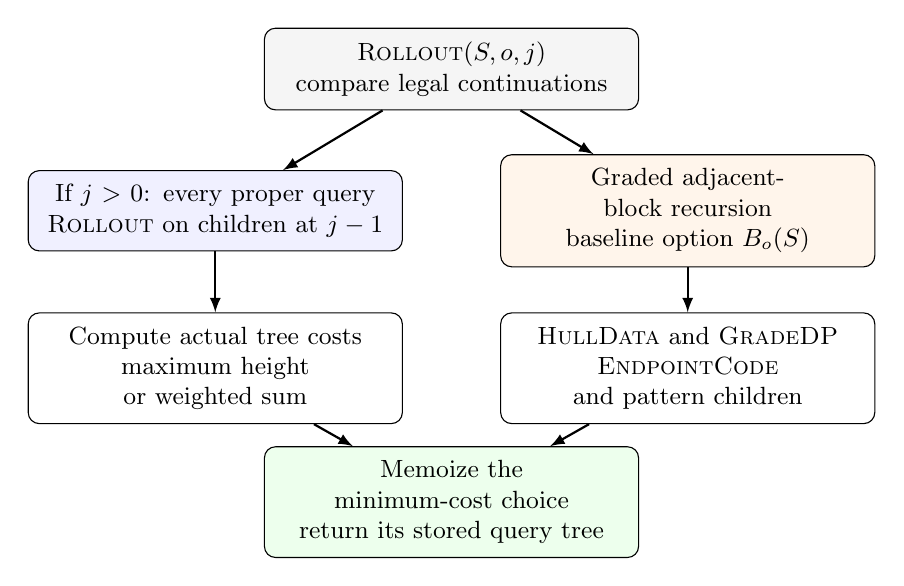
\begin{tikzpicture}[every node/.style={font=\small},
  box/.style={draw,rounded corners,align=center,inner sep=5pt,text width=4.4cm},
  arr/.style={-latex,thick}]
  \node[box,fill=gray!8] (rollout) at (0,0)
    {\Rollout$(S,o,j)$\\compare legal continuations};
  \node[box,fill=blue!6] (split) at (-3,-1.8)
    {If $j>0$: every proper query\\\Rollout\ on children at $j-1$};
  \node[box,fill=orange!8] (baseline) at (3,-1.8)
    {Graded adjacent-block recursion\\baseline option $B_o(S)$};
  \node[box] (grade) at (3,-3.8)
    {\HullData\ and \GradeDP\\\EndpointCode\ and pattern children};
  \node[box] (evaluate) at (-3,-3.8)
    {Compute actual tree costs\\maximum height or weighted sum};
  \node[box,fill=green!7] (best) at (0,-5.5)
    {Memoize the minimum-cost choice\\return its stored query tree};
  \draw[arr] (rollout) -- (split);
  \draw[arr] (rollout) -- (baseline);
  \draw[arr] (baseline) -- (grade);
  \draw[arr] (split) -- (evaluate);
  \draw[arr] (grade) -- (best);
  \draw[arr] (evaluate) -- (best);
\end{tikzpicture}
\caption{Exact lookahead wrapped around the quasipolynomial baseline.
The arrows denote calls and the returned trees or costs. The baseline
completes any branch that reaches its stopping depth. Thus the
logarithmic cap on $j$ bounds the number of search transcripts while
each returned tree still completes identification. The proof compares
this finite search with an optimal tree; the algorithm evaluates only
trees it has constructed.}
\label{fig:qp-procedure-flow}
\end{figure}


\begin{proofstrategy}
\begin{enumerate}
\item Retain several cumulative budgets together. Exact feasibility
      requires nested prefixes, so the graded DP stores their
      compatibility explicitly.
\item Map an optimal witness path to adjacent hull blocks. A query
      already removed by restriction pays for its block delay; a
      count or entropy potential pays for endpoint recovery.
\item Compare lookahead with the first levels of an optimal tree.
      Each paid prefix query replaces a query previously charged at
      factor $a$, which absorbs the continuation penalty.
\end{enumerate}
\end{proofstrategy}

\begin{theorem}\label{thm:qp-two-plus-epsilon}
For every fixed $\varepsilon>0$, maximum depth and
arbitrary-prior expected depth have supplied-query quasipolynomial
$(2+\varepsilon)$ approximations. For $0<\varepsilon\le1$, their time is
\[
(mn)^{O(\varepsilon^{-1}\log n)}
\]
times a polynomial in the
input bit length.
\end{theorem}
\begin{proof}
Use the continuations of Proposition~\ref{prop:qp-baselines} with
$a=2+\varepsilon$. Their penalties on any restricted state are at
most $3\log_2n$ and $4w(S')\ln n$, respectively: $|S'|\le n$
bounds the count potential, and entropy on $|S'|$ hypotheses is at
most $\ln|S'|$ per unit mass. Proposition~\ref{lem:lookahead-completion}
therefore removes both penalties after $O(\log n)$ levels. Concretely, the
final calibration permits
\[
 q_n=\lceil\log_2n\rceil,\qquad
 k=\min\{n-1,\lceil3q_n/(1+\varepsilon)\rceil\}.
\]
When the cap is $n-1$, every proper identifying tree is available,
so the result is exact. Otherwise the lookahead guarantee applies.
At depth $i\le k$, there are at most $2^i$ answer transcripts, and
each transcript is generated by at most $m^i$ choices of supplied
queries along its path. Summing these bounds over $i\le k$ gives
$(2m)^{O(k)}$ lookahead states. Multiplying by the graded-continuation
cost preserves the stated time. For
$\varepsilon>1$, use the construction with $\varepsilon=1$.
\end{proof}

\subsection{Proofs of the supporting propositions}

\subsubsection{Graded schedules retain compatible prefixes}

Each grade prefix has two obligations: stay within its rank budget and
hit every interval whose deadline it represents. Counts enforce the
first; the last selected position suffices to check the second.

\begin{claim}[Counts and last positions decide every interval deadline]
\label{clm:qp-prefix-state}
For each grade prefix $j$, store its selected count $c_j$ and last
selected position $p_j$. When a demand $[l,q]$ ends, it has been
hit within that grade exactly when $p_j\ge l$.
\end{claim}
\begin{proof}
Scan the candidates in spatial order. Selecting position $q$ at
grade $i$ increments $c_j$ and replaces $p_j$ by $q$ for every
$j\ge i$; skipping changes neither. These are exactly the cumulative
counts and last positions. No selected position exceeds the scanned
endpoint $q$, so $p_j\ge l$ is equivalent to a hit in $[l,q]$.
Reject any count exceeding its budget. Sorting the selected
candidates by grade therefore meets every deadline.

Conversely, write the cumulative budgets as $b_j$ and take any
feasible comparison ordering. Drop candidates whose ranks exceed
the last budget; no required deadline hit is lost. Assign each
remaining candidate $v$ the grade
\[
 \operatorname{grade}(v)
   =\min\{j:\operatorname{rank}(v)\le b_j\}.
\]
The candidates with grade at most $j$ are exactly those with
original rank at most $b_j$, so their count is at most $b_j$.
Every demand with deadline $j$ has one such candidate in its
interval. At its right endpoint the last selected position of
that prefix is therefore at least its left endpoint. Thus all
count and hit checks pass, proving the converse. The recurrence
is exact, with at most
$(M+1)^r(B+1)^r$ states and $r+1$ transitions per position.
For circular demands, force the first candidate, delete its hit
demands and cut there. Its absolute rank consumes one unit of
\emph{every} cumulative capacity, including the total-count cap.
\end{proof}

Independent prefix coverage would be insufficient. For example,
$[1,2]$ and $[2,3]$ can both be hit by rank one, while
$\{1\}$ and $\{3\}$ can both be hit by rank two. The first
requirement forces candidate 2 first, leaving too few ranks for the
second. The DP stores exactly this compatibility information.

Exact deadline feasibility must now become an approximation for delay.
Charging the first qualifying grade bounds each positive delay, while
the final selected count also prices the complete negative route.

\begin{claim}[Rounded delays bound the joint objective]
\label{clm:qp-rounded-delay}
Charging a demand at its earliest selected grade gives a
$\lambda$ approximation for $F$, including zero-pattern waiting.
\end{claim}
\begin{proof}
Let $d_0=0$ and let the positive $d_j$ be the distinct
$\lfloor\lambda^j\rfloor$ up to a level covering $n$. Grade $j$
has capacity $d_j+1$. At the right endpoint of demand $I$, charge
$2w(I)d_j$ for the least $j$ whose last selected position lies in
$I$. Its actual first-cover delay is at most $d_j$. Keep the least
accumulated charge for each state, and add $2p_0c_{\rm last}$ at
completion.

For a comparison order, rank one uses grade zero. At rank $t\ge2$,
the first positive level at least $t-1$ is smaller than
$\lambda(t-1)$: the preceding unrounded power is less than the
integer $t-1$. Duplicate-floor plateaus do not change this argument.
These assigned grades respect every cumulative capacity, so
Claim~\ref{clm:qp-prefix-state} makes this graded comparison feasible.
For each positive delay, its rounded charge is at most $\lambda$
times its original charge; the final selected count, and therefore
the zero waiting charge, is unchanged. Since that waiting charge is
nonnegative and $\lambda\ge1$, the minimum surrogate is consequently
at most $\lambda F$. Conversely, the actual delay of each returned
demand is at most its charged grade level, so its actual objective
is no larger than the minimized surrogate.
An optimum uses at most the number of demands, after unproductive
candidates are removed. For a circular order the forced first
candidate has zero delay, all capacities decrease by one, and the
final waiting charge is $2p_0(1+c_{\rm last})$.
\end{proof}

\begin{algorithm}[H]
\caption{\GradeDP: cumulative-grade interval feasibility or weighted delay}
\label{alg:grade-dp}
\KwIn{Ordinary intervals; $r$ capacities $b_0<\cdots<b_{r-1}$;
feasibility deadlines, or weights, delay levels $d_j=b_j-1$,
and zero-pattern mass $p_0$.}
\KwOut{A feasible graded selection, or a minimum surrogate-delay selection.}
Initialize the state $(c_0,\ldots,c_{r-1};s_0,\ldots,s_{r-1})$ to all zeros,
with cost zero; all other states are unreachable\;
\For{$q=1,\ldots,M$}{
  From each reachable state, try skipping $q$ or selecting it at grade $i$\;
  A grade-$i$ selection increments $c_j$ and sets $s_j=q$ for all $j\ge i$\;
  Reject any transition with $c_j>b_j$\;
  \ForEach{interval $I=[l,q]$ ending here}{
    \eIf{mode is feasibility}{
      Reject if $s_j<l$ for its deadline grade $j$\;
    }{
      Find the least $j$ with $s_j\ge l$; reject if none\;
      Add $2w(I)d_j$ to this transition's cost\;
    }
  }
  Keep one feasible witness, or the minimum cost, for each resulting state\;
}
In weighted mode add $2p_0c_{r-1}$ to each final state's cost\;
Reconstruct a winning selection and order it by grade\;
\KwRet the selection and schedule, or infeasible\;
\end{algorithm}

For circular demands enumerate the forced first candidate, remove
its demands, cut there, and reduce \emph{every} capacity by one.
Residual expected costs still use the original delay levels and add
$2p_0(1+c_{r-1})$ at completion. In maximum-depth mode append a final
grade with the total-count cap if it is not already a capacity.
Section~\ref{sec:quasipolynomial} proves the state invariant and
the $(M+1)^{O(r)}(B+1)^{O(r)}$ bound.


\subsubsection{Restriction pays for a graded pattern stage}

For the expected-depth calculations, use the pattern partition $\Pi$
and abbreviate $\Delta=\Delta_{\mathrm E}(S,\Pi)$,
$I=I(S,\Pi)$, $w=w(S)$, and $b=w-w(A_0)$.
Write $J$ for the state-mass-weighted entropy of the actual discovery
transcript, and $W$ for the expected cost of this stage's queries,
before attaching the recursive child trees.

A block rank must be translated back into real queries. The next claim
combines the two possible discovery exits with endpoint recovery;
the second exit benefits from the cached negative first endpoint.

\begin{claim}[An adjacent block has a uniform endpoint allowance]
\label{clm:qp-block-allowance}
If a class $A$ first meets block $k$, its discovery and endpoint
queries use at most
\begin{equation}\label{eq:qp-block-allowance}
 2(k-1)+z_A+5,\qquad
 z_A=\lfloor\log_2(\delta|S|/|A|)\rfloor
\end{equation}
on each route. For expected depth, the analogous overhead is at most
five times the nonzero-pattern mass, plus the pattern information
remaining after discovery.
\end{claim}
\begin{proof}
At most $2(k-1)$ endpoint queries precede the hitting block. A first
endpoint positive costs one query and has endpoint allowance
$z_A+4$ by Proposition~\ref{lem:endpoint-height}. A second endpoint positive costs two queries but has a
cached negative neighbor, reducing its allowance to $z_A+2$.
Thus the two total allowances are respectively
\[
 2(k-1)+1+(z_A+4)=2(k-1)+z_A+5,
\]
\[
 2(k-1)+2+(z_A+2)=2(k-1)+z_A+4.
\]
Their maximum is the stated common allowance.
A block containing the free origin has one real endpoint and obeys
the first bound. For expected depth, the two endpoint-code overheads
are four on the first exit and two on the pinned second exit.
Together with discovery this gives respectively five and four queries
beyond the block delay and the conditional entropy cost. Summing over
positive exits bounds this overhead by $5b$. If $P$ is the pattern
label and $D_{\rm disc}$ the discovery transcript, the latter is a
function of $P$: at this fixed state every discovery query is a hull
test, and all choices and stopping rules depend only on earlier hull
answers. Hence $H(D_{\rm disc}\mid P)=0$, and the entropy chain rule
of Lemma~\ref{lem:entropy-chain-rule} gives
\[
 wH(P\mid D_{\rm disc})=wH(P)-wH(D_{\rm disc})=I-J.
\]
Thus the remaining entropy invoice is $(I-J)/\ln2$. The second
exit's smaller allowance is precisely the negative-neighbor saving.
\end{proof}

For maximum depth, build all pattern-child codes first. For a trial
height $H$, set
\[
 B_A=\left\lfloor\frac{H-B_W(A)-z_A-5}{2}\right\rfloor.
\]
Reject negative budgets. Round each budget down to a delay level,
use block deadline $\widehat B_A+1$, and cap the total selected
blocks at $\lfloor H/2\rfloor$. Enumerate the first block and apply
\GradeDP. The trial range ends at
$\lceil(a+3)(|S|-1)\rceil$. Low-dimensional hulls use their direct
extreme tests.

The computed deadlines use actual child heights, so their feasibility
requires care with integer rounding. Restriction supplies the needed
rank credit before the deadline is rounded down to a grade.

\begin{claim}[Downward rounding retains every required integer rank]
\label{clm:qp-rounded-rank}
At $H^*=\lfloor aD+\gamma\log_2s\rfloor$, where
$D=\OPT_W(S)$ and $s=|S|$, every comparison class is hit by its
computed deadline, provided
\begin{equation}\label{eq:qp-max-parameters}
 \gamma\log_2(1/(1-\delta))\ge1,\qquad
 \gamma\log_2(1/\delta)\ge5,\qquad \gamma\ge1.
\end{equation}
\end{claim}
\begin{proof}
Write $t=t_A$, $x=\log_2(s/|A|)$ and
$u_\delta=\log_2(1/\delta)$. Proposition~\ref{lem:height-prefix} gives
$\OPT_W(A)\le D-(t-1)$. Set
$R_A=a\OPT_W(A)+\gamma\log_2|A|$.
Induction and the integrality of the constructed child height imply
$B_W(A)\le\lfloor R_A\rfloor$, while $z_A=\lfloor x-u_\delta\rfloor$.
Applying $\lfloor u\rfloor-\lfloor v\rfloor\ge\lfloor u-v\rfloor$
twice gives the following chain. The first step uses the inductive
child bound; the second takes the difference of the parent and child
potentials inside one floor; and the third uses the supporting-prefix
credit before taking the second floor difference:
\[
\begin{aligned}
 H^*-B_W(A)-z_A-5
 &\ge\lfloor aD+\gamma\log_2s\rfloor
             -\lfloor R_A\rfloor-\lfloor x-u_\delta\rfloor-5\\
 &\ge\lfloor a(D-\OPT_W(A))+\gamma x\rfloor
             -\lfloor x-u_\delta\rfloor-5\\
 &\ge\lfloor a(t-1)+(\gamma-1)x+u_\delta\rfloor-5.
\end{aligned}
\]
Because $|A|<\delta s$, we have $x>u_\delta$.
The conditions $\gamma\ge1$ and $\gamma u_\delta\ge5$ therefore give
$(\gamma-1)x+u_\delta\ge5$. Hence the last line is at least
$\lfloor a(t-1)+5\rfloor-5=\lfloor a(t-1)\rfloor$.
Dividing the integer credit by two yields
\[
 B_A\ge\left\lfloor\frac{\lfloor a(t-1)\rfloor}{2}\right\rfloor
       =\lfloor\lambda(t-1)\rfloor.
\]
The equality uses $a=2\lambda$ and
$\lfloor\lfloor v\rfloor/2\rfloor=\lfloor v/2\rfloor$.
For $t=1$, level zero suffices. Otherwise choose the last exponent
$j$ with $\lfloor\lambda^j\rfloor\le B_A$, including duplicate
floors. Maximality implies
$\lambda^{j+1}\ge B_A+1>\lambda(t-1)$, so
dividing by $\lambda>0$ gives $\lambda^j>t-1$.
Since $t-1$ is an integer,
$\widehat B_A=\lfloor\lambda^j\rfloor\ge t-1$.
Rounding a real expression before using
this integer credit would not give that conclusion.

Map the optimal witness path to incident hull edges. Each class is
hit by rank at most $t_A$; append an incident edge for an uncovered
terminal nonzero singleton. The comparison uses at most $D$ blocks
when the zero pattern exists, and at most $D+1$ otherwise. The final
calibration ensures $\gamma\log_2s\ge2$ for $s\ge2$.
Since $a\ge2$ and $D$ is an integer,
\[
 H^*=\lfloor aD+\gamma\log_2s\rfloor\ge2D+2,
 \qquad \lfloor H^*/2\rfloor\ge D+1.
\]
The comparison therefore meets the total cap.
Proposition~\ref{prop:qp-grade-schedule} now supplies a passing trial,
and Claim~\ref{clm:qp-block-allowance} bounds every positive route by $H^*$.
The cap also bounds the full negative route, which uses at most
$2\lfloor H^*/2\rfloor\le H^*$ actual tests.
At a balanced state, each child $A$ has
$|A|\le(1-\delta)s$ and $\OPT_W(A)\le D$ by
Lemma~\ref{lem:restriction}. Substituting these two inequalities into
the inductive child bound gives
\[
 1+B_W(A)
 \le aD+\gamma\log_2s
           +1-\gamma\log_2\frac1{1-\delta}
 \le aD+\gamma\log_2s.
\]
The last inequality is exactly the first condition in
\eqref{eq:qp-max-parameters}. For a low-dimensional hull, at most
two extreme tests identify the pattern. Each nonzero class
satisfies $|A|<\delta s$, giving
\[
 2+B_W(A)\le aD+\gamma\log_2s+2-\gamma u_\delta
             \le aD+\gamma\log_2s.
\]
Here the final step uses $\gamma u_\delta\ge5$, so the count-potential
drop pays for both extreme tests.
The zero route ends at its singleton after at most two tests and
also meets the bound because $D\ge1$ and $a\ge2$.
This proves the maximum-depth continuation bound.
\end{proof}

For expected depth, the same witness comparison is summed with the
original hypothesis weights. Discovery information then pays for the
endpoint allowance, giving a local bound that cancels through recursion.

\begin{claim}[Weighted delay and discovery information bound the expected stage]
\label{clm:qp-expected-stage}
The graded expected-depth stage satisfies
\[
 W\le2\lambda\Delta+5b+(I-J)/\ln2,\qquad
 J\ge b\sigma(\delta).
\]
\end{claim}
\begin{proof}
The witness-edge order hits class $A$ by rank $t_A$. When the zero
class exists, its length is at most the witness-path length. Thus
the restriction-credit proposition gives
\[
\begin{aligned}
 F(Q_{\rm wit})
 &=2\sum_{A\ne A_0}w(A)(\operatorname{first}_{Q_{\rm wit}}(A)-1)
     +2p_0|Q_{\rm wit}|
 \\
 &\le2\sum_{A\ne A_0}w(A)(t_A-1)+2p_0\ell\\
 &\byref{Prop.}{lem:support-prefix}{\le}2\Delta.
\end{aligned}
\]
Without the zero class, an
appended terminal singleton has its index $t_A=\ell+1$ and no
waiting term, so the same positive-delay inequality applies.
Claim~\ref{clm:qp-rounded-delay} gives $F(Q_{\rm alg})\le\lambda F(Q_{\rm wit})
\le2\lambda\Delta$.

Adding the allowance of Claim~\ref{clm:qp-block-allowance} yields the
first asserted stage inequality. To bound its information credit, the actual discovery transcript's
positive cells each lie in one vertex cap, even though a comparison
block can meet two caps. Claim~\ref{lem:capped-discovery-entropy} therefore gives
$J\ge b\sigma(\delta)$. Apply Proposition~\ref{lem:stage-conversion} with
$A=2\lambda$ and $B=5$. To see the absorption explicitly,
$ch(\delta)\ge1$ and $h(\delta)\le\ln2$ imply $c\ge1/\ln2$.
Since $0\le J\le I$,
\[
 cI-\frac{I-J}{\ln2}
 =cJ+\left(c-\frac1{\ln2}\right)(I-J)
 \ge cJ\ge cb\sigma(\delta)\ge5b.
\]
In this chain, the first inequality discards the nonnegative term
$(c-1/\ln2)(I-J)$, the second uses the capped-discovery entropy
bound, and the last uses $c\sigma(\delta)\ge5$. Consequently
$W\le a\Delta+cI$.
At a mass-balanced split with relative child mass
$v\in[\delta,1-\delta]$, the query costs $w$ and
$I=wh(v)\ge wh(\delta)$. Thus $cI\ge w$; the nonnegative
restriction decrement permits $w\le a\Delta+cI$ there as well.
Proposition~\ref{prop:potential-cancellation} now adds these local
inequalities over the recursion and cancels every nonroot
optimal-cost and entropy term, giving
$B_E(S)\le a\OPT_E(S)+c\mathcal E(S)$.
The final calibration permits $c=4$.
For a hull of dimension at most one, direct extreme testing costs at
most $2w$. If $p_0>0$, its nonempty zero witness path gives
$\Delta\ge p_0$, so $2w\le2\lambda\Delta+5b$.
Indeed $2w=2p_0+2b\le2\lambda p_0+5b
\le2\lambda\Delta+5b$, since $\lambda\ge1$.
If $p_0=0$, $2w=2b\le5b$. Thus the same stage bound covers the
degenerate branch without invoking the graded DP.
\end{proof}

\begin{algorithm}[H]
\caption{Internal graded continuation for the quasipolynomial algorithm}
\label{alg:qp-baselines}
\KwIn{State $S$; objective $o$; rational $\lambda>1$; fixed balance threshold $1/4$.}
\KwOut{The baseline tree of Section~\ref{sec:quasipolynomial}.}
Stop at a singleton; at a balanced state query a balanced line and recurse\;
At a flat state compute $\HullData(S)$ and use full-hull edges as blocks\;
Handle a hull of dimension at most one by its direct extreme tests\;
\eIf{$o=\mathrm W$}{
  Build the pattern children once and record their heights $C_W(A)$\;
  \For{trial heights $H$ in increasing order}{
    Compute $B_A=\lfloor(H-C_W(A)-z_A-5)/2\rfloor$; reject negative budgets\;
    Round each down to the last level in $\{0\}\cup\{\lfloor\lambda^j\rfloor\}$ not exceeding it\;
    Use deadlines $\widehat B_A+1$ and total cap $\lfloor H/2\rfloor$
    in circular $\GradeDP$; stop at the first feasible trial\;
  }
}{
  Use distinct levels $d_0=0$, $d_j=\lfloor\lambda^j\rfloor$ through a level covering $n$\;
  Minimize the circular weighted-delay surrogate with capacities $d_j+1$
  by $\GradeDP$ and zero-pattern mass $w(A_0)$\;
}
Execute the selected blocks, use pointwise endpoint codes for $\mathrm W$
or expected endpoint codes for $\mathrm E$, and attach recursive pattern children\;
Identify the zero singleton after the negative cover if present; omit it otherwise\;
\KwRet the contracted tree\;
\end{algorithm}

The maximum-depth trial range is
$1\le H\le\lceil(2\lambda+3)(|S|-1)\rceil$.
The baseline selects its trial from these explicit tests, while the
optimum appears in the comparison argument.


There are $O(\varepsilon^{-1}\log n)$ grades, with polynomially many
counts and spatial positions. To compute $z_A$, compare $2^z|A|$
with $\delta|S|$ and choose the largest admissible integer $z$;
this locates the grade directly, without evaluating a logarithm.
All objectives
are rational sums of actual costs. Proper disjoint-child recursion
has at most $n-1$ stages. This proves the time and legality parts of
Proposition~\ref{prop:qp-baselines}.

\subsubsection{Paid prefix queries absorb continuation penalties}

To analyze lookahead, compare with a prefix of an optimal tree. On
every unfinished maximum-depth route, the prefix has already consumed
exactly the queries that create the saving against factor~$a$.

\begin{claim}[The maximum-depth penalty is paid on every frontier path]
\label{clm:lookahead-height-payment}
An optimal height-$D$ tree, truncated at depth $k$, has continuation
height at most $D-k$ at each surviving frontier state.
\end{claim}
\begin{proof}
If $D<k$, the whole optimal tree is a lookahead candidate. Otherwise
each surviving frontier state has optimal height at most $D-k$:
the original optimal subtree is a feasible tree of that height.
The assumed continuation bound therefore completes its path at height
at most
\[
 k+a(D-k)+L_W=aD-(a-1)k+L_W\le aD.
\]
The equality isolates the saving of $a-1$ per paid prefix query, and
the inequality uses $(a-1)k\ge L_W$. Earlier leaves are already
within height $D$. Exact lookahead can only improve this candidate.
\end{proof}

The expected-depth comparison needs no common leaf depth. Only the
mass still unfinished matters: each such hypothesis has paid all
prefix queries, so their total payment absorbs its continuation penalty.

\begin{claim}[Expected prefix cost pays for every surviving frontier mass]
\label{clm:lookahead-expected-payment}
Let $P$ be an optimal tree's expected cost through depth $k$, and
$M_k$ the mass still requiring continuation there. Then $P\ge kM_k$.
\end{claim}
\begin{proof}
Every surviving hypothesis has paid for all $k$ prefix queries.
If $R$ is the sum of the optimal continuation costs, then
$P+R=\OPT_E(S)$ by partitioning the optimal tree's queries at depth
$k$. At each frontier state its optimal restricted cost is no larger
than that of the original subtree, by Lemma~\ref{lem:restriction}.
Thus completing the frontier with the baseline costs
at most
\[
 P+aR+L_EM_k
 =a\OPT_E(S)-(a-1)P+L_EM_k
 \overset{P\ge kM_k}{\le}
 a\OPT_E(S)+[L_E-(a-1)k]M_k.
\]
This is at most $a\OPT_E(S)$ under the stated condition. It assumes
neither a bound on the optimal tree's height nor a lower bound on
its prior masses. These two claims prove the lookahead proposition.
\end{proof}

\subsection{A simple calibration; no optimization is needed}

\begin{parameterchoice}
Fix the balance threshold at $\delta=1/4$, the count coefficient at
$\gamma=3$, and the entropy coefficient at $c=4$. These values
affect only the continuation penalty and lookahead length, which
disappear from the final ratio. Thus no table of optimized constants
is needed for this scheme.
\end{parameterchoice}

Indeed, $(4/3)^3>2$ and $3\log_2 4=6>5$ verify
\eqref{eq:qp-max-parameters}. Here $\sigma(1/4)=\ln4$ and
$h(1/4)\ge\tfrac12\ln2$. The elementary bounds
$2/3\le\ln2<3/4$ give $4h(1/4)>1$ and
$4\sigma(1/4)>5$. The lower bound follows from the first term of
the logarithm series in \eqref{eq:rational-log-bounds}; the upper
bound is the strict trapezoidal bound for $\int_1^2 dx/x$.
Finally $4\ln n<3\log_2 n$, so the single rational lookahead
cap in the theorem covers both objectives. For singleton inputs,
all procedures return the zero-query leaf.

\section{Polynomial maximum depth with rank-subset scheduling}
\label{sec:polynomial-slots}

The algorithm combines exact scheduling inside a logarithmic rank cap
with the priority fallback of Section~\ref{sec:worst}. It constructs
one code for each pattern child and compares scheduling alternatives
against those codes' actual heights. In the proof, an optimal tree
certifies that at least one trial is feasible.

\subsection{The algorithm and its guarantee}

Use the count threshold $\delta$ and potential coefficient $\gamma$
of \eqref{eq:worst-parameter-conditions}. For the original input size
$n$, fix once
\begin{equation}\label{eq:global-slot-cap}
 q=\lceil\log_2n\rceil,\qquad
 R=\left\lfloor\frac{\gamma q}{\gamma-1}\right\rfloor,
 \qquad L=R+1.
\end{equation}
We fix the cap $L$ from the original size $n$ and pass it unchanged to
every recursive child; consequently, the rank-state bound stays uniform
throughout the tree. When a state contains only one hypothesis, its
identity is already known and recursion stops. At every larger state,
we first use a supplied count-balanced query whenever one is available.
Its two answer classes become the next recursive states, each with the
same cap $L$. Once no count-balanced query remains, the state is flat,
and the algorithm proceeds to the scheduling step below.

At a flat state $S$, construct every full hull-pattern child once and
record its actual height $h_A=C_W(A)$. Then try increasing integer
heights $H$ through $\lfloor(3+\gamma)(|S|-1)\rfloor$; because the
children stay fixed, each trial reuses their codes and the first passing
trial gives the smallest certified height. Compare the priority
fallback with exact adjacent-block scheduling. For the latter,
candidates are edges of the full normalized hull, with the origin kept
as a free negative marker. Each positive vertex arc therefore becomes
a circular interval of edge blocks.
Write
\[
 z_A=\lfloor\log_2(\delta |S|/|A|)\rfloor,\qquad
 B_A=\left\lfloor\frac{H-h_A-z_A-5}{2}\right\rfloor.
\]
Proposition~\ref{lem:endpoint-height} bounds the endpoint continuation
by $z_A+4$ queries after the first positive answer; the shared allowance
$z_A+5$ includes the first positive query and also covers a pinned exit.
Thus, after reserving the child height and endpoint allowance, at most
$B_A$ full blocks can precede the hit block, since each uses at most two
queries. This gives deadline $B_A+1$. The total cap
$\lfloor H/2\rfloor$ follows for the same reason: every block costs at
most two queries.
Reject negative budgets; otherwise assign block deadline $B_A+1$ and
use the total cap
\begin{equation}\label{eq:hybrid-total-cap}
 \min\{L,\lfloor H/2\rfloor\}.
\end{equation}
The scheduler receives these integer deadlines directly, so its
feasibility checks match the route-height bounds. An optional exact
whole-exit decoder, proved safe below, may be included in the same
trial. Return a passing alternative at the least height, attach its
endpoint decoders and stored child codes, and contract constant
queries. If the hull has dimension at most one, its two real extreme
tests already determine every pattern, so query them directly.

\begin{algorithm}[H]
\caption{\HybridTree: general polynomial maximum depth}
\label{alg:hybrid-tree}
\KwIn{State $S$, original size $n$, fixed global cap
$L=R+1$, where $q=\lceil\log_2 n\rceil$ and $R=\lfloor\gamma q/(\gamma-1)\rfloor$,
and the count parameters calibrated in Section~\ref{sec:worst-calibration}.}
\KwOut{A tree satisfying Theorem~\ref{thm:poly-slot-worst}.}
Stop at a singleton; at a count-balanced state query a balanced line and recurse\;
Compute $\HullData(S)$ and build each child's hybrid code once\;
Handle a low-dimensional hull directly; otherwise record child heights $h_A$\;
\For{$H=1,\ldots,\lfloor(3+\gamma)(|S|-1)\rfloor$}{
  Try $\PriorityTrial$ with these stored children\;
  Set $z_A=\lfloor\log_2(\delta|S|/|A|)\rfloor$ and
  $B_A=\lfloor(H-h_A-z_A-5)/2\rfloor$\;
  \If{all $B_A\ge0$}{
    Try circular $\SlotDP$ on full-hull-edge demands with deadlines $B_A+1$
    and slot cap $\min\{L,\lfloor H/2\rfloor\}$\;
  }
  Optionally try whole-exit $\SlotDP$ using actual endpoint-continuation
  heights and the same total cap; test feasibility with these heights\;
  \If{any alternative passes}{
    Attach its endpoint decoders and the stored child trees\;
    Terminate the negative cover at $A_0$ when present; omit that leaf otherwise\;
    \KwRet a passing tree, contracting constant queries\;
  }
}
\end{algorithm}

The global cap is inherited unchanged by every child. The priority
fallback proves that a trial always passes; the algorithm never tests
the unknown condition $\OPT_W(S)\le R$.

\begin{figure}[htbp]
\centering
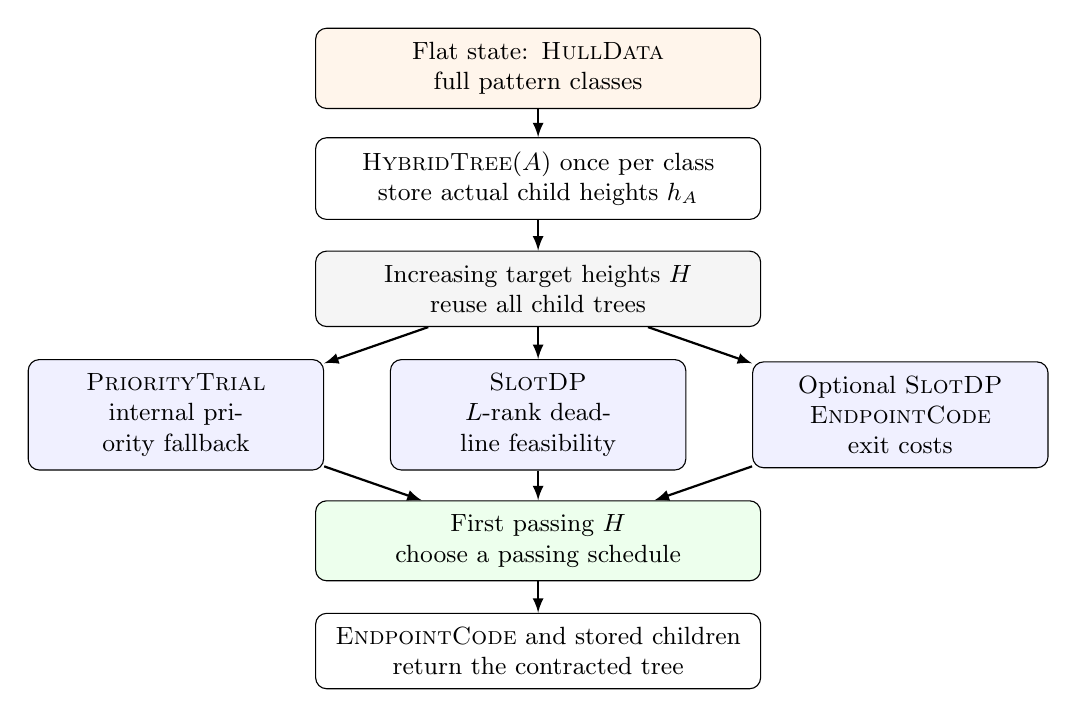
\begin{tikzpicture}[every node/.style={font=\small},
  box/.style={draw,rounded corners,align=center,inner sep=5pt,text width=3.4cm},
  wide/.style={box,text width=5.3cm},arr/.style={-latex,thick}]
  \node[wide,fill=orange!8] (hull) at (0,0)
    {Flat state: \HullData\\full pattern classes};
  \node[wide] (children) at (0,-1.4)
    {\HybridTree$(A)$ once per class\\store actual child heights $h_A$};
  \node[wide,fill=gray!8] (trial) at (0,-2.8)
    {Increasing target heights $H$\\reuse all child trees};
  \node[box,fill=blue!6] (priority) at (-4.6,-4.4)
    {\PriorityTrial\\internal priority fallback};
  \node[box,fill=blue!6] (slots) at (0,-4.4)
    {\SlotDP\\$L$-rank deadline feasibility};
  \node[box,fill=blue!6] (whole) at (4.6,-4.4)
    {Optional \SlotDP\\\EndpointCode\ exit costs};
  \node[wide,fill=green!7] (pass) at (0,-6)
    {First passing $H$\\choose a passing schedule};
  \node[wide] (attach) at (0,-7.4)
    {\EndpointCode\ and stored children\\return the contracted tree};
  \draw[arr] (hull) -- (children);
  \draw[arr] (children) -- (trial);
  \draw[arr] (trial) -- (priority);
  \draw[arr] (trial) -- (slots);
  \draw[arr] (trial) -- (whole);
  \draw[arr] (priority) -- (pass);
  \draw[arr] (slots) -- (pass);
  \draw[arr] (whole) -- (pass);
  \draw[arr] (pass) -- (attach);
\end{tikzpicture}
\caption{At a flat state, the algorithm first computes the hull and
children, then tests increasing target heights using three schedule
checks. The arrows carry the geometry, child heights, and candidate
schedules needed by those checks. The logarithmic cap $L$ is fixed at
the original root. The priority fallback guarantees a passing trial
by the stated height bound; the exact and whole-exit checks can certify
an earlier trial, and the algorithm selects the first trial accepted
by its explicit checks.}
\label{fig:hybrid-procedure-flow}
\end{figure}



\begin{theorem}[General polynomial maximum-depth approximation]
\label{thm:poly-slot-worst}
For separating supplied binary unit-cost planar line queries,
Algorithm~\ref{alg:hybrid-tree} runs in deterministic polynomial time
and returns a tree satisfying
\[
 \boxed{C_W(\HH)\le(2+\gamma)\OPT_W(\HH)<4.464966\,\OPT_W(\HH)}
\]
with the calibrated parameters of Section~\ref{sec:worst-calibration}.
A singleton has cost zero, and every query is a supplied line.
\end{theorem}

\begin{proofstrategy}
\begin{enumerate}
\item Solve interval deadlines exactly by partitioning a small set
of global query ranks (the positions assigned in the full schedule)
between spatial left and right regions.
\item Prove two recursive bounds simultaneously: the priority fallback
works for every optimum; exact scheduling improves it when the optimum
fits the global cap.
\item At the root, a small optimum uses the stronger bound. A large
optimum absorbs the fallback's count potential. Calibrate the two
count-credit inequalities only after these structural arguments.
\end{enumerate}
\end{proofstrategy}

Spatial left and right regions may be queried in an interleaved order.
The exact scheduler assigns each region a subset of global query ranks;
these positions preserve its deadlines while allowing the two searches
to interleave.

\begin{proposition}[Exact rank-subset scheduler]
\label{lem:rank-subset-scheduling}
For $N$ interval demands on $M$ ordered candidates, with integer
first-hit deadlines and at most $L$ distinct selected candidates,
feasibility and a schedule can be found in
$O(M^3 3^L+NM^2)$ time with $O(M^2 2^L)$ states.
Circular intervals add a factor $M$ by enumerating the first candidate.
\end{proposition}

The exact scheduler's short global cap makes its stronger bound
available on small-optimum states, while the priority fallback covers
the remaining states. Proving both bounds together lets the recursion
use the strongest child estimate whose threshold survives restriction.

\begin{proposition}[Two simultaneous recursive guarantees]
\label{prop:slot-invariants}
At every recursive state $S$, with $s=|S|$ and $D=\OPT_W(S)$,
\begin{align}
 C_W(S)&\le3D+\Phi(s),\label{eq:slot-universal-invariant}\\
 D\le R\quad\Longrightarrow\quad
 C_W(S)&\le2D+\Phi(s).\label{eq:slot-restricted-invariant}
\end{align}
The threshold $R$ is global, so restriction preserves the second
invariant's inductive hypothesis in every child.
\end{proposition}

A feasible abstract schedule must still account for actual endpoint
queries, stored child continuations, and the negative route. The next
statement connects those certificates to a finite legal construction.

\begin{proposition}[Executable trials and polynomial reconstruction]
\label{prop:slot-construction}
Every accepted trial has complete height at most $H$, including its
zero route when present. A passing trial is reached within the stated
range; geometry, scheduling, endpoint decoding, and reconstruction
have polynomial bit complexity. The optional whole-exit alternative
preserves both guarantees in Proposition~\ref{prop:slot-invariants}.
\end{proposition}

\begin{proof}[Proof of Theorem~\ref{thm:poly-slot-worst}]
At the root, if $D\le R$, \eqref{eq:slot-restricted-invariant} gives
$C_W\le2D+\Phi(n)\le2D+\gamma\log_2n\le(2+\gamma)D$.
The middle step removes the floor from $\Phi(n)$, while
Claim~\ref{clm:restriction-3} gives $D\ge\log_2n$; together these
facts bound the logarithmic potential by $\gamma D$.
If $D>R$, integrality gives
$D\ge R+1>\gamma q/(\gamma-1)$. Since $\log_2n\le q$,
this implies $\gamma\log_2n/D<\gamma-1$.
Substituting this bound into \eqref{eq:slot-universal-invariant} therefore gives
\[
 \frac{C_W}{D}\le3+\frac{\gamma\log_2n}{D}
 <3+(\gamma-1)=2+\gamma.
\]
Proposition~\ref{prop:slot-construction} supplies the legal
polynomial construction, and the calibration below gives its numerical
factor. Trial acceptance is determined by the constructed code; the
proof uses $D$ to show that one of the checked trials meets the bound.
\end{proof}

\subsection{Technical proofs of the propositions}

\begin{proof}[Proof of Proposition~\ref{lem:rank-subset-scheduling}]
The scheduler's state separates spatial information from temporal
information. A spatial split removes the intervals it hits; absolute
ranks preserve every deadline while allowing the left and right
searches to interleave in any order.


Candidates are $1,\ldots,M$. A demand $[a,b]$ of deadline $d$
must contain a selected candidate assigned a rank at most $d$.
For region $[l,r]$, let $\mathcal I(l,r)$ contain the original
demands wholly inside it. Define $F(l,r,T)$ for an available subset
$T\subseteq[L]$ of absolute ranks; unused ranks are allowed.
The key sufficiency question is which demands can still matter inside
a region. Interval geometry makes ancestor hits recognizable from the
region alone, while the rank subset records its remaining time slots.

\begin{claim}[Contained intervals are exactly the unhit demands]
\label{clm:slot-contained-state}
The spatial region and the absolute rank subset are sufficient state.
\end{claim}
\begin{proof}
Each region is a connected component of the candidate line after
its ancestor separator points have been deleted. An original interval
not contained in one such component must contain a deleted separator:
intervals contain every candidate between their endpoints. It was
therefore hit at an ancestor. Conversely, an interval contained in a
remaining region contains none of those separators and is unhit.
Queries in other remaining regions cannot hit it either. Thus exactly
$\mathcal I(l,r)$ remains relevant in $[l,r]$. The subset $T$ records
when its future candidates may be queried in the global order; two
regions with the same number of queries can have different available
ranks and hence different deadline feasibility.
\end{proof}
Once that state is sufficient, its earliest available rank can be used
for the next separator. Partitioning the later ranks permits every
interleaving of the left and right searches.

\begin{claim}[The earliest available rank gives an exact recurrence]
\label{clm:slot-earliest-rank}
For nonempty $\mathcal I(l,r)$ and $T$, put $t=\min T$.
Reject if a contained deadline is less than $t$; otherwise accept
precisely when some $p\in[l,r]$ and partition
$T\setminus\{t\}=T_L\mathbin{\dot\cup}T_R$ satisfy
\[
 F(l,p-1,T_L)\quad\hbox{and}\quad F(p+1,r,T_R).
\]
\end{claim}
\begin{proof}
By Claim~\ref{clm:slot-contained-state}, it suffices to check the
contained demands. For sufficiency, place $p$ at rank $t$. Every contained demand
containing $p$ is hit at rank $t$, no later than its deadline because
the preliminary test checked every contained deadline. An interval
not containing $p$ is wholly in $[l,p-1]$ or $[p+1,r]$.
The two accepted subproblems give distinct candidates with disjoint
absolute rank sets, so merging their selections by rank preserves
all their deadlines and completes the state.

For necessity, let a feasible state have first selected point $p$
at rank $t'\in T$, and put $t=\min T$. If $t<t'$, then $t$ is
unused: every other selected point has rank greater than $t'$. Assign
$p$ to $t$ and keep all other ranks fixed. If $t=t'$, leave the
schedule unchanged. Thus selected ranks remain distinct, and advancing
the first point cannot delay any first hit.
No contained deadline can be smaller than $t$, since no available
rank would then meet it. Partition the other selected ranks by
whether their candidate lies left or right of $p$, and distribute
unused ranks arbitrarily between the two parts. Each unhit interval
lies wholly on one side, so the corresponding subproblem is feasible.
This gives a partition of all $T\setminus\{t\}$ as required.
When the demand family is empty, the empty selection is feasible; a
nonempty family with $T=\varnothing$ is infeasible.
\end{proof}
The DP may leave rank gaps, which only postpone hits. Compressing
those gaps produces an executable linear schedule; choosing its first
point similarly turns a circular instance into a linear one.

\begin{claim}[Reconstruction and circular cuts preserve feasibility]
The recurrence has the stated time and state bounds.
\end{claim}
\begin{proof}
Sort selected points by their assigned ranks and remove unused slots;
all hits accelerate. Precompute existence and minimum deadline of
contained demands in $O(NM^2)$ time. There are $O(M^2 2^L)$ states,
and for a mask of size $k$ there are at most $2^{k-1}$
partitions after its minimum is removed. The coarser total bound is
\[
 \sum_{T\subseteq[L]}2^{|T|}
 =\sum_{k=0}^L\binom Lk2^k=(1+2)^L=3^L.
\]
The first equality groups masks by cardinality, and the second is
the binomial theorem. Hence all masks contribute a total partition
factor $3^L$. With $O(M^2)$ spatial regions and at most $M$ candidate
roots per region, the transitions take $O(M^3 3^L)$ time, in addition
to the $O(NM^2)$ preprocessing. Removing unused ranks sends every
assigned rank to an earlier or equal schedule position, so no deadline
is missed.

An empty circular demand family accepts immediately. Otherwise
enumerate its first selected point at rank one. Delete the intervals
hit there and cut the candidate circle at that point; every survivor
becomes an ordinary interval. A surviving original deadline at most
one is impossible. For all other survivors subtract one from their
deadline and use $L-1$ remaining slots. Appending the first point
to any accepted linear schedule restores the original deadlines,
and every feasible circular schedule has one of the enumerated first
points. The enumeration adds a factor $M$.
\end{proof}
\end{proof}

Within an interval state, the earliest available rank must be assigned
to one candidate $p$. Choosing $p$ divides the remaining candidates
into left and right intervals, and the unused ranks must split between
those two subproblems. The recursion enumerates these partitions;
memoization reuses each interval-and-rank state.

\begin{algorithm}[H]
\caption{\SlotDP: exact interval deadlines with a rank subset}
\label{alg:slot-dp}
\KwIn{Ordinary interval demands and deadlines; region $[l,r]$;
available absolute ranks $T\subseteq[L]$.}
\KwOut{A feasible rank assignment, or infeasible.}
\If{no original demand is wholly contained in $[l,r]$}{\KwRet the empty assignment\;}
\If{$T=\varnothing$}{\KwRet infeasible\;}
\If{this state is memoized}{\KwRet its stored result\;}
$t\gets\min T$\;
\If{a wholly contained demand has deadline $<t$}{\KwRet infeasible\;}
\ForEach{$p\in[l,r]$ and $T_L\subseteq T\setminus\{t\}$}{
  $T_R\gets T\setminus(T_L\cup\{t\})$\;
  Recurse on $([l,p-1],T_L)$ and $([p+1,r],T_R)$\;
  \If{both assignments are feasible}{
    Memoize their union with $(p,t)$ and \KwRet it\;
  }
}
Memoize and return infeasible\;
\end{algorithm}

After the recursion succeeds, sort the selected candidates by rank and
suppress unused ranks to obtain the schedule. For circular demands,
enumerate the first candidate and cut the circle there; this converts
the remaining demands to intervals, with one subtracted from their
deadlines and the slot cap to account for the forced first rank.
In the optional complete-exit variant, first compute both oriented
decoder costs using Algorithm~\ref{alg:endpoint-code}. Those costs
replace the ordinary deadline precheck by the local height tests of
Section~\ref{sec:polynomial-slots}; the same rank partitions then
handle the remaining scheduling choices.


\begin{proof}[Proof of Proposition~\ref{prop:slot-invariants}]
Induct on $s$, with zero-cost singleton states, proving both bounds
simultaneously. A balanced child $A$ has $\OPT_W(A)\le D$ and
$\Phi(|A|)\le\Phi(s)-1$, by restriction and
Proposition~\ref{lem:worst-floor-credit}. For either coefficient
$c\in\{2,3\}$, its inductive route bound gives
\[
 1+h_A\le1+c\OPT_W(A)+\Phi(|A|)
          \le cD+\Phi(s).
\]
The first inequality is the appropriate inductive hypothesis; in the
second, restriction bounds the optimal child height by $D$ and the
unit potential drop pays for the root query.
When $c=2$, $D\le R$ also gives $\OPT_W(A)\le R$, so the
stronger child hypothesis is available. Thus a balanced query
preserves either bound. The priority alternative
preserves the universal bound by Proposition~\ref{thm:worst}; smaller
actual children only improve its budgets.

For the stronger flat-state bound, assume $D\le R$ and put
$H^*=2D+\Phi(s)$. All children meet the same global threshold, so
their stronger inductive bound is available.
The stronger flat-state proof has three parts: convert child-height
credit into deadlines, fit a comparison cover inside both caps, and
translate its blocks into physical routes. The optimal witness is used
only to establish existence of a passing trial.

\begin{claim}[Actual child heights give feasible comparison deadlines]
\label{clm:slot-child-deadlines}
Every nonzero class satisfies $B_A+1\ge t_A$ at $H^*$.
\end{claim}
\begin{proof}
Proposition~\ref{lem:height-prefix} gives $\OPT_W(A)\le D-(t_A-1)$.
The actual stored height therefore satisfies
$h_A\le2[D-(t_A-1)]+\Phi(|A|)$. Substitution gives
\begin{align*}
 H^*-h_A-z_A-5
 &\ge2(t_A-1)+\Phi(s)-\Phi(|A|)-z_A-5\\
 &\ge2(t_A-1),
\end{align*}
The first inequality substitutes the stronger inductive child bound;
the second uses the nonzero-class count credit of
Proposition~\ref{lem:worst-floor-credit}, namely
$\Phi(s)-\Phi(|A|)\ge z_A+5$. Thus
\begin{equation}\label{eq:slot-deadline-credit}
 H^*-h_A-z_A-5\ge2(t_A-1).
\end{equation}
Dividing by two gives a lower bound by the integer $t_A-1$;
taking a floor consequently preserves it, so $B_A\ge t_A-1\ge0$.
Thus this comparison trial passes the nonnegative-budget check and has
deadline $B_A+1\ge t_A$.
This links an unknown optimal witness to deadlines computed from
actual stored codes.
\end{proof}
The comparison must satisfy each block deadline, the global rank cap,
and the cap on the negative route. A terminal nonzero singleton may
require one appended block, which accounts for the extra slot in the
global cap.

\begin{claim}[The comparison fits both total caps]
\label{clm:slot-total-caps}
Every class meets its deadline in a cover of at most $D+1$ edge blocks.
\end{claim}
\begin{proof}
Map each witness-path query to a full-hull edge containing its
supports. Enlarging a singleton support only accelerates hits; delete
repeated and unproductive blocks. If the path ends at an uncovered
nonzero singleton, append an incident edge at its supporting index
$r+1$, with $r\le D$. If the zero class exists it is the terminal
witness leaf and no append is needed. The comparison has at most $D$
blocks with a zero class and at most $D+1$ otherwise, and it hits
$A$ by rank $t_A$. Since $D\le R$, this fits $L=R+1$.
Also $s\ge2$ gives $\log_2s\ge1$, and $\gamma>2$ gives
$\Phi(s)=\lfloor\gamma\log_2s\rfloor\ge2$. As $D$ is
an integer,
\[
 \left\lfloor\frac{H^*}{2}\right\rfloor
 =\left\lfloor D+\frac{\Phi(s)}2\right\rfloor
 =D+\left\lfloor\frac{\Phi(s)}2\right\rfloor\ge D+1.
\]
Pulling the integer $D$ through the floor gives the second equality,
and $\Phi(s)\ge2$ gives the final inequality.
Thus the comparison fits both the $L$-block rank limit and the cap
$2\lfloor H^*/2\rfloor$ on the all-negative route, even when a
terminal singleton block has been appended.
\end{proof}
An abstract edge block becomes at most two supplied queries. The
second first-positive exit has a cached negative neighbor and a cheaper
decoder; accounting for this asymmetry yields one safe block allowance.

\begin{claim}[A feasible block trial bounds every physical route]
\label{clm:slot-physical-route}
Class $A$ first hit at block $k$ has complete route height at most
\begin{equation}\label{eq:slot-block-allowance}
 2(k-1)+z_A+5+h_A.
\end{equation}
\end{claim}
\begin{proof}
The preceding $k-1$ blocks use at most $2(k-1)$ supplied queries.
If the first endpoint of block $k$ is positive, discovery uses at
most $2k-1$ queries. Proposition~\ref{lem:endpoint-height} then
adds its $z_A+4$ endpoint allowance and the stored height $h_A$, so
the complete route is bounded by
\[
 (2k-1)+(z_A+4)+h_A=2(k-1)+z_A+5+h_A.
\]
If the second endpoint gives the first positive answer, the first
endpoint is a cached negative neighbor. The pinned allowance in
Proposition~\ref{lem:endpoint-height} therefore gives
\[
 2k+(z_A+2)+h_A=2(k-1)+z_A+4+h_A,
\]
which is one query smaller than the stated common allowance.
A block with one real endpoint obeys the first bound; cached answers
and the origin marker cost nothing. Put $X=H^*-h_A-z_A-5$.
Since $B_A=\lfloor X/2\rfloor$ and $k-1\le B_A$,
\[
 2(k-1)+z_A+5+h_A
 \le2\lfloor X/2\rfloor+z_A+5+h_A
 \le X+z_A+5+h_A=H^*.
\]
The last inequality is $2\lfloor X/2\rfloor\le X$.
Thus either positive route fits the trial. The all-negative route has at most
$2\lfloor H^*/2\rfloor\le H^*$ queries and identifies $A_0$ if
present; an absent zero leaf is omitted.
\end{proof}
Claims~\ref{clm:slot-child-deadlines} and~\ref{clm:slot-total-caps}
provide a feasible comparison schedule. Hence
Proposition~\ref{lem:rank-subset-scheduling} finds a passing trial at
$H^*$, and Claim~\ref{clm:slot-physical-route} converts it into the
required route-height bound.
If the hull has dimension at most one, its at most two extreme tests
learn the pattern directly. For a nonzero class the stronger child
bound and Proposition~\ref{lem:worst-floor-credit} give
$2+h_A\le2D+\Phi(s)-z_A-3\le H^*$, since $z_A\ge0$.
The all-negative route also uses at most two tests, and $H^*\ge2$.
The universal calculation is identical with coefficient three.
Both invariants follow by induction.
\end{proof}

\begin{proof}[Proof of Proposition~\ref{prop:slot-construction}]
The local route certificate and \eqref{eq:slot-block-allowance} prove
the accepted-height tests. The universal invariant supplies a passing
integer trial. Indeed $D\le s-1$ follows from a proper identifying
tree, and $\log_2s\le s-1$ for integer $s\ge1$, so
\[
 3D+\Phi(s)
 \le3(s-1)+\lfloor\gamma(s-1)\rfloor
 =\lfloor(3+\gamma)(s-1)\rfloor,
\]
where the equality uses the integrality of $3(s-1)$.
The remaining obligations are running time and reconstruction. The
rank search is exponential only in the cap fixed at the root, while
all recursive stages retain explicit supplied queries and child codes.

\begin{claim}[The global cap makes exact scheduling polynomial]
All arithmetic and the complete reconstructed tree have polynomial size.
\end{claim}
\begin{proof}
For fixed $\gamma$, put $\alpha=\gamma/(\gamma-1)$.
For $n\ge2$, $q=\lceil\log_2n\rceil<\log_2n+1$ and
$L=\lfloor\alpha q\rfloor+1<\alpha\log_2n+\alpha+1$.
For either $b=2$ or $b=3$, exponentiating gives
\[
 b^L<b^{\alpha+1}b^{\alpha\log_2n}
     =b^{\alpha+1}n^{\alpha\log_2b}.
\]
The inequality uses monotonicity of $b^x$ for $b>1$, and the
equality follows from $b^{\log_2n}=n^{\log_2b}$.
The constants are fixed, so both rank-mask costs are polynomial.
The singleton input returns immediately. There are polynomially many
trial heights and first blocks, and at most $n-1$ nonterminal
recursive stages with disjoint child sets. To see this count, the
recursive states form a rooted partition tree whose leaves are
individual hypotheses. Each nonterminal state has at least two
nonempty children: balanced queries split properly, and a flat
nonsingleton state cannot be one class because every nonzero class
has size less than $\delta s$ and the zero class has size at most
one. In a rooted tree with $n$ leaves and at least two children at
each internal vertex, counting edges gives at most $n-1$ internal
vertices. The witness LP, hull
incidence, and endpoint codes have polynomial bit complexity.
Every recursive child is smaller: balanced queries split properly,
nonzero patterns have size below $\delta s$, and $A_0$ is a singleton.
Compute $q$ and $z_A$ from their defining power-of-two thresholds, then
set $R=\lfloor\gamma q/(\gamma-1)\rfloor$. Priority weights
have $O(n\log n)$ bits. Contracting constant queries gives a proper
tree with at most $n$ leaves and $n-1$ internal nodes.
\end{proof}
Fixed endpoint allowances make the deadline instance simple, but may
overestimate a particular exit. An exact rectangle decoder can inspect
the realized patterns and their stored continuations. It uses the same
legal endpoint comparisons and therefore can only improve a trial.

\begin{claim}[Exact whole-exit decoding cannot weaken a trial]
The optional alternative is polynomial under the same cap and
accepts every fixed-allowance schedule.
\end{claim}
\begin{proofstrategy}
\begin{enumerate}
\item Use dynamic programming on endpoint-coordinate rectangles, and
      prove by induction on the realized classes that the recurrence
      gives the minimum continuation height.
\item Show that unhit interval demands are exactly those contained in
      the current region. This makes each rectangle decoder independent
      of queries already resolved outside it.
\item Compare the minimizing decoder with the explicit endpoint code
      used by a fixed-allowance schedule; its route bounds imply that the
      same schedule passes the more precise height test.
\item Count the rectangles and threshold transitions, then include the
      rank-subset factor $3^L$.
\end{enumerate}
\end{proofstrategy}
\begin{proof}
After the legal cut, each class has one realized endpoint pair; let
$M$ be the number of hull candidate positions.
For a coordinate rectangle $U$, give a one-class leaf value $h_A$
and compute
\[
 E(U)=\min_{\text{proper supplied coordinate thresholds }\ell}
 \bigl(1+\max\{E(U\cap\ell^-),E(U\cap\ell^+)\}\bigr),
\]
ignoring empty outcomes. For an empty rectangle no decoder is
needed. A rectangle containing only class $A$ has value $h_A$;
otherwise two distinct endpoint pairs differ in some coordinate,
and a legal hull comparison between those coordinate values gives
a proper threshold. Each proper threshold sends its realized pairs
to strictly smaller nonempty sets. Induction on the number of realized pairs
shows exactness: every permissible endpoint tree has such a first
threshold and costs one plus the larger continuation height, while
attaching the two minimizing continuations attains that value.
A rectangle is specified by two boundaries in each coordinate,
giving $O(M^4)$ rectangles, with $O(M)$ thresholds to try in each.
The leaf values include the stored class continuations. A pinned
endpoint is the same recurrence in one coordinate.

At state $([l,r],T)$, Claim~\ref{clm:slot-contained-state} identifies
the unhit demands as precisely the original intervals contained in
$[l,r]$. For candidate block $p$ in either
orientation, compute the whole decoder heights $E_1(l,r,p)$ and
$E_2(l,r,p)$ for its first-positive and second-first-positive cells.
These cells depend only on the region and block: an outside query
cannot hit a contained interval, and a crossing interval was already
hit by an ancestor. At $k=\min T$, replace the fixed-deadline check by
\[
 2(k-1)+1+E_1(l,r,p)\le H,\qquad 2k+E_2(l,r,p)\le H,
\]
omitting empty cells. Keep the rank partitions, circular first-block
enumeration, and negative-route cap. These prefixes conservatively
include cached endpoints and the origin. For a cell containing classes $A$, the explicit endpoint code with
their stored continuations is a feasible rectangle decoder tree. Its
whole height is at most $\max_A(e_A^{(4)}+h_A)$ on a first-positive
cell and at most $\max_A(e_A^{(2)}+h_A)$ on a pinned cell.
Therefore the minimizing values $E_1,E_2$ are no larger than these
bounds. If each fixed-allowance class route passes at block rank $k$,
then respectively
$2(k-1)+1+E_1\le H$ and $2k+E_2\le H$.
Keeping the same candidate schedule and negative-route cap thus
passes the whole-exit trial as well. Precomputation and the rank-subset
transitions are polynomial times $3^L$.
\end{proof}
\end{proof}

\subsection{Parameter calibration}
\label{sec:worst-calibration}

\begin{parameterchoice}
The balanced-query and flat-decoder credits require
\[
 \gamma(\delta)=\max\left\{
 \frac1{\log_2(1/(1-\delta))},\,
 \frac5{\log_2(1/\delta)}\right\}.
\]
The first term decreases with $\delta$, while the second increases,
so their maximum is minimized where they meet. Equating them gives
$\delta=(1-\delta)^5$. Let $\delta_0$ be the
unique root of this equation in $(0,1/3)$, and set
\[
 \gamma_0=\frac1{\log_2(1/(1-\delta_0))}
         =\frac5{\log_2(1/\delta_0)}.
\]
In the algorithm, take $\delta=\delta_0$ and $\gamma=\gamma_0$.
The root is unique because $x-(1-x)^5$ is strictly increasing on this
interval: its first term increases and its second decreases. Its values
at $0$ and $1/3$ are $-1$ and $49/243$, respectively, so it crosses
zero once. Thus
$\gamma_0\log_2(1/(1-\delta_0))=1$ and
$\gamma_0\log_2(1/\delta_0)=5$, so both count-credit conditions hold
at equality. To bound the resulting factor,
put $a=245122333/10^9$ and $b=245122334/10^9$. Exact substitution gives
$a-(1-a)^5<0<b-(1-b)^5$, so $a<\delta_0<b$. The first function in
$\gamma(\delta)$ is decreasing and the second is increasing; hence
\[
 \gamma_0\le\frac1{\log_2(1/(1-a))},\qquad
 \gamma_0\le\frac5{\log_2(1/b)}.
\]
Applying the rational logarithm enclosure
\eqref{eq:rational-log-bounds} with $N=100$ to these endpoint
expressions certifies that both upper bounds are less than
$G=2464966/10^6$. More explicitly, if $U_{100}(2)$ is the upper
endpoint for $\ln2$ in that enclosure, the exact rational comparisons
are
\[
 \frac{L_{100}(1/(1-a))}{U_{100}(2)}>\frac{10^6}{2464966},
 \qquad
 \frac{L_{100}(1/b)}{U_{100}(2)}>\frac{5\cdot10^6}{2464966}.
\]
Each numerator is the lower endpoint for its logarithm, so these
comparisons imply the claimed upper bounds on $\gamma_0$. Also
$\delta_0<b<1/4$, so
$1/(1-\delta_0)<4/3<\sqrt2$ (since $16/9<2$) and therefore
$\gamma_0>2$. Thus
\[
 \boxed{2+\gamma_0<4.464966.}
\]
\end{parameterchoice}

The same calibration gives
$\alpha=\gamma/(\gamma-1)$.
Since $q<\log_2n+1$, the rank-mask contributions obey
\[
 3^L<3^{\alpha+1}n^{\alpha\log_2 3},\qquad
 2^L<2^{\alpha+1}n^\alpha,
\]
Thus each is polynomial in $n$, as required for the scheduling
component. The full algorithm's exponent also includes its other stages.
The ceiling $q=\lceil\log_2 n\rceil$ is found by comparing integer
powers of two with $n$.


\section{Stronger algorithms for small caps}
\label{sec:small-caps}

Consider instances with a distinguished hypothesis $p$ and orient
each supplied query so that its \emph{cap} is the answer side missing
$p$. Let $P$ be the other $N$ hypotheses. These assumptions concern
the supplied queries themselves. At a recursive flat state, the
common external witness serves as an analysis aid, while $p$ remains
the distinguished hypothesis.
The restricted algorithms below clarify which small-cap constructions
can support approximation hardness.

\subsection{Exact maximum depth with bounded caps}

\begin{theorem}\label{thm:bounded-cap-height}
If every cap has size at most a fixed integer $b$, maximum depth is
exactly solvable in polynomial time. A running-time bound is
$m^{b-1}2^{O(b^2)}\operatorname{poly}(n,m,L)$, where $L$ is the
input bit length.
\end{theorem}

\begin{proofstrategy}
\begin{enumerate}
\item A minimum cap cover gives a lower bound $K$ from the
witness spine and a tree of height at most $K+b-1$.
\item Only the last $b-1$ witness queries need to be guessed.
Their caps contain at most $b(b-1)$ points, so guess their residual
state and find the earlier cover exactly.
\item Exact local subset tables verify every suffix exit. A feasible
optimal tree supplies one of these guesses, proving exactness.
\end{enumerate}
\end{proofstrategy}

\subsubsection{Supporting propositions and the algorithm}

Let $K$ be the minimum number of supplied caps covering $P$. For a
target height $D\in[K,K+b-1]$, let $d_0=\max\{0,D-b+1\}$.
A suffix guess consists of at most $D-d_0$ ordered witness queries
and the set $R\subseteq P$ alive immediately before them.

The witness path must eliminate every other hypothesis, while each
positive exit contains only a few hypotheses. Comparing these two
requirements confines the optimum to a short interval.

\begin{proposition}[The optimum lies in a short height interval]
\label{prop:cap-height-range}
A minimum supplied-halfplane cover is computable in polynomial time,
and the optimal height lies in $[K,K+b-1]$.
\end{proposition}

Early exits have enough remaining depth for any proper local code.
The only delicate exits occur near the end of the witness path;
preserving their guessed residual set makes the earlier cover independent.

\begin{proposition}[Each suffix guess is exactly checkable]
\label{prop:cap-height-suffix}
Guess $R$ inside the suffix caps' union. A prefix cover of
$P\setminus R$ using caps disjoint from $R$, followed by the suffix,
gives height at most $D$ if its cover size is at most $d_0$ and every
suffix first-hit group $A_j$ satisfies
$j+h(A_j)\le D-d_0$, where $j$ is its first-hit position within the
suffix and $h$ is exact local identification height.
These conditions are decidable in polynomial time for fixed $b$.
\end{proposition}

Exact checking is useful only if an optimum appears among the guesses.
Cutting an optimal witness path at the prescribed depth provides
precisely the small suffix and residual set being enumerated.

\begin{proposition}[Enumeration is complete and polynomial]
\label{prop:cap-height-complete}
Every height-$D$ tree provides an accepted suffix guess. There are
$O(m^{b-1})$ ordered suffixes and $2^{O(b^2)}$ candidate residual
sets per suffix. For $b=1$, a minimum cover itself is exact.
\end{proposition}

\begin{algorithm}[H]
\caption{Exact maximum depth with a distinguished miss hypothesis and bounded caps}
\label{alg:bounded-caps}
\KwIn{Distinguished hypothesis $p$; other hypotheses $P$; supplied caps of size at most fixed $b$.}
\KwOut{An exact minimum-height supplied-query tree.}
\If{$P=\varnothing$}{\KwRet the zero-query tree\;}
Compute the minimum supplied-halfplane cover size $K$ of $P$\;
\For{$D=K,\ldots,K+b-1$}{
  $d_0\gets\max\{0,D-b+1\}$\;
  \ForEach{ordered supplied-query suffix of length $q\le D-d_0$}{
    \ForEach{$R$ contained in the union of its caps}{
      \If{the suffix does not cover $R$}{\Continue\;}
      Find a minimum cover $Q$ of $P\setminus R$ using only caps disjoint from $R$\;
      \If{$|Q|>d_0$ or the cover is infeasible}{\Continue\;}
      Compute the suffix's first-hit groups $A_j$ on $R\cup\{p\}$\;
      \If{some $j+c_W(\ExactTree(A_j,\mathrm W))>D-d_0$}{\Continue\;}
      Execute $Q$ followed by the suffix on the all-miss spine\;
      Attach exact local supplied-query trees to all positive first-hit groups\;
      \KwRet this tree\;
    }
  }
}
\end{algorithm}

The theorem's height interval means the loop needs only the listed
values of $D$. For each value, the algorithm searches suffixes and
residual sets; since a suffix has at most $b-1$ queries and each cap
contains at most $b$ points, its union contains at most $b(b-1)$
points. An empty suffix therefore permits only $R=\varnothing$. The
prefix step is a minimum supplied-halfplane cover, computed by the
polynomial algorithm cited in Theorem~\ref{thm:bounded-cap-height};
when the instance has the special hull-interval representation, its
dedicated interval oracle performs the same step.


\begin{proof}[Proof of Theorem~\ref{thm:bounded-cap-height}]
For $P=\varnothing$, return the zero-query tree. Otherwise,
Proposition~\ref{prop:cap-height-range} limits the target heights.
Proposition~\ref{prop:cap-height-suffix} proves that every accepted
guess constructs a legal tree, and
Proposition~\ref{prop:cap-height-complete} ensures acceptance at the
optimum. Returning the first accepted height is exact; the stated
enumeration and polynomial cover and local optimizations give the
running time.
\end{proof}

\subsubsection{Technical proofs of the height propositions}

\begin{proof}[Proof of Proposition~\ref{prop:cap-height-range}]
Let $K$ be the minimum number of supplied caps covering $P$.
Minimum planar halfplane cover is exactly solvable in polynomial
time~\cite{harpeledlee2012}. Separability ensures that the cover
exists. The path identifying $p$ in any tree must cover $P$, so
its height is at least $K$. Conversely, query a minimum cover along
the all-miss spine and identify each positive hit group locally.
A hit group has at most $b$ members and therefore admits a proper
identification tree of height at most $b-1$. This gives height at
most $K+b-1$. Only these $b$ target heights need to be tested.

\end{proof}

\begin{proof}[Proof of Proposition~\ref{prop:cap-height-suffix}]
For a target $D\in[K,K+b-1]$, put $d_0=\max\{0,D-b+1\}$.
Guess an ordered suffix of $q\le D-d_0\le b-1$ supplied queries
on the witness spine. Guess also the set $R\subseteq P$ remaining
just before that suffix. Require that the suffix caps cover $R$;
thus $R$ is a subset of their union and has size at most $b(b-1)$.
For each guess, compute a minimum cap cover of $P\setminus R$
using only supplied caps disjoint from $R$, and require size at
most $d_0$. An empty suffix permits $R=\varnothing$.

The suffix must fit on both kinds of path: a positive exit needs
its local code, and the all-miss route must also terminate within
the budget. Checking both prevents a hidden witness-path overrun.

\begin{claim}[Local suffix tests include the witness leaf]
The exact checks verify every positive exit and the full miss route.
\end{claim}
\begin{proof}
Execute the guessed suffix on $R\cup\{p\}$. For each nonempty
first-hit group $A_j$ at position $j$, compute its exact local
identification height $h(A_j)$ by subset Bellman DP on at most
$b$ hypotheses. Require $j+h(A_j)\le D-d_0$ and $q\le D-d_0$.
These tests verify the entire suffix tree, including the witness
leaf. The prefix cover takes at most $d_0$ queries, preserves $R$
on its all-miss route, and its positive exits cost at most $b-1$
additional queries. Thus its exits have height at most
$d_0+b-1=D$ when $d_0>0$; if $d_0=0$, the prefix is empty.
The equality here uses the positive branch of
$d_0=\max\{0,D-b+1\}$; no such equality is needed when the prefix
has length zero.
The suffix starts no later than depth $d_0$, so an accepted guess
constructs a tree of height at most $D$.

\end{proof}
\end{proof}

\begin{proof}[Proof of Proposition~\ref{prop:cap-height-complete}]
For completeness, take an identifying tree of height at most $D$. If its witness
path ends before depth $d_0$, use an empty suffix and $R=\varnothing$;
its witness queries cover $P$ within $d_0$. Otherwise take the
remaining witness queries after depth $d_0$ as the suffix, and the
actual nonwitness state there as $R$. The prefix caps are disjoint
from $R$ and cover $P\setminus R$. The suffix has at most $b-1$
queries and covers $R$; its positive subtrees satisfy the exact
local-height tests. This guess is accepted. There are
$O(m^{b-1})$ suffix descriptions and $2^{O(b^2)}$ candidate subsets
per suffix, and all remaining computations are polynomial for
fixed $b$. For $b=1$, a minimum cover itself is exact.
\end{proof}

\subsection{An EPTAS for weighted singleton and pair caps}

Assume every cap has size one or two, all singleton caps for $P$
are supplied, and the graph $G$ of two-point caps is a disjoint
union of paths and cycles. The latter condition follows for planar
instances with all singleton caps: every nonwitness point is a
convex-hull vertex, and a two-point cap joins consecutive vertices.
Let the positive raw weights be $w_0$ for $p$ and $w_v$ for $v\in P$,
and put $\Omega=w_0+\sum_v w_v$.

For a matching $M$, replace each matched pair by a group of mass
$w_u+w_v$ and leave unmatched vertices as singleton groups. Let
$J(M)$ be the group multiset, $k=N-|M|$, and
$P(M)=\sum_{uv\in M}(w_u+w_v)$. With group masses
$a_1\ge\cdots\ge a_k$, write $C(J)=\sum_j j a_j$. The matching
cost is
\begin{equation}\label{eq:eptas-matching-invoice}
 G(M)=w_0k+C(J(M))+P(M).
\end{equation}

\begin{theorem}\label{thm:pair-eptas}
For this weighted singleton/pair path-and-cycle class, expected
depth has a deterministic $(1+\varepsilon)$ approximation in time
$2^{O(\varepsilon^{-3})}\operatorname{poly}(n,L,\log(1/\varepsilon))$
for $0<\varepsilon\le1$. The polynomial exponent is independent
of $\varepsilon$; this is an EPTAS.
\end{theorem}

\begin{proofstrategy}
\begin{enumerate}
\item Delete one residue class of path and cycle edges. Averaging
finds a near-optimal matching on bounded-size components.
\item Enumerate components containing the heaviest vertices. Their
complement has little mass, so only light components need rounding.
\item Express the exact matching cost as a convex quadratic
program on component configurations. Its fractional optimum
lower-bounds the best integral invoice; the computed feasible solution
has only an additive numerical optimization error.
\item Independent configuration rounding adds only a controlled
variance term. Conditional expectations make it deterministic.
\end{enumerate}
\end{proofstrategy}

\subsubsection{Supporting propositions and the algorithm}

Work with raw weights and put $F^*=\min_MG(M)=\Omega\OPT_E$.
The graph, weights, group counts, and count functions below describe
the instance. The tuning controls are integers $K\ge1$, $H\ge0$ and
an additive accuracy $0<\eta\le1$, chosen only in the final calibration.
Put $B=2K$, the resulting component-size bound. Take the $H$ heaviest
nonwitness vertices, or all of them if fewer than $H$ exist, and let
$\Omega_{\rm tail}$ be the mass of the others.

Before approximating matchings, we need to justify that they describe
the full adaptive problem. The witness spine supplies this link;
the supplied singleton queries realize every resulting matching.

\begin{proposition}[The matching cost formula is exact]
\label{prop:pair-invoice-exact}
Minimizing \eqref{eq:eptas-matching-invoice} is exactly the minimum
raw weighted depth, including arbitrary adaptive trees. Every matching
is executable with supplied singleton and pair queries.
\end{proposition}

Two reductions make the remaining optimization manageable. Edge
deletion bounds component size at a small relative cost, while
fixing heavy components leaves little mass exposed to rounding.

\begin{proposition}[Residue deletion and heavy enumeration]
\label{prop:pair-deletion-heavy}
Deleting edge numbers in one residue modulo $K$ leaves components of
at most $B$ vertices. Some residue has a surviving matching of cost
at most $(1+1/K)F^*$. Moreover,
$\Omega_{\rm tail}\le2F^*/(H+1)$, and all matching choices on components
meeting a heavy vertex can be enumerated in at most $2^{BH}$ trials.
\end{proposition}

For a fixed heavy trial, enumerate the matching configurations $c$ of
each remaining, light component $i$. Let $k_{ic}$ be its group count,
$P_{ic}$ its matched-pair mass, and $z_{ic}(t)$ its number of groups
of mass at least $t$. Let $Z_f(t),k_f,P_f$ be the corresponding totals
of the fixed components. Fractional configuration weights satisfy
$x_{ic}\ge0$ and $\sum_cx_{ic}=1$. Set
$\mu(t)=Z_f(t)+\sum_{ic}x_{ic}z_{ic}(t)$ and minimize
\begin{equation}\label{eq:pair-convex-relaxation}
 Q(x)=w_0\left(k_f+\sum_{ic}x_{ic}k_{ic}\right)
       +P_f+\sum_{ic}x_{ic}P_{ic}
       +\frac12\int_0^\infty(\mu(t)^2+\mu(t))\,dt.
\end{equation}

Group order couples choices made in different components. Counting
groups above each mass threshold captures this coupling in one
quadratic objective, without guessing the final order.

\begin{proposition}[An exact convex quadratic model]
\label{prop:pair-convex-model}
The displayed objective equals the matching cost on integral
configurations. Its minimum over the product of configuration simplices
lower-bounds the best integral invoice. It is a rational convex quadratic program
with $N2^{O(B)}$ variables and $O(N)$ mass breakpoints. A feasible
rational solution within raw additive error $\eta\Omega$ is computable
with polynomial bit complexity and time polynomial in the model size,
$L$, and $\log(1/\eta)$.
\end{proposition}

Rounding combines the component choices into one matching. Only the
light components fluctuate, and their mass bounds the extra cost of
turning the relaxation into a tree.

\begin{proposition}[Deterministic rounding costs only light mass]
\label{prop:pair-rounding}
From a feasible rational $x$, conditional expectations produce a matching of
cost at most $Q(x)+(B/2)\Omega_{\rm tail}$ in polynomial time in the
model size and bit length. If every trial uses a feasible rational $x$
within $\eta\Omega$ of its fractional optimum, the cheapest tree over all
residues and heavy trials has cost at most
\[
 \left(1+\frac1K+\eta+\frac B{H+1}\right)F^*.
\]
\end{proposition}

\begin{algorithm}[H]
\caption{Expected-depth EPTAS for weighted singleton/pair paths and cycles}
\label{alg:pair-eptas}
\KwIn{Distinguished miss hypothesis, supplied singleton tests and pair graph $G$;
positive raw weights; $0<\varepsilon\le1$.}
\KwOut{A deterministic $(1+\varepsilon)$ approximation.}
Use the controls $K,H,\eta$ from
Section~\ref{sec:pair-eptas-calibration}; set $B\gets2K$\;
\If{$n=1$}{\KwRet the zero-query tree\;}
Find the $H$ heaviest nonwitness vertices (or all of them if fewer exist)\;
\For{$r=0,\ldots,K-1$}{
  Delete edges numbered $r$ modulo $K$ on each path or cycle\;
  Enumerate each remaining component's matching configurations\;
  \ForEach{joint configuration on components meeting the heavy vertices}{
    Fix these heavy configurations\;
    Solve the light-component convex program \eqref{eq:pair-convex-relaxation}
    to raw additive accuracy $\eta\Omega$\;
    \ForEach{unfixed light component}{
      Fix a configuration minimizing the conditional expected invoice,
      using rational first and second count moments\;
    }
    Form the matched-pair and singleton groups; sort them by decreasing mass\;
    Query the supplied group tests on the miss spine,
    using one supplied singleton test to identify each pair hit\;
    Retain the resulting tree and its exact expected cost\;
  }
}
\KwRet the cheapest retained tree\;
\end{algorithm}

Deleting one edge residue bounds the component size, and enumerating
the heavy components leaves a light-instance relaxation. The
conditional-expectation step then fixes each remaining component while
preserving the invoice bound, so every retained candidate is an actual
matching and hence yields a legal tree. Propositions
\ref{prop:pair-deletion-heavy}--\ref{prop:pair-rounding} prove the
component bound, heavy enumeration, convex relaxation, and rounding
guarantee. Proposition~\ref{prop:pair-invoice-exact} then converts the
rounded matching into its exact tree cost. The fractional solution
guides the rounding, while the returned tree comes from an actual
matching.


\begin{proof}[Proof of Theorem~\ref{thm:pair-eptas}]
For $n=1$, return the exact zero-query tree. For $n\ge2$, choose
$K,H,\eta$ by Section~\ref{sec:pair-eptas-calibration}.
Proposition~\ref{prop:pair-deletion-heavy} provides a good residue and
an enumerated heavy part of its near-optimal matching.
Propositions~\ref{prop:pair-convex-model} and~\ref{prop:pair-rounding}
return cost at most $(1+\varepsilon)F^*$.
Proposition~\ref{prop:pair-invoice-exact} turns the matching into a
legal supplied-query tree. Divide by $\Omega$ to obtain the stated
expected-depth ratio. The calibration gives $BH=O(\varepsilon^{-3})$;
the other stages have polynomial exponent independent of $\varepsilon$.
\end{proof}

\subsubsection{Technical proofs of the EPTAS propositions}

\begin{proof}[Proof of Proposition~\ref{prop:pair-invoice-exact}]
Follow the witness in an arbitrary proper tree. Its first-hit groups
are disjoint singletons or supplied pairs, so the pair groups form
a matching $M$ and the number of groups is $k=N-|M|$. A supplied pair
query first hitting only one vertex can be replaced here
by that vertex's supplied singleton test. The witness contributes
$w_0k$, group positions contribute $\sum_j j a_j$, and each pair
exit needs exactly one further supplied singleton query, contributing
its full pair mass. This is the displayed invoice before sorting.

For adjacent group masses $a<b$, putting $b$ first reduces their
contribution by
$[ja+(j+1)b]-[jb+(j+1)a]=b-a>0$. Thus nonincreasing order minimizes
the position term, giving $C(J(M))$. Conversely, query any matching's
disjoint pairs and unmatched singletons in that order, and attach
one supplied singleton query at each pair exit. This attains
$w_0k+C(J(M))+P(M)$, proving exactness for arbitrary trees.

\end{proof}

\begin{proof}[Proof of Proposition~\ref{prop:pair-deletion-heavy}]
We first control the cost of simplifying the graph, then control
the mass left for rounding. For graph simplification, compare each
residue with the same optimal matching by splitting its deleted pairs.

\begin{claim}[One residue loses at most a $1/K$ fraction]
\label{clm:pair-residue-loss}
Splitting the removed matched edges leaves a legal near-optimal matching.
\end{claim}
\begin{proof}
Number edges consecutively on each path or cycle. For each common
residue $r\in\{0,\ldots,K-1\}$, delete edges numbered $r$ modulo
$K$. A path component between consecutive deleted edges has at most
$K$ vertices, as do its end components. On a cycle, all components
except possibly the one crossing the numbering cut have the same
bound. The crossing component joins two end portions, each with fewer
than $K$ edges, and has at most $2K=B$ vertices. If a residue deletes
no edge of a cycle, that cycle has fewer than $K$ edges, so is already
smaller than $B$.

Take an optimal matching, with sorted group masses
$a_1,\ldots,a_k$. For a matched pair of weights $a\ge b$ at
position $j$, put $R_j=w_0+\sum_{l>j}a_l$. Its original weighted
depth contribution is $(j+1)(a+b)$, including the local pair query.
After replacing it by two consecutive singleton queries the contribution
is $ja+(j+1)b$, a change of $-a$. Every later group and the
witness are delayed by one query, a change of $R_j$. Thus the
net change is exactly $R_j-a$.

For simultaneous splits, each earlier split delays all points of a
later group by one regardless of whether that group is also split.
The local change $-a$ is likewise independent of the group's shifted
position. The net changes therefore add. Sorting the new singleton
and pair groups can only improve the temporary schedule. Since the
$R_j$ are positive,
\[
 \sum_{j\text{ matched}}R_j
 \le\sum_{j=1}^k R_j
 =kw_0+\sum_{l=1}^k(l-1)a_l
 \le kw_0+C(J)\le F^*.
\]
The first inequality adds the remaining nonnegative $R_j$ terms.
For the equality, group $l$ contributes to exactly $l-1$ earlier
tails. Replacing $l-1$ by $l$ gives the next inequality, and the
last discards the nonnegative pair-continuation term from the exact
invoice of Proposition~\ref{prop:pair-invoice-exact}.
Each matched edge belongs to exactly one residue trial. Averaging
the temporary schedules over the $K$ residues gives cost at most
\[
 F^*+\frac1K\sum_{j\text{ matched}}(R_j-a)
 \le F^*+\frac{F^*}{K}.
\]
This inequality first discards each nonpositive local saving $-a$
and then applies the preceding bound on the summed tails.
At least one trial meets this average bound, and sorting its groups
produces a surviving matching of no larger cost.

\end{proof}
A component can be small in vertex count yet carry a heavy vertex,
raising the rounding cost. Enumerating the heavy part removes this
risk, while the rank lower bound controls the remaining mass.

\begin{claim}[Heavy components leave a low-mass rounding problem]
\label{clm:pair-heavy-tail}
The rank lower bound controls all unfixed vertex mass.
\end{claim}
\begin{proof}
Order individual nonwitness weights as $w_{(1)}\ge\cdots\ge w_{(N)}$.
A first-hit group contains at most two vertices, so at most $2j$
vertices can leave by spine position $j$. Consequently the sorted
list of first-hit positions is componentwise at least
$\lceil1/2\rceil,\ldots,\lceil N/2\rceil$.
Pairing larger weights with smaller positions minimizes their weighted
sum by adjacent exchanges. Ignoring local continuation and witness
costs therefore gives
\[
 F^*\ge\sum_{i=1}^N\lceil i/2\rceil w_{(i)}.
\]
For every $i>H$, $\lceil i/2\rceil\ge(H+1)/2$, hence
\[
 F^*\ge\sum_{i>H}\lceil i/2\rceil w_{(i)}
 \ge\frac{H+1}{2}\sum_{i>H}w_{(i)}
 =\frac{H+1}{2}\Omega_{\rm tail}.
\]
The first inequality drops the nonnegative contributions of the
heaviest $H$ vertices, and the second applies the rank lower bound
uniformly to every remaining index. Thus the tail mass is bounded
without assuming any lower bound on an individual weight.
For each residue, enumerate all matching configurations in components
containing one of the $H$ heaviest vertices. There are at most $H$
such components. A path or cycle on at most $B$ vertices has at most
$B$ edges, so has at most $2^B$ edge subsets and hence at most that
many matching configurations. The joint number of choices is at most
$(2^B)^H=2^{BH}$. This enumeration
is independent of $n$ in its exponent. The remaining components'
total vertex mass is at most $\Omega_{\rm tail}$. If $H\ge N$,
all components are fixed and there is no rounding stage.

\end{proof}
\end{proof}

\begin{proof}[Proof of Proposition~\ref{prop:pair-convex-model}]
For sorted group masses $a_1\ge\cdots\ge a_k$,
the groups above a threshold occupy ranks $1$ through $Z(t)$.
Finite summation and integration therefore give
\[
 C(J)=\sum_{j=1}^k j a_j
     =\int_0^\infty\sum_{j:a_j\ge t}j\,dt
     =\int_0^\infty\frac{Z(t)(Z(t)+1)}2\,dt.
\]
For the first integral, integrate the indicator of $t\le a_j$
over $t\ge0$ and sum over $j$. The second integral then sums the
consecutive ranks $1,\ldots,Z(t)$. Consequently the formula prices
all cross-component ordering effects exactly.
On integral configurations, $\mu(t)=Z(t)$ and the linear
terms are exactly the witness and pair-continuation terms of the
invoice. Allowing fractional configurations enlarges the feasible
set, so its minimum cannot exceed the integral minimum.
The only breakpoints are singleton and available-pair masses, at most
$N+|E(G)|=O(N)$ rational values. Include zero among the ordered
breakpoints $\tau_j$. On each interval between consecutive breakpoints,
$\mu(t)$ is a fixed affine function $\mu_j(x)$, so the integral is
\[
 \frac12\sum_j(\tau_{j+1}-\tau_j)
                 \bigl(\mu_j(x)^2+\mu_j(x)\bigr).
\]
The coefficients are rational and the interval lengths are nonnegative;
thus its quadratic part is a nonnegative sum of squares of affine
functions and is convex. Each component has at most $2^B$ matching
configurations and there are at most $N$ components, giving
$N2^{O(B)}$ variables over a product of simplices. After normalizing by $\Omega$, solve it to additive
accuracy $\eta$ using polynomial-time convex quadratic
optimization~\cite{nestnem1994}. Equivalently the raw error is $\eta\Omega$. The simplex
constraints have rational coefficients and a feasible integral point
obtained by choosing one configuration per component.
For any feasible fractional point, $0\le\mu(t)\le N$ and
$\int\mu(t)\,dt=\sum_vw_v$, since every configuration partitions
its component's vertices. Its witness term is at most $Nw_0$,
its pair-continuation term is at most $\sum_vw_v$, and
\[
 \frac12\int(\mu(t)^2+\mu(t))\,dt
 \le\frac{N+1}{2}\int\mu(t)\,dt
 =\frac{N+1}{2}\sum_vw_v.
\]
Here $\mu(t)^2\le N\mu(t)$ follows pointwise from
$0\le\mu(t)\le N$, and the equality uses the invariant total group
mass across configurations.
Thus $0\le Q(x)\le(N+3)\Omega$, giving a normalized objective
bound $O(n)$. Together with bounded simplices and rational
coefficients of polynomial bit length, the cited convex-QP algorithm
provides the stated feasible rational approximation and bit complexity.

\end{proof}

\begin{proof}[Proof of Proposition~\ref{prop:pair-rounding}]
We separate the rounding analysis from its deterministic implementation.
The fractional objective records the mean counts; independent rounding
changes only their quadratic contribution, which can be charged to
light vertex mass.

\begin{claim}[Only the quadratic count term incurs variance]
\label{clm:pair-rounding-variance}
The expected rounded cost is at most $Q(x)+(B/2)\Omega_{\rm tail}$.
\end{claim}
\begin{proof}
Independently round each light component according to its fractional
configuration distribution, and write
$Z(t)=Z_f(t)+\sum_iX_i(t)$. Then $\mathbb EZ(t)=\mu(t)$.
For each component $0\le X_i(t)\le B$, so
\[
 \operatorname{Var}X_i(t)
 =\mathbb E[X_i(t)^2]-(\mathbb EX_i(t))^2
 \le\mathbb E[X_i(t)^2]\le B\mathbb EX_i(t).
\]
The first inequality removes a nonnegative square; the second uses
$X_i(t)^2\le BX_i(t)$ on $[0,B]$. Hence the variance bound depends
on component size and expected mass, regardless of how many
configurations the component has.
Independence gives
$\mathbb E[Z(t)^2]=\mu(t)^2+\sum_i\operatorname{Var}X_i(t)$.
The witness and pair-continuation terms are linear, so their expectations
are exactly their terms in $Q(x)$. Applying the rank integral from
Proposition~\ref{prop:pair-convex-model} and then the variance bound yields
\begin{align*}
 \mathbb EG(M)
 &=Q(x)+\frac12\int_0^\infty
                 \sum_i\operatorname{Var}X_i(t)\,dt\\
 &\le Q(x)+\frac B2\sum_i
                  \int_0^\infty\mathbb EX_i(t)\,dt.
\end{align*}
For every configuration, the integral of its count function is the
sum of its group masses. These groups partition the component's
vertices, so this sum is its fixed vertex mass, independent of the
configuration. The displayed sum of integrals is therefore the total
light-component mass, at most $\Omega_{\rm tail}$. Hence
\[
 \mathbb EG(M)\le Q(x)+\frac B2\Omega_{\rm tail}
                 \byref{Prop.}{prop:pair-deletion-heavy}{\le} Q(x)+\frac B{H+1}F^*,
\]
using the tail bound proved above.
\end{proof}
An expected-cost bound still needs an individual matching that attains
it. Fixing one component at a time preserves that bound and keeps
all intermediate computations rational and explicit.

\begin{claim}[Exact conditional expectations give a supplied tree]
One component at a time can be fixed without increasing the expected invoice.
\end{claim}
\begin{proof}
Suppose some components have already been fixed. For the next
component, the current conditional expected invoice is the weighted
average of the conditional expected invoices obtained by fixing each
configuration, with weights $x_{ic}$ summing to one. At least one
configuration of positive probability therefore has value no larger
than the current expectation. Choose a minimum such value and repeat.

Compute each value exactly from the fixed counts and the remaining
independent first and second count moments at the same $O(n)$
breakpoints. The identity for $\mathbb E[Z(t)^2]$ remains valid with
the fixed counts incorporated into $Z_f(t)$. All interval lengths,
probabilities, moments, and linear terms are rational, with polynomial
bit length; the number of configurations and breakpoints is the model
size. At the end no randomness remains, so the actual matching cost is
at most the initial expectation. Sorting its final groups yields
a supplied-query tree by Proposition~\ref{prop:pair-invoice-exact}.

\end{proof}
For the good residue, enumeration contains the heavy part of an optimum
surviving matching. The fractional optimum is no greater than that
matching's invoice. In a nontrivial instance every hypothesis has depth at least one,
so $F^*\ge\Omega$. For the good residue and heavy trial, the computed
feasible point thus satisfies
\[
 Q(x)\byref{Prop.}{prop:pair-convex-model}{\le} Q^*+\eta\Omega
       \byref{Prop.}{prop:pair-deletion-heavy}{\le}(1+1/K)F^*+\eta F^*.
\]
Claim~\ref{clm:pair-residue-loss} bounds the surviving comparison
invoice, while $F^*\ge\Omega$ converts the numerical error to a
relative one. Adding Claim~\ref{clm:pair-rounding-variance}, with the
tail estimate of Claim~\ref{clm:pair-heavy-tail}, gives cost at most
\[
 (1+1/K)F^*+\eta F^*+\frac B{H+1}F^*
 =\left(1+\frac1K+\eta+\frac B{H+1}\right)F^*.
\]
The algorithm takes the cheapest trial, so it meets this same bound.
\end{proof}

\subsubsection{Calibration of the EPTAS controls}
\label{sec:pair-eptas-calibration}

\begin{parameterchoice}
For $0<\varepsilon\le1$, choose
\[
 K=\lceil3/\varepsilon\rceil,\qquad B=2K,\qquad
 H=\lceil3B/\varepsilon\rceil,\qquad \eta=\varepsilon/3.
\]
Then $1/K+\eta+B/(H+1)\le\varepsilon$.
Also $B=O(\varepsilon^{-1})$ and $H=O(\varepsilon^{-2})$, so heavy
enumeration costs $2^{O(\varepsilon^{-3})}$. Configuration enumeration,
convex optimization, and conditional expectations keep a polynomial
exponent independent of $\varepsilon$.
\end{parameterchoice}

The ceiling choices give $K\ge3/\varepsilon$ and
$H+1\ge3B/\varepsilon$, hence
$1/K\le\varepsilon/3$ and $B/(H+1)\le\varepsilon/3$.
Together with $\eta=\varepsilon/3$ this proves the calibrated ratio.
For $0<\varepsilon\le1$, $K=O(\varepsilon^{-1})$, so
$B=O(\varepsilon^{-1})$ and
$H=O(B/\varepsilon)=O(\varepsilon^{-2})$; consequently
$BH=O(\varepsilon^{-3})$ as used in the enumeration bound.

All-singleton availability is essential both for the invoice's converse
and for splitting removed pairs. The EPTAS includes the weighted
pair-path hardness instances below, and its exponential dependence on
$1/\varepsilon$ is compatible with strong NP-completeness. This
subclass therefore cannot establish APX-hardness unless
$\mathrm P=\mathrm{NP}$.

\section{A PTAS for uniform shallow caps in convex position}
\label{sec:uniform-cap-ptas}

The bounded-cap restriction also permits an approximation scheme for
uniform expected depth when the hypotheses are in convex position.
The construction first clears short gaps in their cyclic order.
Every remaining query then acts inside one bounded-size block.
A count-vector dynamic program retains all choices of how to interleave
queries from these blocks. Uniform weights make blocks with the same
local test family interchangeable.

\begin{theorem}\label{thm:uniform-cap-ptas}
Suppose $\HH=P\cup\{p\}$ is in strictly convex position, $p$ is a
distinguished hypothesis, and every supplied side missing $p$ contains
at most a fixed number $b\ge1$ of hypotheses. Under the uniform prior,
expected depth admits a polynomial-time approximation scheme. Every
query in the returned tree is supplied, and the result permits input
families with no singleton caps.

For $0<\varepsilon\le1$, the returned cost is at most
$(1+\varepsilon)\OPT_E$. For the block length $\ell$ chosen in the
final calibration, put
$d_{b,\ell}=2^{(b+1)\ell}$. One running-time bound is
$f(b,\ell)(n+1)^{d_{b,\ell}}\operatorname{poly}(n,m,L)$, where
$L$ is the input bit length and $f$ depends only on $b,\ell$.
The polynomial exponent depends on $b$ and $\varepsilon$; the
guarantee is a PTAS.
\end{theorem}

\begin{proofstrategy}
\begin{enumerate}
\item Clear short gaps in the convex cyclic order using supplied
caps containing marked points. A cap cannot reach two remaining blocks.
\item Describe each small block by its supplied interval masks.
Equal point weights make blocks with the same type and live mask
interchangeable, so only their multiplicities need to be stored.
\item Optimize all block interleavings by an exact count-vector DP,
using exact supplied-query codes on positive branches.
\item Charge the clearing prefix against the witness-spine rank
lower bound. Large enough blocks make that charge at most
$\varepsilon$ times the optimum.
\end{enumerate}
\end{proofstrategy}

\subsection{Supporting propositions and the algorithm}

Write $N=|P|=n-1$, $G(T)=\sum_{h\in\HH}d_T(h)$, and
$\OPT_G=\min_TG(T)=n\OPT_E$. We use a positive integer block length
$\ell\ge\max\{2b,b(b-1)\}$ and choose its value in the final
calibration. When $N<\ell$, exact subset Bellman optimization solves the
instance. Assume henceforth that $N\ge\ell$.

The purpose of clearing is to make every surviving query local.
Short gaps suffice because a shallow cap cannot cross a fully
cleared gap and still reach points on both sides.

\begin{proposition}[Clearing gaps isolates small residual blocks]
\label{prop:uniform-cap-prefix}
Partition the convex cyclic order into pieces of length $\ell$ and
mark the first $b$ points of each piece, or the whole piece if shorter.
The number $r$ of marked points satisfies
\begin{equation}\label{eq:uniform-cap-deletion-count}
 r\le b\lceil N/\ell\rceil\le\frac{2bN}{\ell}.
\end{equation}
A legal supplied-query prefix clears all marked points in at most
$r$ spine queries and has total raw contribution
\begin{equation}\label{eq:uniform-cap-prefix-cost}
 G_{\rm prefix}\le r(N+1)+b(b-1)r\le2r(N+1).
\end{equation}
Every remaining cap acts inside one residual block of size at most
$\ell$.
\end{proposition}

The global state records each block's available splits and live
positions. Uniform weights then let us forget a block's identity.

\begin{proposition}[Block types retain all continuation information]
\label{prop:uniform-cap-types}
A residual block's type is its size and its family $\mathcal F_T$ of
nonempty supplied interval masks. There are at most $2^{b\ell}$ types
and at most $d_{b,\ell}$ pairs $(T,R)$ of a type and a nonempty live
mask. Under uniform weights, blocks with the same $(T,R)$ can be
exchanged without changing the optimum continuation cost. Each mask
retains a realizing query for every physical block of its type.
\end{proposition}

Let $c_{T,R}$ count blocks in local state $(T,R)$, and put
$W(c)=1+\sum_{T,R}c_{T,R}|R|$, including the distinguished hypothesis.
For each type, use Algorithm~\ref{alg:exact-tree} to compute the exact
raw local identification cost $g_T(A)$ for every subset $A$ using
its supplied masks; $g_T(A)=0$ for $|A|\le1$. The positive branch
has no distinguished witness. Let $e_{T,R}$ be a unit count vector,
with $e_{T,\varnothing}=0$.

The algorithm must still choose which block to query next. The
count vector preserves these choices, while the local tables handle
the positive exits that no longer interact with other blocks.

\begin{proposition}[The residual count-vector recurrence is exact]
\label{prop:uniform-cap-count-dp}
The optimum residual raw cost is
\begin{equation}\label{eq:uniform-cap-count-dp}
 \begin{aligned}
 F(0)&=0,\\
 F(c)&=W(c)+\min_{\substack{c_{T,R}>0,\ q\in\mathcal F_T\\
                          A=R\cap q\ne\varnothing}}
 \left\{g_T(A)+F\bigl(c-e_{T,R}+e_{T,R\setminus A}\bigr)\right\}.
 \end{aligned}
\end{equation}
The DP has at most $(N+1)^{d_{b,\ell}}$ states, polynomial bit
complexity, and a supplied-query reconstruction realizing its value.
The recurrence includes every adaptive interleaving of the blocks.
\end{proposition}

Clearing buys exact residual optimization at an extra prefix cost.
The witness path already incurs substantial rank cost when caps are
small, so this prefix can be charged against the full optimum.

\begin{proposition}[The clearing charge is small relative to the optimum]
\label{prop:uniform-cap-charge}
The exact residual optimum is at most $\OPT_G$, and
\begin{equation}\label{eq:uniform-cap-rank-lower}
 \OPT_G\ge\sum_{i=1}^N\lceil i/b\rceil
          \ge\frac{N(N+1)}{2b}.
\end{equation}
The prefix followed by the exact residual tree therefore has
$G_{\rm alg}\le(1+8b^2/\ell)\OPT_G$.
\end{proposition}

\begin{algorithm}[H]
\caption{Uniform expected-depth PTAS for bounded convex-position caps}
\label{alg:uniform-cap-ptas}
\KwIn{Uniform hypotheses $P\cup\{p\}$ in convex position; supplied
caps missing $p$, each of size at most fixed $b$; $0<\varepsilon\le1$.}
\KwOut{A supplied-query tree of expected cost at most
$(1+\varepsilon)\OPT_E$.}
$N\gets|P|$; use $\ell$ from
Section~\ref{sec:uniform-cap-calibration}\;
\If{$N<\ell$}{\KwRet $\ExactTree(P\cup\{p\},\mathrm E)$ with raw unit weights\;}
Partition the convex cyclic order of $P$ into pieces of length
$\ell$; mark their first $\min\{b,\text{piece size}\}$ points as $D$\;
$U\gets P$; start an empty miss-spine prefix\;
\While{$D\cap U\ne\varnothing$}{
 Choose $x\in D\cap U$ and a supplied cap $q$ containing $x$\;
 $A\gets U\cap q$\;
 Append $q$ to the prefix; attach a legal local code for $A$
 of height at most $|A|-1$ on its hit side\;
 $U\gets U\setminus A$; continue on the miss side\;
}
Intersect the unmarked pieces with $U$ to obtain the residual blocks\;
Store each physical block's map from its masks to realizing supplied
queries; group identical mask families as types $T$ and compute every
local cost $g_T(A)$ by \ExactTree\;
Compute the initial count vector $c$ of the full residual block masks\;
Evaluate \eqref{eq:uniform-cap-count-dp}, memoizing minimizing transitions\;
Backtrack from $c$: select a physical block in the chosen state,
query that block's stored realizing line, and translate the local
positive code using the same block's query map\;
Attach the reconstructed continuation to the prefix's miss leaf\;
\KwRet the resulting tree\;
\end{algorithm}


\begin{proof}[Proof of Theorem~\ref{thm:uniform-cap-ptas}]
Choose $\ell$ by Section~\ref{sec:uniform-cap-calibration}.
If $N<\ell$, exact subset optimization takes time depending only on
$b,\varepsilon$, apart from polynomial input processing. Otherwise,
Proposition~\ref{prop:uniform-cap-prefix} constructs the legal prefix,
and Propositions~\ref{prop:uniform-cap-types}
and~\ref{prop:uniform-cap-count-dp} give an exact supplied-query
residual tree with the stated time bound.
Proposition~\ref{prop:uniform-cap-charge} and the calibration yield
$G_{\rm alg}\le(1+\varepsilon)\OPT_G$. Divide by $n$ to obtain the
expected-depth ratio. No step introduces an unsupplied singleton test.
\end{proof}

\subsection{Technical proofs of the supporting propositions}

\begin{proof}[Proof of Proposition~\ref{prop:uniform-cap-prefix}]
There are two separate obligations: show that the marked gaps
isolate the surviving blocks, and clear those gaps using only supplied
queries. We begin with the geometric separation property.

\begin{claim}[Marked gaps prevent caps from crossing blocks]
\label{clm:uniform-cap-gap}
Every residual cap meets at most one unmarked block.
\end{claim}
\begin{proof}
Each cap is a cyclic interval in the convex order of $P$: a line
crosses the boundary of its convex polygon at most twice. Partition
that order into consecutive pieces of length $\ell$, with a possibly
shorter last piece. Mark the first $b$ points of each piece, or the
whole piece when its size is at most $b$. Let $D$ be the marked set
and $r=|D|$. There are $\lceil N/\ell\rceil$ pieces and each contributes
at most $b$ marked points. Since $N/\ell\ge1$,
\[
 r\le b\lceil N/\ell\rceil
   \le b(N/\ell+1)\le2bN/\ell,
\]
which proves \eqref{eq:uniform-cap-deletion-count}.
The middle inequality uses $\lceil x\rceil\le x+1$, and the last
uses $N/\ell\ge1$ to absorb the additional piece.
The unmarked portions are blocks of at most $\ell$ points. Between
neighboring nonempty blocks, including across the cyclic wraparound,
there are at least $b$ marked points. A cyclic cap of size at most $b$
cannot meet two such blocks, because it would also contain an entire
intervening gap and hence at least $b+2$ points.

\end{proof}
Supplied caps containing the remaining marked points clear them
legally; removing additional unmarked points can only shrink the
residual blocks.

\begin{claim}[Supplied queries clear the marked set with controlled cost]
No private or arbitrary singleton query is required by the prefix.
\end{claim}
\begin{proof}
While a marked point $x$ remains on the miss spine, query any supplied
cap containing $x$. Such a cap exists because the supplied tests
distinguish $x$ from $p$. Identify its first-hit group by a proper
local supplied-query tree, and continue on the miss side. Separation
gives a local height at most $|A|-1\le b-1$ for each hit group $A$:
repeatedly query a line separating two remaining hypotheses. Each
spine query clears a new marked point, so at most $r$ are used.
Additional unmarked points may leave through these exits. The
residual portions of the blocks still have size at most $\ell$, and
Claim~\ref{clm:uniform-cap-gap} therefore ensures that every residual
cap still lies in one block: clearing extra points cannot create a
new hit across a marked gap.

Each spine node queries at most $N+1$ live hypotheses, so at most
$r$ such nodes contribute $r(N+1)$ to the raw sum of depths.
Its disjoint positive exits contain at most $br$ points in total,
each with at most $b-1$ additional local queries. Therefore
\[
 G_{\rm prefix}\le r(N+1)+br(b-1).
\]
Since $b(b-1)\le\ell\le N$, the second term is at most
$rN\le r(N+1)$. This gives
$G_{\rm prefix}\le2r(N+1)$, as required.

\end{proof}
\end{proof}

\begin{proof}[Proof of Proposition~\ref{prop:uniform-cap-types}]
Relabel the points of each residual block by their positions. Its
type $T$ is its size together with the family $\mathcal F_T$ of all
distinct nonempty supplied-query masks on that block. No cap can
wrap around a block's ends, since it would contain an entire marked
gap. Deleting additional points preserves interval order. Thus every
mask is an ordinary interval of at most $b$ positions. For each possible left endpoint there are at most $b$ possible
interval lengths. Padding to $\ell$ positions therefore gives at
most $b\ell$ masks, hence at most $2^{b\ell}$ subsets of masks
that could form a family. The union of a family's masks is its full block,
since every point is separated from $p$, so the family also determines
the block size. A local
state $(T,R)$ records a nonempty live mask $R$ in a block of type $T$.
For each type there are at most $2^\ell-1$ nonempty live masks,
so the total number of local states is at most
$2^{b\ell}(2^\ell-1)\le2^{(b+1)\ell}=d_{b,\ell}$, using
$2^\ell-1\le2^\ell$.

Two blocks of the same type have identical available splits after
relabelling positions. Store a realizing supplied query separately for
each physical block and mask, so every chosen split uses a line valid
on that block. Each realizing query misses all other residual blocks.
Uniform costs depend only on their live
cardinalities, so exchanging blocks of the same $(T,R)$ preserves
every continuation cost. The count vector therefore retains all needed
information.

\end{proof}

\begin{proof}[Proof of Proposition~\ref{prop:uniform-cap-count-dp}]
Exactness requires both directions: every adaptive tree must obey
the recurrence, and each recurrence choice must have a legal supplied
query realization. Locality supplies the common reason for both.
Any query that is constant on the current live hypotheses can be
deleted: every hypothesis continues to the same child, and removing
the query shortens each of their depths by one. Thus we may suppress
such queries and analyze a nonconstant root query.

\begin{claim}[Every nonconstant adaptive query gives one recurrence transition]
\label{clm:uniform-cap-transition}
A positive branch is local; the miss branch changes only one block state.
\end{claim}
\begin{proof}
By Proposition~\ref{prop:uniform-cap-prefix}, a nonconstant query
hits only one residual block. A query at state $c$ contributes one unit of depth for each live
hypothesis, hence raw cost $W(c)$. Its hit group lies in one block
with local state $(T,R)$ and equals $A=R\cap q\ne\varnothing$.
The miss branch retains $p$ and all other blocks, and changes this
block to $R\setminus A$. The two branch costs are bounded below
by $g_T(A)$ and $F(c-e_{T,R}+e_{T,R\setminus A})$ respectively.
Thus every adaptive tree has cost at least the recurrence value,
by induction on the number of live nonwitness points.

Conversely, for a minimizing transition choose a physical block in
state $(T,R)$, which exists because $c_{T,R}>0$, and its stored
supplied query realizing $q$. The query misses every other residual
block and is proper because its hit group is nonempty and $p$ is
on the miss side. Attach the exact local code of cost $g_T(A)$ and
the inductively reconstructed miss continuation. Their total cost is
$W(c)+g_T(A)+F(c-e_{T,R}+e_{T,R\setminus A})$, attaining the
recurrence. Its live nonwitness count decreases by $|A|\ge1$,
so the induction and the DP are acyclic. The choice of block at every
transition remains unrestricted, covering all adaptive interleavings.
When no live block remains, only $p$ remains and $F(0)=0$.

\end{proof}
Once these transitions are exact, the remaining issue is their
representation. Counting interchangeable block states gives the size
bound, while backtracking retains the physical queries needed for
one output tree.

\begin{claim}[The compressed state space has the stated bit complexity]
Only counts, supplied masks, and integral costs are needed.
\end{claim}
\begin{proof}
There are at most $d_{b,\ell}$ count coordinates, each between
zero and $N$, so the enclosing count cube has at most
$(N+1)^{d_{b,\ell}}$ states. For a coordinate with positive count,
there are at most $b\ell$ supplied masks to try. Each local Bellman
table concerns at most $2^\ell$ subsets; these bounds depend only
on $b,\ell$. Constructing the type and physical-query maps requires
polynomial input processing.

Every reachable state contains at most $n$ actual hypotheses. A proper
identifying tree for it has height at most $n-1$, giving raw cost
at most $n(n-1)$. All weights are one, so the DP costs are integers
with $O(\log n)$ bits on reachable states. Storing a minimizing
transition and a physical realizing query at each used state suffices
for backtracking; no list of all adaptive trees is stored.

\end{proof}
\end{proof}

\begin{proof}[Proof of Proposition~\ref{prop:uniform-cap-charge}]
Restrict an optimal full tree to the residual hypotheses, suppressing
constant-answer nodes. Lemma~\ref{lem:restriction} shows that this
can only decrease depths; Proposition~\ref{prop:uniform-cap-count-dp}
therefore makes the exact residual cost at most
$\OPT_G$. For the lower bound, order the nonwitness hypotheses by their
first-hit position on the witness spine. The first $j$ queries can
remove at most $bj$ of them, so the $i$th hypothesis in this order
has first-hit position at least $\lceil i/b\rceil$ and leaf depth
at least that large. Ignoring the nonnegative witness and continuation
costs yields
\[
 \OPT_G\ge\sum_{i=1}^N\lceil i/b\rceil
 \ge\sum_{i=1}^N i/b=\frac{N(N+1)}{2b}.
\]
The second inequality uses $\lceil i/b\rceil\ge i/b$ term by term,
and the equality sums the first $N$ integers.
Write $G_{\rm res}$ for the exact residual cost. The restriction
argument gives $G_{\rm res}\le\OPT_G$, while the prefix estimate
gives $G_{\rm alg}\le2r(N+1)+G_{\rm res}$. Consequently
\begin{align*}
 \frac{G_{\rm alg}-\OPT_G}{\OPT_G}
 &\byref{Prop.}{prop:uniform-cap-prefix}{\le}\frac{2r(N+1)}{\OPT_G}\\
 &\le\frac{2r(N+1)}{N(N+1)/(2b)}
       =\frac{4br}{N}\\
 &\byref{Eq.}{eq:uniform-cap-deletion-count}{\le}\frac{4b}{N}\frac{2bN}{\ell}
       =\frac{8b^2}{\ell}.
\end{align*}
The first inequality uses residual optimality, the second the rank
lower bound, and the last the marked-point count.
Dividing by $n$ proves the expected-depth guarantee.
\end{proof}

\subsection{Calibration of the block length}
\label{sec:uniform-cap-calibration}

\begin{parameterchoice}
For $0<\varepsilon\le1$, choose
\[
 \ell=\max\left\{2b,\ b(b-1),\
                 \left\lceil\frac{8b^2}{\varepsilon}\right\rceil\right\}.
\]
The first two bounds ensure gap separation and the prefix estimate;
the last gives $8b^2/\ell\le\varepsilon$. For fixed $b,\varepsilon$,
$\ell$ and $d_{b,\ell}$ are constants, yielding the claimed PTAS time.
\end{parameterchoice}


The proof uses only the cyclic-interval property of the caps. In
particular it also applies when the nonwitness points alone are in
convex position. For fixed $b$, a constant-factor hardness reduction
through uniform one-layer shallow-cap instances would contradict
this PTAS unless $\mathrm P=\mathrm{NP}$. A construction based on
bounded-size caps must therefore prove interactions beyond this
cyclic-interval subclass to establish such a gap.

\section{Randomized per-hypothesis depth and optimal mixing}
\label{sec:randomized-programming}

The previous algorithms return one tree. For a fixed prior, expected
depth averages that tree's depths over hypotheses; deterministic
maximum depth protects the slowest hypothesis in that same tree.
We now consider a separate extension: preprocessing returns a small
collection of legal trees and probabilities for choosing among them.
At the start of each complete identification run, sample \emph{one}
tree and execute it to identify the hidden hypothesis. Each run follows
that tree from start to finish, and every sampled tree identifies every
hypothesis correctly.

The hidden hypothesis is fixed before this random choice. Different
trees may favor different hypotheses, so we ask that \emph{each}
hypothesis have small expected depth over the choice of tree. For a
distribution $\mu$ over legal supplied-query trees, define
\begin{equation}\label{eq:randomized-objective}
 R(\mu)=\max_{h\in\HH}\mathbb E_{T\sim\mu}d_T(h),
 \qquad R^*=\min_\mu R(\mu).
\end{equation}
We call this the Las Vegas per-hypothesis depth objective: correctness
is certain, while the query count depends on the random tree. For each
fixed hypothesis, the objective first averages over trees and then takes
the maximum across hypotheses. A hypothesis may have a long path in one
sampled tree and still meet the bound when other trees give it shorter
paths.

For fixed-prior expected cost and expected maximum depth, randomization
leaves the optimum unchanged: each mixture averages a single-tree
objective.
Explicitly, for a fixed prior $\pi$, linearity gives
\[
 \min_\mu\sum_h\pi_h\mathbb E_\mu d_T(h)
   =\min_T\sum_h\pi_hd_T(h),\qquad
 \min_\mu\mathbb E_\mu\bigl[\max_h d_T(h)\bigr]
   =\min_T\max_h d_T(h).
\]
Each mixture cost is a convex combination of the corresponding
single-tree costs, so it is at least their minimum; choosing a
minimizing tree with probability one attains equality in both cases.
The different order of expectation and maximum in
\eqref{eq:randomized-objective} is what makes mixing useful here.

\paragraph{A strict planar separation.}
Take the three hypotheses $h_t=(t,t^2)$, $t=0,1,2$, and supply the three lines
\[
 4y-8t_0x+4t_0^2-1=0,\qquad t_0=0,1,2.
\]
Each line's negative side contains only its own point: its expression
there is $-1$, and its value at another point is at least $3$.
Asking a hypothesis's singleton line first identifies it in one query;
the other two hypotheses require a second query. Thus choosing the
first line trades one hypothesis's depth against the others:
\[
\begin{array}{c|ccc}
 \text{hypothesis isolated by the first line}&h_0&h_1&h_2\\\hline
 h_0&1&2&2\\
 h_1&2&1&2\\
 h_2&2&2&1\\\hline
 \text{uniform mixture's expected depth}&5/3&5/3&5/3
\end{array}
\]
These are all possible proper depth vectors. Every individual tree
has maximum depth $2$, but sampling the favored hypothesis uniformly
gives every fixed hypothesis expected depth $5/3$. Every tree has
uniform-prior expected depth at least $5/3$, so $R^*=5/3$ exactly.
All coordinates and line coefficients are integers, and every
hypothesis lies strictly off the supplied lines. The gain comes from
distributing the short paths across runs while each run follows one
complete path.

\subsection{One algorithm and its supporting propositions}

Let $n=|\HH|\ge2$ and $L=n-1$. Contracting queries constant on their
current state makes every legal identification tree proper: at each
internal node, its query separates the hypotheses reaching that node
into two nonempty sets. Every such tree has $n$ leaves and depths at
most $L$. Write $\mathcal T$ for the finite family of these trees and
\[
 c_\pi(T)=\sum_{h\in\HH}\pi_h d_T(h),\qquad
 \OPT_E(\pi)=\min_{T\in\mathcal T}c_\pi(T).
\]
We use the full family $\mathcal T$ to define the comparison optimum,
while the algorithm stores the trees it constructs. A comparison prior
may assign zero mass to some hypotheses; every tree in $\mathcal T$
still identifies all of $\HH$.
Write
$\Delta(\HH)=\{\pi:\pi_h\ge0,\ \sum_{h\in\HH}\pi_h=1\}$
for the probability simplex.

The connection to the previous sections is constructive. An
expected-depth algorithm can build a tree favoring a chosen prior.
By repeatedly emphasizing hypotheses that earlier trees treated
slowly, we use that algorithm to build a collection that protects
all hypotheses. We represent the available expected-depth algorithm
by an oracle $\mathcal A_E$ with a fixed rational guarantee $\alpha\ge1$:
\begin{equation}\label{eq:randomized-oracle}
 c_\pi(\mathcal A_E(\pi))\le\alpha\OPT_E(\pi)
 \quad\text{for every strictly positive rational prior }\pi.
\end{equation}
The polynomial or quasipolynomial expected-depth construction supplies
this oracle. A rational learning rate $0<\eta\le1$ and a round count
$K$ will be calibrated at the end for the desired tolerance.

Initialize equal positive weights. In each round normalize them to a
prior, construct its oracle tree, and increase a hypothesis's weight
according to its depth in that tree. This directs later trees toward
hypotheses that earlier trees identify slowly. In the three-point
example, after a tree with depths $(1,2,2)$ the last two hypotheses
receive larger multipliers, encouraging later trees to give them
the short path. Any tree meeting the oracle's weighted-cost guarantee yields the bound,
regardless of which hypothesis it favors.
If $\eta=p/q$ in lowest terms, use the integer update
\begin{equation}\label{eq:randomized-integer-update}
 w_h\leftarrow w_h\bigl(qL+p\,d_{T_t}(h)\bigr).
\end{equation}
Its common factor $qL$ cancels on normalization. This is the usual
multiplicative-weights update: hypotheses that are deeper in the
current tree receive larger weight and therefore receive more emphasis
in later oracle calls. The update and its game interpretation use the
multiplicative-weights framework of Freund and Schapire and of Arora,
Hazan, and Kale~\cite{fs1999,ahk2012}. Here the losses are hypothesis
depths scaled by $L$, and each oracle tree becomes a column of the
restricted mixture LP. The next proposition derives the regret bound
for this particular choice of losses.

The weight updates decide which trees to construct. A second step
decides how often to use each constructed tree. After constructing
$T_1,\ldots,T_K$, optimize their actual mixture by the
\emph{restricted master LP}
\begin{equation}\label{eq:randomized-master-lp}
 \begin{aligned}
  \text{minimize}\quad&r,\\
  \text{subject to}\quad&
       \sum_{t=1}^K\mu_t d_{T_t}(h)\le r
             &&(h\in\HH),\\
   &\sum_{t=1}^K\mu_t=1,\quad
     \mu_t\ge0\ (1\le t\le K),\quad r\ge0.
 \end{aligned}
\end{equation}
Each inequality is the expected depth of one fixed hypothesis, and $r$
is their common upper bound. The LP has one variable for each
constructed tree and represents the full family $\mathcal T$
implicitly.
Retain an optimal basic mixture, which will use at most $n$ trees.
For each identification run, sample one of those trees from its exact
rational probabilities and execute it. The proof first bounds the
uniform mixture of all $K$ generated trees. Since that mixture is a
feasible LP solution, optimization preserves its bound and may remove
most stored trees.

\begin{algorithm}[H]
\caption{LP-compressed Las Vegas per-hypothesis identification}
\label{alg:randomized-mixture}
\KwIn{Identifiable $\HH$, supplied lines $\LL$; expected-depth oracle
$\mathcal A_E$ of fixed rational factor $\alpha$; rational tolerance
$0<\varepsilon\le1$.}
\KwOut{A rational mixture of at most $|\HH|$ legal identifying trees.}
\If{$|\HH|=1$}{\KwRet its leaf with probability one\;}
Set $n=|\HH|$, $L=n-1$, and choose $\eta,K$ by
\eqref{eq:randomized-calibration}; write $\eta=p/q$ in lowest terms\;
Set $w_h=1$ for every $h\in\HH$\;
\For{$t=1,\ldots,K$}{
  Set $\pi_{h,t}=w_h/\sum_gw_g$\;
  Construct $T_t=\mathcal A_E(\pi_t)$ and contract constant queries\;
  Record every depth $d_{T_t}(h)$\;
  \ForEach{$h\in\HH$}{
    Set $w_h\leftarrow w_h(qL+p\,d_{T_t}(h))$\;
  }
}
Solve \eqref{eq:randomized-master-lp}, retaining an optimal basic
solution $(\mu,r)$\;
Discard trees whose probability is zero\;
\KwRet the retained rational mixture; sample it exactly and execute
the selected tree on each identification run\;
\end{algorithm}


\begin{figure}[htbp]
\centering
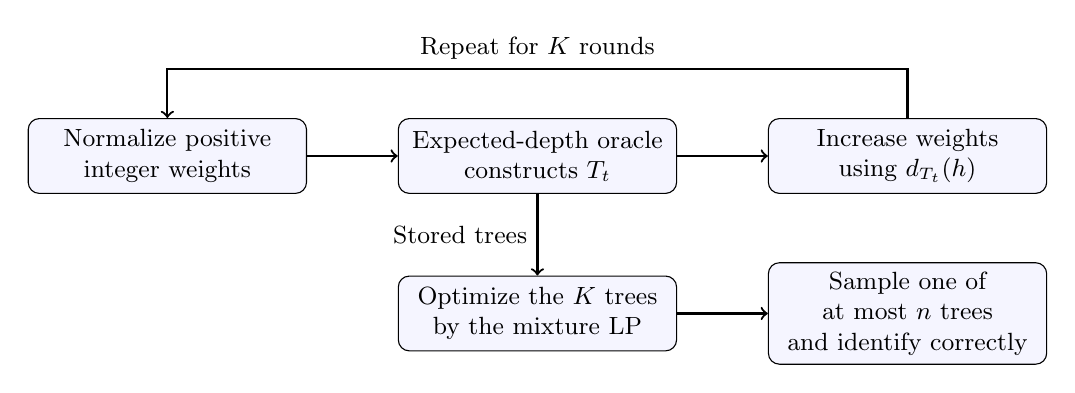
\begin{tikzpicture}[
  box/.style={draw,rounded corners,fill=blue!4,align=center,
              text width=3.3cm,minimum height=0.95cm,font=\small},
  arrow/.style={->,thick},
  every node/.style={font=\small}]
\node[box] (prior) at (0,0) {Normalize positive\\integer weights};
\node[box] (oracle) at (4.7,0) {Expected-depth oracle\\constructs $T_t$};
\node[box] (update) at (9.4,0) {Increase weights\\using $d_{T_t}(h)$};
\node[box] (master) at (4.7,-2) {Optimize the $K$ trees\\by the mixture LP};
\node[box] (sample) at (9.4,-2) {Sample one of at most $n$ trees\\and identify correctly};
\draw[arrow] (prior)--(oracle);
\draw[arrow] (oracle)--(update);
\draw[arrow] (update.north)--(9.4,1.1)--node[above]
  {Repeat for $K$ rounds}(0,1.1)--(prior.north);
\draw[arrow] (oracle)--node[left]{Stored trees}(master);
\draw[arrow] (master)--(sample);
\end{tikzpicture}
\caption{Preprocessing uses the oracle to build trees and the master LP
to choose their probabilities. Each later identification run samples
one complete tree and follows it. Weight updates and the LP run during
preprocessing, before the hidden hypothesis is queried.}
\label{fig:randomized-flow}
\end{figure}

To compare this construction with the best possible randomized
strategy, we first identify its benchmark. The hardest prior is the
dual of the tree-mixture problem: even an ideal mixture must pay
the optimal expected cost of that prior. Since the dual benchmark is
an expected-depth optimum for some prior, an expected-depth
approximation oracle can bound its value in every round.
\begin{proposition}[The comparison game and its entropy lower bound]
\label{prop:randomized-duality}
The optimum in \eqref{eq:randomized-objective} also covers adaptive
zero-error randomized algorithms that terminate almost surely on
every hypothesis. It satisfies
\begin{equation}\label{eq:randomized-duality}
 R^*=\max_{\pi\in\Delta(\HH)}\OPT_E(\pi)
       \ge\log_2n.
\end{equation}
The dual maximum ranges over the full simplex and may assign zero
mass; Algorithm~\ref{alg:randomized-mixture} supplies strictly positive
priors to the expected-depth oracle.
\end{proposition}

The benchmark bounds the oracle's cost on every round's prior.
The regret proposition turns these changing weighted averages into a
bound for \emph{each} hypothesis: a repeatedly slow hypothesis gains
influence until the oracle's weighted cost reflects its depth. The
resulting average-depth bound is for the uniform distribution over
generated trees. Since the restricted master LP also considers this
mixture, its optimized maximum per-hypothesis cost is no greater.
\begin{proposition}[Depth-scaled multiplicative weights]
\label{prop:randomized-regret}
For any sequence of proper oracle trees, let $\pi_t$ be the normalized
weights before round $t$. The uniform mixture of the generated trees
satisfies
\begin{equation}\label{eq:randomized-regret}
 R(\mu^{\rm unif})\le
    (1+\eta)\frac1K\sum_{t=1}^K c_{\pi_t}(T_t)
    +\frac{2L\ln n}{\eta K}.
\end{equation}
\end{proposition}

The uniform mixture in the regret bound may contain many trees.
The master LP keeps its guarantee while producing a concise
strategy. The next proposition also ensures that the repeated
priors and the final random choice can be implemented exactly.
\begin{proposition}[Exact rational construction and sparse optimal mixing]
\label{prop:randomized-compression}
Every iterative prior is strictly positive and rational, with encoding
length polynomial in $n,K$ and the encoding length of $\eta$.
The LP \eqref{eq:randomized-master-lp} is polynomial in size and has an
optimal basic solution supported on at most $n$ trees. Its value is
at most $R(\mu^{\rm unif})$. Its probabilities have polynomial encoding
length and admit exact sampling with an expected polynomial number
of fair random bits. Every sampled query run is correct and uses at
most $n-1$ supplied tests.
\end{proposition}

\begin{proofstrategy}
\begin{enumerate}
\item View hypotheses and legal trees as the two sides of a finite
      game. Its hardest prior lower-bounds every randomized strategy.
\item Increase the weight of hypotheses with large current depths.
      The potential comparison bounds each hypothesis's average
      depth by the oracle's average weighted cost.
\item Optimize the generated mixture by a small LP. The entropy
      lower bound makes the regret term a multiplicative tolerance;
      a basic solution leaves at most $n$ trees to sample.
\end{enumerate}
\end{proofstrategy}

Together, these statements transfer the oracle's approximation
coefficient to the new objective, with a controllable tolerance.
The extra work constructs and mixes trees; the query procedures
inside each tree remain those of the expected-depth oracle.
\begin{theorem}[Transfer to randomized per-hypothesis depth]
\label{thm:randomized-transfer}
For every rational $0<\varepsilon\le1$, Algorithm~\ref{alg:randomized-mixture},
with the calibration at the end of this section, satisfies
\[
 R(\mu)<(\alpha+\varepsilon)R^*\qquad(n\ge2).
\]
It makes $O(n/\varepsilon^2)$ calls to the expected-depth oracle,
uses only positive rational priors, and returns a mixture of at most
$n$ legal trees. If the oracle is polynomial-time in its rational
input, preprocessing is polynomial in the input size and
$1/\varepsilon$. For a singleton, return its leaf with zero queries.
\end{theorem}
\begin{proof}
Proposition~\ref{prop:randomized-duality} and \eqref{eq:randomized-oracle} give
$c_{\pi_t}(T_t)\le\alpha R^*$ in every round. Apply
Proposition~\ref{prop:randomized-regret} and use
$\ln n\le(\ln2)R^*<R^*$ to obtain
\[
 R(\mu^{\rm unif})<
 \left[(1+\eta)\alpha+\frac{2L}{\eta K}\right]R^*.
\]
The final calibration makes the bracket at most
$\alpha+\varepsilon$. Proposition~\ref{prop:randomized-compression} transfers this
bound to the optimized mixture and supplies positivity, legality,
and bit complexity. The chosen $K$ gives the stated number of calls.
\end{proof}

\subsection{Proofs of the supporting propositions}

\subsubsection{The hardest prior is the dual comparison object}

The game interpretation rests on two facts. First, fixing the random
seed turns the policy into a proper tree, and contracting constant
queries can only shorten its paths. Averaging over seeds therefore
gives a tree mixture whose expected depth on each hypothesis is at most
the algorithm's. Second, the mixture optimum equals the expected-depth
cost of its hardest prior. We prove these in order, then use the resulting
lower bound to absorb the weight-update error.

\begin{claim}[Random seeds reduce to a finite proper-tree mixture]
\label{clm:randomized-seed-mixture}
Any zero-error randomized algorithm terminating almost surely on each
hypothesis induces a mixture over $\mathcal T$ whose expected depth on
each hypothesis is at most that of the algorithm.
\end{claim}
\begin{proof}
Condition on a complete random seed. Since $\HH$ is finite, outside
a probability-zero union of events the resulting deterministic
policy terminates correctly on every hypothesis. The union of its
$n$ finite paths is a finite identification tree. Delete unreachable
branches and contract queries constant on their current states.
Every retained query splits a state properly, so the resulting tree
has $n$ leaves, $n-1$ internal nodes, and maximum depth at most $L$.
The finite supplied query family admits only finitely many such
labeled trees. Pushing the seed distribution onto these trees gives
the required mixture. Conversely, sampling any such mixture gives
a legal zero-error strategy.
\end{proof}

After fixing the seed, every strategy is a proper legal tree. The
finite family of these trees defines a mixture LP for the analysis;
its dual assigns mass to hypotheses, giving precisely the prior needed
by the expected-depth oracle. The algorithm constructs a polynomial-size
subset of this finite family, then optimizes the mixture over those trees.
\begin{claim}[Finite LP duality identifies the hardest prior]
\label{clm:randomized-finite-dual}
The finite-tree mixture optimum equals
$\max_{\pi\in\Delta(\HH)}\min_{T\in\mathcal T}c_\pi(T)$.
\end{claim}
\begin{proofstrategy}
We derive the dual by assigning one multiplier to each hypothesis
constraint and one to mixture normalization. The Lagrangian gives the
dual constraints directly; weak duality is then explicit, and finite
LP strong duality completes the equality.
\end{proofstrategy}
\begin{proof}
Write the full mixture LP with one variable $\mu_T$ for each
$T\in\mathcal T$, the depth inequalities, and normalization
$\sum_T\mu_T=1$. Its dual is
\[
 \begin{aligned}
  \text{maximize}\quad&\lambda,\\
  \text{subject to}\quad&
       \lambda\le\sum_h\pi_hd_T(h) &&(T\in\mathcal T),\\
   &\pi_h\ge0,\qquad\sum_h\pi_h=1.
 \end{aligned}
\]
Here one may leave the primal variable $r$ unrestricted: for
$n\ge2$, every depth is at least one, so its inequalities already
force $r\ge1$. To derive the dual, assign nonnegative multipliers
$\pi_h$ to $\sum_T\mu_Td_T(h)-r\le0$ and a free multiplier
$\lambda$ to $1-\sum_T\mu_T=0$. The Lagrangian is
\[
\begin{aligned}
 \mathcal L(r,\mu;\pi,\lambda)
 &=r+\sum_h\pi_h\left(\sum_T\mu_Td_T(h)-r\right)
                      +\lambda\left(1-\sum_T\mu_T\right)\\
 &=r\left(1-\sum_h\pi_h\right)+\lambda
                  +\sum_T\mu_T\bigl(c_\pi(T)-\lambda\bigr).
\end{aligned}
\]
Its infimum over free $r$ and nonnegative $\mu_T$ is finite exactly
when $\sum_h\pi_h=1$ and $c_\pi(T)\ge\lambda$ for every $T$.
Under those conditions the infimum is $\lambda$, giving the stated
dual. In particular, weak duality is visible directly:
\[
 \lambda\le\sum_T\mu_Tc_\pi(T)
       =\sum_h\pi_h\sum_T\mu_Td_T(h)
       \le\sum_h\pi_hr=r.
\]
The first inequality averages the dual constraint over a normalized
mixture. The equality exchanges two finite sums, and the last
inequality weights the primal depth constraints by the nonnegative
$\pi_h$. Their sum is one, which gives the final equality.
The finite primal is feasible and bounded: any proper tree gives
a feasible pure mixture with $1\le r\le L$. Thus
finite LP duality gives equality of its optimum and this dual
optimum. For fixed $\pi$, the largest feasible $\lambda$ is exactly
$\min_Tc_\pi(T)$. The dual permits zero-mass hypotheses because it
defines the comparison benchmark. The algorithm itself uses strictly
positive priors, as required by the oracle.
\end{proof}

The dual identity already gives the comparison benchmark. We also
need its scale: identifying $n$ possibilities requires logarithmic
expected depth under the uniform prior. This ensures that the
additive regret term becomes a multiplicative tolerance.
\begin{claim}[The uniform prior provides a logarithmic lower bound]
\label{clm:randomized-uniform-lower}
Every identifying binary tree has uniform-prior expected depth at
least $\log_2n$.
\end{claim}
\begin{proof}
Its leaf depths satisfy Theorem~\ref{thm:kraft}. By convexity of
$2^{-x}$,
\[
 2^{-\frac1n\sum_hd_T(h)}
   \le\frac1n\sum_h2^{-d_T(h)}\le\frac1n.
\]
The first inequality is Jensen's inequality and the second is Kraft's
bound divided by $n$. Taking $-\log_2$ reverses both inequalities
and gives the claim. Applying Claim~\ref{clm:randomized-finite-dual} to
the uniform prior proves \eqref{eq:randomized-duality}.
\end{proof}

\subsubsection{A weight potential bounds every hypothesis's depth}

Consider a hypothesis that remains slow in many generated trees.
Its weight must grow quickly. The sum of all weights, however,
grows according to the oracle's cost on the current prior. Comparing
these two growth rates bounds every hypothesis's average depth by
the oracle's average weighted cost. Scaling depths by $L$ lets the
same calculation apply to every proper tree.

\begin{claim}[Individual weight growth is paid by total weight growth]
\label{clm:randomized-weight-growth}
For the scaled multiplicative-weights update in
\eqref{eq:randomized-integer-update} and
$g_{h,t}=d_{T_t}(h)/L\in[0,1]$,
\[
 \ln(1+\eta)\sum_{t=1}^Kg_{h,t}
 \le\ln n+\eta\sum_{t=1}^K\sum_g\pi_{g,t}g_{g,t}
 \quad\text{for every }h.
\]
\end{claim}
\begin{proofstrategy}
Remove the common integer factor so the normalized priors are
unchanged. A single hypothesis's weight grows at a rate set by its
depth, while the sum of all weights grows at a rate set by the current
prior's mean depth. Comparing these bounds gives the claim.
\end{proofstrategy}
\begin{proof}
Write $\widehat w_{h,t}=w_{h,t}/(qL)^{t-1}$ for the integer weights
with their common factor removed. This leaves their normalized
prior unchanged and makes their update $1+\eta g_{h,t}$.
Concavity of $x\mapsto\ln(1+\eta x)$ places its graph above the
chord between $x=0$ and $x=1$, giving
$\ln(1+\eta x)\ge x\ln(1+\eta)$, so each final weight obeys
\[
 \ln\widehat w_{h,K+1}\ge\ln(1+\eta)\sum_tg_{h,t}.
\]
For their sum $\widehat W_t$, initially $\widehat W_1=n$ and
\[
 \frac{\widehat W_{t+1}}{\widehat W_t}
    =1+\eta\sum_h\pi_{h,t}g_{h,t}.
\]
Taking logarithms and summing the successive total-weight ratios gives
\[
\begin{aligned}
 \ln\widehat W_{K+1}
 &=\ln n+\sum_{t=1}^K
          \ln\left(1+\eta\sum_g\pi_{g,t}g_{g,t}\right)\\
 &\le\ln n+\eta\sum_{t=1}^K\sum_g\pi_{g,t}g_{g,t}.
\end{aligned}
\]
The inequality uses $\ln(1+x)\le x$ with nonnegative $x$.
For each $h$, positivity and
$\widehat w_{h,K+1}\le\widehat W_{K+1}$ imply
\[
 \ln(1+\eta)\sum_tg_{h,t}
 \le\ln\widehat w_{h,K+1}
 \le\ln\widehat W_{K+1},
\]
which is the required comparison.
\end{proof}

The growth comparison is expressed in normalized depths and
logarithms. For the uniform mixture,
$R(\mu^{\rm unif})=\max_h K^{-1}\sum_t d_{T_t}(h)$; thus rescaling
the claim by $L/K$ converts its per-hypothesis sums to the objective
in \eqref{eq:randomized-objective}. Bounding the two logarithmic
coefficients then gives the explicit regret bound.
\begin{claim}[The potential comparison gives the stated regret]
\label{clm:randomized-regret-rescaling}
Claim~\ref{clm:randomized-weight-growth} implies \eqref{eq:randomized-regret}.
\end{claim}
\begin{proof}
Multiply the bound in Claim~\ref{clm:randomized-weight-growth} by
$L/[K\ln(1+\eta)]$ and maximize over $h$. Since
$\sum_g\pi_{g,t}g_{g,t}=c_{\pi_t}(T_t)/L$, the weighted-depth
term becomes the average oracle cost, and we obtain
\[
 R(\mu^{\rm unif})\le
 \frac{\eta}{\ln(1+\eta)}\frac1K\sum_tc_{\pi_t}(T_t)
 +\frac{L\ln n}{K\ln(1+\eta)}.
\]
The integral for $\ln(1+\eta)$ gives
\[
 \ln(1+\eta)=\int_0^\eta\frac{dx}{1+x}
       \ge\frac{\eta}{1+\eta}\ge\frac{\eta}{2}
       \qquad(0<\eta\le1).
\]
The first inequality bounds the integrand below by its endpoint
value $1/(1+\eta)$; the second uses $1+\eta\le2$.
Therefore
$\eta/\ln(1+\eta)\le1+\eta$ and
$1/\ln(1+\eta)\le2/\eta$. Substituting separately into the
nonnegative mean-cost and error terms gives
\[
 R(\mu^{\rm unif})\le
 (1+\eta)\frac1K\sum_tc_{\pi_t}(T_t)
                  +\frac{2L\ln n}{\eta K},
\]
as claimed.
\end{proof}

\subsubsection{Integer updates and a basic LP solution give a finite strategy}

We analyze the updates with logarithmic potentials and implement them
using positive integer weights; normalization gives the exact rational
priors supplied to the oracle. A basic solution of the master LP bounds
the number of stored trees and the bit length of their probabilities.
Exact sampling then completes the construction and preserves the query
guarantee.

\begin{claim}[All oracle inputs have strictly positive rational weights]
The updates \eqref{eq:randomized-integer-update} preserve positivity
and have polynomial encoding length.
\end{claim}
\begin{proof}
The initial weights are one. Every update factor is a positive
integer at most $(p+q)L$. After $K$ rounds, each weight therefore
has $O(K\log((p+q)L)+1)$ bits. Normalization adds at most
$\lceil\log_2n\rceil$ bits to the denominator. All priors are
strictly positive, so every call meets the oracle's hypothesis.
The generated proper trees have $O(nK)$ total nodes; their depth
matrix consists of integers at most $L$.
\end{proof}

All generated trees can therefore be stored in a polynomial-size
depth matrix. The LP has one column per generated tree and $n$
hypothesis-depth constraints; these constraints determine the worst
expected depth. An optimal basic solution uses this structure to
retain a small support.
\begin{claim}[An optimal basic mixture uses at most $n$ trees]
\label{clm:randomized-basic-support}
The LP \eqref{eq:randomized-master-lp} has an optimal basic solution
with at most $n$ positive tree probabilities and polynomial-bit
rational coefficients.
\end{claim}
\begin{proofstrategy}
Put the LP in standard form and use positivity of the objective
variable to bound the number of tree probabilities in a basic
solution. Then bound the basis determinants to control the bit length
of those probabilities.
\end{proofstrategy}
\begin{proof}
Its uniform mixture is feasible. Replacing every depth inequality
by
\[
 \sum_t\mu_td_{T_t}(h)+s_h-r=0,\qquad s_h\ge0,
\]
gives standard form with $n+1$ equalities and nonnegative variables
$\mu_t,s_h,r$. Because $n\ge2$, every proper tree has depth at least
one on every hypothesis. Since the probabilities sum to one, each
depth inequality therefore forces $r\ge1$, so the variable $r$ is
positive in every feasible solution. A basic solution has at most
$n+1$ positive variables, leaving at most
$n$ for tree probabilities. If some equalities are dependent, the basis
dimension decreases and the same support bound remains valid. A finite
optimal basic solution exists, and its
integer basis matrix has entries of absolute value at most $L$.
For completeness, let $b\le n+1$ be the basis size. The basis
matrix $B$ is nonsingular and integer, so $|\det B|\ge1$.
Each of its columns has Euclidean norm at most $\sqrt b\,L$.
Hadamard's bound and Cramer's rule therefore give
\[
 1\le|\det B|\le(\sqrt b\,L)^b,\qquad
 |\det B_i|\le(\sqrt b\,L)^b,\qquad
 x_i=\frac{\det B_i}{\det B}.
\]
The bound on $B_i$ also holds because the right-hand side has
entries zero or one, and $L\ge1$. Each numerator and denominator
thus needs $O(b(\log b+\log L)+1)$ bits. In particular the tree
probabilities have polynomial encoding length. Rational LP algorithms,
followed by exact basis extraction on the optimal face, find such
an optimal basic solution in polynomial time
\cite{khachiyan1979}. The uniform mixture is feasible, so the optimized
value is at most $R(\mu^{\rm unif})$.
\end{proof}

The sparse LP solution assigns probabilities to the retained trees.
Each run samples one tree and executes it from root to leaf. Its
rational probabilities allow an exact draw using fair bits, so the
execution preserves the zero-error query guarantee.
\begin{claim}[The compressed mixture is exactly sampleable]
\label{clm:randomized-exact-sampling}
The optimized rational mixture gives a legal zero-error execution
with at most $L$ queries and expected polynomial sampling cost.
\end{claim}
\begin{proofstrategy}
Clear the rational probabilities to obtain integer interval lengths.
Rejection sampling produces a uniform integer in their common range,
which selects a tree with exactly its LP probability and finite
expected bit cost.
\end{proofstrategy}
\begin{proof}
By Claim~\ref{clm:randomized-basic-support}, take a common denominator
$D$ for its at most $n$ polynomial-bit probabilities;
its encoding length is polynomial. Explicitly, if their denominators
are $b_1,\ldots,b_s$, take $D=\prod_{i=1}^s b_i$; then
$\log_2D=\sum_i\log_2b_i$ is polynomial. Writing the probabilities
as $a_i/D$ gives nonnegative integer interval lengths with
$\sum_i a_i=D$. Draw a uniform integer from
$\{0,\ldots,D-1\}$ by fair bits and rejection, then use the
cumulative integer probability intervals. Rejection makes every
accepted integer equiprobable, so an interval of length $a_i$ has
probability $a_i/D$. If $D=1$, select the sole supported tree
deterministically. Otherwise each attempt uses
$\lceil\log_2D\rceil$ bits and is accepted with probability
greater than $1/2$, so the expected number of attempts is less
than two: with $b=\lceil\log_2D\rceil$, each $b$-bit draw is uniform
on $\{0,\ldots,2^b-1\}$, and
$D/2^b>1/2$. Conditioning on a draw below $D$ makes it uniform
on the desired range.
The sampled tree identifies every hypothesis and has
depth at most $L$. This completes the compression proposition.
\end{proof}

The two optimization viewpoints also give a useful stopping
certificate. The restricted master LP supplies an upper bound on
$R^*$ because its mixture is a feasible strategy, while
\[
 \max_t\frac{c_{\pi_t}(T_t)}\alpha\le R^*
\]
supplies a lower bound by \eqref{eq:randomized-oracle} and
\eqref{eq:randomized-duality}. Their ratio is an instance-specific
certificate. Stop early when it meets the desired factor; otherwise,
the fixed-round guarantee still applies.

\subsection{Calibration and the strongest resulting guarantees}

The preceding proof separates the oracle's approximation loss from
the loss due to finitely many weight-update rounds. Split the desired
tolerance equally between these two terms; the following choices
make that split explicit.

\begin{parameterchoice}
For a fixed rational oracle coefficient $\alpha\ge1$ and target
$0<\varepsilon\le1$, choose
\begin{equation}\label{eq:randomized-calibration}
 \eta=\frac{\varepsilon}{2\alpha},\qquad
 K=\left\lceil\frac{8\alpha(n-1)}{\varepsilon^2}\right\rceil.
\end{equation}
The definition of $\eta$ gives $\alpha\eta=\varepsilon/2$. For the
second term, use $L=n-1$ and the lower bound on the ceiling-defined $K$:
\[
 \frac{2L}{\eta K}
 \le \frac{2L}{(\varepsilon/(2\alpha))(8\alpha L/\varepsilon^2)}
 =\frac{\varepsilon}{2}.
\]
Thus each error term is at most $\varepsilon/2$, and their sum is at
most $\varepsilon$.
\end{parameterchoice}

The oracle and duality give
$c_{\pi_t}(T_t)\le\alpha\OPT_E(\pi_t)\le\alpha R^*$ in each round.
Substitution into the regret inequality yields
\[
\begin{aligned}
 R(\mu^{\rm unif})
 &\byref{Prop.}{prop:randomized-regret}{\le}
 (1+\eta)\alpha R^*+\frac{2L\ln n}{\eta K}\\
 &\byref{Eq.}{eq:randomized-calibration}{\le}
 \left(\alpha+\frac{\varepsilon}{2}\right)R^*
                      +\frac{\varepsilon}{2}\ln n\\
 &\byref{Prop.}{prop:randomized-duality}{<}(\alpha+\varepsilon)R^*.
\end{aligned}
\]
The final inequality is strict because $n\ge2$ and
$\ln n=(\ln2)\log_2n<\log_2n\le R^*$.
The optimized mixture has cost at most that of the uniform one.

The current expected-depth certificate in
Section~\ref{sec:two-phase} gives the rational valid oracle
coefficient $\alpha=5.18297551$. Choosing
$\varepsilon=1/4000000$ in the single mixture algorithm yields
\[
 R(\mu)<5.18297576\,R^*<5.182976\,R^*.
\]
This is the best polynomial factor established here for the
randomized per-hypothesis objective. The small tolerance makes the
iteration constant large; the parameterized theorem and the
optimized master LP allow more practical tolerance choices.

Using a stronger expected-depth oracle preserves the prior updates and
mixture LP while improving the guarantee for this randomized objective.
The quasipolynomial oracle gives the stronger factor, and its running
time carries over to preprocessing.
\begin{corollary}[Quasipolynomial randomized per-hypothesis approximation]
\label{cor:randomized-quasipolynomial}
For every fixed rational $\varepsilon>0$, the same LP-compressed
mixture algorithm has a supplied-query quasipolynomial
$(2+\varepsilon)$ approximation for $R^*$. For
$0<\varepsilon\le1$, its time is
$(mn)^{O(\varepsilon^{-1}\log n)}$ times a polynomial in input
bit length, and its mixture is supported on at most $n$ trees.
\end{corollary}
\begin{proof}
Use the expected-depth oracle of
Theorem~\ref{thm:qp-two-plus-epsilon} with coefficient
$\alpha=2+\varepsilon/2$, and apply the transfer theorem with
tolerance $\varepsilon/2$. The factor is strictly below
$2+\varepsilon$ for $n\ge2$. There are
$\lceil32\alpha(n-1)/\varepsilon^2\rceil$ oracle calls, whose
positive rational priors have polynomial encoding length. These
calls and the master LP preserve the oracle's stated
quasipolynomial running-time form. For $\varepsilon>1$, use
$\varepsilon=1$; a singleton again returns its leaf.
\end{proof}

\section{Allowing hypotheses on supplied lines}
\label{sec:boundaries}

Allowing a hypothesis to lie on a queried line adds a third outcome.
To compare with the binary algorithms, encode each line answer using
at most two bits: the first separates zero from nonzero, and the
second separates negative from positive on the nonzero branch. Thus
each ternary query expands to at most two levels in a binary comparison
tree, which accounts for the factor of two in the guarantee.

Algorithm~\ref{alg:boundary} implements the reduction below.
In this section a supplied line returns one of three answers:
negative, zero, or positive. The \emph{zero}, or \emph{on-line},
answer means the hypothesis lies on the queried line, and its
answer class is $S_\ell^0=\{h\in S:f_\ell(h)=0\}$.
A \emph{ternary decision tree} has an outgoing edge for each
possible answer; a proper such tree retains only nonempty outcomes.
Leaf depths and both cost objectives use the same conventions as in
the binary model.
Use the two virtual binary predicates
\[
 b_1(h)=\mathbf1[f_\ell(h)<0],\qquad
 b_2(h)=\mathbf1[f_\ell(h)\le0].
\]
Their pair of bits distinguishes the three outcomes.
In the order $(b_1,b_2)$, negative, zero, and positive signs map to
$(1,1)$, $(0,1)$, and $(0,0)$, respectively; the unused pair $(1,0)$
never occurs. Thus no outcome is merged, and the virtual binary tree
can omit the unused branch at each query.
Requesting either bit is implemented by querying the original line
once and storing its full sign. Both bits are then known. For analysis
we count each requested virtual bit as a separate binary query;
the actual number of supplied-line queries can only be smaller.

For preprocessing, we also represent these bit labelings by planar
queries whose lines avoid every hypothesis. On the finite hypothesis
set, sufficiently small shifts preserve both bit values while moving
the virtual boundaries off the points. During execution, the algorithm
asks the original supplied line and reads its full ternary sign, so
the virtual representation changes only the analysis and preprocessing.
Any query whose answer is constant on the hypothesis set can be
discarded. For every remaining query, choose $\epsilon_\ell$ to be
half the minimum nonzero $|f_\ell(h)|$ on the finite hypothesis set.
At least one such nonzero value exists because the query is not
constant (a nonconstant sign labeling must contain a nonzero value).
For a rational input instance, this minimum is computable by scanning
the hypotheses and has polynomial encoding length: evaluating an
input affine form and taking the minimum of finitely many rational
absolute values preserves polynomial bit length. Then $b_1$ is represented
by $f_\ell(x)<-\epsilon_\ell$ and $b_2$ by
$f_\ell(x)<\epsilon_\ell$. These strict inequalities agree with the
definitions on every
hypothesis: a negative nonzero value is at most $-2\epsilon_\ell$,
and a positive value is at least $2\epsilon_\ell$, while zero lies
between the two thresholds. In particular, neither shifted boundary
contains a hypothesis. The shifts are used only for preprocessing;
their answers are obtained from the original supplied line.

\begin{symboltable}
$f_\ell(h)$ & Affine value whose sign is the answer for hypothesis $h$.\\
$b_1(h),\ b_2(h)$ & Virtual bits for $f_\ell(h)<0$ and $f_\ell(h)\le0$; together they encode the ternary sign.\\
$\epsilon_\ell$ & Positive shift smaller than every nonzero $|f_\ell(h)|$ on the finite hypothesis set.
\end{symboltable}

\begin{algorithm}[H]
\caption{Transfer a binary algorithm to on-line outcomes}
\label{alg:boundary}
\KwIn{Finite hypotheses, supplied ternary lines, binary tree-construction routine $B$.}
\KwOut{An executable tree using the original supplied lines.}
\ForEach{nonconstant supplied line $\ell$}{
  $\epsilon_\ell\gets\frac12\min_{h:f_\ell(h)\ne0}|f_\ell(h)|$\;
  Represent virtual bits $b_1=\mathbf1[f_\ell(h)<0]$ and
  $b_2=\mathbf1[f_\ell(h)\le0]$ by the two shifted off-boundary lines\;
}
Construct a virtual binary tree with $B$\;
Execute a requested virtual bit by querying its original line,
caching the entire ternary sign; answer further requests from that cache\;
\KwRet the contracted original-line tree\;
\end{algorithm}

Lines constant on the whole hypothesis set are discarded before taking
the minimum nonzero affine value. Proposition~\ref{prop:boundary}
proves that the approximation ratio increases by at most two.


There are two comparisons to make. An optimal ternary tree can be
simulated using at most two virtual bits per query. A constructed
virtual tree can then be executed using original line queries,
with the cached sign supplying both bits whenever either is asked.
Because the first comparison bounds each hypothesis's virtual depth
by twice its original depth, and the second bounds each executed depth
by that hypothesis's virtual depth, both comparisons survive either
taking a maximum or summing depths with nonnegative prior weights.
\begin{proposition}[Boundary reduction]\label{prop:boundary}
An $\alpha$-approximation for either binary objective gives a
$2\alpha$-approximation for the corresponding three-answer objective.
\end{proposition}
\begin{proof}
Simulate every query of an optimal original tree by its two virtual
bits. Each hypothesis uses at most twice as many binary queries,
so the virtual optimum is at most twice the original optimum
for either objective. Conversely, execute a constructed virtual
tree by original line queries and cached signs. Its actual depth
is no larger than its virtual depth on every hypothesis.
To combine these comparisons explicitly, write $C_{\rm orig}$ for
the executed cost and $\OPT_{\rm virt},\OPT_{\rm orig}$ for the two
optima. Then, for either depth objective,
\[
 C_{\rm orig}\le C_{\rm virt}
 \le\alpha\OPT_{\rm virt}\le2\alpha\OPT_{\rm orig}.
\]
The first step uses cached-sign execution, the second is the assumed
binary approximation guarantee, and the last uses the two-bit
simulation of the optimal ternary tree. Thus the comparison applies
to both maximum depth and any weighted sum of leaf depths.
\end{proof}

The reduction is independent of the binary algorithm's internal
geometry or schedule. Applying it to the strongest deterministic
algorithms established above gives the following bounds for the
model with on-line outcomes.
\begin{corollary}[Constant approximations with on-line outcomes]
\label{cor:constant-boundaries}
With on-line answers, expected depth has a polynomial-time
approximation factor below $10.365952$ for arbitrary positive priors,
and deterministic maximum depth has a factor below $8.929931$.
\end{corollary}
\begin{proof}
Apply Proposition~\ref{prop:boundary} to
Theorems~\ref{thm:two-phase-expected} and~\ref{thm:poly-slot-worst}.
\end{proof}

\section{Strong NP-completeness}
\label{sec:hardness}

The approximation algorithms exploit planar structure, but exact
optimization remains hard. We first state the decision and source
problems and the graph terminology used by both reductions.

\begin{definition}[Complexity and reductions]\label{def:complexity}
A \emph{polynomial-time many-one reduction} maps instances of one
decision problem to another in polynomial time, so an input is a
yes-instance if and only if its image is a yes-instance.

A decision problem is in \emph{NP} if every yes-instance has a
certificate of polynomial encoding length whose validity is
checkable in polynomial time, and no certificate is accepted on a
no-instance. It is \emph{NP-hard} if every problem
in NP admits such a reduction to it, and \emph{NP-complete} if it
is both NP-hard and in NP.
A numerical problem is \emph{strongly NP-hard} if hardness persists
when its integer data are bounded by a fixed polynomial in the
combinatorial instance size; it is \emph{strongly NP-complete} if
it is also in NP. For rational data, our restricted instances
explicitly bound both numerators and denominators.
\end{definition}

\begin{definition}[3-Partition]\label{def:three-partition}
The input consists of positive integers $a_1,\ldots,a_m,B$, where
$m=3p$ for a positive integer $p$, satisfying
\[
 s=\sum_{i=1}^m a_i=pB,\qquad B/4<a_i<B/2.
\]
The question is whether $[m]$ can be partitioned into $p$ groups
$I_1,\ldots,I_p$ with $|I_b|=3$ and
$\sum_{i\in I_b}a_i=B$ for every $b$.
\end{definition}

\begin{symboltable}
$m=3p,\ [m]$ & Number of source items and their index set.\\
$a_i,\ B$ & Item size $i$ and target sum of each bin.\\
$s=pB=\sum_i a_i$ & Total item size and total capacity of the $p$ bins.\\
$I_b$ & Index set of the three items assigned to source bin $b$.\\
\end{symboltable}

Both reductions use the strong NP-completeness of this
problem~\cite{gj1979}.
We use the NP-hard restriction in which $B$ is polynomially bounded
in $m$. The case $p=1$ is a trivial yes-instance, so excluding it
preserves NP-hardness. In this restriction each $a_i$ is
polynomially bounded, so the explicit
repetitions in our constructions remain polynomial in the source
size. A partition into $p$ groups of sum $B$
then necessarily has three items per group: two items sum to less
than $B$, while four items sum to more than $B$.

\begin{definition}[Paths and matchings]\label{def:paths-and-matchings}
A \emph{path} is an undirected graph with distinct vertices
$v_0,\ldots,v_k$ and edges exactly
$\{v_{j-1},v_j\}$ for $1\le j\le k$.
A \emph{linear forest} is a disjoint union of paths, allowing
isolated vertices. Throughout, an \emph{odd path} has an odd number
of vertices; when its edge count matters, we state that count
explicitly. Positions are numbered locally from zero along each item
path, separately from global hypothesis indices.

A \emph{matching} is a set of edges with no shared endpoint.
A vertex is \emph{unmatched} if it is incident to no chosen edge.
A \emph{maximum matching} has the largest possible number of edges.
A \emph{perfect matching} leaves no vertex unmatched.
\end{definition}

Both reductions turn the same source decision into a choice of one bin
for each item. To represent those choices, we place an item on an odd
path and supply tests for each vertex and each adjacent pair. The
distinguished hypothesis forces an optimal tree to use a maximum
matching of these pair tests; by Lemma~\ref{lem:odd-path}, the one
unmatched even-position vertex then specifies the item's bin. This
Each unmatched-position choice changes a different statistic. For
maximum depth, clouds change the number of branches at each height;
for expected depth, weights change the pair-mass histogram. Summing
these statistics across the items recovers the source bin loads.
Finally, the parabola realizes every singleton and adjacent-pair test
as a supplied line, and the cloud replacement in
Section~\ref{sec:uniform-hardness} transfers the weighted expected-depth
instance to a uniform prior while adding the same fixed internal cost
to every maximum matching.

\subsection{The geometric realization and the matching choice}

For integer abscissae, the line
\[
 I_{a,b}:\quad
 4y-4(a+b)x+(2a-1)(2b+1)=0
\]
has value $4(x-a+\tfrac12)(x-b-\tfrac12)$ on $(x,x^2)$.
Its negative answer selects exactly the integer abscissae
$a,\ldots,b$. This realizes interval membership using one line.
The line
\begin{equation}\label{eq:private-singleton}
 P_t:\quad 2y-4tx+2t^2-1=0
\end{equation}
has value $2(x-t)^2-1$, and its negative answer isolates exactly
the point of abscissa $t$. Both formulas are nonzero at all integer
abscissae, so every answer is binary.
The tangent $y=2tx-t^2$ exposes the point $(t,t^2)$, since every
other parabola point lies strictly above it. The constructed
hypotheses are therefore in strictly convex position.

We use the negative answer class of each displayed line as its
membership set. Consequently, a hit in
Definition~\ref{def:membership-spine} is precisely a negative affine
sign, while the distinguished hypothesis is placed outside every such
set. This convention lets the combinatorial path tests above enter the
membership-spine framework without changing the supplied queries.



With this membership convention, the two formulas realize every
singleton and adjacent-pair test used by the matching construction.
The parabola keeps all hypotheses exposed on the convex hull, and the
integer abscissae give explicit integer coefficients for each line.
Figure~\ref{fig:parabola-queries} illustrates $I_{2,5}$ and $P_4$ on
the points with integer abscissae from $0$ to $8$.

\begin{figure}[tbp]
\centering
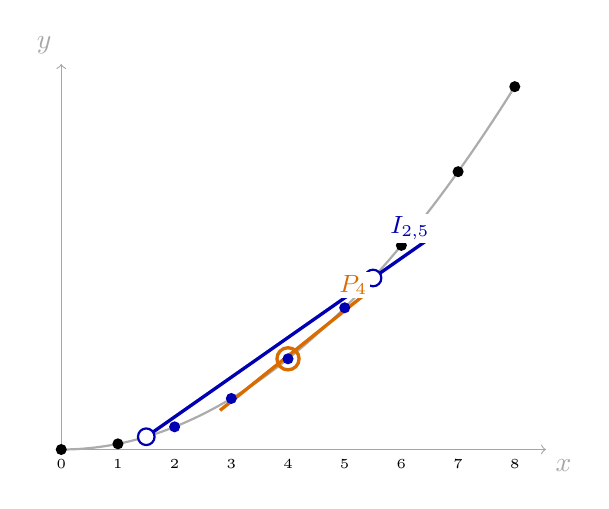
\begin{tikzpicture}[x=0.72cm,y=0.072cm]
  \draw[->,gray!70] (0,0)--(8.55,0) node[below right] {$x$};
  \draw[->,gray!70] (0,0)--(0,68) node[above left] {$y$};
  \foreach \x in {0,...,8} {
    \node[below,font=\tiny] at (\x,0) {\x};
  }
  \draw[thick,gray!65] plot[domain=0:8,samples=81] (\x,{(\x)^2});
  \draw[very thick,blue!70!black]
    plot[domain=1.5:6.5,samples=60] (\x,{7*\x-8.25});
  \draw[very thick,orange!85!black]
    plot[domain=2.8:5.4,samples=50] (\x,{8*\x-15.5});
  \draw[blue!70!black,fill=white,thick] (1.5,2.25) circle (3pt);
  \draw[blue!70!black,fill=white,thick] (5.5,30.25) circle (3pt);
  \foreach \x in {0,1,6,7,8} {
    \pgfmathsetmacro{\yy}{\x*\x}
    \fill[black] (\x,\yy) circle (2pt);
  }
  \foreach \x in {2,3,4,5} {
    \pgfmathsetmacro{\yy}{\x*\x}
    \fill[blue!70!black] (\x,\yy) circle (2pt);
  }
  \draw[orange!85!black,very thick] (4,16) circle (4pt);
  \node[font=\small,text=blue!70!black,fill=white,inner sep=1pt]
    at (6.15,39) {$I_{2,5}$};
  \node[font=\small,text=orange!85!black,fill=white,inner sep=1pt]
    at (5.15,29) {$P_4$};
\end{tikzpicture}
\caption{The integer points lie on $y=x^2$. The blue line
$I_{2,5}$ has negative answer exactly on the points with
$x\in\{2,3,4,5\}$; the orange line $P_4$ has negative answer only
at $x=4$, marked with an orange ring. The interval endpoints are
the half-integer intersections $x=1.5$ and $x=5.5$.}
\label{fig:parabola-queries}
\end{figure}

For maximum depth we also use \emph{clouds} of ordinary points.
They make a local identification problem take a chosen number of
queries without changing the objective. A cloud's size $w_i$ counts
its hypotheses in this maximum-depth construction.
Given positive integer cloud sizes $w_i$, put $Q=4\max_i w_i$
and represent cloud $i$ by
\[
 \{(Qi+j,(Qi+j)^2):0\le j<w_i\}.
\]
Its point with $j=0$ is its \emph{anchor}. Supply the cloud-interval line
\begin{equation}\label{eq:cloud-interval}
 4y-4Q(a+b)x+Q^2(2a-1)(2b+1)=0.
\end{equation}
For $a\ge1$ its negative answer selects exactly the clouds
$a,\ldots,b$, while excluding cloud $0$.
This follows by factoring its value as
$4(x-Q(a-\tfrac12))(x-Q(b+\tfrac12))$.
Each cloud lies within $Q/4$ of its anchor, so neither boundary,
halfway between consecutive anchors, contains a hypothesis.
Each nonanchor point receives a private line
\eqref{eq:private-singleton}. The anchors use only cloud tests: an
anchor and a point in its own cloud agree on every cloud-interval test
and on every other private test. Their separation therefore requires
the point's own private query. Thus a cloud of size $w$ forces $w-1$
queries on the anchor's local path, while the anchor remains available
to represent the cloud in the matching construction.

Clouds are ordered so that consecutive vertices of each path used
below have consecutive cloud indices. The only cloud-interval tests
are whole-cloud singleton tests and adjacent-pair tests specified
by those paths. Every point, including every anchor, must be identified.

The matching construction uses clouds as exits with prescribed
local heights. The following exact values let the later histogram
account for those exits without making assumptions about their
internal adaptive trees.

\begin{lemma}[Identifying one or two clouds]\label{lem:cloud-heights}
For this supplied family, the minimum height on one cloud of size $w$
is $w-1$. On two clouds of sizes $u,v$, when their whole-cloud
singleton tests are supplied, the minimum height is $\max\{u,v\}$.
\end{lemma}
\begin{proof}
On a single cloud, old cloud-interval tests are constant and each
private test isolates one nonanchor point. The anchor answers the
same way as every nonanchor on all the other private tests, so its
path must ask all $w-1$ of them. Querying them sequentially achieves
that height.

On two clouds, the anchor of the larger cloud must use all its
private tests: each is the only query separating that cloud's anchor
from its corresponding nonanchor. It must also use at least one
cloud-interval test, since private tests give the same answer at
both anchors. The larger cloud therefore forces depth at least
$\max\{u,v\}$.
First separating the clouds and then performing their private
searches attains the bound.
\end{proof}

Each odd item path encodes one bin choice. Its single unmatched vertex
fixes the entire remaining matching, so that position identifies the
chosen bin.

\begin{lemma}[One unmatched position]\label{lem:odd-path}
A maximum matching of the path
\[
 E_0,B_1,E_1,\ldots,B_t,E_t
\]
leaves exactly one vertex $E_k$ unmatched. It then uses pairs
$\{E_{j-1},B_j\}$ for $j\le k$ and
$\{B_j,E_j\}$ for $j>k$.
\end{lemma}
\begin{proof}
There are $2t+1$ vertices, so a matching contains at most $t$ edges.
Taking the pairs $\{E_{j-1},B_j\}$ for $j=1,\ldots,t$ attains this
bound; hence every maximum matching covers $2t$ vertices and leaves
one vertex unmatched. If that vertex is at position $r$ along the
path, the $r$ vertices before it and the $2t-r$ vertices after it
are both covered by matching edges wholly within their respective
segments. Both segment sizes are therefore even, so $r$ is even;
write $r=2k$, making the unmatched vertex $E_k$.

The left segment now begins at endpoint $E_0$, whose only available
neighbor is $B_1$. Thus its first pair is forced to be
$\{E_0,B_1\}$; after removing that pair, the same endpoint argument
forces $\{E_1,B_2\}$, and so on through $\{E_{k-1},B_k\}$. Reading
the right segment from endpoint $E_t$ forces, in turn,
$\{B_t,E_t\},\ldots,\{B_{k+1},E_{k+1}\}$. These are precisely the
pairs in the statement, and each was forced by the endpoint of its
remaining segment.
\end{proof}

Figure~\ref{fig:odd-path-matching} shows the smallest nontrivial
example of the matching pattern. Moving the unmatched even-position
cloud changes which segment represents the item's bin choice.
\begin{figure}[tbp]
\centering
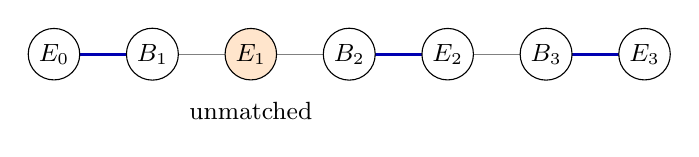
\begin{tikzpicture}[every node/.style={font=\small}]
  \draw[gray] (0,0)--(7.5,0);
  \draw[very thick,blue!70!black] (0,0)--(1.25,0);
  \draw[very thick,blue!70!black] (3.75,0)--(5,0);
  \draw[very thick,blue!70!black] (6.25,0)--(7.5,0);
  \node[draw,circle,fill=white,inner sep=2pt] at (0,0) {$E_0$};
  \node[draw,circle,fill=white,inner sep=2pt] at (1.25,0) {$B_1$};
  \node[draw,circle,fill=orange!20,inner sep=2pt] at (2.5,0) {$E_1$};
  \node[draw,circle,fill=white,inner sep=2pt] at (3.75,0) {$B_2$};
  \node[draw,circle,fill=white,inner sep=2pt] at (5,0) {$E_2$};
  \node[draw,circle,fill=white,inner sep=2pt] at (6.25,0) {$B_3$};
  \node[draw,circle,fill=white,inner sep=2pt] at (7.5,0) {$E_3$};
  \node[below=14pt] at (2.5,0) {unmatched};
\end{tikzpicture}
\caption{A maximum matching of
$E_0,B_1,E_1,B_2,E_2,B_3,E_3$ with $E_1$ left unmatched.
Blue edges are the selected adjacent pairs. In the reduction, the
unmatched even-position cloud selects the item's bin; the uniquely
forced pairs lie to its left and right.}
\label{fig:odd-path-matching}
\end{figure}

The item paths only organize the supplied membership queries. The
reduction uses singleton and adjacent-pair tests directly; no
underlying edge-query search tree is part of the instance.

\subsection{Maximum depth: bin loads become branch-height counts}

\begin{theorem}[Strong NP-completeness of maximum depth]
\label{thm:strong-worst}\label{thm:strong-height}
Deciding whether $\OPT_W(\HH)\le K$ is strongly NP-complete,
even for integer-coordinate points on a parabola, polynomially bounded
integer line coefficients, and $O(n)$ supplied binary line queries.
\end{theorem}

\begin{proofstrategy}
\begin{enumerate}
\item Force the distinguished anchor's path to attain its minimum
length. Its first-hit pairs must then be a maximum matching, with
one even-position cloud unmatched in each item path.
\item Use local cloud heights and a sorted exit histogram to exclude
internal unmatched positions. Each remaining boundary is one bin choice.
\item Moving that boundary transfers the item's size between disjoint
histogram windows. The height threshold requires every bin load to be
at most $B$, hence exactly $B$.
\end{enumerate}
\end{proofstrategy}

\subsubsection{Construction and supporting propositions}

Use the restricted 3-Partition instance of Definition~\ref{def:three-partition}.
Let $q=(p-1)(4s+2m)$ be the total matching size and $T=s-B$ the
width of a bin window. Choose a cloud offset $M$, bin levels
$\lambda_1,\ldots,\lambda_p$, and high cloud sizes $H,C$ by the
calibration in Section~\ref{sec:height-hardness-calibration}; the
decision threshold is $K=q+M$.
The source information is $a_i,B,p$; these additional quantities only
separate branch-height levels and make the distinguished path tight.

For item $i$, construct an odd path whose vertices represent clouds.
Starting with an even-position cloud of size $2$, append $p-1$
segments, indexed by $b=1,\ldots,p-1$. Each row below appends an
odd-position cloud and then the next even-position cloud.
Segment $b$ consists of one entry row, $a_i$ repetitions of the
four block rows, and one exit row:
\[
 \begin{array}{c|c|c}
 \text{part}&\text{odd-position size}&\text{next even size}\\ \hline
 \text{entry}&C&M\\
 \text{block step 1}&\lambda_b&H\\
 \text{block step 2}&\lambda_b+T&M\\
 \text{block step 3}&\lambda_{b+1}+T&H\\
 \text{block step 4}&\lambda_{b+1}&M\\
 \text{exit}&C&2
 \end{array}
\]
The repeated block is the only part depending on $a_i$.
It transfers $a_i$ units between neighboring histogram windows.
There are $4a_i+2$ odd-position vertices per segment, so the
whole item path has $2s_i+1$ vertices, where
$s_i=(p-1)(4a_i+2)$, and its maximum matching has size $s_i$.
Its $p$ even-position clouds of size $2$ are the segment boundaries.

Add one auxiliary cloud of size $M$ and cloud $0$ of size $2$.
Supply each nonzero cloud's whole-cloud singleton test, each
adjacent-pair test within an item path, and each nonanchor point's
private singleton test. Realize them by \eqref{eq:cloud-interval}
and \eqref{eq:private-singleton}.


For boundary choices, let $L_b$ be the total item size assigned to bin
$b$. Put
\[
 Q_{\mathrm{hi}}=2(p-1)(s+m),\qquad
 \beta_1=q-s,\qquad
 \beta_b=Q_{\mathrm{hi}}+2s(p-b)\quad(2\le b\le p).
\]
Here $Q_{\mathrm{hi}}$ counts the always-high pairs, and $\beta_b$
is the reference tail count in bin window $b$ after its bin load is
removed. These counts are combinatorial; their levels are calibrated later.

Soundness starts with an arbitrary adaptive tree. A tight lower
bound on the distinguished path forces its cloud groups to form
maximum matchings; only then can their heights be sorted and counted.

\begin{proposition}[Tight-spine matching normalization]
\label{prop:height-normalization}
Every identifying tree has height at least $K$. A tree of height at
most $K$ can be normalized without increasing height so its first-hit
pairs form a maximum matching in every item path, all clouds are
intact at their first hit, and the distinguished cloud's private query
is last. If $N(t)$ counts exits of local height at least $t$, sorting
those exits by nonincreasing height gives the exact criterion
\begin{equation}\label{eq:height-profile}
 t+N(t)\le K
\end{equation}
at every exit-height level.
\end{proposition}

The odd-path lemma allows every even position to be unmatched,
but only the designated boundaries should represent bins. One height
level detects and excludes all internal positions at once.

\begin{proposition}[Only boundary positions are feasible]
\label{prop:height-boundaries}
Every matching whose normalized tree fits height $K$ leaves a
boundary cloud unmatched in each item path. Its $p$ possible boundaries choose the item's bin.
\end{proposition}

With internal positions excluded, moving an unmatched boundary is
a genuine bin choice. Its effect on the exit histogram adds across
items, turning the height constraints into bin-capacity constraints.

\begin{proposition}[Histogram windows encode bin loads]
\label{prop:height-windows}
At the upper level $t_b=\lambda_b+T$ of each bin window,
\[
 N(t_b)=\beta_b+L_b,\qquad t_b+\beta_b=K-B.
\]
Consequently the height criterion requires $L_b\le B$ for every bin.
\end{proposition}

The bin windows establish the necessary conditions. For the reverse
direction, balanced loads must also respect every remaining height
level and identify all cloud points, including the distinguished cloud.

\begin{proposition}[Balanced loads give a complete tree]
\label{prop:height-completeness}
Boundary matchings with $L_b=B$ satisfy every height-profile constraint
and yield a complete identifying tree of height $K$.
\end{proposition}

The combinatorial equivalence must be accompanied by a size bound.
Explicit clouds and integer lines preserve strong hardness only if
their replication and numerical values stay polynomial.

\begin{proposition}[Polynomial geometric encoding]
\label{prop:height-encoding}
The construction has polynomial size on the restricted source input,
integer coordinates and coefficients bounded by $O(n^4)$, and $O(n)$
supplied strict binary lines. A height-$K$ identifying tree is a
polynomially checkable NP certificate.
\end{proposition}

\begin{proof}[Proof of Theorem~\ref{thm:strong-worst}]
A source partition yields a height-$K$ tree by
Proposition~\ref{prop:height-completeness}. Conversely, normalize any
height-$K$ tree by Proposition~\ref{prop:height-normalization};
Propositions~\ref{prop:height-boundaries} and~\ref{prop:height-windows}
give bin loads at most $B$. Since their sum is $s=pB$ across $p$ bins,
every load must equal $B$. Each such bin contains three items: two
items sum to less than $B$, while four sum to more than $B$, by the
source promise $B/4<a_i<B/2$. These groups form a 3-partition.
Proposition~\ref{prop:height-encoding} supplies strong polynomial
encoding and NP membership. Thus the reduction is exact for arbitrary
adaptive trees.
\end{proof}

\subsubsection{Technical proofs of the height propositions}

\begin{proof}[Proof of Proposition~\ref{prop:height-normalization}]
We normalize in two stages. First, counting the queries unavoidable
on the distinguished anchor's path forces maximum matchings and intact
cloud exits. Then sorting those exits gives the complete height test.

\begin{claim}[The distinguished anchor forces maximum matchings]
\label{clm:height-tight-anchor}
Every identifying tree has height at least $K$. If its height is at
most $K$, the first-covered pairs form a maximum matching in every
item path, and no nonzero-cloud private test is asked on the anchor
path.
\end{claim}
\begin{proof}
Follow the anchor of cloud $0$ through any complete tree. It needs the private
test for the other point of cloud $0$. Private tests of other
clouds do not distinguish their anchors from this anchor.
It therefore also needs cloud queries covering the $2q+m$ item-path
anchors and the auxiliary anchor.

Classify each anchor by its first hitting cloud query along this
all-miss path. A query first covers one anchor or two adjacent
anchors. The first-covered pairs are disjoint, hence form a
matching of size at most $\sum_i s_i=q$.
There are $2q+m+1$ nonzero anchors to cover. If $g$ first-covered
groups are pairs, the remaining groups are singletons, so the path
uses $(2q+m+1)-g$ cloud queries. Since $g\le q$, this is at least
$q+m+1$. It must also ask the private query separating the two
points of cloud $0$, giving the lower bound
$q+m+2=K$, where the equality uses $M=m+2$ and $K=q+M$
from Section~\ref{sec:height-hardness-calibration}.

If a tree has height at most $K$, equality holds. No private test
of a nonzero cloud can occur on this path, and its pairs form a
maximum matching in every item path. Lemma~\ref{lem:odd-path}
therefore leaves exactly one even-position cloud unmatched per item.
\end{proof}

Claim~\ref{clm:height-tight-anchor} gives equality on the
distinguished path. Before a cloud's first whole-cloud query, each of
its points answers every earlier whole-cloud query just as its anchor
does. The only supplied queries that can separate a nonanchor from
its anchor are private tests, and Claim~\ref{clm:height-tight-anchor}
excludes those from this path. Thus each first-hit exit contains one
whole cloud or, for a pair query, two whole clouds.
Replace any query first covering just one cloud by its supplied
whole-cloud singleton test. Put cloud $0$'s private query last;
this advances the other exits and leaves its two points within
depth $K$. Attach the optimal local codes of
Lemma~\ref{lem:cloud-heights}.

After normalization, each exit has an independent local height.
Its only interaction with the other exits is its spine position,
so sorting reduces all depth constraints to one tail-count criterion.

\begin{claim}[Sorting exit heights gives the complete depth test]
\label{clm:height-sorted-profile}
After the cloud-query groups are sorted by nonincreasing local
height, every target path has depth at most $K$ exactly when
$t+N(t)\le K$ at every exit-height level $t$.
\end{claim}
\begin{proof}
The cloud queries now act on disjoint singletons and pairs.
By Lemma~\ref{lem:cloud-heights}, their exit heights are $w-1$
for a singleton and $\max\{u,v\}$
for a pair. Include the final private query as an exit of height
zero. For consecutive heights $r<s$, the old maximum is
$\max\{j+r,j+1+s\}=j+1+s$. After exchanging them,
both $j+s$ and $j+1+r$ are at most $j+1+s$, so the new maximum
cannot be larger. Adjacent exchanges therefore sort the heights
nonincreasingly without increasing any overall height bound.

Write $h_j$ for the local height of the exit at spine position $j$.
The \emph{tail histogram} of exit heights is
$N(t)=|\{j:h_j\ge t\}|$, the number of exits of height at least $t$.
In sorted order, for every realized exit-height level $t$,
the last exit counted by $N(t)$ has height exactly $t$ and position
$N(t)$. Thus $t+N(t)$ is an actual route depth. Conversely, for
any exit at position $j$, $j\le N(h_j)$, so
$j+h_j\le N(h_j)+h_j$. These two inequalities prove
\[
 \max_j(j+h_j)=\max_{t\text{ an exit height}}(t+N(t)).
\] Thus all target paths fit within $K$ exactly when
\eqref{eq:height-profile} holds at every exit-height level $t$.
Thus the depth test reduces to the largest sum of spine position and
remaining local depth over all exits.
\end{proof}
\end{proof}

\begin{proof}[Proof of Proposition~\ref{prop:height-boundaries}]
Every matched pair has exit height at least $M$, because each odd
cloud has size at least $\lambda_1=M$. The auxiliary singleton has exit
height $M-1$. An unmatched internal even vertex has size $M$ or $H$,
and hence exit height at least $M-1$.
At $t=M-1$, these give
$N(t)\ge q+1+\text{number of such internal unmatched vertices}$.
If there are $c$ internal unmatched vertices, then
$(M-1)+N(M-1)\ge(M-1)+(q+1+c)=K+c$.
Claim~\ref{clm:height-sorted-profile} permits at most $K$ at this
level, so $c=0$.
The unmatched vertex in each item path therefore chooses one of
its $p$ boundary positions, interpreted as a bin.
\end{proof}

\begin{proof}[Proof of Proposition~\ref{prop:height-windows}]
To read bin loads from the histogram, first compute the effect
of crossing one segment. These local transfers telescope across
segments; a reference matching then fixes the baseline counts.

\begin{claim}[A segment transfers load only between its neighboring windows]
\label{clm:height-segment-transfer}
Its two boundary matchings differ by the window transfer of item $i$.
\end{claim}
\begin{proof}
By Lemma~\ref{lem:odd-path}, moving the unmatched vertex across
segment $b$ reverses all its left/right pairing choices. Applying
Lemma~\ref{lem:cloud-heights} to those two matchings gives their
exit heights as follows.
When its unmatched vertex is before the segment, a repeated block
has heights
\[
 H,\ \lambda_b+T,\ H,\ \lambda_{b+1}.
\]
When that vertex is after the segment, the same block has heights
\[
 \lambda_b,\ H,\ \lambda_{b+1}+T,\ H.
\]
The two connector pairs have height $C$ in either case.
With $a_i$ repetitions, the change in $N(t)$ is exactly
\[
 -a_i\mathbf1_{(\lambda_b,\lambda_b+T]}(t)+
  a_i\mathbf1_{(\lambda_{b+1},\lambda_{b+1}+T]}(t).
\]
The windows are disjoint because $T<s$ and consecutive
$\lambda_b$ differ by at least $s$. Write
$W_j=(\lambda_j,\lambda_j+T]$. Moving from boundary 1 to
boundary $b$ adds the changes of segments $1,\ldots,b-1$:
\[
 a_i\sum_{j=1}^{b-1}
       (-\mathbf1_{W_j}+\mathbf1_{W_{j+1}})
 =-a_i\mathbf1_{W_1}+a_i\mathbf1_{W_b}.
\]
Each intermediate window occurs once with each sign and cancels.
For $b=1$ the sum is empty and the displayed difference is zero.
Thus the item removes $a_i$ from window 1 and adds it to its chosen
window $b$. Figure~\ref{fig:hardness-window-transfer}
illustrates this change relative to the reference matching.
\end{proof}
The transfer calculation gives each item's change in the tail count.
Taking the all-first-bin matching as a reference and summing these
changes yields the tail count needed by the height criterion.

\begin{claim}[Reference tail counts turn transfers into bin loads]
\label{clm:height-bin-counts}
At $t_b=\lambda_b+T$, the resulting count is $N(t_b)=\beta_b+L_b$.
\end{claim}
\begin{proof}
In the reference matching assigning all items to bin 1,
$Q_{\mathrm{hi}}$ pairs have height $H$ or $C$.
For each segment $c=1,\ldots,p-1$, the remaining pairs comprise
$s$ of height $\lambda_c+T$ and $s$ of height $\lambda_{c+1}$.
Consider a threshold $t$ in window $b$, so
$\lambda_b<t\le\lambda_b+T$. If $c<b$, then both heights in
segment $c$ are below $t$: in particular,
$\lambda_{c+1}\le\lambda_b<t$. If $c\ge b$, both heights are
at least $t$, since $\lambda_c+T\ge\lambda_b+T\ge t$ and
$\lambda_{c+1}>\lambda_b+T$. Thus, for $b\ge2$, precisely the
$p-b$ segments $c=b,\ldots,p-1$ contribute their two batches of
$s$ pairs, giving the reference count
$Q_{\mathrm{hi}}+2s(p-b)=\beta_b$. In the first window all
$p-1$ segments contribute, so the count is
$Q_{\mathrm{hi}}+2s(p-1)=q=\beta_1+s$.
Summing Claim~\ref{clm:height-segment-transfer} over items changes the first reference count
by $-(s-L_1)$ and changes each later reference count by $L_b$.
Thus throughout each window, and at its upper level,
$N(t_b)=\beta_b+L_b$. For the offset identity, first use
$\lambda_1=M$, $T=s-B$, and $\beta_1=q-s$ to get
\[
 t_1+\beta_1=M+(s-B)+(q-s)=K-B.
\]
For $b\ge2$, substitute the calibrated levels and reference counts:
\begin{align*}
 t_b+\beta_b
 &=M+(2b-3)s+(s-B)+Q_{\mathrm{hi}}+2s(p-b)\\
 &=M-B+Q_{\mathrm{hi}}+2s(p-1)\\
 &=M-B+2(p-1)(s+m)+2s(p-1)=K-B.
\end{align*}
The second line collects the $s$ terms, whose coefficient is
$(2b-3)+1+2(p-b)=2(p-1)$. The third substitutes
$Q_{\mathrm{hi}}=2(p-1)(s+m)$; the last equality uses
$q=(p-1)(4s+2m)$ and $K=M+q$.
The profile condition at this level is
$t_b+N(t_b)\le K$, or equivalently $L_b\le B$.
Thus \eqref{eq:height-profile} requires $L_b\le B$ for every bin.
Since $\sum_b L_b=s=pB$, all these inequalities are equalities
and yield a source 3-partition.
\end{proof}
\end{proof}

\begin{proofstrategy}
List every possible exit height and compute its tail count for balanced
loads. The table checks the profile at each such level; between levels
the tail count is constant, so the profile expression can only increase
up to the next listed height. Sorting the exits and attaching their
local codes then constructs the required tree.
\end{proofstrategy}
\begin{proof}[Proof of Proposition~\ref{prop:height-completeness}]
Choose the boundary matchings of a source partition, so $L_b=B$.
Proposition~\ref{prop:height-windows} shows that the window upper
levels satisfy \eqref{eq:height-profile} with equality.
For completeness, the remaining levels have the following counts.
Lemma~\ref{lem:cloud-heights} and the construction table enumerate
the possible local heights. Cloud $0$'s final private exit has height
$0$, each unmatched boundary cloud has size $2$ and singleton height
$1$, and the auxiliary cloud of size $M$ has singleton height $M-1$.
The repeated-block pairs have heights among
$H,\lambda_b,\lambda_b+T,\lambda_{b+1},\lambda_{b+1}+T$,
while the connector pairs have height $C$. Hence the only possible
levels are $0,1,M-1,H,C,\lambda_b,$ and $\lambda_b+T$; the last
levels $\lambda_b+T$ were already checked by
Proposition~\ref{prop:height-windows}.
\[
 \begin{array}{c|c|c}
 t&N(t)&t+N(t)\\ \hline
 0&K&K\\
 1&K-1&K\\
 M-1&q+1&K\\
 \lambda_b&\beta_b+s&K\\
 H&Q_{\mathrm{hi}}&K\\
 C&2m(p-1)&K-2s(p-1)+1\le K
 \end{array}
\]
To verify the table, there are $q+m+1=K-1$ nonzero cloud groups
and the final height-zero private exit. This gives the first two rows.
At $M-1$, precisely the $q$ pairs and the auxiliary cloud count;
unmatched boundary clouds have height one. At $\lambda_b$, the
transfer windows exclude their lower endpoint, so the count is its
reference value $\beta_b+s$. For $b=1$ this gives
$\lambda_1+\beta_1+s=M+q=K$; for $b\ge2$ it gives
\[
 \lambda_b+\beta_b+s
 =M+Q_{\mathrm{hi}}+2s(p-1)=M+q=K.
\]
There are two height-$H$ pairs per repeated block and two height-$C$
connectors per segment, totaling $Q_{\mathrm{hi}}$. Hence
$H+Q_{\mathrm{hi}}=M+q=K$, whereas
\[
 C+2m(p-1)=K-2s(p-1)+1\le K
\]
because $p\ge2$ and $s\ge1$. These are all possible exit heights,
together with the already checked $\lambda_b+T$. The count $N(t)$ is constant between
successive exit heights, so $t+N(t)$ increases there and its maximum
occurs at a listed exit height. Sort the corresponding queries, attach
their exact one- or two-cloud codes, and finish with cloud $0$'s
private query. This constructs a complete tree of height $K$.
\end{proof}

\begin{proofstrategy}
Bound the number and size of clouds first, then use those bounds to
control point coordinates and line coefficients. Count the supplied
queries separately, and finish by bounding the size and verification
time of a proper identifying-tree certificate.
\end{proofstrategy}
\begin{proof}[Proof of Proposition~\ref{prop:height-encoding}]
There are $2q+m+2$ clouds, each of size at most
$C=O(ps+m)$. Their total number of hypotheses is polynomial in
the restricted source input. For the explicit geometric bounds, each
cloud size and its index are at most the total point count $n$,
and $Q=4\max_iw_i\le4n$. Thus every abscissa satisfies
$0\le Qi+j\le4n^2+n=O(n^2)$, and every ordinate is $O(n^4)$.
The cloud-query coefficient $4Q(a+b)$ is $O(n^2)$ and its
constant $Q^2(2a-1)(2b+1)$ is $O(n^4)$. The private-query
coefficients $4t$ and $2t^2-1$ have the same bounds. There is
one private query per nonanchor and at most twice the number of
clouds in singleton and path-edge queries, so there are $O(n)$
supplied lines. Every proper identifying tree has $n-1$ internal nodes;
its answers and height can be checked in polynomial time.
This proves membership in NP and strong NP-hardness with
polynomially bounded numerical data.
\end{proof}

\subsubsection{Calibration of the height construction}
\label{sec:height-hardness-calibration}

\begin{parameterchoice}
Choose
\[
 \begin{aligned}
 M&=m+2,&\lambda_1&=M,\\
 \lambda_b&=M+(2b-3)s\quad(2\le b\le p),&
 H&=M+2s(p-1),\qquad C=H+1.
 \end{aligned}
\]
The width $T=s-B<s$ makes the windows disjoint. All block levels are
below $H$, and the connectors have height $C$. These choices give
$t_b+\beta_b=K-B$ and make the minimum distinguished-path length
$q+m+2$ exactly $K=q+M$.
\end{parameterchoice}

\begin{figure}[tbp]
\centering
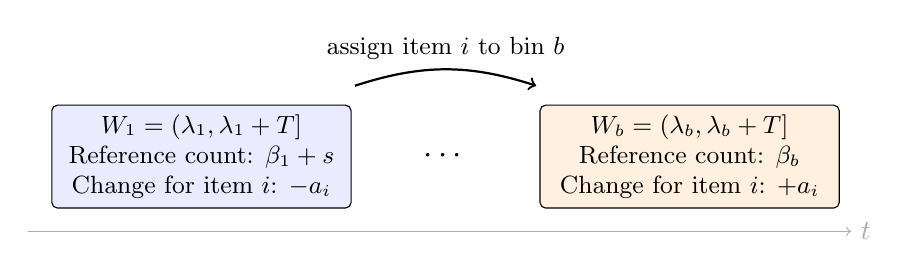
\begin{tikzpicture}[
  window/.style={draw,rounded corners=2pt,minimum width=3.8cm,
                 minimum height=1.15cm,align=center,font=\small}
]
  \node[window,fill=blue!8] (windowone) at (0,0)
    {$W_1=(\lambda_1,\lambda_1+T]$\\
     Reference count: $\beta_1+s$\\
     Change for item $i$: $-a_i$};
  \node[font=\large] at (3.1,0) {$\cdots$};
  \node[window,fill=orange!12] (windowb) at (6.2,0)
    {$W_b=(\lambda_b,\lambda_b+T]$\\
     Reference count: $\beta_b$\\
     Change for item $i$: $+a_i$};
  \draw[->,thick] (1.95,0.9) to[bend left=18]
    node[above,font=\small] {assign item $i$ to bin $b$}
    (4.25,0.9);
  \draw[->,gray!65] (-2.2,-0.95)--(8.25,-0.95)
    node[right] {$t$};
\end{tikzpicture}
\caption{Relative to the reference matching, assigning one item of
size $a_i$ from bin 1 to bin $b$ removes $a_i$ from the first
histogram window and adds $a_i$ to window $b$; intermediate windows
are unchanged. Superposing the item transfers gives
$N(t)=\beta_j+L_j$ throughout window
$W_j=(\lambda_j,\lambda_j+T]$.}
\label{fig:hardness-window-transfer}
\end{figure}

\subsection{Expected depth: an exact matching formula}

The expected-depth reduction needs no clouds. Each nonzero
hypothesis is one path vertex or one isolated vertex, and every
query isolates either a singleton or an adjacent pair.
The combinatorial choice is still a matching, but its objective
depends on how the resulting pairs are ordered.

For a finite positive weight vector $z$, keeping repeated values
as distinct entries, define the \emph{weighted completion sum} by
\[
 \mathcal C(z)=\sum_{j=1}^{|z|}jz_{(j)},
 \qquad z_{(1)}\ge\cdots\ge z_{(|z|)}.
\]
It equals the sum of the individual weights plus the smaller
weight for each unordered pair of entries: in decreasing order,
an earlier entry delays a later entry by one. Thus concatenating
vectors $u,v$ adds the cross contribution
$\sum_{i,j}\min\{u_i,v_j\}$.
Equivalently,
if $h_z(t)=|\{j:z_j\ge t\}|$, then
\begin{equation}\label{eq:completion-histogram}
 \mathcal C(z)=\int_0^\infty
                 \frac{h_z(t)(h_z(t)+1)}2\,dt.
\end{equation}
At height $t$, the first $h_z(t)$ ranks contribute
$1+\cdots+h_z(t)$; integrating those contributions proves the identity.

The completion sum becomes a tree objective once first-hit groups
are identified with a matching. This correspondence must hold for
arbitrary adaptive trees as well as for the sorted constructions.

\begin{lemma}[Exact singleton/pair formula]\label{lem:pair-invoice}
Consider a \emph{linear forest}, meaning a disjoint union of paths
(isolated vertices are allowed), with vertices $1,\ldots,N$ ordered
component by component. Represent them and a distinguished hypothesis by
$(i,i^2)$, $0\le i\le N$. Supply $I_{i,i}$ for each nonzero vertex
and $I_{i,i+1}$ for each forest edge.
Give the distinguished hypothesis weight $\omega_0>0$ and the
others positive weights $\omega_v$.
For a matching $\mathcal M$, let $J(\mathcal M)$ be the vector
containing mass
$\omega_u+\omega_v$ for each matched pair and $\omega_v$ for each
unmatched vertex, retaining multiplicities when masses coincide.
The optimal unnormalized expected depth is
\begin{equation}\label{eq:pair-invoice}
 \min_{\mathcal M}
 \left\{\omega_0(N-|\mathcal M|)
       +\mathcal C(J(\mathcal M))
       +\sum_{\{u,v\}\in\mathcal M}(\omega_u+\omega_v)\right\}.
\end{equation}
If $\omega_0>N\sum_{v>0}\omega_v$, an optimal matching in this
formula has maximum cardinality.
\end{lemma}
\begin{proofstrategy}
Read any tree from the distinguished all-miss spine: its disjoint
first-hit pairs form a matching. Then sort the group masses; adjacent
exchanges minimize first-cover cost. A sufficiently heavy distinguished
point forces maximum cardinality before any other cost matters.
\end{proofstrategy}
\begin{proof}
We first establish the invoice in both directions: extract its
terms from any adaptive tree, and realize them for any matching.
The distinguished-weight condition is a separate restriction applied
afterward.

\begin{claim}[First-hit groups attain the matching cost]
\label{clm:pair-invoice-attainable}
The spine contributes one query per singleton or matched pair, and
only a pair requires an extra local query.
\end{claim}
\begin{proof}
Follow hypothesis $0$, which misses every supplied membership query.
The hypotheses first covered together are disjoint singletons
or adjacent pairs. The pairs form a matching $\mathcal M$,
and the spine has $N-|\mathcal M|$ queries.
A pair's hit branch requires exactly one additional query;
a singleton branch requires none.
This gives the first and third terms of \eqref{eq:pair-invoice}.

For the first-cover term, suppose masses $a<b$ occupy consecutive
positions $j,j+1$. Their contribution is
$ja+(j+1)b$ in that order and $jb+(j+1)a$ after swapping, a decrease
of $b-a$. Repeated exchanges show that nonincreasing mass is optimal.
Every such ordering is executable: query the selected pairs
and the singleton tests for the unmatched vertices in that order.
The groups are disjoint, so each query's hit branch exits only
to its own group. This proves the
formula both as a lower bound on arbitrary trees and as an
attainable value for each matching.
\end{proof}

The exact invoice still permits matchings of different sizes. Giving
the distinguished point enough weight makes its spine length decisive,
so later gadget calculations need consider only maximum matchings.

\begin{claim}[The distinguished weight forces maximum cardinality]
\label{clm:pair-invoice-cardinality}
Under the stated dominance condition, minimizing its depth is the
first objective.
\end{claim}
\begin{proof}

Every proper complete tree has depth at most $N$, so the total
weighted depth of all nonzero hypotheses is at most
$N\sum_{v>0}\omega_v$. One additional query on hypothesis $0$'s
path outweighs this entire budget under the stated inequality.
An optimal tree must consequently minimize that path's length,
which means choosing a maximum-cardinality matching.
\end{proof}
\end{proof}

\subsection{Expected depth: bin loads become a quadratic penalty}

\begin{theorem}[Strong NP-completeness of expected depth]
\label{thm:strong-average}
Given supplied binary lines, strictly positive integer hypothesis
weights bounded by a fixed polynomial in $n$, and a rational threshold,
deciding the optimal expected depth is strongly NP-complete.
This holds for $\HH=\{(i,i^2):0\le i<n\}$, $O(n)$ integer-coefficient
lines, and negative answer classes of size at most two.
\end{theorem}

\begin{proofstrategy}
\begin{enumerate}
\item Use the exact matching cost formula and a heavy distinguished point
to normalize the optimum to one unmatched even vertex per item.
\item Pair-mass histograms encode bin loads. Integrating their tail
counts produces a quadratic load penalty and an unwanted linear term.
\item Tiny, ordered boundary-weight adjustments cancel that linear
term. Medium-weight isolated vertices exclude internal choices, and
scale separation makes rounding smaller than a unit imbalance.
\end{enumerate}
\end{proofstrategy}

\subsubsection{Construction and supporting propositions}

Let $q=2s(p-1)$ be the total matching size and define the reference
bin counts
\[
 \beta_1=q-s,\qquad \beta_b=2s(p-b)\quad(2\le b\le p).
\]
Take an isolated-vertex count $r$, an even window width $V$, and bin
levels $\lambda_b$ from Section~\ref{sec:average-hardness-calibration}.
The $r$ isolated vertices have weight $Z=V/2$. To cancel the bin
linear term, define
\[
 \begin{aligned}
 t_i&=q+r+m-i,&
 \delta_{ib}&=\left\lfloor\frac{V(\beta_1-\beta_b)a_i}{t_i}\right\rfloor,\\
 D&=\max_{i,b}\delta_{ib},& A_i&=1+(2D+1)i.
 \end{aligned}
\]
Here $t_i$ will be the exact coefficient of unmatched item $i$;
$A_i$ fixes the unmatched-weight order, and $\delta_{ib}$ is its small
bin-dependent correction. Since
$\beta_1-\beta_b=(2b-3)s>0$ for $b\ge2$, all corrections are
nonnegative and $\delta_{i1}=0$.

For item $i$, form an odd path
\[
 E_{i0},\,B_{i1},\,E_{i1},\,\ldots,\,
 B_{is_i},\,E_{is_i},\qquad s_i=2a_i(p-1),
\]
where each displayed symbol also denotes that vertex's weight.
First define unperturbed even weights
\[
 E^0_{ij}=
 \begin{cases}
 A_i,&j\equiv0\pmod{2a_i},\\
 A_i+V,&j\text{ odd},\\
 A_i+2V,&\text{otherwise}.
 \end{cases}
\]
Each consecutive difference is $+V$ or $-V$.
Between two boundary positions there are $2a_i$ steps,
of which $a_i$ go up and $a_i$ go down.
For $1\le j\le s_i$ let $b=\lceil j/(2a_i)\rceil$ and put
\[
 B_{ij}=
 \begin{cases}
 \lambda_b-E^0_{i,j-1},&E^0_{ij}-E^0_{i,j-1}=V,\\
 \lambda_{b+1}-E^0_{ij},&E^0_{ij}-E^0_{i,j-1}=-V.
 \end{cases}
\]
Finally set
$E_{i,2a_i(b-1)}=A_i+\delta_{ib}$ at each of the $p$ boundaries
and leave all other even weights unperturbed.
The odd weights do not change when this adjustment is made.

Add $r$ isolated forest vertices of weight $Z$.
The nonzero forest has $N=2q+m+r$ vertices, with maximum matching
size $q$. Let $P$ be the total weight of its item-path vertices,
$W=P+rZ$, and give hypothesis $0$ weight
$\omega_0=(N+1)W+1$.
Use precisely the lines of Lemma~\ref{lem:pair-invoice}.
Normalize the weights only after the construction.


Use $E_+=q\sum_{i,b}\delta_{ib}$ for the possible pair-mass
perturbation and $E_-=\sum_i(t_i-1)$ for the rounding loss.
Write $G$ for the minimum raw weighted cost for a fixed maximum
matching in Lemma~\ref{lem:pair-invoice}, $U=(U_1,\ldots,U_m)$ for
its unmatched item weights, and $z$ for its $q$ pair masses. Boundary choice $b_i$
assigns item $i$ to that bin, whose load is
$L_b=\sum_{i:b_i=b}a_i$.

The three weight classes serve different purposes: pair masses
carry the histogram, isolated vertices penalize internal choices, and
small boundary weights permit controlled corrections. Their separation
also fixes the orders used in the invoice.

\begin{proposition}[Separated scales and maximum-matching normalization]
\label{prop:average-normalization}
All weights are positive. Every pair mass exceeds $Z$ and every
unmatched item weight; boundary weights are below $Z$ and ordered by
item index. The optimum uses a maximum-cardinality matching, and the
calibration ensures $E_++E_-<V$.
\end{proposition}

Once matching cardinality is fixed, the distinguished contribution
and several cross terms are constant. The remaining completion and
unmatched-vertex costs vary with the bin choices, so we record their
sum in the matching cost formula below.

\begin{proposition}[The matching-dependent invoice]
\label{prop:average-invoice}
\begin{equation}\label{eq:expected-remaining-invoice}
 G=G_{\mathrm{fix}}+\mathcal C(z)+\mathcal C(U)
       +(q-1)\sum_i U_i+r\sum_i\min\{U_i,Z\},
\end{equation}
where
\[
 G_{\mathrm{fix}}=
 \omega_0(q+m+r)+\frac{Zr(r+1)}2+qrZ+P.
\]
\end{proposition}

For boundary matchings, the same transfer idea now changes pair
masses. The completion integral converts their tail counts into a
quadratic load term and a linear term.

\begin{proposition}[Pair windows give a quadratic load identity]
\label{prop:average-windows}
Let $b_i$ be the bin chosen by item $i$ and
$L_b=\sum_{i:b_i=b}a_i$. Let $z^0$ be the unperturbed pair-mass
vector for these choices, and let $C_{\mathrm{ref}}$ be the
completion sum of the reference vector in which every item chooses
bin $1$. Then
\begin{equation}\label{eq:expected-bin-identity}
 \mathcal C(z^0)=C_{\mathrm{ref}}+
 V\left[\sum_b\beta_bL_b-\beta_1s+
             \frac{\sum_bL_b^2-s^2}{2}\right].
\end{equation}
\end{proposition}

A quadratic penalty favors balanced loads only after the bin-dependent
linear term is removed. The boundary corrections perform that
cancellation, and the error bounds preserve a strict threshold gap.

\begin{proposition}[Boundary corrections cancel the linear term]
\label{prop:average-boundary-gap}
For every boundary matching, there is an error $e$ with
$-E_-\le e\le E_+$ such that
\begin{equation}\label{eq:expected-quadratic-gap}
 G=G_{\mathrm{fix}}+\sum_i t_iA_i+C_{\mathrm{ref}}+
       \frac V2\left(\sum_bL_b^2-s^2\right)+e.
\end{equation}
Define the raw threshold
\begin{equation}\label{eq:expected-raw-threshold}
 k_0=G_{\mathrm{fix}}+\sum_i t_iA_i+C_{\mathrm{ref}}
              +\frac V2(pB^2-s^2),\qquad k=k_0+E_+.
\end{equation}
A boundary matching has $G\le k$ exactly when every bin load is $B$.
\end{proposition}

The quadratic calculation concerns boundary choices. Full soundness
also requires excluding internal unmatched vertices; the isolated
vertices provide that penalty without introducing nonpolynomial data.

\begin{proposition}[Internal choices are excluded; encoding is strong]
\label{prop:average-internal-encoding}
Every maximum matching with an internal unmatched even vertex has
$G>k$. The construction and its normalized threshold $k/\Omega$,
where $\Omega=\omega_0+W$, have polynomially bounded numerical data
and $O(n)$ supplied lines; a proper tree is a polynomial NP certificate.
\end{proposition}

\begin{proof}[Proof of Theorem~\ref{thm:strong-average}]
A source partition selects boundary choices of raw cost at most $k$
by Proposition~\ref{prop:average-boundary-gap}. Conversely,
Proposition~\ref{prop:average-normalization} reduces the optimum to
maximum matchings. Proposition~\ref{prop:average-internal-encoding}
excludes internal unmatched vertices, so every unmatched item position
chooses a boundary and hence a bin. Proposition~\ref{prop:average-boundary-gap}
shows that a qualifying matching has every bin load equal to $B$.
Because two source items sum to less than $B$ and four sum to more than
$B$, each such bin contains exactly three items; the chosen bins
therefore give a 3-partition. Normalizing divides both objective and
threshold by $\Omega$, while the encoding proposition supplies strong
hardness and NP membership, including arbitrary adaptive trees.
\end{proof}

\subsubsection{Technical proofs of the expected-depth propositions}

\begin{proofstrategy}
Compare the weight classes in turn: pair masses must dominate unmatched
and isolated weights, while boundary weights must stay below the
isolation threshold and retain their item order. These inequalities
activate the invoice lemma's maximum-cardinality criterion.
\end{proofstrategy}
\begin{proof}[Proof of Proposition~\ref{prop:average-normalization}]
The scale estimates verified in Section~\ref{sec:average-hardness-calibration}
are used here only to compare the three weight classes.
Every even weight is positive. By the first bound in
\eqref{eq:expected-scale-bounds}, $A_i+\delta_{ib}<V/100$, so
$A_i+2V<2.01V$ and every unmatched even weight is below $3V$.
For an upward step, the two possible pair masses are
$\lambda_b$ and $\lambda_b+V$; for a downward step they are
$\lambda_{b+1}+V$ and $\lambda_{b+1}$. Since
$\lambda_b\ge12V$ and $\lambda_{b+1}\ge14V$, all these masses are
at least $12V$. Boundary adjustments are nonnegative and can only
increase a matched pair's mass. The odd weights are also positive:
each is either $\lambda_b-E^0_{i,j-1}$ or
$\lambda_{b+1}-E^0_{ij}$, and every unperturbed even weight is
less than $2.01V$. Hence every pair mass exceeds $Z=V/2$ and every
unmatched even weight.
Boundary weights are below $Z$, and they increase strictly with the
item index: $A_{i+1}-(A_i+D)=D+1>0$. Finally,
$E_++E_-<V$ follows from the last two calibration bounds.
Here $\omega_0=(N+1)W+1>NW$, so the dominance condition of
Lemma~\ref{lem:pair-invoice} restricts the optimum to maximum
matchings. By Lemma~\ref{lem:odd-path}, each item then leaves
one even vertex unmatched.
\end{proof}

\begin{proof}[Proof of Proposition~\ref{prop:average-invoice}]
Split the completion sum into $z,U$, and the vector of $r$
isolated weights $Z$. Its within-vector terms are
$\mathcal C(z)$, $\mathcal C(U)$, and $Zr(r+1)/2$.
Proposition~\ref{prop:average-normalization} puts every pair mass
above every unmatched and isolated weight. Thus the minimum-weight
cross-term identity preceding \eqref{eq:completion-histogram} gives
cross terms
$q\sum_iU_i$ and $qrZ$. The unmatched/isolated cross term is
$r\sum_i\min\{U_i,Z\}$. Thus the total completion term is
\[
 \mathcal C(z)+\mathcal C(U)+\frac{Zr(r+1)}2
       +q\sum_iU_i+qrZ+r\sum_i\min\{U_i,Z\}.
\]
The item paths partition into matched vertices and the unmatched
vertices, so the extra local pair cost is $P-\sum_iU_i$.
The witness path has $N-q=q+m+r$ queries and costs
$\omega_0(q+m+r)$. Adding these terms replaces $q\sum_iU_i$
by $(q-1)\sum_iU_i$ and gives the displayed
$G_{\mathrm{fix}}$, proving the invoice.
\end{proof}

\begin{proof}[Proof of Proposition~\ref{prop:average-windows}]
We first determine the pair-mass histogram for each boundary choice,
then integrate it. This separates the local matching calculation
from the algebra that produces the quadratic objective.

\begin{claim}[Boundary movement transfers pair masses between windows]
\label{clm:average-mass-transfer}
The pair-mass tail count in window $b$ is $\beta_b+L_b$, and it is unchanged outside the windows.
\end{claim}
\begin{proof}
By Lemma~\ref{lem:odd-path}, unmatching boundary $2a_i(b-1)$
fixes all left and right pairs and assigns item $i$ to bin $b$.
Temporarily omit the boundary perturbations and denote the
resulting pair-mass vector by $z^0$.
For an upward step in segment $b$, pairing its odd vertex
to the even vertex on the left gives mass $\lambda_b$,
while pairing right gives $\lambda_b+V$.
For a downward step, those masses are
$\lambda_{b+1}+V$ and $\lambda_{b+1}$.
Moving the unmatched vertex across a whole segment consequently
changes the pair-mass histogram by
\[
 -a_i\mathbf1_{(\lambda_b,\lambda_b+V]}+
  a_i\mathbf1_{(\lambda_{b+1},\lambda_{b+1}+V]}.
\]
There are exactly $a_i$ steps of each type.
Write $W_j=(\lambda_j,\lambda_j+V]$. Moving an item from
boundary 1 to boundary $b_i$ adds
\[
 a_i\sum_{j=1}^{b_i-1}
       (-\mathbf1_{W_j}+\mathbf1_{W_{j+1}})
 =-a_i\mathbf1_{W_1}+a_i\mathbf1_{W_{b_i}}.
\]
For $b_i=1$ this is zero; otherwise each intermediate indicator
cancels. This is the same telescoping mechanism as in the height
construction.
In the reference matching, all odd vertices are paired to their
right. Segment $b$ contributes $s$ masses $\lambda_b+V$ and
$s$ masses $\lambda_{b+1}$ after summing over items.
For a threshold $t$ in window $b$, where
$\lambda_b<t\le\lambda_b+V$, a segment $c<b$ contributes no mass:
its larger mass is $\lambda_{c+1}\le\lambda_b<t$. Every segment
$c\ge b$ contributes both batches, since
$\lambda_c+V\ge\lambda_b+V\ge t$ and
$\lambda_{c+1}>\lambda_b+V$. Therefore, when $b\ge2$, the
$p-b$ segments $c=b,\ldots,p-1$ contribute $2s(p-b)=\beta_b$
masses in total. In the first window all $p-1$ segments contribute,
so the reference count is $q=2s(p-1)=\beta_1+s$.
Assigning items according to loads $L_b$
changes the tail count throughout window $b$ to
$\beta_b+L_b$: the first window loses $s-L_1$ pair masses from its
reference count $q$, while each later window gains $L_b$.
Outside these disjoint windows the tail histogram is unchanged.
\end{proof}
The histogram now depends on the matching only through bin loads.
Integrating the triangular count polynomial reveals both the desired
imbalance penalty and the linear term that the next proposition
must cancel.

\begin{claim}[Integrating the tail counts yields the quadratic term]
\label{clm:average-integrated-windows}
The triangular histogram formula gives \eqref{eq:expected-bin-identity}.
\end{claim}
\begin{proof}
Let $C_{\mathrm{ref}}$ be the completion sum of the unperturbed
pair masses when every first boundary is unmatched. It is explicitly
computable by sorting those $q$ masses.
Let $f(h)=h(h+1)/2$. Direct expansion gives
\[
 f(\beta_b+L_b)-f(\beta_b)
 =\frac{2\beta_bL_b+L_b^2+L_b}{2}
 =\beta_bL_b+\frac{L_b^2+L_b}{2}.
\]
By Claim~\ref{clm:average-mass-transfer}, all windows have width
$V$ and the histogram outside them is unchanged. Therefore
\eqref{eq:completion-histogram} reduces the difference of completion
sums to those windows. Subtracting the reference loads $(s,0,\ldots,0)$
therefore gives
\begin{align*}
 \mathcal C(z^0)-C_{\mathrm{ref}}
 &=V\left[\sum_b\left(\beta_bL_b+
                    \frac{L_b^2+L_b}{2}\right)
               -\beta_1s-\frac{s^2+s}{2}\right]\\
 &=V\left[\sum_b\beta_bL_b-\beta_1s
        +\frac{\sum_bL_b^2-s^2}{2}
        +\frac{\sum_bL_b-s}{2}\right]\\
 &=V\left[\sum_b\beta_bL_b-\beta_1s
        +\frac{\sum_bL_b^2-s^2}{2}\right].
\end{align*}
The second equality separates the quadratic and linear load terms;
the last uses $\sum_bL_b=s$ to cancel the remaining unweighted
linear term. This proves the stated
identity and identifies the unwanted linear term that remains
alongside the useful quadratic term.
\end{proof}
\end{proof}

\begin{proof}[Proof of Proposition~\ref{prop:average-boundary-gap}]
The corrections affect two parts of the invoice. We bound their
incidental effect on pair completion cost, compute their intended
unmatched contribution, and finally compare the error with an
integral load imbalance.

\begin{claim}[Pair perturbations change completion cost by at most $E_+$]
\label{clm:average-pair-perturbation}
The increase is nonnegative and at most $q\sum_{i,b}\delta_{ib}$.
\end{claim}
\begin{proof}
Boundary perturbations increase pair masses by at most the total
added boundary weight. For a vector $z$ of $q$ pair masses,
$\mathcal C(z)=\min_\sigma\sum_{j=1}^q jz_{\sigma(j)}$, by the
adjacent-swap ordering argument in Lemma~\ref{lem:pair-invoice}.
Write the new vector as $z+d$ with $d_j\ge0$ and
$\Delta=\sum_jd_j$. Every ordering's weighted sum is nondecreasing,
so taking the minimum gives $\mathcal C(z+d)\ge\mathcal C(z)$.
If $\sigma$ minimizes the old vector, then
\[
 \mathcal C(z+d)
 \le\sum_{j=1}^q j(z_{\sigma(j)}+d_{\sigma(j)})
 \le\mathcal C(z)+q\sum_jd_j
 =\mathcal C(z)+q\Delta.
\]
The first inequality evaluates the new optimum in the old minimizing
order, while the second bounds each added mass's rank by $q$.
Thus a change in the sorted order cannot invalidate the perturbation
estimate.
A perturbed boundary vertex belongs to at most one matched pair,
so the total pair-mass increase is at most the sum of all boundary
corrections, $\Delta\le\sum_{i,b}\delta_{ib}$. Denote the pair
completion increase by $e_{\rm pair}$; the inequalities give
$0\le e_{\rm pair}\le E_+$.
\end{proof}
Pair completion may reorder after perturbation, which is why its
change was bounded separately. The unmatched weights keep their fixed
order, giving an exact coefficient for each correction and the
intended cancellation.

\begin{claim}[The unmatched ranks cancel the unwanted bin linear term]
\label{clm:average-linear-cancellation}
The boundary cost is \eqref{eq:expected-quadratic-gap} with $-E_-\le e\le E_+$.
\end{claim}
\begin{proof}
Proposition~\ref{prop:average-normalization} puts all boundary
unmatched weights below $Z$ and fixes their decreasing item order. Indeed,
$A_{i+1}-(A_i+D)=D+1>0$, so even the largest perturbation of item
$i$ leaves it below the unperturbed weight of item $i+1$.
Thus their terms in \eqref{eq:expected-remaining-invoice} are
$\sum_i t_i(A_i+\delta_{ib_i})$.
Indeed, item $i$ has rank $m-i+1$ in $\mathcal C(U)$, plus
coefficient $q-1+r$ from the other terms, giving $t_i=q+r+m-i$.
The floor definition gives
\[
 -E_-\le
 \sum_i t_i\delta_{ib_i}
       -V\sum_i(\beta_1-\beta_{b_i})a_i
 \le0.
\]
For each item, the difference is minus the remainder when the
integer $V(\beta_1-\beta_{b_i})a_i$ is divided by $t_i$; its
magnitude is therefore at most $t_i-1$.
Write
$e_{\rm floor}=\sum_i t_i\delta_{ib_i}
                 -V\sum_i(\beta_1-\beta_{b_i})a_i$.
The remainder calculation gives $-E_-\le e_{\rm floor}\le0$.
Grouping the intended correction by chosen bin gives
\[
 V\sum_i(\beta_1-\beta_{b_i})a_i
 =V\beta_1s-V\sum_b\beta_bL_b.
\]
In the invoice the unmatched terms are
$\sum_i t_iA_i+\sum_i t_i\delta_{ib_i}$, while the pair
completion term equals the window expression plus $e_{\rm pair}$.
Substituting \eqref{eq:expected-bin-identity} for the unperturbed
pair completion term and Claim~\ref{clm:average-pair-perturbation}
for its change gives
\begin{align*}
 G={}&G_{\mathrm{fix}}+\sum_i t_iA_i+C_{\mathrm{ref}}\\
 &+V\left[\sum_b\beta_bL_b-\beta_1s
              +\frac{\sum_bL_b^2-s^2}{2}\right]\\
 &+V\beta_1s-V\sum_b\beta_bL_b
       +e_{\rm floor}+e_{\rm pair}\\
 ={}&G_{\mathrm{fix}}+\sum_i t_iA_i+C_{\mathrm{ref}}
       +\frac V2(\sum_bL_b^2-s^2)+e.
\end{align*}
Here $e=e_{\rm floor}+e_{\rm pair}$ satisfies
$-E_-\le e\le E_+$, since the first summand is nonpositive
and the second is nonnegative with the respective bounds.
\end{proof}
After cancellation, the only matching-dependent term of substantial
size is the quadratic load penalty. Integral loads give a minimum
positive imbalance, and scale separation prevents the bounded errors
from hiding it.

\begin{claim}[An unbalanced integral load costs more than the error budget]
\label{clm:average-imbalance-gap}
The threshold $k$ is met exactly when all loads equal $B$.
\end{claim}
\begin{proofstrategy}
Center each load at $B$ and expand the sum of squared deviations; the
fixed total load removes the linear term. A valid partition then has
zero penalty, whereas any other integral zero-sum deviation has penalty
at least $V$. Finally compare that gap with the two calibrated error
bounds.
\end{proofstrategy}
\begin{proof}
Write $\Delta_b=L_b-B$ for the deviation of bin $b$ from its target load.
Since the loads total $pB$, these deviations sum to zero. Expanding each
square, then using that total-load identity, gives
\begin{align*}
 \sum_b(L_b-B)^2
 &=\sum_bL_b^2-2B\sum_bL_b+pB^2
       &&\text{by termwise expansion and summation}\\
 &=\sum_bL_b^2-pB^2
       &&\text{since }\sum_bL_b=pB.
\end{align*}
Substituting this identity into
Claim~\ref{clm:average-linear-cancellation} and the definition of $k_0$
rewrites the corrected invoice as
\[
 G=k_0+\frac V2\sum_b\Delta_b^2+e,
 \qquad -E_-\le e\le E_+.
\]
If the source instance has a valid partition, every load equals $B$,
so each $\Delta_b=0$. The invoice is then $G=k_0+e\le k_0+E_+=k$.

Conversely, suppose the loads are not all $B$. The deviations are
integers, sum to zero, and are not all zero. They must therefore include
both a positive and a negative entry: if all were nonnegative or all
nonpositive, a zero sum would force every entry to vanish. Each nonzero
integer has square at least one, so
\[
 \sum_b\Delta_b^2\ge 1^2+(-1)^2=2.
\]
It follows that the quadratic penalty is at least
$(V/2)\cdot2=V$. Together with $e\ge-E_-$, this gives
$G\ge k_0+V-E_-$. Finally, the two bounds in
\eqref{eq:expected-scale-bounds} imply
\[
 V-E_->\frac{1999}{2000}V
       >\frac{1}{1000}V\ge E_+.
\]
The first strict inequality uses $E_-<V/2000$; the middle inequality
follows from $V>0$ and $1999/2000>1/1000$; the last is the stated bound
on $E_+$. Hence $G>k_0+E_+=k$, so an unbalanced load cannot meet the
threshold.
\end{proof}
\end{proof}

\begin{proof}[Proof of Proposition~\ref{prop:average-internal-encoding}]
We complete soundness before checking encoding. An internal unmatched
vertex is heavier than the isolated vertices, so its repeated cross
interactions create a penalty exceeding the entire boundary threshold
allowance.

\begin{claim}[The isolated-vertex penalty excludes every internal choice]
\label{clm:average-internal-penalty}
An internal unmatched even vertex makes the raw invoice exceed $k$.
\end{claim}
\begin{proofstrategy}
Lower-bound the isolated-vertex cross term when an internal vertex is
unmatched, and upper-bound the threshold using the balanced-load
formula. The calibration makes the former penalty larger than all
remaining threshold terms.
\end{proofstrategy}
\begin{proof}
The preceding calculation proves soundness for boundary choices.
It remains to rule out a maximum matching that leaves an internal even
vertex unmatched. By Lemma~\ref{lem:odd-path}, every maximum matching
leaves one even vertex unmatched on each item path. If item $i$ uses a
boundary, its unmatched weight is $U_i=A_i+\delta_{ib_i}$ for some bin
$b_i$, with $\delta_{ib_i}\ge0$. An internal choice instead has weight
$A_i+V$ or $A_i+2V$. Thus every unmatched weight satisfies
$U_i\ge A_i$, while the internal choice at item $i_*$ has $U_{i_*}>Z$
because $V=2Z$. Since $\delta_{i1}=0$, the scale bound
\eqref{eq:expected-scale-bounds} gives
$A_i=A_i+\delta_{i1}<V/100<V/2=Z$. Consequently
$\min\{U_i,Z\}\ge A_i$ for every item, and
$\min\{U_{i_*},Z\}=Z$. Therefore
\[
 \sum_i\min\{U_i,Z\}
 =Z+\sum_{i\ne i_*}\min\{U_i,Z\}
 \ge Z+\sum_{i\ne i_*}A_i
 =\sum_iA_i+Z-A_{i_*}
 \ge\sum_iA_i+Z-\max_iA_i.
\]
The other terms in the matching-dependent invoice
\eqref{eq:expected-remaining-invoice} are nonnegative. Indeed,
$\mathcal C(z)$ and $\mathcal C(U)$ are positive completion sums, and
$q=2s(p-1)\ge2$ because $p\ge2$ and $s=pB\ge1$; hence
$(q-1)\sum_iU_i\ge0$ by positivity of the unmatched weights. Since
$r>0$ as well, substituting the preceding lower bound into the
isolated-vertex term and retaining the other nonnegative terms gives
\[
 G\ge G_{\mathrm{fix}}+r\sum_i A_i+
                   r\bigl(Z-\max_i A_i\bigr).
\]
We compare this with the boundary threshold from
Proposition~\ref{prop:average-boundary-gap}, whose threshold definition
is recorded in \eqref{eq:expected-raw-threshold}. Since $s=pB$ and
$p\ge2$,
\[
 pB^2-s^2=pB^2-p^2B^2=-p(p-1)B^2\le0.
\]
Thus the quadratic reference term in $k_0$ is nonpositive and may be
dropped for an upper bound. Moreover, from $t_i=q+r+m-i$ we obtain
\[
 \sum_i t_iA_i
 =r\sum_iA_i+\sum_i(q+m-i)A_i
 \le r\sum_iA_i+(q+m)\sum_iA_i,
\]
because $q+m-i\le q+m$ and every $A_i$ is positive. Substituting this
bound into the threshold formula gives
\[
 k\le G_{\mathrm{fix}}+r\sum_i A_i+
           C_{\mathrm{ref}}+(q+m)\sum_i A_i+E_+.
\]
Each reference pair mass is one of $\lambda_b$ or $\lambda_b+V$.
Because $\lambda_b=(10+2b)V$ increases with $b$, every such mass is at
most $\lambda_p+V=(11+2p)V$. By the definition of the weighted
completion sum, these $q$ masses receive ranks $1,\ldots,q$; hence
\[
 C_{\mathrm{ref}}
 \le(11+2p)V\frac{q(q+1)}2
 <(p+6)(q+1)^2V.
\]
The first inequality bounds every reference mass by its largest
level and sums the ranks $1,\ldots,q$. For the strict step,
$(11+2p)/2=p+11/2<p+6$, and $q(q+1)<(q+1)^2$ because $q+1>0$.
Also, \eqref{eq:expected-scale-bounds} with $\delta_{i1}=0$ gives
$A_i<V/100$ for every $i$, so $\sum_iA_i<mV/100$; the same scale
bounds give $E_+\le V/1000$. Set $X=(q+m+1)^2V$. Since
$q+1\le q+m+1$ and $m\le q+m+1$, we have
$(q+1)^2V\le X$ and $(q+m)mV\le X$. Also $q+m+1\ge1$, so
$V/1000\le X/1000$. Therefore
\begin{align*}
 C_{\mathrm{ref}}+(q+m)\sum_iA_i+E_+
 &<(p+6)X+\frac X{100}+\frac X{1000}\\
 &<(p+8)X.
\end{align*}
The last strict inequality follows from
$p+6+1/100+1/1000<p+8$.
The calibration also gives the factors in the penalty explicitly:
$Z=V/2$ and $\max_iA_i<V/100$, so
$Z-\max_iA_i>V/2-V/100=49V/100>V/3$. Its definition of $r$ gives
$r>1000(p+10)(q+m+1)^2$, since the remaining summands in the
brackets are positive. Multiplying these positive bounds gives
\[
 r(Z-\max_iA_i)>
 \frac{1000}{3}(p+10)(q+m+1)^2V
 >(p+8)(q+m+1)^2V,
\]
where the final inequality follows from
$1000(p+10)>3(p+8)$. Thus the internal-choice lower bound exceeds
the threshold upper bound. These bounds share the term
$G_{\mathrm{fix}}+r\sum_iA_i$; after subtracting it, the penalty
remainder is strictly larger than the threshold remainder, so $G>k$.
\end{proof}
The penalty and error margins must be attainable with polynomial
scales. The final size calculation verifies this and gives the
certificate bound needed for strong NP-completeness.

\begin{claim}[The reduction has polynomial numerical data and certificates]
The normalized instance establishes strong hardness with polynomially
bounded numerical data.
\end{claim}
\begin{proofstrategy}
Bound the unnormalized weights from the source-size parameters, then
bound their sum and the distinguished weight. These bounds control the
normalized rational input size; the proper-tree certificate has at
most $n-1$ internal nodes and is checked by simulating its supplied
queries.
\end{proofstrategy}
\begin{proof}
Normalize the positive weights by their total $\Omega$ and use
the expected-depth threshold $k/\Omega$.
The source restriction above gives $B=\operatorname{poly}(m)$ and
$a_{\max}<B/2$, while $p=m/3$. Hence $s=pB$, $q=2s(p-1)$,
$\beta_1=q-s$, and the calibrated value of $r$ are all polynomial in
$m$. The same then holds for $V$ and the bin levels $\lambda_b$. The
floor formula makes each $\delta_{ib}$ polynomially bounded, so its
maximum $D$, the boundary weights $A_i$, and the even and odd path
weights are polynomially bounded as well. Consequently $W$ and
$\omega_0=(N+1)W+1$ are polynomially bounded. Thus the forest, its
weights, and the $O(N)$ supplied lines are constructed in polynomial
time in the source input.
Write $n=N+1$. The forest has $N=2q+m+r$ vertices, so
$q,m,r\le N<n$. Moreover, $q=2s(p-1)$ with $s\ge1$ gives
$p\le q+1\le n$ and $s\le q/2<n$. Since $B=s/p\le s$,
$B<n$ as well. In the calibration formula for $r$, the factor
$\beta_1=q-s=s(2p-3)$ is at least one, and $qmp+2m+1\ge1$;
therefore its second summand alone gives $r\ge a_{\max}$. We have
thus bounded every source-size parameter by $n$. It follows that
$V=2000m(r+q+m+1)=O(n^2)$ and
$\lambda_b=(10+2b)V=O(n^3)$. Proposition~\ref{prop:average-normalization}
gives $A_i+\delta_{ib}<V/100$ and $E^0_{ij}<2.01V$. Every odd
weight is either $\lambda_b-E^0_{i,j-1}$ or
$\lambda_{b+1}-E^0_{ij}$. Since $\lambda_b\ge12V$, these weights
are positive; subtracting a positive even weight also places each
below its corresponding bin level, and hence below $\lambda_{b+1}$.
The same proposition bounds internal even weights by $3V$; isolated
weights equal $V/2$. Thus every nonzero weight is $O(n^3)$. There are
$O(n)$ vertices, so the total nonzero
weight $W=P+rZ$ is $O(n^4)$, and the distinguished weight
$\omega_0=(N+1)W+1$ is $O(n^5)$.

The parabola abscissae are at most $N$, their squares are $O(n^2)$,
and the singleton and pair lines $I_{a,b}$ have coefficients bounded
by $O(n^2)$. There are $N$ singleton queries and at most $N$
path-edge queries. A proper complete tree has $n-1$ internal nodes,
so evaluating its supplied answers and weighted depths takes polynomial
time. We next bound the threshold. Its distinguished term in
$G_{\mathrm{fix}}$ is $\omega_0(q+m+r)=O(n^6)$. The other terms have
smaller orders: $Zr(r+1)/2=O(n^4)$, $qrZ=O(n^4)$, and $P=O(n^4)$.
Therefore $G_{\mathrm{fix}}=O(n^6)$. The reference completion sum has
$q=O(n)$ pair masses. Each is at most $(11+2p)V=O(n^3)$, and its rank
is at most $q=O(n)$; summing these $O(n)$ contributions gives
$C_{\mathrm{ref}}=O(n^5)$. Also, $t_i=O(n)$ and $A_i<V/100=O(n^2)$,
so $\sum_i t_iA_i=O(n^4)$. Since $s=pB$ and $p\ge2$,
\[
 \left|pB^2-s^2\right|=p(p-1)B^2
   =s^2\frac{p-1}{p}\le s^2.
\]
Therefore the magnitude of the quadratic threshold term is at most
$Vs^2/2=O(n^4)$.
Finally, $E_+\le V/1000=O(n^2)$. Applying
these estimates to each term in $k$ gives $|k|=O(n^6)$, while
$\Omega=W+\omega_0=O(n^5)$ and $\Omega\ge1$. Thus every normalized
prior has a polynomially bounded integer numerator and denominator,
as does $k/\Omega$. This establishes strong NP-completeness with
strictly positive, polynomially bounded hypothesis weights.
\end{proof}
\end{proof}

\subsubsection{Calibration of the expected-depth construction}
\label{sec:average-hardness-calibration}

The semantic quantities $q,\beta_b,t_i,L_b$ describe matchings and
bin loads. The following slack choices only separate their weight
scales; they are not additional source data.
\begin{parameterchoice}
With $a_{\max}=\max_i a_i$, choose
\[
 \begin{aligned}
 r&=1000\bigl[(p+10)(q+m+1)^2
             +(qmp+2m+1)\beta_1a_{\max}+1\bigr],\\
 V&=2000m(r+q+m+1),\qquad
 \lambda_b=(10+2b)V\quad(1\le b\le p).
 \end{aligned}
\]
These polynomial integers make $V$ even and give
\begin{equation}\label{eq:expected-scale-bounds}
 \max_{i,b}(A_i+\delta_{ib})<V/100,\qquad
 E_+\le V/1000,\qquad E_-<V/2000.
\end{equation}
In particular $E_++E_-<V$; a load imbalance cannot be hidden by
rounding or pair perturbation.
\end{parameterchoice}

Since $t_i=q+r+m-i\ge r$ and $0\le\beta_b\le\beta_1$,
the floor definition gives
$\delta_{ib}\le V\beta_1a_{\max}/r$ and hence the same bound
for $D$. The second term in $r$ makes
$r>1000(qmp+2m+1)\beta_1a_{\max}$. Therefore
\[
 E_+=q\sum_{i,b}\delta_{ib}
 \le qmpD
 <\frac{qmp}{1000(qmp+2m+1)}V<\frac V{1000}.
\]
The first inequality bounds each of the $mp$ corrections by $D$;
the next substitutes the strict lower bound on $r$ into the estimate
for $D$, and the last uses $qmp<qmp+2m+1$.
Similarly $(2m+1)D<V/1000$. The largest adjusted boundary weight
satisfies
\begin{align*}
 A_i+\delta_{ib}
 &\le1+(2D+1)m+D=(2m+1)D+m+1\\
 &<\frac V{1000}+\frac V{2000}<\frac V{100}.
\end{align*}
Here $m+1\le V/2000=m(r+q+m+1)$ because $m\ge1$ and
$r+q+m+1\ge m+1$. Also $t_i-1<r+q+m+1$, so
\[
 E_-=\sum_i(t_i-1)<m(r+q+m+1)=\frac V{2000}.
\]
In particular $E_++E_-<3V/2000<V$.

The boundary bound gives
$Z-\max_iA_i>V/2-V/100=49V/100>V/3$.
The first term of $r$ gives
$r/3\ge(1000/3)(p+10)(q+m+1)^2>(p+8)(q+m+1)^2$,
since $1000(p+10)>3(p+8)$. Together these bounds exclude internal
unmatched vertices: the boundary gap supplies the per-vertex penalty,
and the lower bound on $r$ makes that penalty dominate the adjustment
error. Both quantities remain polynomial in the restricted source data.

\section{Uniform expected-depth hardness}
\label{sec:uniform-hardness}

We transfer the weighted singleton/pair hardness instance to a uniform
prior by replacing each vertex of weight $w$ with a cloud of $w$
hypotheses. Private queries can occur anywhere in an adaptive tree,
so the key step is to move them off the distinguished spine while
preserving or reducing cost. This normalization exposes whole clouds
as matching groups and yields an exact identity: the cloud optimum is
the weighted optimum plus a computable internal-cloud cost. Here raw
uniform cost denotes the sum of leaf depths, before division by the
number of hypotheses.

\subsection{Exact cloud replacement: normalization before accounting}

\subsubsection{The construction}

Consider the weighted singleton/pair linear forest instance of
Lemma~\ref{lem:pair-invoice}, with vertices $0,1,\ldots,N$ and
positive integer weights $w_0,\ldots,w_N$. Vertex $0$ is
distinguished. Order the nonzero vertices along each path and
component by component, so every edge joins consecutive indices.
Here a cloud $C_i$ is the block of $w_i$ hypotheses representing
vertex $i$, its anchor is the point with offset $j=0$, and a private
query is one of the supplied lines that isolates a single nonanchor
point. The singleton and pair queries represent, respectively, a
vertex and an edge of the weighted forest. The invoice notation
$J(\mathcal M)$ and $\mathcal C(J(\mathcal M))$ is as in
Lemma~\ref{lem:pair-invoice}; it records the weighted instance left
after choosing the matching $\mathcal M$ of pair queries.
Choose the cloud spacing $Q$ by the final calibration below and define
\[
 n=\sum_{i=0}^N w_i,\qquad
 C_i=\{(Qi+j,(Qi+j)^2):0\le j<w_i\}.
\]
The point with $j=0$ is the anchor of cloud $C_i$.
For every nonzero vertex supply its whole-cloud singleton query;
for every linear forest edge supply its whole-cloud pair query.
For consecutive cloud indices $a,\ldots,b$, these are the negative
answers of
\begin{equation}\label{eq:uniform-cloud-membership}
 4y-4Q(a+b)x+Q^2(2a-1)(2b+1)=0.
\end{equation}
The value on the parabola factors as
$4(x-Q(a-\tfrac12))(x-Q(b+\tfrac12))$.
The product is negative exactly between its two roots. Cloud $c$ has
abscissae in $[Qc,Qc+w_c-1]$, with $w_c-1<Q/4$; hence every point
in clouds $a$ through $b$ lies strictly between the roots, while each
other cloud lies strictly outside. Since $a>0$, cloud $0$ is
excluded. Thus the negative answer selects exactly the designated
cloud or adjacent pair, and no point lies on the query line.

For every nonanchor point of abscissa $t$, including those of
cloud $0$, supply the private line
\[
 2y-4tx+2t^2-1=0.
\]
Its value on $(x,x^2)$ is $2(x-t)^2-1$; it is negative at $x=t$
and positive at every other integer abscissa, since then $|x-t|\ge1$.
It therefore isolates precisely that point, with no point on the line.
No private line is supplied for an anchor. All answers are strict
and binary. The whole-cloud singleton queries distinguish each
nonzero anchor from all other anchors and cloud $0$; the private
queries then separate every nonanchor from the anchor in its cloud.
Consequently the query family identifies every hypothesis. There are
$n=\sum_iw_i$ hypotheses, so the uniform prior gives each weight $1/n$.

Put
\begin{equation}\label{eq:uniform-cloud-offset}
 D(w)=\frac{(w-1)(w+2)}2,\qquad
 \Delta=\sum_{i=0}^N D(w_i).
\end{equation}
Algorithm~\ref{alg:uniform-cloud-lift} gives the construction and
the threshold conversion.

\begin{algorithm}[H]
\caption{Uniform cloud replacement of a weighted linear forest instance}
\label{alg:uniform-cloud-lift}
\KwIn{Vertices $0,\ldots,N$ with each path in order, component by component,
positive integer weights $w_i$, and a raw weighted threshold $k$}
\KwOut{Supplied-line instance with uniform prior and threshold
$(k+\Delta)/n$}
$Q\gets4\max_i w_i$; $n\gets\sum_iw_i$;
$\HH\gets\varnothing$; $\LL\gets\varnothing$\;
\For{$i=0,\ldots,N$}{
  \For{$j=0,\ldots,w_i-1$}{
    $t\gets Qi+j$; add $(t,t^2)$ to $\HH$\;
    \If{$j>0$}{
      Add $2y-4tx+2t^2-1=0$ to $\LL$\;
    }
  }
}
For each $i>0$, add \eqref{eq:uniform-cloud-membership}
with $(a,b)=(i,i)$ to $\LL$\;
For each linear forest edge $\{i,i+1\}$, add
\eqref{eq:uniform-cloud-membership} with $(a,b)=(i,i+1)$ to $\LL$\;
$\Delta\gets\sum_{i=0}^N(w_i-1)(w_i+2)/2$\;
\KwRet $(\HH,\LL)$, prior $1/n$, and threshold $(k+\Delta)/n$\;
\end{algorithm}

\begin{theorem}[Exact uniform cloud transfer]\label{thm:uniform-cloud-transfer}
Let $\OPT_{\mathrm{raw}}^{\mathrm{weighted}}$ be the minimum
raw weighted cost of the singleton/pair linear forest instance.
For its uniform cloud replacement,
\begin{equation}\label{eq:uniform-cloud-transfer}
 n\OPT_{\mathrm E}^{\mathrm{cloud}}
   =\OPT_{\mathrm{raw}}^{\mathrm{weighted}}+\Delta.
\end{equation}
Equivalently, if $J(\mathcal M)$ has the pair and singleton masses
from Lemma~\ref{lem:pair-invoice}, the raw uniform optimum is
\[
 \Delta+\min_{\mathcal M}
 \left\{w_0(N-|\mathcal M|)
   +\mathcal C(J(\mathcal M))
   +\sum_{\{u,v\}\in\mathcal M}(w_u+w_v)\right\}.
\]
\end{theorem}

\begin{proofstrategy}
\begin{enumerate}
\item Rotate a private singleton past the next query. Equal point
weights make its one-unit depth increase no larger than the savings
on the opposite, nonempty answer branch.
\item Push all external private queries off the distinguished anchor's
spine and move its own private chain to the end. Every first-hit cloud
is then intact, so the first-hit pairs form a matching.
\item Sum exact one- and two-cloud local costs, then sort group sizes.
The result is the weighted matching cost plus the fixed offset
$\Delta$; the same construction attains it.
\end{enumerate}
\end{proofstrategy}

\subsubsection{Three supporting statements}

Uniform weights make one local exchange cost nonincreasing: delaying
an isolated point by one query saves a query for a nonempty opposite
branch. Since every point has the same weight, the exchange changes
the raw cost only through the depths immediately above the attached
subtrees; their internal costs cancel. This is the tool for
normalizing arbitrary trees.

\begin{lemma}[Uniform singleton rotation]\label{lem:uniform-singleton-rotation}
Suppose a proper identifying tree on a uniformly weighted state $S$
first asks a supplied query isolating $x\in S$, and the other child
first asks a query $r$ that is proper on $S\setminus\{x\}$.
These two queries can be exchanged, placing the singleton query
in the answer branch of $r$ containing $x$, without increasing
the raw cost.
\end{lemma}
Once clouds reach their first hit intact, their internal cost can
be accounted for exactly. We need both the single-cloud value and
a check that early private queries cannot improve a two-cloud exit.

\begin{lemma}[Local uniform cloud costs]\label{lem:uniform-cloud-local}
The optimal raw local cost on one intact cloud of size $w$ is
$D(w)$. On two intact clouds of sizes $u,v$, it is
\[
 D(u)+D(v)+u+v.
\]
\end{lemma}

The rotations must establish a global normal form before costs
are summed. External private queries leave the distinguished spine,
while its own private chain moves to the end, exposing whole-cloud
matching groups.

\begin{proposition}[A normalized matching spine]
\label{prop:uniform-cloud-spine}
An optimal uniform cloud tree can be chosen so that its distinguished
anchor's path first asks only whole-cloud queries, with every newly
hit cloud intact, and then asks only cloud-$0$ private queries.
The first-hit pairs form a matching $\mathcal M$. For this matching,
the best raw cost is
\[
 \Delta+w_0(N-|\mathcal M|)+\mathcal C(J(\mathcal M))
          +\sum_{\{u,v\}\in\mathcal M}(w_u+w_v).
\]
Every matching has a tree attaining this invoice.
\end{proposition}

\begin{proof}[Proof of Theorem~\ref{thm:uniform-cloud-transfer}]
Lemma~\ref{lem:uniform-singleton-rotation} permits the normalization
in Proposition~\ref{prop:uniform-cloud-spine} without increasing cost.
Lemma~\ref{lem:uniform-cloud-local} supplies its exact local offset.
Minimize the resulting invoice over matchings and apply
Lemma~\ref{lem:pair-invoice}. This gives
$\OPT_{\mathrm{raw}}^{\mathrm{cloud}}
=\OPT_{\mathrm{raw}}^{\mathrm{weighted}}+\Delta$.
Dividing by $n$ proves the displayed expected-depth identity.
\end{proof}

\subsubsection{Technical proofs of the supporting statements}

\begin{proofstrategy}
First, compare the two possible query orders by their per-state depth
changes; uniform weights make the singleton rotation nonincreasing.
Next, compute the forced private-chain cost for one cloud and use
induction to show that a whole-cloud separator is optimal for two.
Finally, apply those rotations to normalize the distinguished path,
then sum each first-hit group's local cost and order the groups by
decreasing mass. This yields the matching cost formula and its attaining
construction.
\end{proofstrategy}

\begin{proof}[Proof of Lemma~\ref{lem:uniform-singleton-rotation}]
Let $A,B$ be the two nonempty answer classes of $r$ on
$S\setminus\{x\}$, and choose their names so that $x$ has the
answer of $A$. In the original tree, $x$ has relative depth one
and every hypothesis in $A\cup B$ passes through both queries.
Ask $r$ first, put the private singleton query in its
$A\cup\{x\}$ branch, and attach the original subtrees on $A$ and
$B$. Originally $x$ has relative depth one and points of $A$ and $B$
have relative depth two before their attached subtrees. Afterwards
$x$ has relative depth two, the points of $A$ still have depth two,
and the points of $B$ have depth one before their unchanged subtrees.
Thus the raw cost change is
\[
 (2-1)+|A|(2-2)+|B|(1-2)=1-|B|\le0,
\]
because $B$ is nonempty. The resulting queries are
proper and are members of the original supplied family.
\end{proof}

If the opposite class $B$ has one point, the rotation has zero cost;
if it has more than one, the cost decreases. The lemma concerns
equal weights, so we use the rotation only when every point contributes
the same unit cost at each level.

\begin{proof}[Proof of Lemma~\ref{lem:uniform-cloud-local}]
We first compute the forced private-chain cost within one cloud.
For two clouds, we then compare separating them immediately with
every possible private-first choice; this verifies the offset without
assuming a local normal form.

\begin{claim}[A single cloud forces a private chain]
\label{clm:uniform-cloud-chain}
Its raw local cost is $D(w)$, including zero cost when $w=1$.
\end{claim}
\begin{proof}
Within one cloud, every whole-cloud query is constant, and every
nonconstant query isolates one of its nonanchors. The only possible
proper code is a chain: every private query has a singleton outcome,
and the other outcome retains the anchor and all points not yet
isolated. Thus the nonanchors exit at depths $1,\ldots,w-1$, and
the anchor exits at depth $w-1$. The sum of depths is
$1+2+\cdots+(w-1)+(w-1)$. For $w\ge2$,
\[
 \sum_{j=1}^{w-1}j+(w-1)
 =\frac{w(w-1)}2+(w-1)
 =\frac{(w-1)(w+2)}2=D(w).
\]
For $w=1$ there is no query and both the sum and $D(1)$ are zero.

\end{proof}
Separating the clouds gives the proposed cost directly. The remaining
question is whether isolating a private point first could save more;
induction accounts for the delay imposed on the other cloud.

\begin{claim}[A whole-cloud separator is optimal on two clouds]
\label{clm:uniform-cloud-separator}
Private-first choices cannot beat $D(u)+D(v)+u+v$.
\end{claim}
\begin{proof}
On two clouds a nonconstant whole-cloud query separates the
clouds. Its root query is traversed by all $u+v$ points, after which
the clouds cost $D(u)+D(v)$; this attains the displayed formula.
Every other nonconstant query isolates one nonanchor. Induct on
$u+v$, with the whole-cloud separator available at every induction
state.
If a private point of the $u$ cloud is queried first, the
remaining two-cloud state has sizes $u-1,v$ and still has its
anchors and whole-cloud separator. Using induction, this choice
costs
\[
 u+v+D(u-1)+D(v)+(u-1)+v.
\]
A private point exists in this cloud only if $u\ge2$. The
single-cloud formula of Claim~\ref{clm:uniform-cloud-chain} gives
\[
 D(u)-D(u-1)
 =\frac{(u-1)(u+2)-(u-2)(u+1)}2=u.
\]
Subtracting the proposed separator cost from the private-first cost
therefore gives
\begin{align*}
 &[u+v+D(u-1)+D(v)+(u-1)+v]
       -[D(u)+D(v)+u+v]\\
 &\qquad=D(u-1)-D(u)+(u-1)+v
          =-u+(u-1)+v=v-1\ge0.
\end{align*}
The second equality substitutes $D(u)-D(u-1)=u$, and the final
inequality uses the presence of the other cloud, namely $v\ge1$.
Thus any saving on the queried cloud is paid for by delaying the
other cloud's points.
For a private point in the other cloud, the identical calculation
with $u,v$ interchanged gives $u-1\ge0$. The base case $u=v=1$ has raw cost two.
When one size is one it has no private point, and the same
induction applies to the other cloud. Queries selecting other
clouds are constant or separate these two whole clouds, so the
argument covers the entire supplied family.
\end{proof}
\end{proof}


\begin{proof}[Proof of Proposition~\ref{prop:uniform-cloud-spine}]
The two normalization steps have different destinations. A nonzero
cloud's private query should leave the distinguished path at its
whole-cloud hit; a cloud-$0$ private query stays on that path but
moves behind its whole-cloud queries.

\begin{claim}[External private queries can be pushed off the spine]
\label{clm:uniform-cloud-external-private}
No nonzero cloud needs to lose a private point before its first whole-cloud hit.
\end{claim}
\begin{proof}
Start with a proper optimal uniform tree and follow the anchor
of cloud $0$. Suppose a private query for a nonanchor $x$ of a
nonzero cloud occurs on this path. Its own cloud anchor is still
on the path: $x$ agrees with its anchor on every whole-cloud query,
and private queries never remove an anchor.
At each step, let $r$ be the next query on the anchor-$0$ path.
The private query isolates $x$, so the anchor-$0$ path continues in
the other child; the state reaching $r$ is precisely that non-$x$
answer class. Since $r$ is proper on $S\setminus\{x\}$, it remains
proper on this state. Apply
Lemma~\ref{lem:uniform-singleton-rotation} to move the private query
for $x$ past $r$. This also applies when $r$ is private: it isolates
a different point, and the same depth comparison is nonincreasing.
Eventually a whole-cloud query separates $x$'s
anchor from the anchor of cloud $0$: otherwise the tree would
not identify both anchors. The point $x$ has the answer of its
own anchor to that query. After the rotation its private query
is in the hit branch, off the anchor-$0$ path.

Each completed operation removes one external private query from
the path and introduces none. Repeating over the finite set of such
queries terminates; each individual push crosses only the finite
path prefix up to the separating whole-cloud query.
\end{proof}
External private queries have now been removed from the spine.
The remaining private points agree with the distinguished anchor on
every whole-cloud query, so the same rotation postpones their chain
without moving it to an exit.

\begin{claim}[The distinguished private chain can be moved to the end]
\label{clm:uniform-cloud-distinguished-private}
All whole-cloud queries can precede cloud $0$'s private queries.
\end{claim}
\begin{proof}
Next move each cloud-$0$ private query past the next whole-cloud
query on the anchor path by the rotation lemma. Its point always has
the answer of the anchor of cloud $0$ to that query, so the path
continues through the whole-cloud query and the private query remains
on the path behind it. This second process terminates because each
rotation decreases by one the finite number of private/whole-cloud
inversions (pairs in which a private query precedes a whole-cloud
query on this path).
Every rotation is cost nonincreasing by
Lemma~\ref{lem:uniform-singleton-rotation}; together with
Claim~\ref{clm:uniform-cloud-external-private}, this establishes the
required whole-cloud-first spine.

\end{proof}
With private queries in these positions, each first-hit cloud is
intact. We can therefore use the exact local costs and sort group
masses; constructing the same arrangement proves that the resulting
invoice is attainable.

\begin{claim}[The normalized groups attain the matching cost]
\label{clm:uniform-cloud-invoice}
The minimum normalized raw cost is the expression in Theorem~\ref{thm:uniform-cloud-transfer}.
\end{claim}
\begin{proof}
Claims~\ref{clm:uniform-cloud-external-private} and
\ref{clm:uniform-cloud-distinguished-private} imply that all newly
hit clouds are intact at their first
whole-cloud query: no private query for any of their points
has occurred on the path earlier. First-hit groups are whole
singleton clouds or whole adjacent pairs, and the pairs form
a matching $\mathcal M$: the only supplied whole-cloud queries are
singleton queries and pair queries on forest edges, and a cloud can
belong to only one first-hit group. A query first hitting just one
cloud (for example, a pair query whose other endpoint has already
left the path) can be replaced by its supplied whole-cloud singleton query,
which has the same split on the current state. There are $|\mathcal M|$ pair groups and
$N-2|\mathcal M|$ singleton groups, hence
$k=N-|\mathcal M|$ whole-cloud spine queries. Every point of cloud
$0$ traverses all of them, contributing $w_0k$, followed by its
private-chain cost $D(w_0)$. A singleton cloud contributes $D(w_i)$
after its first hit. By Lemma~\ref{lem:uniform-cloud-local}, a pair
contributes $D(w_u)+D(w_v)+w_u+w_v$ after its first hit. Summing
these local costs over disjoint groups therefore gives
$\Delta+\sum_{\{u,v\}\in\mathcal M}(w_u+w_v)$.

If the group's total masses in spine order are $a_1,\ldots,a_k$,
their first-hit depths contribute $\sum_j j a_j$: every point in
group $j$ passes through exactly the first $j$ whole-cloud queries
before it exits the distinguished path. For consecutive
$a<b$, exchanging their positions changes their contribution from
$ja+(j+1)b$ to $jb+(j+1)a$, a decrease of $b-a>0$.
Thus their minimum is $\mathcal C(J(\mathcal M))$ in nonincreasing
mass order. Adding the witness, first-hit, and local contributions
gives the stated matching cost as a lower bound. Every
$D(w_i)$ occurs once because the first-hit groups partition the
nonzero clouds and the final private chain accounts for cloud $0$;
this is precisely why their sum is the matching-independent offset
$\Delta$ of \eqref{eq:uniform-cloud-offset}.

Conversely, for any matching, query its disjoint pairs and
unmatched singleton clouds in decreasing total cloud size.
Each selected pair query or singleton query peels exactly its group
from the still-unhit clouds on the distinguished path; the branch
that exits the path contains exactly that group's cloud or clouds.
Attach the
optimal local codes of Lemma~\ref{lem:uniform-cloud-local} in those
branches and identify cloud $0$ by its private chain at the end. This
realizes the decreasing-mass first-hit order and attains the matching
invoice plus $\Delta$. Taking the minimum proves equality.
\end{proof}
\end{proof}

\subsection{Uniform-prior strong NP-completeness}

\begin{theorem}[Strong NP-completeness under a uniform prior]
\label{thm:strong-uniform-average}
Deciding whether the optimal expected depth is at most a rational
threshold is strongly NP-complete under a uniform prior, even for
integer-coordinate points on a parabola, polynomially bounded
integer line coefficients, and $O(n)$ supplied strict binary lines.
\end{theorem}

\begin{proofstrategy}
\begin{enumerate}
\item Apply the exact cloud replacement to the hard weighted forest
instances of Theorem~\ref{thm:strong-average}.
\item Their polynomial integer weights allow explicit replication in
polynomial time. Separated parabola clouds give strict binary queries
with polynomial coordinates and coefficients.
\item Convert the raw threshold to $(k+\Delta)/n$ by the transfer
identity. A proper tree provides a polynomial certificate.
\end{enumerate}
\end{proofstrategy}

\subsubsection{Supporting size and encoding propositions}

Replacing a weight by that many points is polynomial only when
the weights themselves are polynomially bounded. The hard weighted
family satisfies this stronger requirement, so explicit clouds are feasible.

\begin{proposition}[Polynomial replication]
\label{prop:uniform-replication}
For a hard weighted instance with $n_0=N+1$ hypotheses, the explicit
cloud replacement has $n=O(n_0^5)$ points and is constructible in
polynomial time on the restricted 3-Partition source instances.
\end{proposition}

Replication increases the number of points, and spacing the clouds
increases their coordinates. We must bound both effects while retaining
strict binary answers and the supplied-query geometry.

\begin{proposition}[Strong geometric encoding]
\label{prop:uniform-geometric-encoding}
The replacement has $O(n)$ supplied strict binary lines. Its integer
abscissae are $O(n^2)$; its ordinates and line coefficients are $O(n^4)$.
The points remain in strictly convex position on a parabola.
\end{proposition}

The transfer identity adds a fixed cost to every matching. Adding
the same offset to the threshold preserves the decision answer;
polynomial threshold data and tree certificates complete the hardness
argument.

\begin{proposition}[Threshold conversion and NP certificates]
\label{prop:uniform-threshold-certificate}
For the hard weighted instances and thresholds of
Theorem~\ref{thm:strong-average}, the rational threshold
$(k+\Delta)/n$ has polynomially bounded
numerator and denominator. Its yes/no answer agrees with that of the
weighted raw threshold $k$ for arbitrary adaptive trees, and the
uniform decision problem belongs to NP.
\end{proposition}

\begin{proof}[Proof of Theorem~\ref{thm:strong-uniform-average}]
Apply Algorithm~\ref{alg:uniform-cloud-lift} to the weighted hard
instances. Proposition~\ref{prop:uniform-threshold-certificate} and
Theorem~\ref{thm:uniform-cloud-transfer} preserve the yes/no answer.
Propositions~\ref{prop:uniform-replication}
and~\ref{prop:uniform-geometric-encoding} give a polynomial reduction
with polynomial numerical data. The certificate proposition supplies
NP membership, proving strong NP-completeness.
\end{proof}

\subsubsection{Technical proofs of the encoding propositions}

\begin{proofstrategy}
The replication bound follows by summing the calibrated weights.
For the geometric bound, count the queries and substitute the spacing
bound into the point and line formulas. For threshold size and NP
membership, use the transfer identity, bound $\Delta$ by $n^2$, and
encode a proper identifying tree by its $n-1$ internal nodes.
\end{proofstrategy}

\begin{proof}[Proof of Proposition~\ref{prop:uniform-replication}]
Proposition~\ref{prop:average-internal-encoding} and its calibration
give nonzero weights $O(n_0^3)$ and
distinguished weight $O(n_0^5)$. There are $N=n_0-1$ nonzero
weights, so their sum is $O(n_0\cdot n_0^3)=O(n_0^4)$.
Consequently
$n=w_0+\sum_{i>0}w_i=O(n_0^5)+O(n_0^4)=O(n_0^5)$. The restricted source makes $n_0$ polynomial
in its combinatorial size, so all points and queries can be listed
explicitly in polynomial time.
\end{proof}

\begin{proof}[Proof of Proposition~\ref{prop:uniform-geometric-encoding}]
There are $n-(N+1)$ private lines and at most $2N$ whole-cloud
lines, hence $O(n)$ supplied queries. The calibrated spacing bounds
all coordinates and coefficients as verified in the calibration
below. On every private line the value is $2(x-t)^2-1$, which is
$-1$ at its target and at least $1$ at every other integer
abscissa. The whole-cloud lines have the factored values in
the construction, with roots strictly between clouds, so their
answers are also strict. Each nonzero cloud is separated from the
rest by its singleton query, and each nonanchor is separated from
every other point by its private query; hence all hypotheses are
distinguishable. Finally, for any point $(t,t^2)$, the tangent
$y=2tx-t^2$ satisfies $s^2-(2ts-t^2)=(s-t)^2>0$ at every other
abscissa $s$. Thus each sampled point is an exposed vertex of the
convex hull, proving strict convex position.
\end{proof}

\begin{proof}[Proof of Proposition~\ref{prop:uniform-threshold-certificate}]
Theorem~\ref{thm:uniform-cloud-transfer} gives
$\OPT_{\mathrm{raw}}^{\mathrm{weighted}}\le k$
if and only if
$\OPT_{\mathrm E}^{\mathrm{cloud}}\le(k+\Delta)/n$.
For the weighted instance, Proposition~\ref{prop:average-internal-encoding}
gives $k=O(n_0^6)$ and total weight $\Omega=O(n_0^5)$, where
$n_0=N+1$. The cloud construction has $n\ge n_0$, since every weight
is a positive integer, so $k=O(n^6)$. For $w\ge1$,
\[
 w^2-D(w)=\frac{w^2-w+2}{2}\ge0.
\]
Indeed $w^2-w=w(w-1)\ge0$, so each cloud's offset is at most
the square of its size.
Thus
\[
 \Delta\le\sum_iw_i^2
 \le\left(\sum_iw_i\right)^2=n^2,
\]
where the second inequality adds the nonnegative cross products.
Hence the unreduced numerator satisfies $k+\Delta=O(n^6)$, while
the denominator is $n$. Both integers have $O(\log n)$ binary digits,
and reducing the fraction can only decrease their magnitudes.
A proper identifying tree has $n-1$ internal nodes and is a polynomial
certificate. Evaluate each supplied answer and sum the leaf depths
to verify its rational expected cost in polynomial time.
\end{proof}

\subsubsection{Calibration of the cloud spacing}

\begin{parameterchoice}
Choose $Q=4\max_iw_i$. Every cloud has width less than $Q/4$;
the half-anchor boundaries of \eqref{eq:uniform-cloud-membership}
therefore miss all points and select exactly the stated clouds.
Since $Q\le4n$ and $N\le n$, every abscissa is $O(n^2)$.
Squaring it bounds the ordinates by $O(n^4)$, and the formulas for
both query types bound all integer coefficients by $O(n^4)$.
\end{parameterchoice}

\begin{remark}[Limits of the reduction]
The cloud identity adds the same nonnegative internal cost $\Delta$
to every matching. Let $T_w$ be the matching returned by the weighted
EPTAS and let $T_u$ be its lifted tree on the uniform cloud instance.
The exact cost identity gives
\[
 c(T_u)=c(T_w)+\Delta
 \le(1+\varepsilon)\OPT_{\rm weighted}+\Delta
 \le(1+\varepsilon)(\OPT_{\rm weighted}+\Delta)
 =(1+\varepsilon)\OPT_{\rm uniform}.
\]
Thus the lift preserves the EPTAS as well as exact hardness. A
constant-factor inapproximability result would need a different
construction.
\end{remark}

\section{Conclusion}

The table collects the approximation factors proved for the two depth
objectives and the two answer models. Here $\gamma$ is the calibrated
count-potential coefficient from Section~\ref{sec:worst-calibration},
and $\rho_{\rm two}$ is the calibrated expected-depth factor from
Section~\ref{sec:two-phase}.

\begin{center}
\begin{tabular}{p{0.37\textwidth}p{0.24\textwidth}p{0.27\textwidth}}
\hline
Objective & Polynomial time & Quasipolynomial time\\
\hline
Maximum depth, binary answers &
$2+\gamma<4.464966$ & $2+\varepsilon$\\[3pt]
Maximum depth, on-line answers &
$4+2\gamma<8.929932$ & $4+\varepsilon$\\[3pt]
Expected depth, binary answers and arbitrary priors &
$\rho_{\rm two}<5.182976$ & $2+\varepsilon$\\[3pt]
Expected depth, on-line answers and arbitrary priors &
$2\rho_{\rm two}<10.365952$ & $4+\varepsilon$\\
\hline
\end{tabular}
\end{center}

The common-witness normalization is the structural step shared by
both algorithms. In a flat state, it turns each supplied test into
an opposite cap and represents that cap by at most two adjacent
vertices of a convex hull. For each hypothesis, the positive hull
answers form a circular interval. This representation keeps the
query family fixed and gives the supplied tests an interval view.

The two objectives use this shared structure in different ways. To
obtain the maximum-depth guarantee, we follow a common witness through
an optimal tree. Restricting that tree to a pattern class removes the
queries on the witness prefix, so that prefix gives the class a
deadline. The adjacent-support lemma reduces these deadlines to
singleton and pair blocks, which the scheduler orders. Endpoint
decoding then uses cached negative answers to preserve the remaining
height credit. When there are logarithmically many discovery slots, an
exact Cartesian-tree dynamic program improves the schedule; the global
cap and priority fallback handle the other cases. Together these steps
give a factor below $4.464966$.

For expected depth, the algorithm first learns each full hull pattern
and then recurses within its class. Restricting an optimal tree to a
class removes queries whose answers are already determined, and that
saved cost helps pay for the first positive hull answer. The answers
also reveal information about the pattern, which shortens the endpoint
code. Exact integer-budget coverage over adjacent hull blocks selects
when each pattern is found, while the all-negative waiting charge
accounts for the zero-pattern route. The schedule search chooses the
first two budgets, geometric shift, and endpoint mode together, because
asking for a second endpoint can reduce later decoding work. The signed
first-cover correction registers how moving a batch boundary changes
each class's first-hit rank, while the endpoint term credits the
information a second answer provides. Combined with restriction
savings, these credits telescope over the recursive tree, so each stage
cost is charged once.

The quasipolynomial algorithms store compatible discovery grades.
This lets them handle all deadlines together. Their internal bounds
have leading coefficient arbitrarily close to two and an additive
count or entropy potential; exact logarithmic-depth lookahead absorbs
that potential and gives the final $(2+\varepsilon)$ ratio.
The on-line-answer entries follow from the same factor-two simulation,
using the binary guarantee with parameter $\varepsilon/2$.
The algorithms run in quasipolynomial time.

For randomized per-hypothesis depth, the adversary chooses the hidden
hypothesis before sampling the random tree. Multiplicative weights
then constructs trees for a sequence of positive rational priors.
A restricted mixture LP combines these trees to minimize the largest
per-hypothesis expected depth. Proposition~\ref{prop:randomized-duality}
identifies the hardest prior as the comparison benchmark, and
Theorem~\ref{thm:randomized-transfer} shows that the weight updates
preserve the expected-depth oracle's approximation factor up to an
arbitrary tolerance. The LP compresses the resulting strategy to at
most $n$ trees. Since this objective differs from deterministic
maximum depth, the LP value and its comparison priors provide a
separate, instance-specific approximation certificate.

The small-cap results also delimit possible hardness constructions.
With a distinguished all-miss hypothesis and fixed cap size, maximum
depth is exactly solvable in polynomial time. For expected depth, the
weighted singleton/pair path-and-cycle subclass with all singleton
tests has an EPTAS. Consequently, APX-hardness for the current weighted
pair-path reduction would imply $\mathrm P=\mathrm{NP}$. A broader
uniform subclass also has a PTAS: fixed-size caps in convex position
with an all-miss hypothesis, even when singleton tests are absent.
Clearing short gaps permits exact optimization of the remaining block
interleavings, and the prefix cost stays a small fraction of the full
optimum. A constant-factor hardness construction must therefore use
instances outside this uniform fixed-cap class.

The hardness reductions show that strong NP-completeness persists even
when all hypotheses lie on a parabola and every query is a supplied
line. The expected-depth reduction applies to arbitrary positive priors
and to uniform priors: replacing each weight by a uniform cloud adds a
fixed internal identification cost to every matching. Several
approximation questions remain: whether constant-factor
inapproximability holds, whether the polynomial factors can be lowered,
and whether the quasipolynomial factors can fall below two.

\appendix
\section{Fixed certificate for the two initial batches}
\label{sec:two-phase-certificate}

The local proof uses a comparison distribution to show that some
candidate schedule has enough combined first-hit and mode-saving
credit while preserving the all-negative waiting bound. This
distribution certifies existence; the algorithm searches candidate
schedules and minimizes their rational score. We list the complete
fixed distribution here, making the calibration reproducible directly
from the stated data.

This table specifies the proof distribution in
Theorem~\ref{thm:two-phase-expected}. The distribution is independent
of the input. The shift has density $1/(u\ln\beta)$ on $[1,\beta)$.
An entry $(q,r;\mathsf L)$ selects that initial-budget variant and
one first-batch saving minorant. Here $r=0$ means budgets
$q,k_2,k_3,\ldots$, and $r>0$ means
$q,r,k_2,k_3,\ldots$. All entries use
\[
 \mathsf A_q=M_q-\delta wq,\qquad
 \mathsf C_q=c_*M_q-d_*\delta wq.
\]
A mixture $\theta(q,r;\mathsf L)+(1-\theta)(q',r';\mathsf L')$
is conditional on that row's shift range. It compares two actual
variants; it never adds two savings from the same schedule.

Read the certificate in two stages: the small table supplies the
conditional mixing weights, and the row tables select which variants
to compare on each shift range. A row with one option assigns it
all conditional mass.
The twelve rational mixing weights are listed as integer numerators
with common denominator $10^9$:
\begin{center}
\small
\begin{tabular}{r|rrrrrr}
$i$ &1&2&3&4&5&6\\\hline
$10^9\theta_i$ &
363738471&165441165&467444028&619060535&88721951&689586436\\
$i$ &7&8&9&10&11&12\\\hline
$10^9\theta_i$ &751593847&874972087&599476351&160123414&234739978&835733626\\
\end{tabular}
\end{center}
The shift ranges also split at the integer breakpoints of $k_2$.
Thus each $k_j=\lfloor\beta^j u\rfloor$, $j=0,1,2$, is constant
inside each listed range, and the signed correction of
\eqref{eq:two-phase-correction} is constant there.

\begin{center}\small
\begin{tabular}{rll}
\hline Row&Shift range&Variant and saving minorant\\\hline
1&$[1,13/\beta^2)$&$(3,0;\mathsf C_{3})$\\
2&$[13/\beta^2,14/\beta^2)$&$\theta_{1}(3,0;\mathsf C_{3})+(1-\theta_{1})(4,0;\mathsf A_{4})$\\
3&$[14/\beta^2,4/\beta)$&$(4,0;\mathsf A_{4})$\\
4&$[4/\beta,15/\beta^2)$&$(4,0;\mathsf A_{4})$\\
5&$[15/\beta^2,16/\beta^2)$&$(4,0;\mathsf A_{4})$\\
6&$[16/\beta^2,17/\beta^2)$&$\theta_{2}(1,5;\mathsf C_{1})+(1-\theta_{2})(4,0;\mathsf A_{4})$\\
7&$[17/\beta^2,5/\beta)$&$(1,5;\mathsf C_{1})$\\
8&$[5/\beta,18/\beta^2)$&$(1,5;\mathsf C_{1})$\\
9&$[18/\beta^2,19/\beta^2)$&$(1,5;\mathsf C_{1})$\\
10&$[19/\beta^2,20/\beta^2)$&$(1,5;\mathsf C_{1})$\\
11&$[20/\beta^2,21/\beta^2)$&$\theta_{3}(1,5;\mathsf C_{1})+(1-\theta_{3})(1,6;\mathsf C_{1})$\\
12&$[21/\beta^2,6/\beta)$&$(1,6;\mathsf C_{1})$\\
13&$[6/\beta,22/\beta^2)$&$(1,6;\mathsf C_{1})$\\
14&$[22/\beta^2,23/\beta^2)$&$(1,6;\mathsf C_{1})$\\
15&$[23/\beta^2,24/\beta^2)$&$(1,6;\mathsf C_{1})$\\
16&$[24/\beta^2,7/\beta)$&$(1,7;\mathsf C_{1})$\\
17&$[7/\beta,2)$&$\theta_{4}(1,6;\mathsf C_{1})+(1-\theta_{4})(1,7;\mathsf C_{1})$\\
18&$[2,25/\beta^2)$&$\theta_{5}(1,6;\mathsf C_{1})+(1-\theta_{5})(2,7;\mathsf C_{2})$\\
19&$[25/\beta^2,26/\beta^2)$&$(2,7;\mathsf C_{2})$\\
20&$[26/\beta^2,27/\beta^2)$&$(2,7;\mathsf C_{2})$\\
21&$[27/\beta^2,28/\beta^2)$&$\theta_{6}(2,7;\mathsf C_{2})+(1-\theta_{6})(2,8;\mathsf C_{2})$\\
\hline\end{tabular}\end{center}
\begin{center}\small
\begin{tabular}{rll}
\hline Row&Shift range&Variant and saving minorant\\\hline
22&$[28/\beta^2,8/\beta)$&$(2,8;\mathsf C_{2})$\\
23&$[8/\beta,29/\beta^2)$&$(2,8;\mathsf C_{2})$\\
24&$[29/\beta^2,30/\beta^2)$&$(2,8;\mathsf C_{2})$\\
25&$[30/\beta^2,31/\beta^2)$&$(2,8;\mathsf C_{2})$\\
26&$[31/\beta^2,9/\beta)$&$(2,9;\mathsf C_{2})$\\
27&$[9/\beta,32/\beta^2)$&$\theta_{7}(2,8;\mathsf C_{2})+(1-\theta_{7})(2,9;\mathsf C_{2})$\\
28&$[32/\beta^2,33/\beta^2)$&$(2,9;\mathsf C_{2})$\\
29&$[33/\beta^2,34/\beta^2)$&$(2,9;\mathsf C_{2})$\\
30&$[34/\beta^2,35/\beta^2)$&$\theta_{8}(2,9;\mathsf C_{2})+(1-\theta_{8})(2,10;\mathsf C_{2})$\\
31&$[35/\beta^2,10/\beta)$&$(2,10;\mathsf C_{2})$\\
32&$[10/\beta,36/\beta^2)$&$\theta_{9}(2,10;\mathsf C_{2})+(1-\theta_{9})(3,10;\mathsf C_{3})$\\
33&$[36/\beta^2,37/\beta^2)$&$(3,10;\mathsf C_{3})$\\
34&$[37/\beta^2,3)$&$(3,10;\mathsf C_{3})$\\
35&$[3,38/\beta^2)$&$(3,10;\mathsf C_{3})$\\
36&$[38/\beta^2,11/\beta)$&$\theta_{10}(3,10;\mathsf C_{3})+(1-\theta_{10})(3,11;\mathsf C_{3})$\\
37&$[11/\beta,39/\beta^2)$&$(3,10;\mathsf C_{3})$\\
38&$[39/\beta^2,40/\beta^2)$&$(3,11;\mathsf C_{3})$\\
39&$[40/\beta^2,41/\beta^2)$&$(3,11;\mathsf C_{3})$\\
40&$[41/\beta^2,42/\beta^2)$&$(3,11;\mathsf C_{3})$\\
41&$[42/\beta^2,12/\beta)$&$\theta_{11}(3,11;\mathsf C_{3})+(1-\theta_{11})(3,12;\mathsf C_{3})$\\
42&$[12/\beta,43/\beta^2)$&$(3,12;\mathsf C_{3})$\\
43&$[43/\beta^2,\beta)$&$\theta_{12}(3,12;\mathsf C_{3})+(1-\theta_{12})(3,13;\mathsf C_{3})$\\
\hline\end{tabular}\end{center}

To use the table, first integrate the log-uniform shift density over
each row, then multiply by that row's conditional option weights.
The budgets are constant within a row, so its signed correction
and first-batch minorant contribute fixed coefficients. Summing
these contributions gives exactly the rank credits used in the
main proof, through the coefficient definitions in
\eqref{eq:two-phase-coefficients}.
For each row $[l,h)$ and option of conditional weight $v$, compute
$P=\ln(h/l)/\ln\beta$. Starting with $a_t=e_\beta(t)$ and $\mu=0$,
add $Pv[d(u,t)+s\mathbf1_{\{t\le q\}}]$ to $a_t$ and
$Pv\rho$ to $\mu$, where the saving minorant is
$sM_q-\rho\delta w$. The main text gives the complete finite-rank,
zero-length, and tail checks. The file
\texttt{expected-two-phase-}\allowbreak\texttt{check.py}, using the same rational data in
\texttt{expected-two-phase-}\allowbreak\texttt{certificate.json}, verifies the row
coefficients and certificate inequalities from the displayed data.

\paragraph{Complete coefficient accumulation.}
Index the rows by $i$ and the options in a row by $j$. Let the
row be $[l_i,h_i)$ and its conditional option weights be $v_{ij}$.
Put
\[
 P_i=\int_{l_i}^{h_i}\frac{du}{u\ln\beta}
     =\frac{\ln(h_i/l_i)}{\ln\beta},\qquad
 \sum_iP_i=1,\quad \sum_jv_{ij}=1.
\]
For the first identity, the antiderivative is $\ln u/\ln\beta$.
Summing the consecutive row integrals then gives
$\ln(\beta/1)/\ln\beta=1$; each conditional option sum is one by
the listed complementary mixing weights. For an option with
budgets $(q_{ij},r_{ij})$, the minorant coefficients are
\[
 (s_{ij},\rho_{ij})=
 \begin{cases}
 (1,q_{ij}),&\mathsf A_{q_{ij}},\\
 (c_*,d_*q_{ij}),&\mathsf C_{q_{ij}},
 \end{cases}
 \qquad c_*=\frac{228683}{103683},\quad d_*=\frac{250000}{103683}.
\]
These rational values are obtained by substituting $p_*$ in
$c_*=(2-p_*)/(1-p_*)$ and $d_*=2/(1-p_*)$.
Write $k_{0i},k_{1i},k_{2i}$ for that row's constant geometric
budgets and choose any $u_i\in[l_i,h_i)$. The full sums are
\[
 \begin{aligned}
 a_t&=e_\beta(t)+\sum_iP_i\sum_jv_{ij}
       \left[d_{q_{ij},r_{ij}}(u_i,t)
                       +s_{ij}\mathbf1_{\{t\le q_{ij}\}}\right],\\
 \mu&=\sum_iP_i\sum_jv_{ij}\rho_{ij},\\
 D_0(k)&=\sum_iP_i\sum_jv_{ij}
       \left[q_{ij}\mathbf1_{\{q_{ij}<k\}}
             +r_{ij}\mathbf1_{\{r_{ij}<k\}}
             -k_{0i}\mathbf1_{\{k_{0i}<k\}}
             -k_{1i}\mathbf1_{\{k_{1i}<k\}}\right].
 \end{aligned}
\]
To verify that these budgets are constant throughout each half-open
row, fix $j\in\{0,1,2\}$. Since the floor is nondecreasing, its minimum
on $[l_i,h_i)$ occurs at $l_i$. Its largest value before the excluded
right endpoint is $\lceil\beta^j h_i\rceil-1$. Therefore the endpoint
identity below certifies every shift in the row:
\[
 \lfloor\beta^j l_i\rfloor
   =\lceil\beta^j h_i\rceil-1=k_{ji}.
\]

\paragraph{A worked row.}
In row 1, $1\le u<13/\beta^2$ gives
$(k_0,k_1,k_2)=(1,3,12)$, and the sole option is
$(q,r)=(3,0)$ with minorant $\mathsf C_3$.
Its probability is
\[
 P_1=\frac{\ln(13/\beta^2)}{\ln\beta}
       =\frac{\ln13}{\ln\beta}-2,
 \qquad 0.041455991537<P_1<0.041455991538.
\]
Substitution in \eqref{eq:two-phase-correction}, with these constant
budgets, cancels both terms at rank
three:
\[
 \begin{aligned}
 d_{3,0}(u,t)
 &=1-3+4\mathbf1_{\{t>1\}}
       +15\mathbf1_{\{t>3\}}-15\mathbf1_{\{t>3\}}\\
 &=-2+4\mathbf1_{\{t>1\}}.
 \end{aligned}
\]
Consequently \eqref{eq:two-phase-coefficients} and the zero-route
correction \eqref{eq:two-phase-zero-correction} give this row's
contributions as
\[
 \begin{aligned}
 \Delta a_t&=P_1\left[-2+4\mathbf1_{\{t>1\}}
                         +c_*\mathbf1_{\{t\le3\}}\right],\\
 \Delta\mu&=3d_*P_1,\\
 \Delta D_0(k)&=P_1\left[3\mathbf1_{\{3<k\}}
                 -\mathbf1_{\{1<k\}}-3\mathbf1_{\{3<k\}}\right]
                 =-P_1\mathbf1_{\{k>1\}}.
 \end{aligned}
\]
In particular, its rank-one contribution is
$P_1(c_*-2)$, its contributions at ranks two and three are
$P_1(c_*+2)$, and every later contribution is $2P_1$.
Rows with two options use the same calculation for each option
and multiply the results by its conditional weight before adding.
For example, row 2 contributes
$P_2[\theta_1(c_*-2)+(1-\theta_1)(1-3)]$ to $a_1$ and
$P_2[3d_*\theta_1+4(1-\theta_1)]$ to $\mu$.
Each execution chooses one valid alternative. Consequently, the
expected row contribution is the weighted average of the credit from
each alternative.

\begingroup
\small
\phantomsection
\addcontentsline{toc}{section}{References}
\begin{thebibliography}{99}
\setlength{\itemsep}{2pt}
\bibitem{flt2004}
Uriel Feige, L\'aszl\'o Lov\'asz, and Prasad Tetali.
\newblock \emph{Approximating Min-sum Set Cover}.
\newblock \emph{Algorithmica}, 40(4):219--234, 2004.
\newblock \url{https://doi.org/10.1007/s00453-004-1110-5}.
\newblock Primary journal manuscript:
\url{https://tetali.math.gatech.edu/PUBLIS/mssc_final.pdf}.
\newblock Lemma~\ref{lem:mssc} adapts the first-hit viewpoint to
circular interval demands and proves the ordering guarantee used here.

\bibitem{dasgupta2004}
Sanjoy Dasgupta.
\newblock Analysis of a greedy active learning strategy.
\newblock In \emph{Advances in Neural Information Processing Systems 17},
pages 337--344, 2004.
\newblock \url{https://papers.nips.cc/paper_files/paper/2004/hash/c61fbef63df5ff317aecdc3670094472-Abstract.html}.

\bibitem{ct2006}
Thomas M. Cover and Joy A. Thomas.
\newblock \emph{Elements of Information Theory}, 2nd edition.
\newblock Wiley-Interscience, 2006.
\newblock Chapters 2 and 5 cover the entropy chain rule, the
log-sum inequality, Kraft's inequality, and binary prefix coding.

\bibitem{karbasi2013}
Amin Karbasi and Morteza Zadimoghaddam.
\newblock Constrained binary identification problem.
\newblock In \emph{30th International Symposium on Theoretical Aspects
of Computer Science (STACS 2013)}, LIPIcs 20, pages 550--561, 2013.
\newblock \url{https://doi.org/10.4230/LIPIcs.STACS.2013.550}.

\bibitem{adlerheeringa2012}
Micah Adler and Brent Heeringa.
\newblock Approximating optimal binary decision trees.
\newblock \emph{Algorithmica}, 62:1112--1121, 2012.
\newblock \url{https://doi.org/10.1007/s00453-011-9510-9}.

\bibitem{cicalese2017}
Ferdinando Cicalese, Eduardo Sany Laber, and Aline Medeiros Saettler.
\newblock Decision trees for function evaluation: simultaneous
optimization of worst and expected cost.
\newblock \emph{Algorithmica}, 79(3):763--796, 2017.
\newblock \url{https://doi.org/10.1007/s00453-016-0225-9}.

\bibitem{gupta2017}
Anupam Gupta, Viswanath Nagarajan, and R. Ravi.
\newblock Approximation algorithms for optimal decision trees and
adaptive TSP problems.
\newblock \emph{Mathematics of Operations Research}, 42(3):876--896,
2017.
\newblock \url{https://doi.org/10.1287/moor.2016.0831}.

\bibitem{chakaravarthy2011}
Venkatesan T. Chakaravarthy, Vinayaka Pandit, Sambuddha Roy,
Pranjal Awasthi, and Mukesh K. Mohania.
\newblock Decision trees for entity identification: approximation
algorithms and hardness results.
\newblock \emph{ACM Transactions on Algorithms}, 7(2), Article 15,
2011.
\newblock \url{https://doi.org/10.1145/1921659.1921661}.

\bibitem{arkin1998}
Esther M. Arkin, Henk Meijer, Joseph S. B. Mitchell, David Rappaport,
and Steven S. Skiena.
\newblock Decision trees for geometric models.
\newblock \emph{International Journal of Computational Geometry and
Applications}, 8(3):343--363, 1998.
\newblock \url{https://doi.org/10.1142/S0218195998000175}.

\bibitem{matousek2002}
Ji\v{r}\'i Matou\v{s}ek.
\newblock \emph{Lectures on Discrete Geometry}.
\newblock Graduate Texts in Mathematics 212, Springer, 2002.
\newblock Standard convex-hull terminology and the planar form
of Helly's theorem.

\bibitem{deberg2008}
Mark de Berg, Otfried Cheong, Marc van Kreveld, and Mark Overmars.
\newblock \emph{Computational Geometry: Algorithms and Applications},
3rd edition.
\newblock Springer, 2008.
\newblock Planar convex-hull algorithms and their running times.

\bibitem{khachiyan1979}
L. G. Khachiyan.
\newblock A polynomial algorithm in linear programming.
\newblock \emph{Soviet Mathematics Doklady}, 20:191--194, 1979.

\bibitem{gj1979}
Michael R. Garey and David S. Johnson.
\newblock \emph{Computers and Intractability:
A Guide to the Theory of NP-Completeness}.
\newblock W. H. Freeman, 1979.
\newblock Problem SP15 supplies strong NP-completeness of 3-Partition,
including the restriction $B/4<a_i<B/2$.

\bibitem{harpeledlee2012}
Sariel Har-Peled and Mira Lee.
\newblock Weighted geometric set cover problems revisited.
\newblock \emph{Journal of Computational Geometry}, 3(1):65--85, 2012.
\newblock Exact minimum-weight planar halfplane cover:
\url{https://doi.org/10.20382/jocg.v3i1a4}.

\bibitem{nestnem1994}
Yurii Nesterov and Arkadii Nemirovskii.
\newblock \emph{Interior-Point Polynomial Algorithms in Convex Programming}.
\newblock SIAM, 1994.
\newblock Polynomial-time convex quadratic optimization; author lecture notes:
\url{https://www2.isye.gatech.edu/~nemirovs/Lect_IPM.pdf}.
\bibitem{ahk2012}
Sanjeev Arora, Elad Hazan, and Satyen Kale.
\newblock The multiplicative weights update method: a meta-algorithm
and applications.
\newblock \emph{Theory of Computing}, 8(6):121--164, 2012.
\newblock \url{https://theoryofcomputing.org/articles/v008a006/v008a006.pdf}.

\bibitem{fs1999}
Yoav Freund and Robert E. Schapire.
\newblock Adaptive game playing using multiplicative weights.
\newblock \emph{Games and Economic Behavior}, 29:79--103, 1999.
\newblock Author manuscript:
\url{https://cseweb.ucsd.edu/~yfreund/papers/games_long.pdf}.
\end{thebibliography}
\endgroup


\end{document}
